\section{Cluster-Analyse}
%Wladimir
In der frühen Phase des Projektseminars wurden verschiedene Ideen für das 
Projekt vorgeschlagen. Eine der Ideen beschäftigte sich mit dem Gedanken, 
die Tweets als Punkte zu repräsentieren und damit explorativ zu arbeiten.
Dabei sollte es möglich sein, durch die Entfernung zwi\-schen den Tweets zu
sehen, ob zwei Tweets zu einem Thema gehören und eher die selbe Meinung vertreten oder nicht. Die Abbildung 
\ref{fig:ClusteringIdee} illustriert die vorgestellte Idee, wobei die einzelnen Symbole 
die Tweets repräsentieren und zu Clustern zusammengefasst sind. Damit kann ein Benutzer sehen, welche Gruppen sich bilden und wie die Meinungen zu einem bestimmten Thema aussehen. Es könnte dabei um die Entscheidung gehen,
welchen Film man sich angucken möchte, aber auch um die Entwicklung eines 
neuen Produktes, wobei das neue Produkt möglichst die Wünsche der Benutzer erfüllen sollte.
Dies motivierte die Implementierung einer Cluster-Analyse für Tweets.

\begin{figure}[h]
 \centering
 \begin{tikzpicture}[y=\textwidth/100,x=\textwidth/44, background rectangle/.style={draw=black, thick, fill=yellow!10,},show background rectangle]
\def\marRad{0.5mm}
\definecolor{color0}{rgb}{0.73,0.10,0.41}
\definecolor{color1}{rgb}{0.41,0.21,0.04}
\definecolor{color2}{rgb}{0.33,0.66,0.97}
\definecolor{color3}{rgb}{0.71,0.00,0.15}
\definecolor{color4}{rgb}{0.96,0.16,0.94}
\definecolor{color5}{rgb}{0.55,0.95,0.91}
\definecolor{color6}{rgb}{0.94,0.49,0.40}

\path[fill=color0,draw=color0,mark size=\marRad, mark=*] plot coordinates {(11.03, 13.77)};
\path[fill=color0,draw=color0,mark size=\marRad, mark=*] plot coordinates {(10.76, 8.68)};
\path[fill=color0,draw=color0,mark size=\marRad, mark=*] plot coordinates {(10.76, 7.31)};
\path[fill=color0,draw=color0,mark size=\marRad, mark=*] plot coordinates {(14.14, 10.17)};
\path[fill=color0,draw=color0,mark size=\marRad, mark=*] plot coordinates {(10.55, 10.86)};
\path[fill=color0,draw=color0,mark size=\marRad, mark=*] plot coordinates {(10.40, 10.60)};
\path[fill=color0,draw=color0,mark size=\marRad, mark=*] plot coordinates {(10.28, 10.79)};
\path[fill=color0,draw=color0,mark size=\marRad, mark=*] plot coordinates {(9.16, 12.33)};
\path[fill=color0,draw=color0,mark size=\marRad, mark=*] plot coordinates {(10.02, 10.47)};
\path[fill=color0,draw=color0,mark size=\marRad, mark=*] plot coordinates {(10.01, 10.02)};
\path[fill=color0,draw=color0,mark size=\marRad, mark=*] plot coordinates {(12.57, 11.35)};
\path[fill=color0,draw=color0,mark size=\marRad, mark=*] plot coordinates {(11.40, 14.80)};
\path[fill=color0,draw=color0,mark size=\marRad, mark=*] plot coordinates {(11.14, 10.08)};
\path[fill=color0,draw=color0,mark size=\marRad, mark=*] plot coordinates {(8.46, 7.54)};
\path[fill=color0,draw=color0,mark size=\marRad, mark=*] plot coordinates {(6.78, 10.53)};
\path[fill=color0,draw=color0,mark size=\marRad, mark=*] plot coordinates {(10.01, 10.41)};
\path[fill=color0,draw=color0,mark size=\marRad, mark=*] plot coordinates {(11.13, 9.48)};
\path[fill=color0,draw=color0,mark size=\marRad, mark=*] plot coordinates {(9.65, 6.69)};
\path[fill=color0,draw=color0,mark size=\marRad, mark=*] plot coordinates {(11.88, 11.76)};
\path[fill=color0,draw=color0,mark size=\marRad, mark=*] plot coordinates {(7.51, 6.45)};
\path[fill=color0,draw=color0,mark size=\marRad, mark=*] plot coordinates {(12.79, 5.19)};
\path[fill=color0,draw=color0,mark size=\marRad, mark=*] plot coordinates {(11.52, 9.43)};
\path[fill=color0,draw=color0,mark size=\marRad, mark=*] plot coordinates {(10.00, 10.00)};
\path[fill=color0,draw=color0,mark size=\marRad, mark=*] plot coordinates {(10.19, 9.88)};
\path[fill=color0,draw=color0,mark size=\marRad, mark=*] plot coordinates {(5.49, 12.16)};
\path[fill=color0,draw=color0,mark size=2*\marRad, mark=*] plot coordinates {(12.58, 3.24)};
\path[fill=color0,draw=color0,mark size=\marRad, mark=*] plot coordinates {(11.15, 10.37)};
\path[fill=color0,draw=color0,mark size=\marRad, mark=*] plot coordinates {(11.28, 10.47)};
\path[fill=color0,draw=color0,mark size=\marRad, mark=*] plot coordinates {(9.68, 9.02)};
\path[fill=color0,draw=color0,mark size=\marRad, mark=*] plot coordinates {(10.95, 13.26)};
\path[fill=color0,draw=color0,mark size=\marRad, mark=*] plot coordinates {(9.72, 8.21)};
\path[fill=color0,draw=color0,mark size=\marRad, mark=*] plot coordinates {(12.04, 9.78)};
\path[fill=color0,draw=color0,mark size=\marRad, mark=*] plot coordinates {(10.55, 10.90)};
\path[fill=color0,draw=color0,mark size=\marRad, mark=*] plot coordinates {(9.24, 9.11)};
\path[fill=color0,draw=color0,mark size=\marRad, mark=*] plot coordinates {(10.17, 10.60)};
\path[fill=color0,draw=color0,mark size=\marRad, mark=*] plot coordinates {(9.86, 9.20)};
\path[fill=color0,draw=color0,mark size=\marRad, mark=*] plot coordinates {(10.01, 10.01)};
\path[fill=color0,draw=color0,mark size=\marRad, mark=*] plot coordinates {(9.80, 9.22)};
\path[fill=color0,draw=color0,mark size=\marRad, mark=*] plot coordinates {(9.80, 9.82)};
\path[fill=color0,draw=color0,mark size=\marRad, mark=*] plot coordinates {(10.31, 9.96)};
\path[fill=color0,draw=color0,mark size=\marRad, mark=*] plot coordinates {(7.99, 9.64)};
\path[fill=color0,draw=color0,mark size=\marRad, mark=*] plot coordinates {(9.50, 9.67)};
\path[fill=color0,draw=color0,mark size=\marRad, mark=*] plot coordinates {(8.11, 8.55)};
\path[fill=color0,draw=color0,mark size=\marRad, mark=*] plot coordinates {(8.30, 12.36)};
\path[fill=color0,draw=color0,mark size=\marRad, mark=*] plot coordinates {(11.11, 5.92)};
\path[fill=color0,draw=color0,mark size=\marRad, mark=*] plot coordinates {(12.04, 8.00)};
\path[fill=color0,draw=color0,mark size=\marRad, mark=*] plot coordinates {(7.23, 12.75)};
\path[fill=color0,draw=color0,mark size=\marRad, mark=*] plot coordinates {(10.16, 8.78)};
\path[fill=color0,draw=color0,mark size=\marRad, mark=*] plot coordinates {(10.80, 10.23)};
\path[fill=color0,draw=color0,mark size=\marRad, mark=*] plot coordinates {(8.65, 10.37)};
\path[fill=color0,draw=color0,mark size=\marRad, mark=*] plot coordinates {(11.50, 10.68)};
\path[fill=color0,draw=color0,mark size=\marRad, mark=*] plot coordinates {(9.83, 9.72)};
\path[fill=color0,draw=color0,mark size=\marRad, mark=*] plot coordinates {(10.01, 10.86)};
\path[fill=color0,draw=color0,mark size=\marRad, mark=*] plot coordinates {(10.14, 10.52)};
\path[fill=color0,draw=color0,mark size=\marRad, mark=*] plot coordinates {(11.62, 6.29)};
\path[fill=color0,draw=color0,mark size=\marRad, mark=*] plot coordinates {(12.65, 10.41)};
\path[fill=color0,draw=color0,mark size=\marRad, mark=*] plot coordinates {(11.93, 9.55)};
\path[fill=color0,draw=color0,mark size=\marRad, mark=*] plot coordinates {(7.67, 5.26)};
\path[fill=color0,draw=color0,mark size=\marRad, mark=*] plot coordinates {(9.90, 7.58)};
\path[fill=color0,draw=color0,mark size=\marRad, mark=*] plot coordinates {(12.67, 8.72)};
\path[fill=color0,draw=color0,mark size=\marRad, mark=*] plot coordinates {(12.11, 11.76)};
\path[fill=color0,draw=color0,mark size=\marRad, mark=*] plot coordinates {(10.68, 5.64)};
\path[fill=color0,draw=color0,mark size=\marRad, mark=*] plot coordinates {(10.61, 10.66)};
\path[fill=color0,draw=color0,mark size=\marRad, mark=*] plot coordinates {(11.60, 9.23)};
\path[fill=color0,draw=color0,mark size=\marRad, mark=*] plot coordinates {(8.99, 8.45)};
\path[fill=color0,draw=color0,mark size=\marRad, mark=*] plot coordinates {(11.50, 10.41)};
\path[fill=color0,draw=color0,mark size=\marRad, mark=*] plot coordinates {(10.31, 11.31)};
\path[fill=color0,draw=color0,mark size=\marRad, mark=*] plot coordinates {(12.44, 12.02)};
\path[fill=color0,draw=color0,mark size=\marRad, mark=*] plot coordinates {(12.77, 8.62)};
\path[fill=color0,draw=color0,mark size=\marRad, mark=*] plot coordinates {(7.71, 11.65)};
\path[fill=color0,draw=color0,mark size=\marRad, mark=*] plot coordinates {(10.29, 6.66)};
\path[fill=color0,draw=color0,mark size=\marRad, mark=*] plot coordinates {(10.82, 8.34)};
\path[fill=color0,draw=color0,mark size=\marRad, mark=*] plot coordinates {(13.01, 13.26)};
\path[fill=color0,draw=color0,mark size=\marRad, mark=*] plot coordinates {(2.71, 8.52)};
\path[fill=color0,draw=color0,mark size=\marRad, mark=*] plot coordinates {(10.26, 11.31)};
\path[fill=color0,draw=color0,mark size=\marRad, mark=*] plot coordinates {(10.80, 5.47)};
\path[fill=color0,draw=color0,mark size=\marRad, mark=*] plot coordinates {(8.26, 10.37)};
\path[fill=color0,draw=color0,mark size=\marRad, mark=*] plot coordinates {(12.36, 9.95)};
\path[fill=color0,draw=color0,mark size=\marRad, mark=*] plot coordinates {(7.35, 7.17)};
\path[fill=color0,draw=color0,mark size=\marRad, mark=*] plot coordinates {(9.92, 9.19)};
\path[fill=color0,draw=color0,mark size=\marRad, mark=*] plot coordinates {(5.60, 8.39)};
\path[fill=color0,draw=color0,mark size=\marRad, mark=*] plot coordinates {(10.00, 12.17)};
\path[fill=color0,draw=color0,mark size=\marRad, mark=*] plot coordinates {(10.16, 9.04)};
\path[fill=color0,draw=color0,mark size=\marRad, mark=*] plot coordinates {(10.03, 10.52)};
\path[fill=color0,draw=color0,mark size=\marRad, mark=*] plot coordinates {(8.47, 12.80)};
\path[fill=color0,draw=color0,mark size=\marRad, mark=*] plot coordinates {(10.44, 10.32)};
\path[fill=color0,draw=color0,mark size=\marRad, mark=*] plot coordinates {(12.25, 10.98)};
\path[fill=color0,draw=color0,mark size=\marRad, mark=*] plot coordinates {(6.76, 11.33)};
\path[fill=color0,draw=color0,mark size=\marRad, mark=*] plot coordinates {(10.63, 8.22)};
\path[fill=color0,draw=color0,mark size=\marRad, mark=*] plot coordinates {(11.52, 8.42)};
\path[fill=color0,draw=color0,mark size=\marRad, mark=*] plot coordinates {(9.29, 10.60)};
\path[fill=color0,draw=color0,mark size=\marRad, mark=*] plot coordinates {(9.92, 10.79)};
\path[fill=color0,draw=color0,mark size=\marRad, mark=*] plot coordinates {(9.70, 9.85)};
\path[fill=color0,draw=color0,mark size=\marRad, mark=*] plot coordinates {(9.91, 9.92)};
\path[fill=color0,draw=color0,mark size=\marRad, mark=*] plot coordinates {(11.80, 11.60)};
\path[fill=color0,draw=color0,mark size=\marRad, mark=*] plot coordinates {(10.93, 12.40)};
\path[fill=color0,draw=color0,mark size=\marRad, mark=*] plot coordinates {(9.17, 8.55)};
\path[fill=color0,draw=color0,mark size=\marRad, mark=*] plot coordinates {(12.50, 11.69)};
\path[fill=color0,draw=color0,mark size=\marRad, mark=*] plot coordinates {(7.99, 12.80)};
\path[fill=color0,draw=color0,mark size=\marRad, mark=*] plot coordinates {(10.16, 10.05)};
\path[fill=color0,draw=color0,mark size=\marRad, mark=*] plot coordinates {(7.97, 8.82)};
\path[fill=color0,draw=color0,mark size=\marRad, mark=*] plot coordinates {(7.26, 12.93)};
\path[fill=color0,draw=color0,mark size=\marRad, mark=*] plot coordinates {(10.13, 10.84)};
\path[fill=color0,draw=color0,mark size=\marRad, mark=*] plot coordinates {(9.67, 10.12)};
\path[fill=color0,draw=color0,mark size=\marRad, mark=*] plot coordinates {(11.11, 7.46)};
\path[fill=color0,draw=color0,mark size=\marRad, mark=*] plot coordinates {(8.20, 7.34)};
\path[fill=color0,draw=color0,mark size=\marRad, mark=*] plot coordinates {(11.18, 10.38)};
\path[fill=color0,draw=color0,mark size=\marRad, mark=*] plot coordinates {(14.76, 10.67)};
\path[fill=color0,draw=color0,mark size=\marRad, mark=*] plot coordinates {(7.77, 8.49)};
\path[fill=color0,draw=color0,mark size=\marRad, mark=*] plot coordinates {(12.77, 9.27)};
\path[fill=color0,draw=color0,mark size=\marRad, mark=*] plot coordinates {(9.69, 10.06)};
\path[fill=color0,draw=color0,mark size=\marRad, mark=*] plot coordinates {(8.05, 12.68)};
\path[fill=color0,draw=color0,mark size=\marRad, mark=*] plot coordinates {(10.11, 9.76)};
\path[fill=color0,draw=color0,mark size=\marRad, mark=*] plot coordinates {(10.00, 10.35)};
\path[fill=color0,draw=color0,mark size=\marRad, mark=*] plot coordinates {(9.93, 10.65)};
\path[fill=color0,draw=color0,mark size=\marRad, mark=*] plot coordinates {(9.46, 7.94)};
\path[fill=color0,draw=color0,mark size=\marRad, mark=*] plot coordinates {(13.07, 8.75)};
\path[fill=color0,draw=color0,mark size=\marRad, mark=*] plot coordinates {(11.52, 11.02)};
\path[fill=color0,draw=color0,mark size=\marRad, mark=*] plot coordinates {(10.04, 8.83)};
\path[fill=color0,draw=color0,mark size=\marRad, mark=*] plot coordinates {(9.13, 8.94)};
\path[fill=color0,draw=color0,mark size=\marRad, mark=*] plot coordinates {(8.46, 10.38)};
\path[fill=color0,draw=color0,mark size=\marRad, mark=*] plot coordinates {(11.62, 11.51)};
\path[fill=color0,draw=color0,mark size=\marRad, mark=*] plot coordinates {(10.17, 10.06)};
\path[fill=color0,draw=color0,mark size=\marRad, mark=*] plot coordinates {(6.06, 8.44)};
\path[fill=color0,draw=color0,mark size=\marRad, mark=*] plot coordinates {(9.45, 10.51)};
\path[fill=color0,draw=color0,mark size=\marRad, mark=*] plot coordinates {(12.02, 10.81)};
\path[fill=color0,draw=color0,mark size=\marRad, mark=*] plot coordinates {(10.81, 7.08)};
\path[fill=color0,draw=color0,mark size=\marRad, mark=*] plot coordinates {(11.19, 8.95)};
\path[fill=color0,draw=color0,mark size=\marRad, mark=*] plot coordinates {(10.41, 10.92)};
\path[fill=color0,draw=color0,mark size=\marRad, mark=*] plot coordinates {(7.36, 13.76)};
\path[fill=color0,draw=color0,mark size=\marRad, mark=*] plot coordinates {(7.73, 10.49)};
\path[fill=color0,draw=color0,mark size=\marRad, mark=*] plot coordinates {(10.54, 8.46)};
\path[fill=color0,draw=color0,mark size=\marRad, mark=*] plot coordinates {(7.95, 10.51)};
\path[fill=color0,draw=color0,mark size=\marRad, mark=*] plot coordinates {(9.99, 9.90)};
\path[fill=color0,draw=color0,mark size=\marRad, mark=*] plot coordinates {(3.57, 7.18)};
\path[fill=color0,draw=color0,mark size=\marRad, mark=*] plot coordinates {(7.80, 8.21)};
\path[fill=color0,draw=color0,mark size=\marRad, mark=*] plot coordinates {(11.94, 12.06)};
\path[fill=color0,draw=color0,mark size=\marRad, mark=*] plot coordinates {(8.89, 10.89)};
\path[fill=color0,draw=color0,mark size=\marRad, mark=*] plot coordinates {(10.23, 10.42)};
\path[fill=color0,draw=color0,mark size=\marRad, mark=*] plot coordinates {(12.61, 10.29)};
\path[fill=color0,draw=color0,mark size=\marRad, mark=*] plot coordinates {(9.80, 10.18)};
\path[fill=color0,draw=color0,mark size=\marRad, mark=*] plot coordinates {(10.97, 11.83)};
\path[fill=color0,draw=color0,mark size=\marRad, mark=*] plot coordinates {(8.04, 11.96)};
\path[fill=color0,draw=color0,mark size=\marRad, mark=*] plot coordinates {(10.14, 9.91)};
\path[fill=color0,draw=color0,mark size=\marRad, mark=*] plot coordinates {(10.65, 11.04)};
\path[fill=color0,draw=color0,mark size=\marRad, mark=*] plot coordinates {(10.12, 15.00)};
\path[fill=color0,draw=color0,mark size=\marRad, mark=*] plot coordinates {(11.77, 10.99)};
\path[fill=color0,draw=color0,mark size=\marRad, mark=*] plot coordinates {(9.49, 13.77)};
\path[fill=color0,draw=color0,mark size=\marRad, mark=*] plot coordinates {(12.78, 6.93)};
\path[fill=color0,draw=color0,mark size=\marRad, mark=*] plot coordinates {(7.95, 7.76)};
\path[fill=color0,draw=color0,mark size=\marRad, mark=*] plot coordinates {(8.76, 8.44)};
\path[fill=color0,draw=color0,mark size=\marRad, mark=*] plot coordinates {(10.74, 10.34)};
\path[fill=color0,draw=color0,mark size=\marRad, mark=*] plot coordinates {(5.09, 9.05)};
\path[fill=color0,draw=color0,mark size=\marRad, mark=*] plot coordinates {(12.34, 8.57)};
\path[fill=color0,draw=color0,mark size=\marRad, mark=*] plot coordinates {(9.20, 10.42)};
\path[fill=color0,draw=color0,mark size=\marRad, mark=*] plot coordinates {(9.07, 10.02)};
\path[fill=color0,draw=color0,mark size=\marRad, mark=*] plot coordinates {(8.76, 9.30)};
\path[fill=color0,draw=color0,mark size=\marRad, mark=*] plot coordinates {(8.18, 10.62)};
\path[fill=color0,draw=color0,mark size=\marRad, mark=*] plot coordinates {(12.94, 15.26)};
\path[fill=color0,draw=color0,mark size=\marRad, mark=*] plot coordinates {(10.91, 7.79)};
\path[fill=color0,draw=color0,mark size=\marRad, mark=*] plot coordinates {(9.74, 8.57)};
\path[fill=color0,draw=color0,mark size=\marRad, mark=*] plot coordinates {(9.18, 9.89)};
\path[fill=color0,draw=color0,mark size=\marRad, mark=*] plot coordinates {(8.88, 9.76)};
\path[fill=color0,draw=color0,mark size=\marRad, mark=*] plot coordinates {(9.82, 11.65)};
\path[fill=color0,draw=color0,mark size=\marRad, mark=*] plot coordinates {(12.46, 11.08)};
\path[fill=color0,draw=color0,mark size=\marRad, mark=*] plot coordinates {(7.90, 9.75)};
\path[fill=color0,draw=color0,mark size=\marRad, mark=*] plot coordinates {(9.39, 6.64)};
\path[fill=color0,draw=color0,mark size=\marRad, mark=*] plot coordinates {(9.68, 9.94)};
\path[fill=color0,draw=color0,mark size=\marRad, mark=*] plot coordinates {(8.64, 11.70)};
\path[fill=color0,draw=color0,mark size=\marRad, mark=*] plot coordinates {(13.24, 8.50)};
\path[fill=color0,draw=color0,mark size=\marRad, mark=*] plot coordinates {(6.40, 10.78)};
\path[fill=color0,draw=color0,mark size=\marRad, mark=*] plot coordinates {(10.68, 8.50)};
\path[fill=color0,draw=color0,mark size=\marRad, mark=*] plot coordinates {(10.01, 10.02)};
\path[fill=color0,draw=color0,mark size=\marRad, mark=*] plot coordinates {(10.15, 8.76)};
\path[fill=color0,draw=color0,mark size=\marRad, mark=*] plot coordinates {(8.43, 11.54)};
\path[fill=color0,draw=color0,mark size=\marRad, mark=*] plot coordinates {(9.93, 10.43)};
\path[fill=color0,draw=color0,mark size=\marRad, mark=*] plot coordinates {(10.01, 10.00)};
\path[fill=color0,draw=color0,mark size=\marRad, mark=*] plot coordinates {(9.59, 4.88)};
\path[fill=color0,draw=color0,mark size=\marRad, mark=*] plot coordinates {(10.31, 9.16)};
\path[fill=color0,draw=color0,mark size=\marRad, mark=*] plot coordinates {(11.83, 11.48)};
\path[fill=color0,draw=color0,mark size=\marRad, mark=*] plot coordinates {(6.51, 8.06)};
\path[fill=color0,draw=color0,mark size=\marRad, mark=*] plot coordinates {(10.41, 10.10)};
\path[fill=color0,draw=color0,mark size=\marRad, mark=*] plot coordinates {(10.75, 10.50)};
\path[fill=color0,draw=color0,mark size=\marRad, mark=*] plot coordinates {(9.05, 9.59)};
\path[fill=color0,draw=color0,mark size=\marRad, mark=*] plot coordinates {(6.64, 14.04)};
\path[fill=color0,draw=color0,mark size=\marRad, mark=*] plot coordinates {(10.66, 10.08)};
\path[fill=color0,draw=color0,mark size=\marRad, mark=*] plot coordinates {(9.38, 8.28)};
\path[fill=color0,draw=color0,mark size=\marRad, mark=*] plot coordinates {(8.08, 8.74)};
\path[fill=color0,draw=color0,mark size=\marRad, mark=*] plot coordinates {(12.77, 9.77)};
\path[fill=color0,draw=color0,mark size=\marRad, mark=*] plot coordinates {(10.80, 9.54)};
\path[fill=color0,draw=color0,mark size=\marRad, mark=*] plot coordinates {(9.82, 10.37)};
\path[fill=color0,draw=color0,mark size=\marRad, mark=*] plot coordinates {(6.11, 9.61)};
\path[fill=color0,draw=color0,mark size=\marRad, mark=*] plot coordinates {(7.15, 9.67)};
\path[fill=color0,draw=color0,mark size=\marRad, mark=*] plot coordinates {(9.56, 10.12)};
\path[fill=color0,draw=color0,mark size=\marRad, mark=*] plot coordinates {(7.95, 10.11)};
\path[fill=color0,draw=color0,mark size=\marRad, mark=*] plot coordinates {(10.36, 9.52)};
\path[fill=color0,draw=color0,mark size=\marRad, mark=*] plot coordinates {(13.15, 11.54)};
\path[fill=color0,draw=color0,mark size=\marRad, mark=*] plot coordinates {(10.06, 9.72)};
\path[fill=color0,draw=color0,mark size=\marRad, mark=*] plot coordinates {(9.53, 10.75)};
\path[fill=color0,draw=color0,mark size=\marRad, mark=*] plot coordinates {(6.52, 9.99)};
\path[fill=color1,draw=color1,mark size=\marRad, mark=square*] plot coordinates {(31.03, 13.77)};
\path[fill=color1,draw=color1,mark size=\marRad, mark=square*] plot coordinates {(30.76, 8.68)};
\path[fill=color1,draw=color1,mark size=\marRad, mark=square*] plot coordinates {(30.76, 7.31)};
\path[fill=color1,draw=color1,mark size=\marRad, mark=square*] plot coordinates {(34.14, 10.17)};
\path[fill=color1,draw=color1,mark size=\marRad, mark=square*] plot coordinates {(30.55, 10.86)};
\path[fill=color1,draw=color1,mark size=\marRad, mark=square*] plot coordinates {(30.40, 10.60)};
\path[fill=color1,draw=color1,mark size=\marRad, mark=square*] plot coordinates {(30.28, 10.79)};
\path[fill=color1,draw=color1,mark size=\marRad, mark=square*] plot coordinates {(29.16, 12.33)};
\path[fill=color1,draw=color1,mark size=\marRad, mark=square*] plot coordinates {(30.02, 10.47)};
\path[fill=color1,draw=color1,mark size=\marRad, mark=square*] plot coordinates {(30.01, 10.02)};
\path[fill=color1,draw=color1,mark size=\marRad, mark=square*] plot coordinates {(32.57, 11.35)};
\path[fill=color1,draw=color1,mark size=\marRad, mark=square*] plot coordinates {(31.40, 14.80)};
\path[fill=color1,draw=color1,mark size=\marRad, mark=square*] plot coordinates {(31.14, 10.08)};
\path[fill=color1,draw=color1,mark size=\marRad, mark=square*] plot coordinates {(28.46, 7.54)};
\path[fill=color1,draw=color1,mark size=\marRad, mark=square*] plot coordinates {(26.78, 10.53)};
\path[fill=color1,draw=color1,mark size=\marRad, mark=square*] plot coordinates {(30.01, 10.41)};
\path[fill=color1,draw=color1,mark size=\marRad, mark=square*] plot coordinates {(31.13, 9.48)};
\path[fill=color1,draw=color1,mark size=\marRad, mark=square*] plot coordinates {(29.65, 6.69)};
\path[fill=color1,draw=color1,mark size=\marRad, mark=square*] plot coordinates {(31.88, 11.76)};
\path[fill=color1,draw=color1,mark size=\marRad, mark=square*] plot coordinates {(27.51, 6.45)};
\path[fill=color1,draw=color1,mark size=\marRad, mark=square*] plot coordinates {(32.79, 5.19)};
\path[fill=color1,draw=color1,mark size=\marRad, mark=square*] plot coordinates {(31.52, 9.43)};
\path[fill=color1,draw=color1,mark size=\marRad, mark=square*] plot coordinates {(30.00, 10.00)};
\path[fill=color1,draw=color1,mark size=\marRad, mark=square*] plot coordinates {(30.19, 9.88)};
\path[fill=color1,draw=color1,mark size=\marRad, mark=square*] plot coordinates {(25.49, 12.16)};
\path[fill=color1,draw=color1,mark size=\marRad, mark=square*] plot coordinates {(32.58, 3.24)};
\path[fill=color1,draw=color1,mark size=\marRad, mark=square*] plot coordinates {(31.15, 10.37)};
\path[fill=color1,draw=color1,mark size=\marRad, mark=square*] plot coordinates {(31.28, 10.47)};
\path[fill=color1,draw=color1,mark size=\marRad, mark=square*] plot coordinates {(29.68, 9.02)};
\path[fill=color1,draw=color1,mark size=\marRad, mark=square*] plot coordinates {(30.95, 13.26)};
\path[fill=color1,draw=color1,mark size=\marRad, mark=square*] plot coordinates {(29.72, 8.21)};
\path[fill=color1,draw=color1,mark size=\marRad, mark=square*] plot coordinates {(32.04, 9.78)};
\path[fill=color1,draw=color1,mark size=\marRad, mark=square*] plot coordinates {(30.55, 10.90)};
\path[fill=color1,draw=color1,mark size=\marRad, mark=square*] plot coordinates {(29.24, 9.11)};
\path[fill=color1,draw=color1,mark size=\marRad, mark=square*] plot coordinates {(30.17, 10.60)};
\path[fill=color1,draw=color1,mark size=\marRad, mark=square*] plot coordinates {(29.86, 9.20)};
\path[fill=color1,draw=color1,mark size=\marRad, mark=square*] plot coordinates {(30.01, 10.01)};
\path[fill=color1,draw=color1,mark size=\marRad, mark=square*] plot coordinates {(29.80, 9.22)};
\path[fill=color1,draw=color1,mark size=\marRad, mark=square*] plot coordinates {(29.80, 9.82)};
\path[fill=color1,draw=color1,mark size=\marRad, mark=square*] plot coordinates {(30.31, 9.96)};
\path[fill=color1,draw=color1,mark size=\marRad, mark=square*] plot coordinates {(27.99, 9.64)};
\path[fill=color1,draw=color1,mark size=\marRad, mark=square*] plot coordinates {(29.50, 9.67)};
\path[fill=color1,draw=color1,mark size=\marRad, mark=square*] plot coordinates {(28.11, 8.55)};
\path[fill=color1,draw=color1,mark size=\marRad, mark=square*] plot coordinates {(28.30, 12.36)};
\path[fill=color1,draw=color1,mark size=\marRad, mark=square*] plot coordinates {(31.11, 5.92)};
\path[fill=color1,draw=color1,mark size=\marRad, mark=square*] plot coordinates {(32.04, 8.00)};
\path[fill=color1,draw=color1,mark size=\marRad, mark=square*] plot coordinates {(27.23, 12.75)};
\path[fill=color1,draw=color1,mark size=\marRad, mark=square*] plot coordinates {(30.16, 8.78)};
\path[fill=color1,draw=color1,mark size=\marRad, mark=square*] plot coordinates {(30.80, 10.23)};
\path[fill=color1,draw=color1,mark size=\marRad, mark=square*] plot coordinates {(28.65, 10.37)};
\path[fill=color1,draw=color1,mark size=\marRad, mark=square*] plot coordinates {(31.50, 10.68)};
\path[fill=color1,draw=color1,mark size=\marRad, mark=square*] plot coordinates {(29.83, 9.72)};
\path[fill=color1,draw=color1,mark size=\marRad, mark=square*] plot coordinates {(30.01, 10.86)};
\path[fill=color1,draw=color1,mark size=\marRad, mark=square*] plot coordinates {(30.14, 10.52)};
\path[fill=color1,draw=color1,mark size=\marRad, mark=square*] plot coordinates {(31.62, 6.29)};
\path[fill=color1,draw=color1,mark size=\marRad, mark=square*] plot coordinates {(32.65, 10.41)};
\path[fill=color1,draw=color1,mark size=\marRad, mark=square*] plot coordinates {(31.93, 9.55)};
\path[fill=color1,draw=color1,mark size=\marRad, mark=square*] plot coordinates {(27.67, 5.26)};
\path[fill=color1,draw=color1,mark size=\marRad, mark=square*] plot coordinates {(29.90, 7.58)};
\path[fill=color1,draw=color1,mark size=\marRad, mark=square*] plot coordinates {(32.67, 8.72)};
\path[fill=color1,draw=color1,mark size=\marRad, mark=square*] plot coordinates {(32.11, 11.76)};
\path[fill=color1,draw=color1,mark size=\marRad, mark=square*] plot coordinates {(30.68, 5.64)};
\path[fill=color1,draw=color1,mark size=\marRad, mark=square*] plot coordinates {(30.61, 10.66)};
\path[fill=color1,draw=color1,mark size=\marRad, mark=square*] plot coordinates {(31.60, 9.23)};
\path[fill=color1,draw=color1,mark size=\marRad, mark=square*] plot coordinates {(28.99, 8.45)};
\path[fill=color1,draw=color1,mark size=\marRad, mark=square*] plot coordinates {(31.50, 10.41)};
\path[fill=color1,draw=color1,mark size=\marRad, mark=square*] plot coordinates {(30.31, 11.31)};
\path[fill=color1,draw=color1,mark size=\marRad, mark=square*] plot coordinates {(32.44, 12.02)};
\path[fill=color1,draw=color1,mark size=\marRad, mark=square*] plot coordinates {(32.77, 8.62)};
\path[fill=color1,draw=color1,mark size=\marRad, mark=square*] plot coordinates {(27.71, 11.65)};
\path[fill=color1,draw=color1,mark size=\marRad, mark=square*] plot coordinates {(30.29, 6.66)};
\path[fill=color1,draw=color1,mark size=\marRad, mark=square*] plot coordinates {(30.82, 8.34)};
\path[fill=color1,draw=color1,mark size=\marRad, mark=square*] plot coordinates {(33.01, 13.26)};
\path[fill=color1,draw=color1,mark size=\marRad, mark=square*] plot coordinates {(22.71, 8.52)};
\path[fill=color1,draw=color1,mark size=\marRad, mark=square*] plot coordinates {(30.26, 11.31)};
\path[fill=color1,draw=color1,mark size=\marRad, mark=square*] plot coordinates {(30.80, 5.47)};
\path[fill=color1,draw=color1,mark size=\marRad, mark=square*] plot coordinates {(28.26, 10.37)};
\path[fill=color1,draw=color1,mark size=\marRad, mark=square*] plot coordinates {(32.36, 9.95)};
\path[fill=color1,draw=color1,mark size=\marRad, mark=square*] plot coordinates {(27.35, 7.17)};
\path[fill=color1,draw=color1,mark size=\marRad, mark=square*] plot coordinates {(29.92, 9.19)};
\path[fill=color1,draw=color1,mark size=\marRad, mark=square*] plot coordinates {(25.60, 8.39)};
\path[fill=color1,draw=color1,mark size=\marRad, mark=square*] plot coordinates {(30.00, 12.17)};
\path[fill=color1,draw=color1,mark size=\marRad, mark=square*] plot coordinates {(30.16, 9.04)};
\path[fill=color1,draw=color1,mark size=\marRad, mark=square*] plot coordinates {(30.03, 10.52)};
\path[fill=color1,draw=color1,mark size=\marRad, mark=square*] plot coordinates {(28.47, 12.80)};
\path[fill=color1,draw=color1,mark size=\marRad, mark=square*] plot coordinates {(30.44, 10.32)};
\path[fill=color1,draw=color1,mark size=\marRad, mark=square*] plot coordinates {(32.25, 10.98)};
\path[fill=color1,draw=color1,mark size=\marRad, mark=square*] plot coordinates {(26.76, 11.33)};
\path[fill=color1,draw=color1,mark size=\marRad, mark=square*] plot coordinates {(30.63, 8.22)};
\path[fill=color1,draw=color1,mark size=\marRad, mark=square*] plot coordinates {(31.52, 8.42)};
\path[fill=color1,draw=color1,mark size=\marRad, mark=square*] plot coordinates {(29.29, 10.60)};
\path[fill=color1,draw=color1,mark size=\marRad, mark=square*] plot coordinates {(29.92, 10.79)};
\path[fill=color1,draw=color1,mark size=\marRad, mark=square*] plot coordinates {(29.70, 9.85)};
\path[fill=color1,draw=color1,mark size=\marRad, mark=square*] plot coordinates {(29.91, 9.92)};
\path[fill=color1,draw=color1,mark size=\marRad, mark=square*] plot coordinates {(31.80, 11.60)};
\path[fill=color1,draw=color1,mark size=\marRad, mark=square*] plot coordinates {(30.93, 12.40)};
\path[fill=color1,draw=color1,mark size=\marRad, mark=square*] plot coordinates {(29.17, 8.55)};
\path[fill=color1,draw=color1,mark size=\marRad, mark=square*] plot coordinates {(32.50, 11.69)};
\path[fill=color1,draw=color1,mark size=\marRad, mark=square*] plot coordinates {(27.99, 12.80)};
\path[fill=color1,draw=color1,mark size=\marRad, mark=square*] plot coordinates {(30.16, 10.05)};
\path[fill=color1,draw=color1,mark size=\marRad, mark=square*] plot coordinates {(27.97, 8.82)};
\path[fill=color1,draw=color1,mark size=\marRad, mark=square*] plot coordinates {(27.26, 12.93)};
\path[fill=color1,draw=color1,mark size=\marRad, mark=square*] plot coordinates {(30.13, 10.84)};
\path[fill=color1,draw=color1,mark size=\marRad, mark=square*] plot coordinates {(29.67, 10.12)};
\path[fill=color1,draw=color1,mark size=\marRad, mark=square*] plot coordinates {(31.11, 7.46)};
\path[fill=color1,draw=color1,mark size=\marRad, mark=square*] plot coordinates {(28.20, 7.34)};
\path[fill=color1,draw=color1,mark size=\marRad, mark=square*] plot coordinates {(31.18, 10.38)};
\path[fill=color1,draw=color1,mark size=\marRad, mark=square*] plot coordinates {(34.76, 10.67)};
\path[fill=color1,draw=color1,mark size=\marRad, mark=square*] plot coordinates {(27.77, 8.49)};
\path[fill=color1,draw=color1,mark size=\marRad, mark=square*] plot coordinates {(32.77, 9.27)};
\path[fill=color1,draw=color1,mark size=\marRad, mark=square*] plot coordinates {(29.69, 10.06)};
\path[fill=color1,draw=color1,mark size=\marRad, mark=square*] plot coordinates {(28.05, 12.68)};
\path[fill=color1,draw=color1,mark size=\marRad, mark=square*] plot coordinates {(30.11, 9.76)};
\path[fill=color1,draw=color1,mark size=\marRad, mark=square*] plot coordinates {(30.00, 10.35)};
\path[fill=color1,draw=color1,mark size=\marRad, mark=square*] plot coordinates {(29.93, 10.65)};
\path[fill=color1,draw=color1,mark size=\marRad, mark=square*] plot coordinates {(29.46, 7.94)};
\path[fill=color1,draw=color1,mark size=\marRad, mark=square*] plot coordinates {(33.07, 8.75)};
\path[fill=color1,draw=color1,mark size=\marRad, mark=square*] plot coordinates {(31.52, 11.02)};
\path[fill=color1,draw=color1,mark size=\marRad, mark=square*] plot coordinates {(30.04, 8.83)};
\path[fill=color1,draw=color1,mark size=\marRad, mark=square*] plot coordinates {(29.13, 8.94)};
\path[fill=color1,draw=color1,mark size=\marRad, mark=square*] plot coordinates {(28.46, 10.38)};
\path[fill=color1,draw=color1,mark size=\marRad, mark=square*] plot coordinates {(31.62, 11.51)};
\path[fill=color1,draw=color1,mark size=\marRad, mark=square*] plot coordinates {(30.17, 10.06)};
\path[fill=color1,draw=color1,mark size=\marRad, mark=square*] plot coordinates {(26.06, 8.44)};
\path[fill=color1,draw=color1,mark size=\marRad, mark=square*] plot coordinates {(29.45, 10.51)};
\path[fill=color1,draw=color1,mark size=\marRad, mark=square*] plot coordinates {(32.02, 10.81)};
\path[fill=color1,draw=color1,mark size=\marRad, mark=square*] plot coordinates {(30.81, 7.08)};
\path[fill=color1,draw=color1,mark size=\marRad, mark=square*] plot coordinates {(31.19, 8.95)};
\path[fill=color1,draw=color1,mark size=\marRad, mark=square*] plot coordinates {(30.41, 10.92)};
\path[fill=color1,draw=color1,mark size=\marRad, mark=square*] plot coordinates {(27.36, 13.76)};
\path[fill=color1,draw=color1,mark size=\marRad, mark=square*] plot coordinates {(27.73, 10.49)};
\path[fill=color1,draw=color1,mark size=\marRad, mark=square*] plot coordinates {(30.54, 8.46)};
\path[fill=color1,draw=color1,mark size=\marRad, mark=square*] plot coordinates {(27.95, 10.51)};
\path[fill=color1,draw=color1,mark size=\marRad, mark=square*] plot coordinates {(29.99, 9.90)};
\path[fill=color1,draw=color1,mark size=\marRad, mark=square*] plot coordinates {(23.57, 7.18)};
\path[fill=color1,draw=color1,mark size=\marRad, mark=square*] plot coordinates {(27.80, 8.21)};
\path[fill=color1,draw=color1,mark size=\marRad, mark=square*] plot coordinates {(31.94, 12.06)};
\path[fill=color1,draw=color1,mark size=\marRad, mark=square*] plot coordinates {(28.89, 10.89)};
\path[fill=color1,draw=color1,mark size=\marRad, mark=square*] plot coordinates {(30.23, 10.42)};
\path[fill=color1,draw=color1,mark size=\marRad, mark=square*] plot coordinates {(32.61, 10.29)};
\path[fill=color1,draw=color1,mark size=\marRad, mark=square*] plot coordinates {(29.80, 10.18)};
\path[fill=color1,draw=color1,mark size=\marRad, mark=square*] plot coordinates {(30.97, 11.83)};
\path[fill=color1,draw=color1,mark size=\marRad, mark=square*] plot coordinates {(28.04, 11.96)};
\path[fill=color1,draw=color1,mark size=\marRad, mark=square*] plot coordinates {(30.14, 9.91)};
\path[fill=color1,draw=color1,mark size=\marRad, mark=square*] plot coordinates {(30.65, 11.04)};
\path[fill=color1,draw=color1,mark size=\marRad, mark=square*] plot coordinates {(30.12, 15.00)};
\path[fill=color1,draw=color1,mark size=\marRad, mark=square*] plot coordinates {(31.77, 10.99)};
\path[fill=color1,draw=color1,mark size=\marRad, mark=square*] plot coordinates {(29.49, 13.77)};
\path[fill=color1,draw=color1,mark size=\marRad, mark=square*] plot coordinates {(32.78, 6.93)};
\path[fill=color1,draw=color1,mark size=\marRad, mark=square*] plot coordinates {(27.95, 7.76)};
\path[fill=color1,draw=color1,mark size=\marRad, mark=square*] plot coordinates {(28.76, 8.44)};
\path[fill=color1,draw=color1,mark size=\marRad, mark=square*] plot coordinates {(30.74, 10.34)};
\path[fill=color1,draw=color1,mark size=\marRad, mark=square*] plot coordinates {(25.09, 9.05)};
\path[fill=color1,draw=color1,mark size=\marRad, mark=square*] plot coordinates {(32.34, 8.57)};
\path[fill=color1,draw=color1,mark size=\marRad, mark=square*] plot coordinates {(29.20, 10.42)};
\path[fill=color1,draw=color1,mark size=\marRad, mark=square*] plot coordinates {(29.07, 10.02)};
\path[fill=color1,draw=color1,mark size=\marRad, mark=square*] plot coordinates {(28.76, 9.30)};
\path[fill=color1,draw=color1,mark size=\marRad, mark=square*] plot coordinates {(28.18, 10.62)};
\path[fill=color1,draw=color1,mark size=\marRad, mark=square*] plot coordinates {(32.94, 15.26)};
\path[fill=color1,draw=color1,mark size=\marRad, mark=square*] plot coordinates {(30.91, 7.79)};
\path[fill=color1,draw=color1,mark size=\marRad, mark=square*] plot coordinates {(29.74, 8.57)};
\path[fill=color1,draw=color1,mark size=\marRad, mark=square*] plot coordinates {(29.18, 9.89)};
\path[fill=color1,draw=color1,mark size=\marRad, mark=square*] plot coordinates {(28.88, 9.76)};
\path[fill=color1,draw=color1,mark size=\marRad, mark=square*] plot coordinates {(29.82, 11.65)};
\path[fill=color1,draw=color1,mark size=\marRad, mark=square*] plot coordinates {(32.46, 11.08)};
\path[fill=color1,draw=color1,mark size=\marRad, mark=square*] plot coordinates {(27.90, 9.75)};
\path[fill=color1,draw=color1,mark size=\marRad, mark=square*] plot coordinates {(29.39, 6.64)};
\path[fill=color1,draw=color1,mark size=\marRad, mark=square*] plot coordinates {(29.68, 9.94)};
\path[fill=color1,draw=color1,mark size=\marRad, mark=square*] plot coordinates {(28.64, 11.70)};
\path[fill=color1,draw=color1,mark size=\marRad, mark=square*] plot coordinates {(33.24, 8.50)};
\path[fill=color1,draw=color1,mark size=\marRad, mark=square*] plot coordinates {(26.40, 10.78)};
\path[fill=color1,draw=color1,mark size=\marRad, mark=square*] plot coordinates {(30.68, 8.50)};
\path[fill=color1,draw=color1,mark size=\marRad, mark=square*] plot coordinates {(30.01, 10.02)};
\path[fill=color1,draw=color1,mark size=\marRad, mark=square*] plot coordinates {(30.15, 8.76)};
\path[fill=color1,draw=color1,mark size=\marRad, mark=square*] plot coordinates {(28.43, 11.54)};
\path[fill=color1,draw=color1,mark size=\marRad, mark=square*] plot coordinates {(29.93, 10.43)};
\path[fill=color1,draw=color1,mark size=\marRad, mark=square*] plot coordinates {(30.01, 10.00)};
\path[fill=color1,draw=color1,mark size=\marRad, mark=square*] plot coordinates {(29.59, 4.88)};
\path[fill=color1,draw=color1,mark size=\marRad, mark=square*] plot coordinates {(30.31, 9.16)};
\path[fill=color1,draw=color1,mark size=\marRad, mark=square*] plot coordinates {(31.83, 11.48)};
\path[fill=color1,draw=color1,mark size=\marRad, mark=square*] plot coordinates {(26.51, 8.06)};
\path[fill=color1,draw=color1,mark size=\marRad, mark=square*] plot coordinates {(30.41, 10.10)};
\path[fill=color1,draw=color1,mark size=\marRad, mark=square*] plot coordinates {(30.75, 10.50)};
\path[fill=color1,draw=color1,mark size=\marRad, mark=square*] plot coordinates {(29.05, 9.59)};
\path[fill=color1,draw=color1,mark size=\marRad, mark=square*] plot coordinates {(26.64, 14.04)};
\path[fill=color1,draw=color1,mark size=\marRad, mark=square*] plot coordinates {(30.66, 10.08)};
\path[fill=color1,draw=color1,mark size=\marRad, mark=square*] plot coordinates {(29.38, 8.28)};
\path[fill=color1,draw=color1,mark size=\marRad, mark=square*] plot coordinates {(28.08, 8.74)};
\path[fill=color1,draw=color1,mark size=\marRad, mark=square*] plot coordinates {(32.77, 9.77)};
\path[fill=color1,draw=color1,mark size=\marRad, mark=square*] plot coordinates {(30.80, 9.54)};
\path[fill=color1,draw=color1,mark size=\marRad, mark=square*] plot coordinates {(29.82, 10.37)};
\path[fill=color1,draw=color1,mark size=\marRad, mark=square*] plot coordinates {(26.11, 9.61)};
\path[fill=color1,draw=color1,mark size=\marRad, mark=square*] plot coordinates {(27.15, 9.67)};
\path[fill=color1,draw=color1,mark size=\marRad, mark=square*] plot coordinates {(29.56, 10.12)};
\path[fill=color1,draw=color1,mark size=\marRad, mark=square*] plot coordinates {(27.95, 10.11)};
\path[fill=color1,draw=color1,mark size=\marRad, mark=square*] plot coordinates {(30.36, 9.52)};
\path[fill=color1,draw=color1,mark size=\marRad, mark=square*] plot coordinates {(33.15, 11.54)};
\path[fill=color1,draw=color1,mark size=\marRad, mark=square*] plot coordinates {(30.06, 9.72)};
\path[fill=color1,draw=color1,mark size=\marRad, mark=square*] plot coordinates {(29.53, 10.75)};
\path[fill=color1,draw=color1,mark size=\marRad, mark=square*] plot coordinates {(26.52, 9.99)};
\path[fill=color2,draw=color2,mark size=\marRad, mark=triangle*] plot coordinates {(21.03, 23.77)};
\path[fill=color2,draw=color2,mark size=\marRad, mark=triangle*] plot coordinates {(20.76, 18.68)};
\path[fill=color2,draw=color2,mark size=\marRad, mark=triangle*] plot coordinates {(20.76, 17.31)};
\path[fill=color2,draw=color2,mark size=\marRad, mark=triangle*] plot coordinates {(24.14, 20.17)};
\path[fill=color2,draw=color2,mark size=\marRad, mark=triangle*] plot coordinates {(20.55, 20.86)};
\path[fill=color2,draw=color2,mark size=\marRad, mark=triangle*] plot coordinates {(20.40, 20.60)};
\path[fill=color2,draw=color2,mark size=\marRad, mark=triangle*] plot coordinates {(20.28, 20.79)};
\path[fill=color2,draw=color2,mark size=\marRad, mark=triangle*] plot coordinates {(19.16, 22.33)};
\path[fill=color2,draw=color2,mark size=\marRad, mark=triangle*] plot coordinates {(20.02, 20.47)};
\path[fill=color2,draw=color2,mark size=\marRad, mark=triangle*] plot coordinates {(20.01, 20.02)};
\path[fill=color2,draw=color2,mark size=\marRad, mark=triangle*] plot coordinates {(22.57, 21.35)};
\path[fill=color2,draw=color2,mark size=\marRad, mark=triangle*] plot coordinates {(21.40, 24.80)};
\path[fill=color2,draw=color2,mark size=\marRad, mark=triangle*] plot coordinates {(21.14, 20.08)};
\path[fill=color2,draw=color2,mark size=\marRad, mark=triangle*] plot coordinates {(18.46, 17.54)};
\path[fill=color2,draw=color2,mark size=\marRad, mark=triangle*] plot coordinates {(16.78, 20.53)};
\path[fill=color2,draw=color2,mark size=\marRad, mark=triangle*] plot coordinates {(20.01, 20.41)};
\path[fill=color2,draw=color2,mark size=\marRad, mark=triangle*] plot coordinates {(21.13, 19.48)};
\path[fill=color2,draw=color2,mark size=\marRad, mark=triangle*] plot coordinates {(19.65, 16.69)};
\path[fill=color2,draw=color2,mark size=\marRad, mark=triangle*] plot coordinates {(21.88, 21.76)};
\path[fill=color2,draw=color2,mark size=\marRad, mark=triangle*] plot coordinates {(17.51, 16.45)};
\path[fill=color2,draw=color2,mark size=\marRad, mark=triangle*] plot coordinates {(22.79, 15.19)};
\path[fill=color2,draw=color2,mark size=\marRad, mark=triangle*] plot coordinates {(21.52, 19.43)};
\path[fill=color2,draw=color2,mark size=\marRad, mark=triangle*] plot coordinates {(20.00, 20.00)};
\path[fill=color2,draw=color2,mark size=\marRad, mark=triangle*] plot coordinates {(20.19, 19.88)};
\path[fill=color2,draw=color2,mark size=\marRad, mark=triangle*] plot coordinates {(15.49, 22.16)};
\path[fill=color2,draw=color2,mark size=\marRad, mark=triangle*] plot coordinates {(22.58, 13.24)};
\path[fill=color2,draw=color2,mark size=\marRad, mark=triangle*] plot coordinates {(21.15, 20.37)};
\path[fill=color2,draw=color2,mark size=\marRad, mark=triangle*] plot coordinates {(21.28, 20.47)};
\path[fill=color2,draw=color2,mark size=\marRad, mark=triangle*] plot coordinates {(19.68, 19.02)};
\path[fill=color2,draw=color2,mark size=\marRad, mark=triangle*] plot coordinates {(20.95, 23.26)};
\path[fill=color2,draw=color2,mark size=\marRad, mark=triangle*] plot coordinates {(19.72, 18.21)};
\path[fill=color2,draw=color2,mark size=\marRad, mark=triangle*] plot coordinates {(22.04, 19.78)};
\path[fill=color2,draw=color2,mark size=\marRad, mark=triangle*] plot coordinates {(20.55, 20.90)};
\path[fill=color2,draw=color2,mark size=\marRad, mark=triangle*] plot coordinates {(19.24, 19.11)};
\path[fill=color2,draw=color2,mark size=\marRad, mark=triangle*] plot coordinates {(20.17, 20.60)};
\path[fill=color2,draw=color2,mark size=\marRad, mark=triangle*] plot coordinates {(19.86, 19.20)};
\path[fill=color2,draw=color2,mark size=\marRad, mark=triangle*] plot coordinates {(20.01, 20.01)};
\path[fill=color2,draw=color2,mark size=\marRad, mark=triangle*] plot coordinates {(19.80, 19.22)};
\path[fill=color2,draw=color2,mark size=\marRad, mark=triangle*] plot coordinates {(19.80, 19.82)};
\path[fill=color2,draw=color2,mark size=\marRad, mark=triangle*] plot coordinates {(20.31, 19.96)};
\path[fill=color2,draw=color2,mark size=\marRad, mark=triangle*] plot coordinates {(17.99, 19.64)};
\path[fill=color2,draw=color2,mark size=\marRad, mark=triangle*] plot coordinates {(19.50, 19.67)};
\path[fill=color2,draw=color2,mark size=\marRad, mark=triangle*] plot coordinates {(18.11, 18.55)};
\path[fill=color2,draw=color2,mark size=\marRad, mark=triangle*] plot coordinates {(18.30, 22.36)};
\path[fill=color2,draw=color2,mark size=\marRad, mark=triangle*] plot coordinates {(21.11, 15.92)};
\path[fill=color2,draw=color2,mark size=\marRad, mark=triangle*] plot coordinates {(22.04, 18.00)};
\path[fill=color2,draw=color2,mark size=\marRad, mark=triangle*] plot coordinates {(17.23, 22.75)};
\path[fill=color2,draw=color2,mark size=\marRad, mark=triangle*] plot coordinates {(20.16, 18.78)};
\path[fill=color2,draw=color2,mark size=\marRad, mark=triangle*] plot coordinates {(20.80, 20.23)};
\path[fill=color2,draw=color2,mark size=\marRad, mark=triangle*] plot coordinates {(18.65, 20.37)};
\path[fill=color2,draw=color2,mark size=\marRad, mark=triangle*] plot coordinates {(21.50, 20.68)};
\path[fill=color2,draw=color2,mark size=\marRad, mark=triangle*] plot coordinates {(19.83, 19.72)};
\path[fill=color2,draw=color2,mark size=\marRad, mark=triangle*] plot coordinates {(20.01, 20.86)};
\path[fill=color2,draw=color2,mark size=\marRad, mark=triangle*] plot coordinates {(20.14, 20.52)};
\path[fill=color2,draw=color2,mark size=\marRad, mark=triangle*] plot coordinates {(21.62, 16.29)};
\path[fill=color2,draw=color2,mark size=\marRad, mark=triangle*] plot coordinates {(22.65, 20.41)};
\path[fill=color2,draw=color2,mark size=\marRad, mark=triangle*] plot coordinates {(21.93, 19.55)};
\path[fill=color2,draw=color2,mark size=\marRad, mark=triangle*] plot coordinates {(17.67, 15.26)};
\path[fill=color2,draw=color2,mark size=\marRad, mark=triangle*] plot coordinates {(19.90, 17.58)};
\path[fill=color2,draw=color2,mark size=\marRad, mark=triangle*] plot coordinates {(22.67, 18.72)};
\path[fill=color2,draw=color2,mark size=\marRad, mark=triangle*] plot coordinates {(22.11, 21.76)};
\path[fill=color2,draw=color2,mark size=\marRad, mark=triangle*] plot coordinates {(20.68, 15.64)};
\path[fill=color2,draw=color2,mark size=\marRad, mark=triangle*] plot coordinates {(20.61, 20.66)};
\path[fill=color2,draw=color2,mark size=\marRad, mark=triangle*] plot coordinates {(21.60, 19.23)};
\path[fill=color2,draw=color2,mark size=\marRad, mark=triangle*] plot coordinates {(18.99, 18.45)};
\path[fill=color2,draw=color2,mark size=\marRad, mark=triangle*] plot coordinates {(21.50, 20.41)};
\path[fill=color2,draw=color2,mark size=\marRad, mark=triangle*] plot coordinates {(20.31, 21.31)};
\path[fill=color2,draw=color2,mark size=\marRad, mark=triangle*] plot coordinates {(22.44, 22.02)};
\path[fill=color2,draw=color2,mark size=\marRad, mark=triangle*] plot coordinates {(22.77, 18.62)};
\path[fill=color2,draw=color2,mark size=\marRad, mark=triangle*] plot coordinates {(17.71, 21.65)};
\path[fill=color2,draw=color2,mark size=\marRad, mark=triangle*] plot coordinates {(20.29, 16.66)};
\path[fill=color2,draw=color2,mark size=\marRad, mark=triangle*] plot coordinates {(20.82, 18.34)};
\path[fill=color2,draw=color2,mark size=\marRad, mark=triangle*] plot coordinates {(23.01, 23.26)};
\path[fill=color2,draw=color2,mark size=\marRad, mark=triangle*] plot coordinates {(12.71, 18.52)};
\path[fill=color2,draw=color2,mark size=\marRad, mark=triangle*] plot coordinates {(20.26, 21.31)};
\path[fill=color2,draw=color2,mark size=\marRad, mark=triangle*] plot coordinates {(20.80, 15.47)};
\path[fill=color2,draw=color2,mark size=\marRad, mark=triangle*] plot coordinates {(18.26, 20.37)};
\path[fill=color2,draw=color2,mark size=\marRad, mark=triangle*] plot coordinates {(22.36, 19.95)};
\path[fill=color2,draw=color2,mark size=\marRad, mark=triangle*] plot coordinates {(17.35, 17.17)};
\path[fill=color2,draw=color2,mark size=\marRad, mark=triangle*] plot coordinates {(19.92, 19.19)};
\path[fill=color2,draw=color2,mark size=\marRad, mark=triangle*] plot coordinates {(15.60, 18.39)};
\path[fill=color2,draw=color2,mark size=\marRad, mark=triangle*] plot coordinates {(20.00, 22.17)};
\path[fill=color2,draw=color2,mark size=\marRad, mark=triangle*] plot coordinates {(20.16, 19.04)};
\path[fill=color2,draw=color2,mark size=\marRad, mark=triangle*] plot coordinates {(20.03, 20.52)};
\path[fill=color2,draw=color2,mark size=\marRad, mark=triangle*] plot coordinates {(18.47, 22.80)};
\path[fill=color2,draw=color2,mark size=\marRad, mark=triangle*] plot coordinates {(20.44, 20.32)};
\path[fill=color2,draw=color2,mark size=\marRad, mark=triangle*] plot coordinates {(22.25, 20.98)};
\path[fill=color2,draw=color2,mark size=\marRad, mark=triangle*] plot coordinates {(16.76, 21.33)};
\path[fill=color2,draw=color2,mark size=\marRad, mark=triangle*] plot coordinates {(20.63, 18.22)};
\path[fill=color2,draw=color2,mark size=\marRad, mark=triangle*] plot coordinates {(21.52, 18.42)};
\path[fill=color2,draw=color2,mark size=\marRad, mark=triangle*] plot coordinates {(19.29, 20.60)};
\path[fill=color2,draw=color2,mark size=\marRad, mark=triangle*] plot coordinates {(19.92, 20.79)};
\path[fill=color2,draw=color2,mark size=\marRad, mark=triangle*] plot coordinates {(19.70, 19.85)};
\path[fill=color2,draw=color2,mark size=\marRad, mark=triangle*] plot coordinates {(19.91, 19.92)};
\path[fill=color2,draw=color2,mark size=\marRad, mark=triangle*] plot coordinates {(21.80, 21.60)};
\path[fill=color2,draw=color2,mark size=\marRad, mark=triangle*] plot coordinates {(20.93, 22.40)};
\path[fill=color2,draw=color2,mark size=\marRad, mark=triangle*] plot coordinates {(19.17, 18.55)};
\path[fill=color2,draw=color2,mark size=\marRad, mark=triangle*] plot coordinates {(22.50, 21.69)};
\path[fill=color2,draw=color2,mark size=\marRad, mark=triangle*] plot coordinates {(17.99, 22.80)};
\path[fill=color2,draw=color2,mark size=\marRad, mark=triangle*] plot coordinates {(20.16, 20.05)};
\path[fill=color2,draw=color2,mark size=\marRad, mark=triangle*] plot coordinates {(17.97, 18.82)};
\path[fill=color2,draw=color2,mark size=\marRad, mark=triangle*] plot coordinates {(17.26, 22.93)};
\path[fill=color2,draw=color2,mark size=\marRad, mark=triangle*] plot coordinates {(20.13, 20.84)};
\path[fill=color2,draw=color2,mark size=\marRad, mark=triangle*] plot coordinates {(19.67, 20.12)};
\path[fill=color2,draw=color2,mark size=\marRad, mark=triangle*] plot coordinates {(21.11, 17.46)};
\path[fill=color2,draw=color2,mark size=\marRad, mark=triangle*] plot coordinates {(18.20, 17.34)};
\path[fill=color2,draw=color2,mark size=\marRad, mark=triangle*] plot coordinates {(21.18, 20.38)};
\path[fill=color2,draw=color2,mark size=\marRad, mark=triangle*] plot coordinates {(24.76, 20.67)};
\path[fill=color2,draw=color2,mark size=\marRad, mark=triangle*] plot coordinates {(17.77, 18.49)};
\path[fill=color2,draw=color2,mark size=\marRad, mark=triangle*] plot coordinates {(22.77, 19.27)};
\path[fill=color2,draw=color2,mark size=\marRad, mark=triangle*] plot coordinates {(19.69, 20.06)};
\path[fill=color2,draw=color2,mark size=\marRad, mark=triangle*] plot coordinates {(18.05, 22.68)};
\path[fill=color2,draw=color2,mark size=\marRad, mark=triangle*] plot coordinates {(20.11, 19.76)};
\path[fill=color2,draw=color2,mark size=\marRad, mark=triangle*] plot coordinates {(20.00, 20.35)};
\path[fill=color2,draw=color2,mark size=\marRad, mark=triangle*] plot coordinates {(19.93, 20.65)};
\path[fill=color2,draw=color2,mark size=\marRad, mark=triangle*] plot coordinates {(19.46, 17.94)};
\path[fill=color2,draw=color2,mark size=\marRad, mark=triangle*] plot coordinates {(23.07, 18.75)};
\path[fill=color2,draw=color2,mark size=\marRad, mark=triangle*] plot coordinates {(21.52, 21.02)};
\path[fill=color2,draw=color2,mark size=\marRad, mark=triangle*] plot coordinates {(20.04, 18.83)};
\path[fill=color2,draw=color2,mark size=\marRad, mark=triangle*] plot coordinates {(19.13, 18.94)};
\path[fill=color2,draw=color2,mark size=\marRad, mark=triangle*] plot coordinates {(18.46, 20.38)};
\path[fill=color2,draw=color2,mark size=\marRad, mark=triangle*] plot coordinates {(21.62, 21.51)};
\path[fill=color2,draw=color2,mark size=\marRad, mark=triangle*] plot coordinates {(20.17, 20.06)};
\path[fill=color2,draw=color2,mark size=\marRad, mark=triangle*] plot coordinates {(16.06, 18.44)};
\path[fill=color2,draw=color2,mark size=\marRad, mark=triangle*] plot coordinates {(19.45, 20.51)};
\path[fill=color2,draw=color2,mark size=\marRad, mark=triangle*] plot coordinates {(22.02, 20.81)};
\path[fill=color2,draw=color2,mark size=\marRad, mark=triangle*] plot coordinates {(20.81, 17.08)};
\path[fill=color2,draw=color2,mark size=\marRad, mark=triangle*] plot coordinates {(21.19, 18.95)};
\path[fill=color2,draw=color2,mark size=\marRad, mark=triangle*] plot coordinates {(20.41, 20.92)};
\path[fill=color2,draw=color2,mark size=\marRad, mark=triangle*] plot coordinates {(17.36, 23.76)};
\path[fill=color2,draw=color2,mark size=\marRad, mark=triangle*] plot coordinates {(17.73, 20.49)};
\path[fill=color2,draw=color2,mark size=\marRad, mark=triangle*] plot coordinates {(20.54, 18.46)};
\path[fill=color2,draw=color2,mark size=\marRad, mark=triangle*] plot coordinates {(17.95, 20.51)};
\path[fill=color2,draw=color2,mark size=\marRad, mark=triangle*] plot coordinates {(19.99, 19.90)};
\path[fill=color2,draw=color2,mark size=\marRad, mark=triangle*] plot coordinates {(13.57, 17.18)};
\path[fill=color2,draw=color2,mark size=\marRad, mark=triangle*] plot coordinates {(17.80, 18.21)};
\path[fill=color2,draw=color2,mark size=\marRad, mark=triangle*] plot coordinates {(21.94, 22.06)};
\path[fill=color2,draw=color2,mark size=\marRad, mark=triangle*] plot coordinates {(18.89, 20.89)};
\path[fill=color2,draw=color2,mark size=\marRad, mark=triangle*] plot coordinates {(20.23, 20.42)};
\path[fill=color2,draw=color2,mark size=\marRad, mark=triangle*] plot coordinates {(22.61, 20.29)};
\path[fill=color2,draw=color2,mark size=\marRad, mark=triangle*] plot coordinates {(19.80, 20.18)};
\path[fill=color2,draw=color2,mark size=\marRad, mark=triangle*] plot coordinates {(20.97, 21.83)};
\path[fill=color2,draw=color2,mark size=\marRad, mark=triangle*] plot coordinates {(18.04, 21.96)};
\path[fill=color2,draw=color2,mark size=\marRad, mark=triangle*] plot coordinates {(20.14, 19.91)};
\path[fill=color2,draw=color2,mark size=\marRad, mark=triangle*] plot coordinates {(20.65, 21.04)};
\path[fill=color2,draw=color2,mark size=\marRad, mark=triangle*] plot coordinates {(20.12, 25.00)};
\path[fill=color2,draw=color2,mark size=\marRad, mark=triangle*] plot coordinates {(21.77, 20.99)};
\path[fill=color2,draw=color2,mark size=\marRad, mark=triangle*] plot coordinates {(19.49, 23.77)};
\path[fill=color2,draw=color2,mark size=\marRad, mark=triangle*] plot coordinates {(22.78, 16.93)};
\path[fill=color2,draw=color2,mark size=\marRad, mark=triangle*] plot coordinates {(17.95, 17.76)};
\path[fill=color2,draw=color2,mark size=\marRad, mark=triangle*] plot coordinates {(18.76, 18.44)};
\path[fill=color2,draw=color2,mark size=\marRad, mark=triangle*] plot coordinates {(20.74, 20.34)};
\path[fill=color2,draw=color2,mark size=\marRad, mark=triangle*] plot coordinates {(15.09, 19.05)};
\path[fill=color2,draw=color2,mark size=\marRad, mark=triangle*] plot coordinates {(22.34, 18.57)};
\path[fill=color2,draw=color2,mark size=\marRad, mark=triangle*] plot coordinates {(19.20, 20.42)};
\path[fill=color2,draw=color2,mark size=\marRad, mark=triangle*] plot coordinates {(19.07, 20.02)};
\path[fill=color2,draw=color2,mark size=\marRad, mark=triangle*] plot coordinates {(18.76, 19.30)};
\path[fill=color2,draw=color2,mark size=\marRad, mark=triangle*] plot coordinates {(18.18, 20.62)};
\path[fill=color2,draw=color2,mark size=\marRad, mark=triangle*] plot coordinates {(22.94, 25.26)};
\path[fill=color2,draw=color2,mark size=\marRad, mark=triangle*] plot coordinates {(20.91, 17.79)};
\path[fill=color2,draw=color2,mark size=\marRad, mark=triangle*] plot coordinates {(19.74, 18.57)};
\path[fill=color2,draw=color2,mark size=\marRad, mark=triangle*] plot coordinates {(19.18, 19.89)};
\path[fill=color2,draw=color2,mark size=\marRad, mark=triangle*] plot coordinates {(18.88, 19.76)};
\path[fill=color2,draw=color2,mark size=\marRad, mark=triangle*] plot coordinates {(19.82, 21.65)};
\path[fill=color2,draw=color2,mark size=\marRad, mark=triangle*] plot coordinates {(22.46, 21.08)};
\path[fill=color2,draw=color2,mark size=\marRad, mark=triangle*] plot coordinates {(17.90, 19.75)};
\path[fill=color2,draw=color2,mark size=\marRad, mark=triangle*] plot coordinates {(19.39, 16.64)};
\path[fill=color2,draw=color2,mark size=\marRad, mark=triangle*] plot coordinates {(19.68, 19.94)};
\path[fill=color2,draw=color2,mark size=\marRad, mark=triangle*] plot coordinates {(18.64, 21.70)};
\path[fill=color2,draw=color2,mark size=\marRad, mark=triangle*] plot coordinates {(23.24, 18.50)};
\path[fill=color2,draw=color2,mark size=\marRad, mark=triangle*] plot coordinates {(16.40, 20.78)};
\path[fill=color2,draw=color2,mark size=\marRad, mark=triangle*] plot coordinates {(20.68, 18.50)};
\path[fill=color2,draw=color2,mark size=\marRad, mark=triangle*] plot coordinates {(20.01, 20.02)};
\path[fill=color2,draw=color2,mark size=\marRad, mark=triangle*] plot coordinates {(20.15, 18.76)};
\path[fill=color2,draw=color2,mark size=\marRad, mark=triangle*] plot coordinates {(18.43, 21.54)};
\path[fill=color2,draw=color2,mark size=\marRad, mark=triangle*] plot coordinates {(19.93, 20.43)};
\path[fill=color2,draw=color2,mark size=\marRad, mark=triangle*] plot coordinates {(20.01, 20.00)};
\path[fill=color2,draw=color2,mark size=\marRad, mark=triangle*] plot coordinates {(19.59, 14.88)};
\path[fill=color2,draw=color2,mark size=\marRad, mark=triangle*] plot coordinates {(20.31, 19.16)};
\path[fill=color2,draw=color2,mark size=\marRad, mark=triangle*] plot coordinates {(21.83, 21.48)};
\path[fill=color2,draw=color2,mark size=\marRad, mark=triangle*] plot coordinates {(16.51, 18.06)};
\path[fill=color2,draw=color2,mark size=\marRad, mark=triangle*] plot coordinates {(20.41, 20.10)};
\path[fill=color2,draw=color2,mark size=\marRad, mark=triangle*] plot coordinates {(20.75, 20.50)};
\path[fill=color2,draw=color2,mark size=\marRad, mark=triangle*] plot coordinates {(19.05, 19.59)};
\path[fill=color2,draw=color2,mark size=\marRad, mark=triangle*] plot coordinates {(16.64, 24.04)};
\path[fill=color2,draw=color2,mark size=\marRad, mark=triangle*] plot coordinates {(20.66, 20.08)};
\path[fill=color2,draw=color2,mark size=\marRad, mark=triangle*] plot coordinates {(19.38, 18.28)};
\path[fill=color2,draw=color2,mark size=\marRad, mark=triangle*] plot coordinates {(18.08, 18.74)};
\path[fill=color2,draw=color2,mark size=\marRad, mark=triangle*] plot coordinates {(22.77, 19.77)};
\path[fill=color2,draw=color2,mark size=\marRad, mark=triangle*] plot coordinates {(20.80, 19.54)};
\path[fill=color2,draw=color2,mark size=\marRad, mark=triangle*] plot coordinates {(19.82, 20.37)};
\path[fill=color2,draw=color2,mark size=\marRad, mark=triangle*] plot coordinates {(16.11, 19.61)};
\path[fill=color2,draw=color2,mark size=\marRad, mark=triangle*] plot coordinates {(17.15, 19.67)};
\path[fill=color2,draw=color2,mark size=\marRad, mark=triangle*] plot coordinates {(19.56, 20.12)};
\path[fill=color2,draw=color2,mark size=\marRad, mark=triangle*] plot coordinates {(17.95, 20.11)};
\path[fill=color2,draw=color2,mark size=\marRad, mark=triangle*] plot coordinates {(20.36, 19.52)};
\path[fill=color2,draw=color2,mark size=\marRad, mark=triangle*] plot coordinates {(23.15, 21.54)};
\path[fill=color2,draw=color2,mark size=\marRad, mark=triangle*] plot coordinates {(20.06, 19.72)};
\path[fill=color2,draw=color2,mark size=\marRad, mark=triangle*] plot coordinates {(19.53, 20.75)};
\path[fill=color2,draw=color2,mark size=\marRad, mark=triangle*] plot coordinates {(16.52, 19.99)};
\path[fill=color6,draw=color6,mark size=\marRad, mark=heart] plot coordinates {(41.03, 33.77)};
\path[fill=color6,draw=color6,mark size=\marRad, mark=heart] plot coordinates {(40.76, 28.68)};
\path[fill=color6,draw=color6,mark size=\marRad, mark=heart] plot coordinates {(40.76, 27.31)};
\path[fill=color6,draw=color6,mark size=\marRad, mark=heart] plot coordinates {(44.14, 30.17)};
\path[fill=color6,draw=color6,mark size=\marRad, mark=heart] plot coordinates {(40.55, 30.86)};
\path[fill=color6,draw=color6,mark size=\marRad, mark=heart] plot coordinates {(40.40, 30.60)};
\path[fill=color6,draw=color6,mark size=\marRad, mark=heart] plot coordinates {(40.28, 30.79)};
\path[fill=color6,draw=color6,mark size=\marRad, mark=heart] plot coordinates {(39.16, 32.33)};
\path[fill=color6,draw=color6,mark size=\marRad, mark=heart] plot coordinates {(40.02, 30.47)};
\path[fill=color6,draw=color6,mark size=\marRad, mark=heart] plot coordinates {(40.01, 30.02)};
\path[fill=color6,draw=color6,mark size=\marRad, mark=heart] plot coordinates {(42.57, 31.35)};
\path[fill=color6,draw=color6,mark size=\marRad, mark=heart] plot coordinates {(41.40, 34.80)};
\path[fill=color6,draw=color6,mark size=\marRad, mark=heart] plot coordinates {(41.14, 30.08)};
\path[fill=color6,draw=color6,mark size=\marRad, mark=heart] plot coordinates {(38.46, 27.54)};
\path[fill=color6,draw=color6,mark size=\marRad, mark=heart] plot coordinates {(36.78, 30.53)};
\path[fill=color6,draw=color6,mark size=\marRad, mark=heart] plot coordinates {(40.01, 30.41)};
\path[fill=color6,draw=color6,mark size=\marRad, mark=heart] plot coordinates {(41.13, 29.48)};
\path[fill=color6,draw=color6,mark size=\marRad, mark=heart] plot coordinates {(39.65, 26.69)};
\path[fill=color6,draw=color6,mark size=\marRad, mark=heart] plot coordinates {(41.88, 31.76)};
\path[fill=color6,draw=color6,mark size=\marRad, mark=heart] plot coordinates {(37.51, 26.45)};
\path[fill=color6,draw=color6,mark size=\marRad, mark=heart] plot coordinates {(42.79, 25.19)};
\path[fill=color6,draw=color6,mark size=\marRad, mark=heart] plot coordinates {(41.52, 29.43)};
\path[fill=color6,draw=color6,mark size=\marRad, mark=heart] plot coordinates {(40.00, 30.00)};
\path[fill=color6,draw=color6,mark size=\marRad, mark=heart] plot coordinates {(40.19, 29.88)};
\path[fill=color6,draw=color6,mark size=\marRad, mark=heart] plot coordinates {(35.49, 32.16)};
\path[fill=color6,draw=color6,mark size=\marRad, mark=heart] plot coordinates {(42.58, 23.24)};
\path[fill=color6,draw=color6,mark size=\marRad, mark=heart] plot coordinates {(41.15, 30.37)};
\path[fill=color6,draw=color6,mark size=\marRad, mark=heart] plot coordinates {(41.28, 30.47)};
\path[fill=color6,draw=color6,mark size=\marRad, mark=heart] plot coordinates {(39.68, 29.02)};
\path[fill=color6,draw=color6,mark size=\marRad, mark=heart] plot coordinates {(40.95, 33.26)};
\path[fill=color6,draw=color6,mark size=\marRad, mark=heart] plot coordinates {(39.72, 28.21)};
\path[fill=color6,draw=color6,mark size=\marRad, mark=heart] plot coordinates {(42.04, 29.78)};
\path[fill=color6,draw=color6,mark size=\marRad, mark=heart] plot coordinates {(40.55, 30.90)};
\path[fill=color6,draw=color6,mark size=\marRad, mark=heart] plot coordinates {(39.24, 29.11)};
\path[fill=color6,draw=color6,mark size=\marRad, mark=heart] plot coordinates {(40.17, 30.60)};
\path[fill=color6,draw=color6,mark size=\marRad, mark=heart] plot coordinates {(39.86, 29.20)};
\path[fill=color6,draw=color6,mark size=\marRad, mark=heart] plot coordinates {(40.01, 30.01)};
\path[fill=color6,draw=color6,mark size=\marRad, mark=heart] plot coordinates {(39.80, 29.22)};
\path[fill=color6,draw=color6,mark size=\marRad, mark=heart] plot coordinates {(39.80, 29.82)};
\path[fill=color6,draw=color6,mark size=\marRad, mark=heart] plot coordinates {(40.31, 29.96)};
\path[fill=color6,draw=color6,mark size=\marRad, mark=heart] plot coordinates {(37.99, 29.64)};
\path[fill=color6,draw=color6,mark size=\marRad, mark=heart] plot coordinates {(39.50, 29.67)};
\path[fill=color6,draw=color6,mark size=\marRad, mark=heart] plot coordinates {(38.11, 28.55)};
\path[fill=color6,draw=color6,mark size=\marRad, mark=heart] plot coordinates {(38.30, 32.36)};
\path[fill=color6,draw=color6,mark size=\marRad, mark=heart] plot coordinates {(41.11, 25.92)};
\path[fill=color6,draw=color6,mark size=\marRad, mark=heart] plot coordinates {(42.04, 28.00)};
\path[fill=color6,draw=color6,mark size=\marRad, mark=heart] plot coordinates {(37.23, 32.75)};
\path[fill=color6,draw=color6,mark size=\marRad, mark=heart] plot coordinates {(40.16, 28.78)};
\path[fill=color6,draw=color6,mark size=\marRad, mark=heart] plot coordinates {(40.80, 30.23)};
\path[fill=color6,draw=color6,mark size=\marRad, mark=heart] plot coordinates {(38.65, 30.37)};
\path[fill=color6,draw=color6,mark size=\marRad, mark=heart] plot coordinates {(41.50, 30.68)};
\path[fill=color6,draw=color6,mark size=\marRad, mark=heart] plot coordinates {(39.83, 29.72)};
\path[fill=color6,draw=color6,mark size=\marRad, mark=heart] plot coordinates {(40.01, 30.86)};
\path[fill=color6,draw=color6,mark size=\marRad, mark=heart] plot coordinates {(40.14, 30.52)};
\path[fill=color6,draw=color6,mark size=\marRad, mark=heart] plot coordinates {(41.62, 26.29)};
\path[fill=color6,draw=color6,mark size=\marRad, mark=heart] plot coordinates {(42.65, 30.41)};
\path[fill=color6,draw=color6,mark size=\marRad, mark=heart] plot coordinates {(41.93, 29.55)};
\path[fill=color6,draw=color6,mark size=\marRad, mark=heart] plot coordinates {(37.67, 25.26)};
\path[fill=color6,draw=color6,mark size=\marRad, mark=heart] plot coordinates {(39.90, 27.58)};
\path[fill=color6,draw=color6,mark size=\marRad, mark=heart] plot coordinates {(42.67, 28.72)};
\path[fill=color6,draw=color6,mark size=\marRad, mark=heart] plot coordinates {(42.11, 31.76)};
\path[fill=color6,draw=color6,mark size=\marRad, mark=heart] plot coordinates {(40.68, 25.64)};
\path[fill=color6,draw=color6,mark size=\marRad, mark=heart] plot coordinates {(40.61, 30.66)};
\path[fill=color6,draw=color6,mark size=\marRad, mark=heart] plot coordinates {(41.60, 29.23)};
\path[fill=color6,draw=color6,mark size=\marRad, mark=heart] plot coordinates {(38.99, 28.45)};
\path[fill=color6,draw=color6,mark size=\marRad, mark=heart] plot coordinates {(41.50, 30.41)};
\path[fill=color6,draw=color6,mark size=\marRad, mark=heart] plot coordinates {(40.31, 31.31)};
\path[fill=color6,draw=color6,mark size=\marRad, mark=heart] plot coordinates {(42.44, 32.02)};
\path[fill=color6,draw=color6,mark size=\marRad, mark=heart] plot coordinates {(42.77, 28.62)};
\path[fill=color6,draw=color6,mark size=\marRad, mark=heart] plot coordinates {(37.71, 31.65)};
\path[fill=color6,draw=color6,mark size=\marRad, mark=heart] plot coordinates {(40.29, 26.66)};
\path[fill=color6,draw=color6,mark size=\marRad, mark=heart] plot coordinates {(40.82, 28.34)};
\path[fill=color6,draw=color6,mark size=\marRad, mark=heart] plot coordinates {(43.01, 33.26)};
\path[fill=color6,draw=color6,mark size=\marRad, mark=heart] plot coordinates {(32.71, 28.52)};
\path[fill=color6,draw=color6,mark size=\marRad, mark=heart] plot coordinates {(40.26, 31.31)};
\path[fill=color6,draw=color6,mark size=\marRad, mark=heart] plot coordinates {(40.80, 25.47)};
\path[fill=color6,draw=color6,mark size=\marRad, mark=heart] plot coordinates {(38.26, 30.37)};
\path[fill=color6,draw=color6,mark size=\marRad, mark=heart] plot coordinates {(42.36, 29.95)};
\path[fill=color6,draw=color6,mark size=\marRad, mark=heart] plot coordinates {(37.35, 27.17)};
\path[fill=color6,draw=color6,mark size=\marRad, mark=heart] plot coordinates {(39.92, 29.19)};
\path[fill=color6,draw=color6,mark size=\marRad, mark=heart] plot coordinates {(35.60, 28.39)};
\path[fill=color6,draw=color6,mark size=\marRad, mark=heart] plot coordinates {(40.00, 32.17)};
\path[fill=color6,draw=color6,mark size=\marRad, mark=heart] plot coordinates {(40.16, 29.04)};
\path[fill=color6,draw=color6,mark size=\marRad, mark=heart] plot coordinates {(40.03, 30.52)};
\path[fill=color6,draw=color6,mark size=\marRad, mark=heart] plot coordinates {(38.47, 32.80)};
\path[fill=color6,draw=color6,mark size=\marRad, mark=heart] plot coordinates {(40.44, 30.32)};
\path[fill=color6,draw=color6,mark size=\marRad, mark=heart] plot coordinates {(42.25, 30.98)};
\path[fill=color6,draw=color6,mark size=\marRad, mark=heart] plot coordinates {(36.76, 31.33)};
\path[fill=color6,draw=color6,mark size=\marRad, mark=heart] plot coordinates {(40.63, 28.22)};
\path[fill=color6,draw=color6,mark size=\marRad, mark=heart] plot coordinates {(41.52, 28.42)};
\path[fill=color6,draw=color6,mark size=\marRad, mark=heart] plot coordinates {(39.29, 30.60)};
\path[fill=color6,draw=color6,mark size=\marRad, mark=heart] plot coordinates {(39.92, 30.79)};
\path[fill=color6,draw=color6,mark size=\marRad, mark=heart] plot coordinates {(39.70, 29.85)};
\path[fill=color6,draw=color6,mark size=\marRad, mark=heart] plot coordinates {(39.91, 29.92)};
\path[fill=color6,draw=color6,mark size=\marRad, mark=heart] plot coordinates {(41.80, 31.60)};
\path[fill=color6,draw=color6,mark size=\marRad, mark=heart] plot coordinates {(40.93, 32.40)};
\path[fill=color6,draw=color6,mark size=\marRad, mark=heart] plot coordinates {(39.17, 28.55)};
\path[fill=color6,draw=color6,mark size=\marRad, mark=heart] plot coordinates {(42.50, 31.69)};
\path[fill=color6,draw=color6,mark size=\marRad, mark=heart] plot coordinates {(37.99, 32.80)};
\path[fill=color6,draw=color6,mark size=\marRad, mark=heart] plot coordinates {(40.16, 30.05)};
\path[fill=color6,draw=color6,mark size=\marRad, mark=heart] plot coordinates {(37.97, 28.82)};
\path[fill=color6,draw=color6,mark size=\marRad, mark=heart] plot coordinates {(37.26, 32.93)};
\path[fill=color6,draw=color6,mark size=\marRad, mark=heart] plot coordinates {(40.13, 30.84)};
\path[fill=color6,draw=color6,mark size=\marRad, mark=heart] plot coordinates {(39.67, 30.12)};
\path[fill=color6,draw=color6,mark size=\marRad, mark=heart] plot coordinates {(41.11, 27.46)};
\path[fill=color6,draw=color6,mark size=\marRad, mark=heart] plot coordinates {(38.20, 27.34)};
\path[fill=color6,draw=color6,mark size=\marRad, mark=heart] plot coordinates {(41.18, 30.38)};
\path[fill=color6,draw=color6,mark size=\marRad, mark=heart] plot coordinates {(44.76, 30.67)};
\path[fill=color6,draw=color6,mark size=\marRad, mark=heart] plot coordinates {(37.77, 28.49)};
\path[fill=color6,draw=color6,mark size=\marRad, mark=heart] plot coordinates {(42.77, 29.27)};
\path[fill=color6,draw=color6,mark size=\marRad, mark=heart] plot coordinates {(39.69, 30.06)};
\path[fill=color6,draw=color6,mark size=\marRad, mark=heart] plot coordinates {(38.05, 32.68)};
\path[fill=color6,draw=color6,mark size=\marRad, mark=heart] plot coordinates {(40.11, 29.76)};
\path[fill=color6,draw=color6,mark size=\marRad, mark=heart] plot coordinates {(40.00, 30.35)};
\path[fill=color6,draw=color6,mark size=\marRad, mark=heart] plot coordinates {(39.93, 30.65)};
\path[fill=color6,draw=color6,mark size=\marRad, mark=heart] plot coordinates {(39.46, 27.94)};
\path[fill=color6,draw=color6,mark size=\marRad, mark=heart] plot coordinates {(43.07, 28.75)};
\path[fill=color6,draw=color6,mark size=\marRad, mark=heart] plot coordinates {(41.52, 31.02)};
\path[fill=color6,draw=color6,mark size=\marRad, mark=heart] plot coordinates {(40.04, 28.83)};
\path[fill=color6,draw=color6,mark size=\marRad, mark=heart] plot coordinates {(39.13, 28.94)};
\path[fill=color6,draw=color6,mark size=\marRad, mark=heart] plot coordinates {(38.46, 30.38)};
\path[fill=color6,draw=color6,mark size=\marRad, mark=heart] plot coordinates {(41.62, 31.51)};
\path[fill=color6,draw=color6,mark size=\marRad, mark=heart] plot coordinates {(40.17, 30.06)};
\path[fill=color6,draw=color6,mark size=\marRad, mark=heart] plot coordinates {(36.06, 28.44)};
\path[fill=color6,draw=color6,mark size=\marRad, mark=heart] plot coordinates {(39.45, 30.51)};
\path[fill=color6,draw=color6,mark size=\marRad, mark=heart] plot coordinates {(42.02, 30.81)};
\path[fill=color6,draw=color6,mark size=\marRad, mark=heart] plot coordinates {(40.81, 27.08)};
\path[fill=color6,draw=color6,mark size=\marRad, mark=heart] plot coordinates {(41.19, 28.95)};
\path[fill=color6,draw=color6,mark size=\marRad, mark=heart] plot coordinates {(40.41, 30.92)};
\path[fill=color6,draw=color6,mark size=\marRad, mark=heart] plot coordinates {(37.36, 33.76)};
\path[fill=color6,draw=color6,mark size=\marRad, mark=heart] plot coordinates {(37.73, 30.49)};
\path[fill=color6,draw=color6,mark size=\marRad, mark=heart] plot coordinates {(40.54, 28.46)};
\path[fill=color6,draw=color6,mark size=\marRad, mark=heart] plot coordinates {(37.95, 30.51)};
\path[fill=color6,draw=color6,mark size=\marRad, mark=heart] plot coordinates {(39.99, 29.90)};
\path[fill=color6,draw=color6,mark size=\marRad, mark=heart] plot coordinates {(33.57, 27.18)};
\path[fill=color6,draw=color6,mark size=\marRad, mark=heart] plot coordinates {(37.80, 28.21)};
\path[fill=color6,draw=color6,mark size=\marRad, mark=heart] plot coordinates {(41.94, 32.06)};
\path[fill=color6,draw=color6,mark size=\marRad, mark=heart] plot coordinates {(38.89, 30.89)};
\path[fill=color6,draw=color6,mark size=\marRad, mark=heart] plot coordinates {(40.23, 30.42)};
\path[fill=color6,draw=color6,mark size=\marRad, mark=heart] plot coordinates {(42.61, 30.29)};
\path[fill=color6,draw=color6,mark size=\marRad, mark=heart] plot coordinates {(39.80, 30.18)};
\path[fill=color6,draw=color6,mark size=\marRad, mark=heart] plot coordinates {(40.97, 31.83)};
\path[fill=color6,draw=color6,mark size=\marRad, mark=heart] plot coordinates {(38.04, 31.96)};
\path[fill=color6,draw=color6,mark size=\marRad, mark=heart] plot coordinates {(40.14, 29.91)};
\path[fill=color6,draw=color6,mark size=\marRad, mark=heart] plot coordinates {(40.65, 31.04)};
\path[fill=color6,draw=color6,mark size=\marRad, mark=heart] plot coordinates {(40.12, 35.00)};
\path[fill=color6,draw=color6,mark size=\marRad, mark=heart] plot coordinates {(41.77, 30.99)};
\path[fill=color6,draw=color6,mark size=\marRad, mark=heart] plot coordinates {(39.49, 33.77)};
\path[fill=color6,draw=color6,mark size=\marRad, mark=heart] plot coordinates {(42.78, 26.93)};
\path[fill=color6,draw=color6,mark size=\marRad, mark=heart] plot coordinates {(37.95, 27.76)};
\path[fill=color6,draw=color6,mark size=\marRad, mark=heart] plot coordinates {(38.76, 28.44)};
\path[fill=color6,draw=color6,mark size=\marRad, mark=heart] plot coordinates {(40.74, 30.34)};
\path[fill=color6,draw=color6,mark size=\marRad, mark=heart] plot coordinates {(35.09, 29.05)};
\path[fill=color6,draw=color6,mark size=\marRad, mark=heart] plot coordinates {(42.34, 28.57)};
\path[fill=color6,draw=color6,mark size=\marRad, mark=heart] plot coordinates {(39.20, 30.42)};
\path[fill=color6,draw=color6,mark size=\marRad, mark=heart] plot coordinates {(39.07, 30.02)};
\path[fill=color6,draw=color6,mark size=\marRad, mark=heart] plot coordinates {(38.76, 29.30)};
\path[fill=color6,draw=color6,mark size=\marRad, mark=heart] plot coordinates {(38.18, 30.62)};
\path[fill=color6,draw=color6,mark size=\marRad, mark=heart] plot coordinates {(42.94, 35.26)};
\path[fill=color6,draw=color6,mark size=\marRad, mark=heart] plot coordinates {(40.91, 27.79)};
\path[fill=color6,draw=color6,mark size=\marRad, mark=heart] plot coordinates {(39.74, 28.57)};
\path[fill=color6,draw=color6,mark size=\marRad, mark=heart] plot coordinates {(39.18, 29.89)};
\path[fill=color6,draw=color6,mark size=\marRad, mark=heart] plot coordinates {(38.88, 29.76)};
\path[fill=color6,draw=color6,mark size=\marRad, mark=heart] plot coordinates {(39.82, 31.65)};
\path[fill=color6,draw=color6,mark size=\marRad, mark=heart] plot coordinates {(42.46, 31.08)};
\path[fill=color6,draw=color6,mark size=\marRad, mark=heart] plot coordinates {(37.90, 29.75)};
\path[fill=color6,draw=color6,mark size=\marRad, mark=heart] plot coordinates {(39.39, 26.64)};
\path[fill=color6,draw=color6,mark size=\marRad, mark=heart] plot coordinates {(39.68, 29.94)};
\path[fill=color6,draw=color6,mark size=\marRad, mark=heart] plot coordinates {(38.64, 31.70)};
\path[fill=color6,draw=color6,mark size=\marRad, mark=heart] plot coordinates {(43.24, 28.50)};
\path[fill=color6,draw=color6,mark size=\marRad, mark=heart] plot coordinates {(36.40, 30.78)};
\path[fill=color6,draw=color6,mark size=\marRad, mark=heart] plot coordinates {(40.68, 28.50)};
\path[fill=color6,draw=color6,mark size=\marRad, mark=heart] plot coordinates {(40.01, 30.02)};
\path[fill=color6,draw=color6,mark size=\marRad, mark=heart] plot coordinates {(40.15, 28.76)};
\path[fill=color6,draw=color6,mark size=\marRad, mark=heart] plot coordinates {(38.43, 31.54)};
\path[fill=color6,draw=color6,mark size=\marRad, mark=heart] plot coordinates {(39.93, 30.43)};
\path[fill=color6,draw=color6,mark size=\marRad, mark=heart] plot coordinates {(40.01, 30.00)};
\path[fill=color6,draw=color6,mark size=\marRad, mark=heart] plot coordinates {(39.59, 24.88)};
\path[fill=color6,draw=color6,mark size=\marRad, mark=heart] plot coordinates {(40.31, 29.16)};
\path[fill=color6,draw=color6,mark size=\marRad, mark=heart] plot coordinates {(41.83, 31.48)};
\path[fill=color6,draw=color6,mark size=\marRad, mark=heart] plot coordinates {(36.51, 28.06)};
\path[fill=color6,draw=color6,mark size=\marRad, mark=heart] plot coordinates {(40.41, 30.10)};
\path[fill=color6,draw=color6,mark size=\marRad, mark=heart] plot coordinates {(40.75, 30.50)};
\path[fill=color6,draw=color6,mark size=\marRad, mark=heart] plot coordinates {(39.05, 29.59)};
\path[fill=color6,draw=color6,mark size=\marRad, mark=heart] plot coordinates {(36.64, 34.04)};
\path[fill=color6,draw=color6,mark size=\marRad, mark=heart] plot coordinates {(40.66, 30.08)};
\path[fill=color6,draw=color6,mark size=\marRad, mark=heart] plot coordinates {(39.38, 28.28)};
\path[fill=color6,draw=color6,mark size=\marRad, mark=heart] plot coordinates {(38.08, 28.74)};
\path[fill=color6,draw=color6,mark size=\marRad, mark=heart] plot coordinates {(42.77, 29.77)};
\path[fill=color6,draw=color6,mark size=\marRad, mark=heart] plot coordinates {(40.80, 29.54)};
\path[fill=color6,draw=color6,mark size=\marRad, mark=heart] plot coordinates {(39.82, 30.37)};
\path[fill=color6,draw=color6,mark size=\marRad, mark=heart] plot coordinates {(36.11, 29.61)};
\path[fill=color6,draw=color6,mark size=\marRad, mark=heart] plot coordinates {(37.15, 29.67)};
\path[fill=color6,draw=color6,mark size=\marRad, mark=heart] plot coordinates {(39.56, 30.12)};
\path[fill=color6,draw=color6,mark size=\marRad, mark=heart] plot coordinates {(37.95, 30.11)};
\path[fill=color6,draw=color6,mark size=\marRad, mark=heart] plot coordinates {(40.36, 29.52)};
\path[fill=color6,draw=color6,mark size=\marRad, mark=heart] plot coordinates {(43.15, 31.54)};
\path[fill=color6,draw=color6,mark size=\marRad, mark=heart] plot coordinates {(40.06, 29.72)};
\path[fill=color6,draw=color6,mark size=\marRad, mark=heart] plot coordinates {(39.53, 30.75)};
\path[fill=color6,draw=color6,mark size=\marRad, mark=heart] plot coordinates {(36.52, 29.99)};

\draw (10, 40) node[very thick,draw=black!50,top color=white,bottom color=black!20,anchor=west, draw=black] (A) {Cluster zu verschiedenen Themen};
\draw[-{Latex[length=2mm]}] (A.south) -- ($(A.south)!0.7!(20, 20)$);
\draw[-{Latex[length=2mm]}] (A.south) .. controls ++(-10,-7) .. ($($(A.south)+(-10,-7)$)!0.7!(10, 10)$);
\draw[-{Latex[length=2mm]}] (A.south) -- ($(A.south)!0.7!(40, 30)$);
\draw[-{Latex[length=2mm]}] (A.south) .. controls ++(10,-7)   .. ($($(A.south)+(10,-7)$)!0.7!(30, 10)$);

\draw (10, 0) node[very thick,draw=black!50,top color=white,bottom color=black!20,anchor=north,draw=black, rounded corners] (B) {Ein Tweet};
\draw[-{Stealth[length=2mm]}] (B.north) -- (12.58, 3.24);
\end{tikzpicture}

\caption{Illustration der Idee zur Clusteranalyse von Tweets.}
\label{fig:ClusteringIdee}
\end{figure} 

%\subsection{Struktur des Kapitels}
%\label{sec:clusternChapterStructur}
%Erwin
Der Aufbau dieses Kapitels orientiert sich dabei an der grundlegenden 
Vorgehensweise der Cluster-Analyse, die in Abbildung \ref{fig:ClusterVorgehen} 
dargestellt ist. Nach Abruf der Daten erfolgt zunächst die Extraktion der 
Merkmale der zu gruppierenden Objekte. Diese Objekte können sowohl Tweets als auch Hashtags sein. 

\begin{figure}[ht]
 \centering
 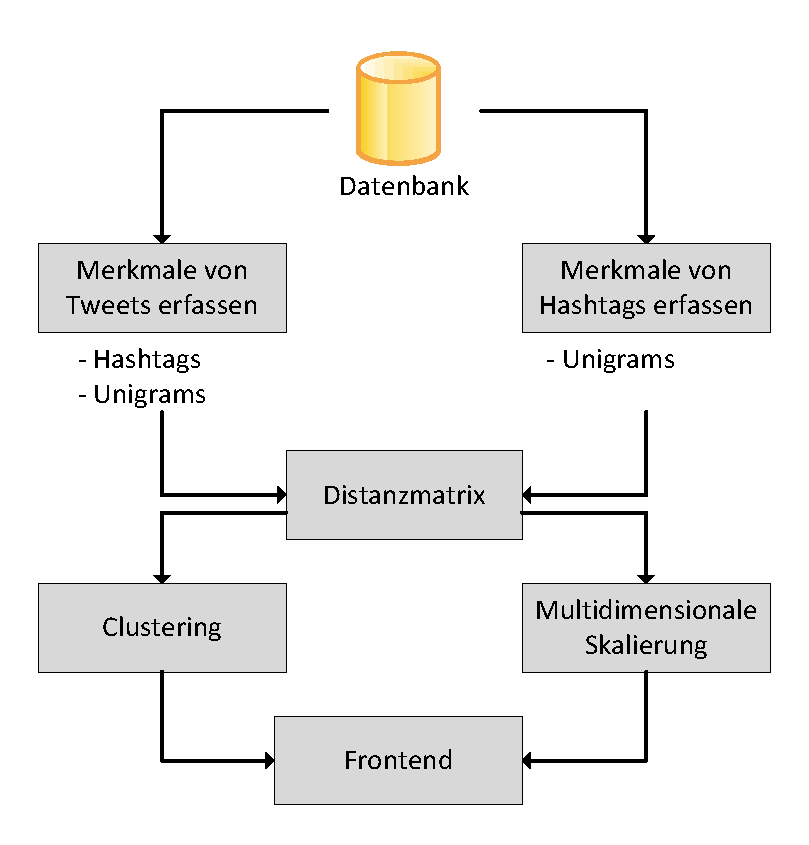
\includegraphics[scale=0.7]{./Bilder/Clustering/ClusteringAufbau.pdf}
\caption{Vorgehensweise bei der Cluster-Analyse}
\label{fig:ClusterVorgehen}
\end{figure}

Bei der Analyse von Tweets stellt die beschränkte Textlänge ein Problem dar, 
wodurch sich nur wenige Informationen extrahieren lassen. Daher wurden schrittweise 
verschiedene Ansätze zur Merkmalsextraktion implementiert, zum Beispiel die Erfassung der 
Hashtags oder der Wörter eines Tweets, auch Unigrams genannt. Diese Ansätze sind in Abschnitt \ref{subsec:ClusterTweets} beschrieben.
Zusätzlich erfolgt eine Cluster-Analyse der Hashtags, welches Kapitel \ref{subsec:ClusterHashtags} beschreibt. 
Hier lassen sich bei der Merkmalsextraktion eines Hashtags alle Tweets, die diesen Hashtag enthalten, heranziehen. 
Damit sind mehr Informationen vorhanden, um einzelne Hashtags zu gruppieren.
Kapitel \ref{subsec:ClusterTweetsWithHashtags} beschreibt einen zweistufigen Ansatz, 
welcher auf Basis der Hashtag"=Cluster versucht, Tweets zu gruppieren. 
Anschließend wird die Distanz der Objekte basierend auf den erhobenen Merkmalen berechnet. 
Mit dem Distanzmaß ist es nun möglich, die eigentliche Cluster"=Analyse 
durch\-zu\-füh\-ren (Kapitel \ref{subsec:ClusterAlgorithmen}). 
Gleichzeitig erfolgt eine Darstellung der Objekte im zweidimensionalen Raum, 
basierend auf den Distanzen (Kapitel \ref{subsec:MDS}). 
Die Cluster"=Zuordnungen sowie die Positionen im zweidimensionalen Raum werden 
anschließend dem Frontend zur grafischen Aufbereitung übergeben.
Das Kapitel schließt mit einer Diskussion der Ergebnisse und gibt einen Ausblick, 
welche Schritte in wei\-te\-ren Scrum"=Iterationen möglich gewesen wären.

%Erwin:
\subsection{Cluster-Analyse von Tweets} \label{subsec:ClusterTweets}

Aus Tweets lassen sich verschiedene Typen von Merkmalen ableiten, mit denen es möglich ist, 
Tweets nach ihrer gegenseitigen Ähnlichkeit zu bewerten. Diese Merkmalstypen werden im Folgenden anhand eines durchgehenden Beispiels erläutert:
\begin{itemize}
\item \textbf{Tweet 1:} \#CDU \#SPD Merkel ist in London
\item \textbf{Tweet 2:} \#CDU \#SPD Merkel reist nach London
\item \textbf{Tweet 3:} Merkel mag \#Rom.
\end{itemize}

%Erwin
\subsubsection{Hashtags als Merkmale}\label{subsec:HashtagsAlsMerkmale}
Die Erfassung der Hashtags eines Tweets stellt die erste Möglichkeit dar, Tweets gegenseitig zu bewerten. 
Da ein Tweet in der Regel keine Wiederholung von Hashtags enthält, 
zählt nur das Auftreten des Hashtags, nicht die Anzahl. 
Damit ist das Hashtag-Merkmal binärkodiert, wobei eine 1 für das Auftreten im Tweet steht. 
Im obigen Beispiel ergibt sich somit die Tabelle \ref{fig:ClusterTab1}. 
Die Zeilen stellen die Tweets dar, die Spalten die erhobenen Merkmale für die Cluster-Analyse.

\begin{table}[ht]
\centering
\begin{tabular}{cccc}
\toprule
 & \#CDU & \#SPD &  \#Rom \\ 
\midrule
Tweet~1 & 1 & 1  & 0 \\ 
 
Tweet~2 & 1 & 1  & 0 \\ 
 
Tweet~3 & 0 & 0  & 1 \\ 
\bottomrule 
\end{tabular} 
\caption{Binäre Merkmale eines Tweets: Hashtags}
\label{fig:ClusterTab1}
\end{table}

Dieses Beispiel erläutert auch die Idee hinter der Hashtag-Erfassung. 
Da Hashtags als Schlagwörter einen Tweet beschreiben, sollten zwei Tweets 
thematisch ähnlicher sein, je mehr übereinstimmende Hashtags sie besitzen.
Im vorliegenden Beispiel sind sich Tweet~1 und Tweet~2 ähnlicher, 
denn beide verwenden die Hashtags \glqq \#CDU\grqq{} und \glqq \#SPD\grqq{}. 

Die Ähnlichkeitserfassung hängt von der Datenskalierung ab. 
Da die Merkmale bi\-när\-ko\-diert sind, kommen Kennzahlen in Frage, 
die die Übereinstimmungen abzählen. Dabei kommen jedoch nur 
Ähnlichkeitsmaße in Frage, bei denen das gleiche Auftreten 
(eine 1er-Übereinstimmung bei jeweils zwei Tweets) eine Rolle spielt. 
Dementsprechend wurden die Ähnlichkeitsmaße Dice, S-Koeffizient, M-Koeffizient und Russel Rao in Betracht gezogen.

%Wladimir
Sei $n_{11}$ die Anzahl der gemeinsam aufgetretenen
Merkmale in zwei Tweets,  $n_{10}$ die Anzahl der Merkmale, die nur im ersten Tweet vorkommen,
$n_{01}$ die Anzahl der Merkmale, die nur im zweiten Tweet vorkommen und 
$n_{00}$ die Anzahl der Merkmale, die in den beiden Tweets nicht vorkommen, dann sind die genannten Ähnlichkeiten
zwi\-schen zwei Tweets wie folgt definiert:
\begin{align*}
& \frac{2n_{11}}{n_{01}+n_{10}+2n_{11}}, \tag{Dice} \\\\
& \frac{n_{11}}{n_{01}+n_{10}+n_{11}}, \tag{S-Koeffizient} \\\\
& \frac{n_{00}+n_{11}}{n_{00}+n_{01}+n_{10}+n_{11}}, \tag{M-Koeffizient}\\\\
& \frac{n_{11}}{n_{00}+n_{01}+n_{10}+n_{11}} \tag{Russel Rao}.
\end{align*}

%\subsection{Wahl der binären Ähnlichkeitsmaße}
%Für die Cluster-Analyse der Tweets mit Hilfe der Hashtags beziehungsweise der Wörter wurden binäre 
%Ahnlichkeitmaße verwendet, siehe Kapitel \ref{subsec:HashtagsAlsMerkmale} und \ref{subsec:WoerterAlsMerkmale}.
%Um einen besseren Eindruck von den unterschiedlichen Ähnlichkeitsmaßen zu bekommen, haben wir ihre Wirkung auf das Ergebnis
%getestet. Die Ähnlichkeitsmaße Dice, S-Koeffizient, M-Koeffizient und Russel Rao wurden in Betracht gezogen, 
%weil sie das gemeinsame Auftreten der Merkmale berücksichtigen. Sei $n_{11}$ die Anzahl der gemeinsam aufgetretenen
%Merkmale in zwei Tweets,  $n_{10}$ die Anzahl der Merkmale, die nur im ersten Tweet vorkamen,
%$n_{01}$ die Anzahl der Merkmale, die nur im zweiten Tweet vorkamen und 
%$n_{00}$ die Anzahl der Merkmale, die in den beiden Tweets nicht vorkamen, dann sind die genannten Ähnlichkeiten
%zwi\-schen zwei Tweets wie folgt definiert:
%\begin{align}
%\frac{2n_{11}}{n_{01}+n_{10}+2n_{11}}, \tag{Dice} \\
%\frac{n_{11}}{n_{01}+n_{10}+n_{11}}, \tag{S-Koeffizient} \\
%\frac{n_{00}+n_{11}}{p}, \tag{M-Koeffizient}\\
%\frac{n_{11}}{p} \tag{Russel Rao}.
%\end{align}

% \def\myDissScale{0.33}
% \begin{figure}[ht]
%    \centering
%       \subcaptionbox{Dice\label{img:Dice}}{\def\maxW{4.23}
\begin{tikzpicture}[scale=\textwidth*\myDissScale/1.0cm, background rectangle/.style={draw=black, thick, fill=yellow!10,},show background rectangle]
\def\marRad{0.20}
\definecolor{color0}{rgb}{0.78,0.89,0.11}
\definecolor{color1}{rgb}{0.10,1.00,0.52}
\definecolor{color2}{rgb}{0.09,0.32,0.64}
\definecolor{color3}{rgb}{0.70,0.69,0.42}
\definecolor{color4}{rgb}{0.36,0.70,0.25}
\definecolor{color5}{rgb}{0.91,0.34,0.56}
\definecolor{color6}{rgb}{0.76,0.33,0.65}
\definecolor{color7}{rgb}{0.06,0.22,0.62}
\definecolor{color8}{rgb}{0.45,0.68,0.87}
\definecolor{color9}{rgb}{0.03,0.89,0.67}
\path[fill=color0,draw=color0,mark size=\marRad, mark=*] plot coordinates {(0.09, -0.43)};
\path[fill=color0,draw=color0,mark size=\marRad, mark=*] plot coordinates {(-0.20, -0.09)};
\path[fill=color0,draw=color0,mark size=\marRad, mark=*] plot coordinates {(-0.03, -0.44)};
\path[fill=color0,draw=color0,mark size=\marRad, mark=*] plot coordinates {(0.41, -0.10)};
\path[fill=color0,draw=color0,mark size=\marRad, mark=*] plot coordinates {(0.11, -0.28)};
\path[fill=color0,draw=color0,mark size=\marRad, mark=*] plot coordinates {(-0.33, -0.14)};
\path[fill=color0,draw=color0,mark size=\marRad, mark=*] plot coordinates {(-0.08, -0.26)};
\path[fill=color0,draw=color0,mark size=\marRad, mark=*] plot coordinates {(0.41, -0.19)};
\path[fill=color0,draw=color0,mark size=\marRad, mark=*] plot coordinates {(0.22, -0.21)};
\path[fill=color0,draw=color0,mark size=\marRad, mark=*] plot coordinates {(-0.28, -0.28)};
\path[fill=color0,draw=color0,mark size=\marRad, mark=*] plot coordinates {(0.41, 0.11)};
\path[fill=color0,draw=color0,mark size=\marRad, mark=*] plot coordinates {(0.43, -0.19)};
\path[fill=color0,draw=color0,mark size=\marRad, mark=*] plot coordinates {(-0.24, -0.03)};
\path[fill=color0,draw=color0,mark size=\marRad, mark=*] plot coordinates {(-0.42, -0.16)};
\path[fill=color0,draw=color0,mark size=\marRad, mark=*] plot coordinates {(-0.25, -0.15)};
\path[fill=color0,draw=color0,mark size=\marRad, mark=*] plot coordinates {(-0.24, -0.15)};
\path[fill=color0,draw=color0,mark size=\marRad, mark=*] plot coordinates {(0.02, -0.41)};
\path[fill=color0,draw=color0,mark size=\marRad, mark=*] plot coordinates {(0.23, -0.01)};
\path[fill=color0,draw=color0,mark size=\marRad, mark=*] plot coordinates {(-0.14, -0.09)};
\path[fill=color0,draw=color0,mark size=\marRad, mark=*] plot coordinates {(0.01, -0.26)};
\path[fill=color0,draw=color0,mark size=\marRad, mark=*] plot coordinates {(0.33, 0.29)};
\path[fill=color0,draw=color0,mark size=\marRad, mark=*] plot coordinates {(0.16, -0.27)};
\path[fill=color0,draw=color0,mark size=\marRad, mark=*] plot coordinates {(0.37, 0.20)};
\path[fill=color0,draw=color0,mark size=\marRad, mark=*] plot coordinates {(-0.41, -0.17)};
\path[fill=color0,draw=color0,mark size=\marRad, mark=*] plot coordinates {(0.33, 0.16)};
\path[fill=color0,draw=color0,mark size=\marRad, mark=*] plot coordinates {(0.25, -0.30)};
\path[fill=color0,draw=color0,mark size=\marRad, mark=*] plot coordinates {(-0.10, -0.22)};
\path[fill=color0,draw=color0,mark size=\marRad, mark=*] plot coordinates {(-0.24, 0.03)};
\path[fill=color0,draw=color0,mark size=\marRad, mark=*] plot coordinates {(0.13, 0.21)};
\path[fill=color0,draw=color0,mark size=\marRad, mark=*] plot coordinates {(0.07, -0.42)};
\path[fill=color0,draw=color0,mark size=\marRad, mark=*] plot coordinates {(0.47, -0.09)};
\path[fill=color0,draw=color0,mark size=\marRad, mark=*] plot coordinates {(0.34, -0.32)};
\path[fill=color0,draw=color0,mark size=\marRad, mark=*] plot coordinates {(0.44, 0.02)};
\path[fill=color0,draw=color0,mark size=\marRad, mark=*] plot coordinates {(0.37, -0.29)};
\path[fill=color0,draw=color0,mark size=\marRad, mark=*] plot coordinates {(-0.08, 0.07)};
\path[fill=color0,draw=color0,mark size=\marRad, mark=*] plot coordinates {(0.09, -0.14)};
\path[fill=color0,draw=color0,mark size=\marRad, mark=*] plot coordinates {(-0.22, -0.13)};
\path[fill=color0,draw=color0,mark size=\marRad, mark=*] plot coordinates {(-0.22, -0.22)};
\path[fill=color0,draw=color0,mark size=\marRad, mark=*] plot coordinates {(0.44, 0.11)};
\path[fill=color0,draw=color0,mark size=\marRad, mark=*] plot coordinates {(0.02, 0.13)};
\path[fill=color0,draw=color0,mark size=\marRad, mark=*] plot coordinates {(-0.17, -0.28)};
\path[fill=color0,draw=color0,mark size=\marRad, mark=*] plot coordinates {(-0.31, 0.01)};
\path[fill=color0,draw=color0,mark size=\marRad, mark=*] plot coordinates {(0.07, -0.22)};
\path[fill=color0,draw=color0,mark size=\marRad, mark=*] plot coordinates {(0.15, -0.42)};
\path[fill=color0,draw=color0,mark size=\marRad, mark=*] plot coordinates {(-0.24, -0.17)};
\path[fill=color0,draw=color0,mark size=\marRad, mark=*] plot coordinates {(0.12, -0.03)};
\path[fill=color0,draw=color0,mark size=\marRad, mark=*] plot coordinates {(-0.19, -0.04)};
\path[fill=color0,draw=color0,mark size=\marRad, mark=*] plot coordinates {(0.10, 0.15)};
\path[fill=color0,draw=color0,mark size=\marRad, mark=*] plot coordinates {(0.39, -0.09)};
\path[fill=color0,draw=color0,mark size=\marRad, mark=*] plot coordinates {(0.33, 0.17)};
\path[fill=color0,draw=color0,mark size=\marRad, mark=*] plot coordinates {(-0.09, -0.23)};
\path[fill=color0,draw=color0,mark size=\marRad, mark=*] plot coordinates {(0.44, 0.04)};
\path[fill=color0,draw=color0,mark size=\marRad, mark=*] plot coordinates {(0.04, 0.03)};
\path[fill=color0,draw=color0,mark size=\marRad, mark=*] plot coordinates {(0.28, -0.31)};
\path[fill=color0,draw=color0,mark size=\marRad, mark=*] plot coordinates {(-0.11, 0.00)};
\path[fill=color0,draw=color0,mark size=\marRad, mark=*] plot coordinates {(0.39, -0.00)};
\path[fill=color0,draw=color0,mark size=\marRad, mark=*] plot coordinates {(0.05, -0.43)};
\path[fill=color0,draw=color0,mark size=\marRad, mark=*] plot coordinates {(-0.03, -0.01)};
\path[fill=color0,draw=color0,mark size=\marRad, mark=*] plot coordinates {(0.24, -0.36)};
\path[fill=color0,draw=color0,mark size=\marRad, mark=*] plot coordinates {(0.07, -0.14)};
\path[fill=color0,draw=color0,mark size=\marRad, mark=*] plot coordinates {(-0.17, -0.20)};
\path[fill=color0,draw=color0,mark size=\marRad, mark=*] plot coordinates {(0.43, -0.21)};
\path[fill=color0,draw=color0,mark size=\marRad, mark=*] plot coordinates {(0.09, -0.19)};
\path[fill=color0,draw=color0,mark size=\marRad, mark=*] plot coordinates {(0.25, -0.34)};
\path[fill=color0,draw=color0,mark size=\marRad, mark=*] plot coordinates {(0.46, 0.12)};
\path[fill=color0,draw=color0,mark size=\marRad, mark=*] plot coordinates {(0.22, -0.18)};
\path[fill=color0,draw=color0,mark size=\marRad, mark=*] plot coordinates {(0.10, 0.02)};
\path[fill=color0,draw=color0,mark size=\marRad, mark=*] plot coordinates {(-0.39, -0.11)};
\path[fill=color0,draw=color0,mark size=\marRad, mark=*] plot coordinates {(0.37, -0.15)};
\path[fill=color0,draw=color0,mark size=\marRad, mark=*] plot coordinates {(0.19, -0.30)};
\path[fill=color0,draw=color0,mark size=\marRad, mark=*] plot coordinates {(-0.01, -0.10)};
\path[fill=color0,draw=color0,mark size=\marRad, mark=*] plot coordinates {(0.16, -0.30)};
\path[fill=color0,draw=color0,mark size=\marRad, mark=*] plot coordinates {(0.34, -0.25)};
\path[fill=color0,draw=color0,mark size=\marRad, mark=*] plot coordinates {(0.32, 0.30)};
\path[fill=color0,draw=color0,mark size=\marRad, mark=*] plot coordinates {(0.31, 0.25)};
\path[fill=color0,draw=color0,mark size=\marRad, mark=*] plot coordinates {(-0.34, -0.15)};
\path[fill=color0,draw=color0,mark size=\marRad, mark=*] plot coordinates {(0.35, 0.02)};
\path[fill=color0,draw=color0,mark size=\marRad, mark=*] plot coordinates {(-0.37, 0.05)};
\path[fill=color0,draw=color0,mark size=\marRad, mark=*] plot coordinates {(0.25, -0.23)};
\path[fill=color0,draw=color0,mark size=\marRad, mark=*] plot coordinates {(0.16, 0.04)};
\path[fill=color0,draw=color0,mark size=\marRad, mark=*] plot coordinates {(0.39, 0.29)};
\path[fill=color0,draw=color0,mark size=\marRad, mark=*] plot coordinates {(0.05, 0.13)};
\path[fill=color0,draw=color0,mark size=\marRad, mark=*] plot coordinates {(-0.32, -0.20)};
\path[fill=color0,draw=color0,mark size=\marRad, mark=*] plot coordinates {(0.32, 0.11)};
\path[fill=color0,draw=color0,mark size=\marRad, mark=*] plot coordinates {(0.38, -0.06)};
\path[fill=color0,draw=color0,mark size=\marRad, mark=*] plot coordinates {(0.42, 0.01)};
\path[fill=color0,draw=color0,mark size=\marRad, mark=*] plot coordinates {(0.32, -0.12)};
\path[fill=color0,draw=color0,mark size=\marRad, mark=*] plot coordinates {(0.29, -0.17)};
\path[fill=color0,draw=color0,mark size=\marRad, mark=*] plot coordinates {(0.17, -0.25)};
\path[fill=color0,draw=color0,mark size=\marRad, mark=*] plot coordinates {(0.33, 0.20)};
\path[fill=color0,draw=color0,mark size=\marRad, mark=*] plot coordinates {(-0.06, -0.03)};
\path[fill=color0,draw=color0,mark size=\marRad, mark=*] plot coordinates {(-0.01, -0.04)};
\path[fill=color0,draw=color0,mark size=\marRad, mark=*] plot coordinates {(0.43, 0.08)};
\path[fill=color0,draw=color0,mark size=\marRad, mark=*] plot coordinates {(-0.34, -0.18)};
\path[fill=color0,draw=color0,mark size=\marRad, mark=*] plot coordinates {(0.39, 0.00)};
\path[fill=color0,draw=color0,mark size=\marRad, mark=*] plot coordinates {(0.17, -0.15)};
\path[fill=color0,draw=color0,mark size=\marRad, mark=*] plot coordinates {(-0.09, -0.11)};
\path[fill=color0,draw=color0,mark size=\marRad, mark=*] plot coordinates {(0.46, 0.07)};
\path[fill=color0,draw=color0,mark size=\marRad, mark=*] plot coordinates {(-0.17, 0.01)};
\path[fill=color0,draw=color0,mark size=\marRad, mark=*] plot coordinates {(0.25, -0.16)};
\path[fill=color0,draw=color0,mark size=\marRad, mark=*] plot coordinates {(0.01, -0.21)};
\path[fill=color0,draw=color0,mark size=\marRad, mark=*] plot coordinates {(0.33, -0.01)};
\path[fill=color0,draw=color0,mark size=\marRad, mark=*] plot coordinates {(0.07, -0.34)};
\path[fill=color0,draw=color0,mark size=\marRad, mark=*] plot coordinates {(-0.20, -0.00)};
\path[fill=color0,draw=color0,mark size=\marRad, mark=*] plot coordinates {(0.02, -0.35)};
\path[fill=color0,draw=color0,mark size=\marRad, mark=*] plot coordinates {(0.39, -0.13)};
\path[fill=color0,draw=color0,mark size=\marRad, mark=*] plot coordinates {(-0.20, -0.24)};
\path[fill=color0,draw=color0,mark size=\marRad, mark=*] plot coordinates {(0.11, -0.44)};
\path[fill=color0,draw=color0,mark size=\marRad, mark=*] plot coordinates {(0.46, -0.01)};
\path[fill=color0,draw=color0,mark size=\marRad, mark=*] plot coordinates {(0.26, -0.39)};
\path[fill=color0,draw=color0,mark size=\marRad, mark=*] plot coordinates {(-0.17, -0.35)};
\path[fill=color0,draw=color0,mark size=\marRad, mark=*] plot coordinates {(-0.26, 0.05)};
\path[fill=color0,draw=color0,mark size=\marRad, mark=*] plot coordinates {(-0.08, -0.41)};
\path[fill=color0,draw=color0,mark size=\marRad, mark=*] plot coordinates {(0.28, -0.25)};
\path[fill=color0,draw=color0,mark size=\marRad, mark=*] plot coordinates {(-0.19, -0.17)};
\path[fill=color0,draw=color0,mark size=\marRad, mark=*] plot coordinates {(0.28, -0.11)};
\path[fill=color0,draw=color0,mark size=\marRad, mark=*] plot coordinates {(-0.01, -0.01)};
\path[fill=color0,draw=color0,mark size=\marRad, mark=*] plot coordinates {(-0.01, 0.08)};
\path[fill=color0,draw=color0,mark size=\marRad, mark=*] plot coordinates {(0.20, 0.13)};
\path[fill=color0,draw=color0,mark size=\marRad, mark=*] plot coordinates {(0.49, 0.02)};
\path[fill=color0,draw=color0,mark size=\marRad, mark=*] plot coordinates {(0.22, -0.42)};
\path[fill=color0,draw=color0,mark size=\marRad, mark=*] plot coordinates {(0.35, -0.19)};
\path[fill=color0,draw=color0,mark size=\marRad, mark=*] plot coordinates {(-0.07, 0.04)};
\path[fill=color0,draw=color0,mark size=\marRad, mark=*] plot coordinates {(0.30, -0.29)};
\path[fill=color0,draw=color0,mark size=\marRad, mark=*] plot coordinates {(0.11, 0.11)};
\path[fill=color0,draw=color0,mark size=\marRad, mark=*] plot coordinates {(0.29, 0.16)};
\path[fill=color0,draw=color0,mark size=\marRad, mark=*] plot coordinates {(0.44, 0.21)};
\path[fill=color0,draw=color0,mark size=\marRad, mark=*] plot coordinates {(-0.35, -0.10)};
\path[fill=color0,draw=color0,mark size=\marRad, mark=*] plot coordinates {(0.29, -0.38)};
\path[fill=color0,draw=color0,mark size=\marRad, mark=*] plot coordinates {(0.28, 0.10)};
\path[fill=color0,draw=color0,mark size=\marRad, mark=*] plot coordinates {(0.33, -0.14)};
\path[fill=color0,draw=color0,mark size=\marRad, mark=*] plot coordinates {(0.40, -0.28)};
\path[fill=color0,draw=color0,mark size=\marRad, mark=*] plot coordinates {(0.23, 0.11)};
\path[fill=color0,draw=color0,mark size=\marRad, mark=*] plot coordinates {(-0.18, -0.29)};
\path[fill=color0,draw=color0,mark size=\marRad, mark=*] plot coordinates {(0.17, -0.01)};
\path[fill=color0,draw=color0,mark size=\marRad, mark=*] plot coordinates {(0.10, -0.47)};
\path[fill=color0,draw=color0,mark size=\marRad, mark=*] plot coordinates {(0.33, -0.06)};
\path[fill=color0,draw=color0,mark size=\marRad, mark=*] plot coordinates {(0.09, -0.26)};
\path[fill=color0,draw=color0,mark size=\marRad, mark=*] plot coordinates {(0.36, 0.04)};
\path[fill=color0,draw=color0,mark size=\marRad, mark=*] plot coordinates {(0.33, -0.02)};
\path[fill=color0,draw=color0,mark size=\marRad, mark=*] plot coordinates {(0.15, -0.36)};
\path[fill=color0,draw=color0,mark size=\marRad, mark=*] plot coordinates {(0.45, -0.06)};
\path[fill=color0,draw=color0,mark size=\marRad, mark=*] plot coordinates {(-0.27, -0.11)};
\path[fill=color0,draw=color0,mark size=\marRad, mark=*] plot coordinates {(0.43, 0.08)};
\path[fill=color0,draw=color0,mark size=\marRad, mark=*] plot coordinates {(-0.38, -0.25)};
\path[fill=color0,draw=color0,mark size=\marRad, mark=*] plot coordinates {(0.27, -0.40)};
\path[fill=color0,draw=color0,mark size=\marRad, mark=*] plot coordinates {(0.16, -0.40)};
\path[fill=color0,draw=color0,mark size=\marRad, mark=*] plot coordinates {(-0.30, -0.27)};
\path[fill=color0,draw=color0,mark size=\marRad, mark=*] plot coordinates {(0.10, -0.45)};
\path[fill=color0,draw=color0,mark size=\marRad, mark=*] plot coordinates {(0.37, 0.05)};
\path[fill=color0,draw=color0,mark size=\marRad, mark=*] plot coordinates {(0.15, -0.40)};
\path[fill=color0,draw=color0,mark size=\marRad, mark=*] plot coordinates {(-0.04, -0.14)};
\path[fill=color0,draw=color0,mark size=\marRad, mark=*] plot coordinates {(0.46, 0.06)};
\path[fill=color0,draw=color0,mark size=\marRad, mark=*] plot coordinates {(0.37, 0.30)};
\path[fill=color0,draw=color0,mark size=\marRad, mark=*] plot coordinates {(0.34, 0.09)};
\path[fill=color0,draw=color0,mark size=\marRad, mark=*] plot coordinates {(-0.04, 0.09)};
\path[fill=color0,draw=color0,mark size=\marRad, mark=*] plot coordinates {(0.41, -0.06)};
\path[fill=color0,draw=color0,mark size=\marRad, mark=*] plot coordinates {(0.35, -0.25)};
\path[fill=color0,draw=color0,mark size=\marRad, mark=*] plot coordinates {(-0.13, -0.17)};
\path[fill=color0,draw=color0,mark size=\marRad, mark=*] plot coordinates {(0.41, -0.12)};
\path[fill=color0,draw=color0,mark size=\marRad, mark=*] plot coordinates {(0.18, -0.41)};
\path[fill=color0,draw=color0,mark size=\marRad, mark=*] plot coordinates {(-0.09, -0.03)};
\path[fill=color0,draw=color0,mark size=\marRad, mark=*] plot coordinates {(0.01, -0.46)};
\path[fill=color0,draw=color0,mark size=\marRad, mark=*] plot coordinates {(0.35, -0.16)};
\path[fill=color0,draw=color0,mark size=\marRad, mark=*] plot coordinates {(0.24, 0.13)};
\path[fill=color0,draw=color0,mark size=\marRad, mark=*] plot coordinates {(0.25, 0.20)};
\path[fill=color0,draw=color0,mark size=\marRad, mark=*] plot coordinates {(0.42, 0.14)};
\path[fill=color0,draw=color0,mark size=\marRad, mark=*] plot coordinates {(0.36, -0.04)};
\path[fill=color0,draw=color0,mark size=\marRad, mark=*] plot coordinates {(0.11, -0.13)};
\path[fill=color0,draw=color0,mark size=\marRad, mark=*] plot coordinates {(0.09, -0.07)};
\path[fill=color0,draw=color0,mark size=\marRad, mark=*] plot coordinates {(-0.19, -0.37)};
\path[fill=color0,draw=color0,mark size=\marRad, mark=*] plot coordinates {(0.17, 0.03)};
\path[fill=color0,draw=color0,mark size=\marRad, mark=*] plot coordinates {(0.20, -0.35)};
\path[fill=color0,draw=color0,mark size=\marRad, mark=*] plot coordinates {(0.29, 0.09)};
\path[fill=color0,draw=color0,mark size=\marRad, mark=*] plot coordinates {(0.45, -0.18)};
\path[fill=color0,draw=color0,mark size=\marRad, mark=*] plot coordinates {(0.44, 0.04)};
\path[fill=color0,draw=color0,mark size=\marRad, mark=*] plot coordinates {(0.35, -0.12)};
\path[fill=color0,draw=color0,mark size=\marRad, mark=*] plot coordinates {(0.39, 0.26)};
\path[fill=color0,draw=color0,mark size=\marRad, mark=*] plot coordinates {(-0.23, -0.33)};
\path[fill=color0,draw=color0,mark size=\marRad, mark=*] plot coordinates {(-0.04, -0.16)};
\path[fill=color0,draw=color0,mark size=\marRad, mark=*] plot coordinates {(0.33, -0.31)};
\path[fill=color0,draw=color0,mark size=\marRad, mark=*] plot coordinates {(0.42, -0.05)};
\path[fill=color0,draw=color0,mark size=\marRad, mark=*] plot coordinates {(-0.01, -0.15)};
\path[fill=color0,draw=color0,mark size=\marRad, mark=*] plot coordinates {(0.46, -0.10)};
\path[fill=color0,draw=color0,mark size=\marRad, mark=*] plot coordinates {(0.24, -0.22)};
\path[fill=color0,draw=color0,mark size=\marRad, mark=*] plot coordinates {(0.12, -0.22)};
\path[fill=color0,draw=color0,mark size=\marRad, mark=*] plot coordinates {(-0.16, -0.43)};
\path[fill=color0,draw=color0,mark size=\marRad, mark=*] plot coordinates {(0.35, -0.34)};
\path[fill=color0,draw=color0,mark size=\marRad, mark=*] plot coordinates {(0.45, -0.18)};
\path[fill=color0,draw=color0,mark size=\marRad, mark=*] plot coordinates {(-0.13, -0.19)};
\path[fill=color0,draw=color0,mark size=\marRad, mark=*] plot coordinates {(0.02, 0.10)};
\path[fill=color0,draw=color0,mark size=\marRad, mark=*] plot coordinates {(0.13, 0.05)};
\path[fill=color0,draw=color0,mark size=\marRad, mark=*] plot coordinates {(0.12, -0.38)};
\path[fill=color0,draw=color0,mark size=\marRad, mark=*] plot coordinates {(0.19, -0.42)};
\path[fill=color0,draw=color0,mark size=\marRad, mark=*] plot coordinates {(0.19, -0.13)};
\path[fill=color0,draw=color0,mark size=\marRad, mark=*] plot coordinates {(0.19, -0.42)};
\path[fill=color0,draw=color0,mark size=\marRad, mark=*] plot coordinates {(-0.36, 0.03)};
\path[fill=color0,draw=color0,mark size=\marRad, mark=*] plot coordinates {(-0.30, -0.03)};
\path[fill=color0,draw=color0,mark size=\marRad, mark=*] plot coordinates {(0.47, -0.09)};
\path[fill=color0,draw=color0,mark size=\marRad, mark=*] plot coordinates {(0.31, -0.37)};
\path[fill=color0,draw=color0,mark size=\marRad, mark=*] plot coordinates {(0.38, 0.06)};
\path[fill=color0,draw=color0,mark size=\marRad, mark=*] plot coordinates {(-0.33, -0.19)};
\path[fill=color0,draw=color0,mark size=\marRad, mark=*] plot coordinates {(-0.08, -0.45)};
\path[fill=color0,draw=color0,mark size=\marRad, mark=*] plot coordinates {(0.16, -0.30)};
\path[fill=color0,draw=color0,mark size=\marRad, mark=*] plot coordinates {(-0.03, -0.24)};
\path[fill=color0,draw=color0,mark size=\marRad, mark=*] plot coordinates {(-0.06, -0.36)};
\path[fill=color0,draw=color0,mark size=\marRad, mark=*] plot coordinates {(0.44, 0.19)};
\path[fill=color0,draw=color0,mark size=\marRad, mark=*] plot coordinates {(0.06, -0.20)};
\path[fill=color0,draw=color0,mark size=\marRad, mark=*] plot coordinates {(-0.33, -0.03)};
\path[fill=color0,draw=color0,mark size=\marRad, mark=*] plot coordinates {(-0.24, -0.37)};
\path[fill=color0,draw=color0,mark size=\marRad, mark=*] plot coordinates {(0.01, -0.08)};
\path[fill=color0,draw=color0,mark size=\marRad, mark=*] plot coordinates {(0.21, -0.24)};
\path[fill=color0,draw=color0,mark size=\marRad, mark=*] plot coordinates {(0.24, -0.40)};
\path[fill=color0,draw=color0,mark size=\marRad, mark=*] plot coordinates {(0.36, 0.26)};
\path[fill=color0,draw=color0,mark size=\marRad, mark=*] plot coordinates {(-0.14, 0.04)};
\path[fill=color0,draw=color0,mark size=\marRad, mark=*] plot coordinates {(-0.01, -0.43)};
\path[fill=color0,draw=color0,mark size=\marRad, mark=*] plot coordinates {(-0.25, -0.24)};
\path[fill=color0,draw=color0,mark size=\marRad, mark=*] plot coordinates {(0.26, -0.29)};
\path[fill=color0,draw=color0,mark size=\marRad, mark=*] plot coordinates {(0.01, -0.31)};
\path[fill=color0,draw=color0,mark size=\marRad, mark=*] plot coordinates {(0.36, 0.21)};
\path[fill=color0,draw=color0,mark size=\marRad, mark=*] plot coordinates {(0.22, -0.20)};
\path[fill=color0,draw=color0,mark size=\marRad, mark=*] plot coordinates {(-0.03, -0.21)};
\path[fill=color0,draw=color0,mark size=\marRad, mark=*] plot coordinates {(-0.18, -0.28)};
\path[fill=color0,draw=color0,mark size=\marRad, mark=*] plot coordinates {(0.48, 0.09)};
\path[fill=color0,draw=color0,mark size=\marRad, mark=*] plot coordinates {(-0.22, -0.11)};
\path[fill=color0,draw=color0,mark size=\marRad, mark=*] plot coordinates {(0.37, -0.23)};
\path[fill=color0,draw=color0,mark size=\marRad, mark=*] plot coordinates {(-0.41, 0.03)};
\path[fill=color0,draw=color0,mark size=\marRad, mark=*] plot coordinates {(0.01, -0.23)};
\path[fill=color0,draw=color0,mark size=\marRad, mark=*] plot coordinates {(0.20, 0.17)};
\path[fill=color0,draw=color0,mark size=\marRad, mark=*] plot coordinates {(-0.04, -0.22)};
\path[fill=color0,draw=color0,mark size=\marRad, mark=*] plot coordinates {(-0.39, -0.00)};
\path[fill=color0,draw=color0,mark size=\marRad, mark=*] plot coordinates {(-0.26, -0.05)};
\path[fill=color0,draw=color0,mark size=\marRad, mark=*] plot coordinates {(0.45, -0.14)};
\path[fill=color0,draw=color0,mark size=\marRad, mark=*] plot coordinates {(-0.33, -0.27)};
\path[fill=color0,draw=color0,mark size=\marRad, mark=*] plot coordinates {(0.19, 0.11)};
\path[fill=color0,draw=color0,mark size=\marRad, mark=*] plot coordinates {(0.35, -0.30)};
\path[fill=color0,draw=color0,mark size=\marRad, mark=*] plot coordinates {(-0.19, 0.01)};
\path[fill=color0,draw=color0,mark size=\marRad, mark=*] plot coordinates {(0.34, -0.34)};
\path[fill=color0,draw=color0,mark size=\marRad, mark=*] plot coordinates {(0.31, -0.28)};
\path[fill=color0,draw=color0,mark size=\marRad, mark=*] plot coordinates {(0.25, -0.14)};
\path[fill=color0,draw=color0,mark size=\marRad, mark=*] plot coordinates {(0.28, -0.07)};
\path[fill=color0,draw=color0,mark size=\marRad, mark=*] plot coordinates {(0.28, -0.33)};
\path[fill=color0,draw=color0,mark size=\marRad, mark=*] plot coordinates {(0.34, -0.07)};
\path[fill=color0,draw=color0,mark size=\marRad, mark=*] plot coordinates {(0.29, -0.20)};
\path[fill=color0,draw=color0,mark size=\marRad, mark=*] plot coordinates {(-0.15, -0.05)};
\path[fill=color0,draw=color0,mark size=\marRad, mark=*] plot coordinates {(-0.40, -0.04)};
\path[fill=color0,draw=color0,mark size=\marRad, mark=*] plot coordinates {(-0.14, -0.30)};
\path[fill=color0,draw=color0,mark size=\marRad, mark=*] plot coordinates {(0.20, 0.06)};
\path[fill=color0,draw=color0,mark size=\marRad, mark=*] plot coordinates {(0.46, 0.17)};
\path[fill=color0,draw=color0,mark size=\marRad, mark=*] plot coordinates {(-0.05, -0.20)};
\path[fill=color0,draw=color0,mark size=\marRad, mark=*] plot coordinates {(0.13, -0.14)};
\path[fill=color0,draw=color0,mark size=\marRad, mark=*] plot coordinates {(0.28, -0.13)};
\path[fill=color0,draw=color0,mark size=\marRad, mark=*] plot coordinates {(0.15, 0.06)};
\path[fill=color0,draw=color0,mark size=\marRad, mark=*] plot coordinates {(0.22, -0.16)};
\path[fill=color0,draw=color0,mark size=\marRad, mark=*] plot coordinates {(0.02, -0.04)};
\path[fill=color0,draw=color0,mark size=\marRad, mark=*] plot coordinates {(-0.02, -0.05)};
\path[fill=color0,draw=color0,mark size=\marRad, mark=*] plot coordinates {(0.31, 0.11)};
\path[fill=color0,draw=color0,mark size=\marRad, mark=*] plot coordinates {(0.10, 0.01)};
\path[fill=color0,draw=color0,mark size=\marRad, mark=*] plot coordinates {(0.21, -0.09)};
\path[fill=color0,draw=color0,mark size=\marRad, mark=*] plot coordinates {(0.21, -0.10)};
\path[fill=color0,draw=color0,mark size=\marRad, mark=*] plot coordinates {(0.24, -0.02)};
\path[fill=color0,draw=color0,mark size=\marRad, mark=*] plot coordinates {(0.30, 0.13)};
\path[fill=color0,draw=color0,mark size=\marRad, mark=*] plot coordinates {(0.03, -0.14)};
\path[fill=color0,draw=color0,mark size=\marRad, mark=*] plot coordinates {(-0.23, -0.08)};
\path[fill=color0,draw=color0,mark size=\marRad, mark=*] plot coordinates {(-0.03, -0.17)};
\path[fill=color0,draw=color0,mark size=\marRad, mark=*] plot coordinates {(0.11, -0.38)};
\path[fill=color0,draw=color0,mark size=\marRad, mark=*] plot coordinates {(-0.23, -0.28)};
\path[fill=color0,draw=color0,mark size=\marRad, mark=*] plot coordinates {(-0.17, -0.15)};
\path[fill=color0,draw=color0,mark size=\marRad, mark=*] plot coordinates {(0.13, -0.20)};
\path[fill=color0,draw=color0,mark size=\marRad, mark=*] plot coordinates {(-0.44, -0.10)};
\path[fill=color0,draw=color0,mark size=\marRad, mark=*] plot coordinates {(0.38, 0.13)};
\path[fill=color0,draw=color0,mark size=\marRad, mark=*] plot coordinates {(0.12, -0.13)};
\path[fill=color0,draw=color0,mark size=\marRad, mark=*] plot coordinates {(0.43, 0.17)};
\path[fill=color0,draw=color0,mark size=\marRad, mark=*] plot coordinates {(0.37, 0.19)};
\path[fill=color0,draw=color0,mark size=\marRad, mark=*] plot coordinates {(-0.22, -0.00)};
\path[fill=color0,draw=color0,mark size=\marRad, mark=*] plot coordinates {(-0.14, -0.18)};
\path[fill=color0,draw=color0,mark size=\marRad, mark=*] plot coordinates {(-0.38, -0.10)};
\path[fill=color0,draw=color0,mark size=\marRad, mark=*] plot coordinates {(-0.19, -0.04)};
\path[fill=color0,draw=color0,mark size=\marRad, mark=*] plot coordinates {(0.02, -0.16)};
\path[fill=color0,draw=color0,mark size=\marRad, mark=*] plot coordinates {(0.26, 0.12)};
\path[fill=color0,draw=color0,mark size=\marRad, mark=*] plot coordinates {(-0.03, -0.30)};
\path[fill=color0,draw=color0,mark size=\marRad, mark=*] plot coordinates {(0.19, -0.34)};
\path[fill=color0,draw=color0,mark size=\marRad, mark=*] plot coordinates {(0.03, -0.10)};
\path[fill=color0,draw=color0,mark size=\marRad, mark=*] plot coordinates {(0.40, 0.07)};
\path[fill=color0,draw=color0,mark size=\marRad, mark=*] plot coordinates {(-0.12, 0.10)};
\path[fill=color0,draw=color0,mark size=\marRad, mark=*] plot coordinates {(-0.01, -0.15)};
\path[fill=color0,draw=color0,mark size=\marRad, mark=*] plot coordinates {(-0.09, -0.32)};
\path[fill=color0,draw=color0,mark size=\marRad, mark=*] plot coordinates {(0.13, 0.22)};
\path[fill=color0,draw=color0,mark size=\marRad, mark=*] plot coordinates {(0.31, -0.39)};
\path[fill=color0,draw=color0,mark size=\marRad, mark=*] plot coordinates {(0.06, -0.16)};
\path[fill=color0,draw=color0,mark size=\marRad, mark=*] plot coordinates {(-0.40, -0.00)};
\path[fill=color0,draw=color0,mark size=\marRad, mark=*] plot coordinates {(0.39, 0.18)};
\path[fill=color0,draw=color0,mark size=\marRad, mark=*] plot coordinates {(0.16, -0.05)};
\path[fill=color0,draw=color0,mark size=\marRad, mark=*] plot coordinates {(-0.42, -0.07)};
\path[fill=color0,draw=color0,mark size=\marRad, mark=*] plot coordinates {(-0.44, -0.16)};
\path[fill=color0,draw=color0,mark size=\marRad, mark=*] plot coordinates {(0.07, -0.25)};
\path[fill=color0,draw=color0,mark size=\marRad, mark=*] plot coordinates {(0.06, -0.35)};
\path[fill=color0,draw=color0,mark size=\marRad, mark=*] plot coordinates {(-0.21, -0.27)};
\path[fill=color0,draw=color0,mark size=\marRad, mark=*] plot coordinates {(0.39, -0.10)};
\path[fill=color0,draw=color0,mark size=\marRad, mark=*] plot coordinates {(0.09, 0.11)};
\path[fill=color0,draw=color0,mark size=\marRad, mark=*] plot coordinates {(0.18, 0.07)};
\path[fill=color0,draw=color0,mark size=\marRad, mark=*] plot coordinates {(-0.13, -0.34)};
\path[fill=color0,draw=color0,mark size=\marRad, mark=*] plot coordinates {(0.16, -0.02)};
\path[fill=color0,draw=color0,mark size=\marRad, mark=*] plot coordinates {(0.23, 0.24)};
\path[fill=color0,draw=color0,mark size=\marRad, mark=*] plot coordinates {(0.35, -0.08)};
\path[fill=color0,draw=color0,mark size=\marRad, mark=*] plot coordinates {(0.34, -0.14)};
\path[fill=color0,draw=color0,mark size=\marRad, mark=*] plot coordinates {(0.39, 0.28)};
\path[fill=color0,draw=color0,mark size=\marRad, mark=*] plot coordinates {(-0.02, 0.12)};
\path[fill=color0,draw=color0,mark size=\marRad, mark=*] plot coordinates {(0.01, -0.49)};
\path[fill=color0,draw=color0,mark size=\marRad, mark=*] plot coordinates {(0.11, -0.04)};
\path[fill=color0,draw=color0,mark size=\marRad, mark=*] plot coordinates {(-0.42, 0.01)};
\path[fill=color0,draw=color0,mark size=\marRad, mark=*] plot coordinates {(0.15, -0.44)};
\path[fill=color0,draw=color0,mark size=\marRad, mark=*] plot coordinates {(0.04, -0.02)};
\path[fill=color0,draw=color0,mark size=\marRad, mark=*] plot coordinates {(0.33, -0.20)};
\path[fill=color0,draw=color0,mark size=\marRad, mark=*] plot coordinates {(-0.11, -0.29)};
\path[fill=color0,draw=color0,mark size=\marRad, mark=*] plot coordinates {(0.24, 0.13)};
\path[fill=color0,draw=color0,mark size=\marRad, mark=*] plot coordinates {(0.08, -0.34)};
\path[fill=color0,draw=color0,mark size=\marRad, mark=*] plot coordinates {(-0.39, -0.07)};
\path[fill=color0,draw=color0,mark size=\marRad, mark=*] plot coordinates {(0.23, 0.16)};
\path[fill=color0,draw=color0,mark size=\marRad, mark=*] plot coordinates {(0.06, -0.26)};
\path[fill=color0,draw=color0,mark size=\marRad, mark=*] plot coordinates {(-0.10, -0.05)};
\path[fill=color0,draw=color0,mark size=\marRad, mark=*] plot coordinates {(-0.34, -0.08)};
\path[fill=color0,draw=color0,mark size=\marRad, mark=*] plot coordinates {(-0.16, -0.08)};
\path[fill=color0,draw=color0,mark size=\marRad, mark=*] plot coordinates {(0.21, -0.33)};
\path[fill=color0,draw=color0,mark size=\marRad, mark=*] plot coordinates {(0.25, -0.40)};
\path[fill=color0,draw=color0,mark size=\marRad, mark=*] plot coordinates {(0.47, -0.02)};
\path[fill=color0,draw=color0,mark size=\marRad, mark=*] plot coordinates {(0.39, -0.25)};
\path[fill=color0,draw=color0,mark size=\marRad, mark=*] plot coordinates {(0.33, 0.03)};
\path[fill=color0,draw=color0,mark size=\marRad, mark=*] plot coordinates {(0.35, -0.26)};
\path[fill=color0,draw=color0,mark size=\marRad, mark=*] plot coordinates {(0.43, 0.11)};
\path[fill=color0,draw=color0,mark size=\marRad, mark=*] plot coordinates {(-0.42, -0.03)};
\path[fill=color0,draw=color0,mark size=\marRad, mark=*] plot coordinates {(0.07, -0.24)};
\path[fill=color0,draw=color0,mark size=\marRad, mark=*] plot coordinates {(-0.03, -0.23)};
\path[fill=color0,draw=color0,mark size=\marRad, mark=*] plot coordinates {(0.21, 0.04)};
\path[fill=color0,draw=color0,mark size=\marRad, mark=*] plot coordinates {(0.03, -0.04)};
\path[fill=color0,draw=color0,mark size=\marRad, mark=*] plot coordinates {(-0.17, -0.18)};
\path[fill=color0,draw=color0,mark size=\marRad, mark=*] plot coordinates {(0.37, -0.09)};
\path[fill=color0,draw=color0,mark size=\marRad, mark=*] plot coordinates {(0.21, -0.30)};
\path[fill=color0,draw=color0,mark size=\marRad, mark=*] plot coordinates {(0.39, -0.22)};
\path[fill=color0,draw=color0,mark size=\marRad, mark=*] plot coordinates {(-0.38, -0.28)};
\path[fill=color0,draw=color0,mark size=\marRad, mark=*] plot coordinates {(0.23, 0.04)};
\path[fill=color0,draw=color0,mark size=\marRad, mark=*] plot coordinates {(-0.08, -0.06)};
\path[fill=color0,draw=color0,mark size=\marRad, mark=*] plot coordinates {(0.23, 0.12)};
\path[fill=color0,draw=color0,mark size=\marRad, mark=*] plot coordinates {(-0.13, -0.03)};
\path[fill=color0,draw=color0,mark size=\marRad, mark=*] plot coordinates {(0.06, -0.36)};
\path[fill=color0,draw=color0,mark size=\marRad, mark=*] plot coordinates {(-0.21, 0.02)};
\path[fill=color0,draw=color0,mark size=\marRad, mark=*] plot coordinates {(0.43, -0.05)};
\path[fill=color0,draw=color0,mark size=\marRad, mark=*] plot coordinates {(-0.18, 0.10)};
\path[fill=color0,draw=color0,mark size=\marRad, mark=*] plot coordinates {(0.29, 0.26)};
\path[fill=color0,draw=color0,mark size=\marRad, mark=*] plot coordinates {(-0.01, -0.39)};
\path[fill=color0,draw=color0,mark size=\marRad, mark=*] plot coordinates {(0.24, 0.07)};
\path[fill=color0,draw=color0,mark size=\marRad, mark=*] plot coordinates {(0.48, -0.00)};
\path[fill=color0,draw=color0,mark size=\marRad, mark=*] plot coordinates {(0.30, -0.06)};
\path[fill=color0,draw=color0,mark size=\marRad, mark=*] plot coordinates {(0.06, -0.36)};
\path[fill=color0,draw=color0,mark size=\marRad, mark=*] plot coordinates {(0.33, -0.14)};
\path[fill=color0,draw=color0,mark size=\marRad, mark=*] plot coordinates {(0.12, -0.34)};
\path[fill=color0,draw=color0,mark size=\marRad, mark=*] plot coordinates {(0.41, -0.27)};
\path[fill=color0,draw=color0,mark size=\marRad, mark=*] plot coordinates {(-0.31, -0.02)};
\path[fill=color0,draw=color0,mark size=\marRad, mark=*] plot coordinates {(0.18, -0.19)};
\path[fill=color0,draw=color0,mark size=\marRad, mark=*] plot coordinates {(0.15, -0.37)};
\path[fill=color0,draw=color0,mark size=\marRad, mark=*] plot coordinates {(-0.06, -0.35)};
\path[fill=color0,draw=color0,mark size=\marRad, mark=*] plot coordinates {(0.25, -0.29)};
\path[fill=color0,draw=color0,mark size=\marRad, mark=*] plot coordinates {(0.43, 0.19)};
\path[fill=color0,draw=color0,mark size=\marRad, mark=*] plot coordinates {(0.34, -0.29)};
\path[fill=color0,draw=color0,mark size=\marRad, mark=*] plot coordinates {(0.48, -0.05)};
\path[fill=color0,draw=color0,mark size=\marRad, mark=*] plot coordinates {(0.41, 0.25)};
\path[fill=color0,draw=color0,mark size=\marRad, mark=*] plot coordinates {(-0.31, -0.20)};
\path[fill=color0,draw=color0,mark size=\marRad, mark=*] plot coordinates {(0.20, 0.02)};
\path[fill=color0,draw=color0,mark size=\marRad, mark=*] plot coordinates {(-0.11, 0.08)};
\path[fill=color0,draw=color0,mark size=\marRad, mark=*] plot coordinates {(0.08, 0.07)};
\path[fill=color0,draw=color0,mark size=\marRad, mark=*] plot coordinates {(0.09, -0.28)};
\path[fill=color0,draw=color0,mark size=\marRad, mark=*] plot coordinates {(0.08, -0.42)};
\path[fill=color0,draw=color0,mark size=\marRad, mark=*] plot coordinates {(-0.39, -0.18)};
\path[fill=color0,draw=color0,mark size=\marRad, mark=*] plot coordinates {(0.16, 0.15)};
\path[fill=color0,draw=color0,mark size=\marRad, mark=*] plot coordinates {(0.15, -0.11)};
\path[fill=color0,draw=color0,mark size=\marRad, mark=*] plot coordinates {(0.04, -0.48)};
\path[fill=color0,draw=color0,mark size=\marRad, mark=*] plot coordinates {(0.13, -0.20)};
\path[fill=color0,draw=color0,mark size=\marRad, mark=*] plot coordinates {(0.38, 0.03)};
\path[fill=color0,draw=color0,mark size=\marRad, mark=*] plot coordinates {(0.35, 0.23)};
\path[fill=color0,draw=color0,mark size=\marRad, mark=*] plot coordinates {(0.18, -0.36)};
\path[fill=color0,draw=color0,mark size=\marRad, mark=*] plot coordinates {(0.04, -0.43)};
\path[fill=color0,draw=color0,mark size=\marRad, mark=*] plot coordinates {(0.22, -0.40)};
\path[fill=color0,draw=color0,mark size=\marRad, mark=*] plot coordinates {(0.15, -0.18)};
\path[fill=color0,draw=color0,mark size=\marRad, mark=*] plot coordinates {(-0.34, -0.06)};
\path[fill=color0,draw=color0,mark size=\marRad, mark=*] plot coordinates {(-0.03, -0.35)};
\path[fill=color0,draw=color0,mark size=\marRad, mark=*] plot coordinates {(-0.01, 0.01)};
\path[fill=color0,draw=color0,mark size=\marRad, mark=*] plot coordinates {(0.32, 0.18)};
\path[fill=color0,draw=color0,mark size=\marRad, mark=*] plot coordinates {(-0.14, -0.39)};
\path[fill=color0,draw=color0,mark size=\marRad, mark=*] plot coordinates {(0.06, -0.48)};
\path[fill=color0,draw=color0,mark size=\marRad, mark=*] plot coordinates {(0.16, 0.16)};
\path[fill=color0,draw=color0,mark size=\marRad, mark=*] plot coordinates {(-0.25, -0.10)};
\path[fill=color0,draw=color0,mark size=\marRad, mark=*] plot coordinates {(0.48, 0.14)};
\path[fill=color0,draw=color0,mark size=\marRad, mark=*] plot coordinates {(0.28, -0.36)};
\path[fill=color0,draw=color0,mark size=\marRad, mark=*] plot coordinates {(0.30, 0.23)};
\path[fill=color0,draw=color0,mark size=\marRad, mark=*] plot coordinates {(0.28, 0.26)};
\path[fill=color0,draw=color0,mark size=\marRad, mark=*] plot coordinates {(0.34, 0.09)};
\path[fill=color0,draw=color0,mark size=\marRad, mark=*] plot coordinates {(0.40, -0.01)};
\path[fill=color0,draw=color0,mark size=\marRad, mark=*] plot coordinates {(-0.27, -0.02)};
\path[fill=color0,draw=color0,mark size=\marRad, mark=*] plot coordinates {(0.35, 0.16)};
\path[fill=color0,draw=color0,mark size=\marRad, mark=*] plot coordinates {(0.03, 0.05)};
\path[fill=color0,draw=color0,mark size=\marRad, mark=*] plot coordinates {(0.28, 0.16)};
\path[fill=color0,draw=color0,mark size=\marRad, mark=*] plot coordinates {(-0.35, -0.01)};
\path[fill=color0,draw=color0,mark size=\marRad, mark=*] plot coordinates {(0.29, -0.07)};
\path[fill=color0,draw=color0,mark size=\marRad, mark=*] plot coordinates {(0.36, 0.19)};
\path[fill=color0,draw=color0,mark size=\marRad, mark=*] plot coordinates {(-0.30, 0.06)};
\path[fill=color0,draw=color0,mark size=\marRad, mark=*] plot coordinates {(-0.24, -0.21)};
\path[fill=color0,draw=color0,mark size=\marRad, mark=*] plot coordinates {(0.38, 0.16)};
\path[fill=color0,draw=color0,mark size=\marRad, mark=*] plot coordinates {(-0.22, 0.08)};
\path[fill=color0,draw=color0,mark size=\marRad, mark=*] plot coordinates {(0.13, -0.10)};
\path[fill=color0,draw=color0,mark size=\marRad, mark=*] plot coordinates {(0.31, 0.20)};
\path[fill=color0,draw=color0,mark size=\marRad, mark=*] plot coordinates {(-0.06, -0.48)};
\path[fill=color0,draw=color0,mark size=\marRad, mark=*] plot coordinates {(0.32, -0.18)};
\path[fill=color0,draw=color0,mark size=\marRad, mark=*] plot coordinates {(-0.18, -0.21)};
\path[fill=color0,draw=color0,mark size=\marRad, mark=*] plot coordinates {(-0.28, -0.22)};
\path[fill=color0,draw=color0,mark size=\marRad, mark=*] plot coordinates {(0.33, 0.28)};
\path[fill=color0,draw=color0,mark size=\marRad, mark=*] plot coordinates {(0.41, -0.20)};
\path[fill=color0,draw=color0,mark size=\marRad, mark=*] plot coordinates {(0.10, -0.39)};
\path[fill=color0,draw=color0,mark size=\marRad, mark=*] plot coordinates {(0.46, -0.05)};
\path[fill=color0,draw=color0,mark size=\marRad, mark=*] plot coordinates {(-0.07, -0.29)};
\path[fill=color0,draw=color0,mark size=\marRad, mark=*] plot coordinates {(0.05, -0.36)};
\path[fill=color0,draw=color0,mark size=\marRad, mark=*] plot coordinates {(0.43, -0.20)};
\path[fill=color0,draw=color0,mark size=\marRad, mark=*] plot coordinates {(-0.02, -0.10)};
\path[fill=color0,draw=color0,mark size=\marRad, mark=*] plot coordinates {(-0.10, 0.07)};
\path[fill=color0,draw=color0,mark size=\marRad, mark=*] plot coordinates {(-0.22, -0.02)};
\path[fill=color0,draw=color0,mark size=\marRad, mark=*] plot coordinates {(0.28, -0.27)};
\path[fill=color0,draw=color0,mark size=\marRad, mark=*] plot coordinates {(-0.15, -0.28)};
\path[fill=color0,draw=color0,mark size=\marRad, mark=*] plot coordinates {(-0.01, -0.44)};
\path[fill=color0,draw=color0,mark size=\marRad, mark=*] plot coordinates {(0.20, -0.10)};
\path[fill=color0,draw=color0,mark size=\marRad, mark=*] plot coordinates {(0.21, 0.12)};
\path[fill=color0,draw=color0,mark size=\marRad, mark=*] plot coordinates {(0.12, 0.19)};
\path[fill=color0,draw=color0,mark size=\marRad, mark=*] plot coordinates {(-0.06, -0.40)};
\path[fill=color1,draw=color1,mark size=\marRad, mark=square*] plot coordinates {(0.02, 0.34)};
\path[fill=color1,draw=color1,mark size=\marRad, mark=square*] plot coordinates {(-0.05, 0.43)};
\path[fill=color1,draw=color1,mark size=\marRad, mark=square*] plot coordinates {(0.30, 0.36)};
\path[fill=color1,draw=color1,mark size=\marRad, mark=square*] plot coordinates {(-0.08, 0.42)};
\path[fill=color1,draw=color1,mark size=\marRad, mark=square*] plot coordinates {(0.20, 0.38)};
\path[fill=color1,draw=color1,mark size=\marRad, mark=square*] plot coordinates {(-0.12, 0.31)};
\path[fill=color1,draw=color1,mark size=\marRad, mark=square*] plot coordinates {(0.13, 0.41)};
\path[fill=color1,draw=color1,mark size=\marRad, mark=square*] plot coordinates {(0.08, 0.37)};
\path[fill=color1,draw=color1,mark size=\marRad, mark=square*] plot coordinates {(-0.13, 0.36)};
\path[fill=color1,draw=color1,mark size=\marRad, mark=square*] plot coordinates {(-0.13, 0.30)};
\path[fill=color1,draw=color1,mark size=\marRad, mark=square*] plot coordinates {(-0.12, 0.39)};
\path[fill=color1,draw=color1,mark size=\marRad, mark=square*] plot coordinates {(-0.28, 0.29)};
\path[fill=color1,draw=color1,mark size=\marRad, mark=square*] plot coordinates {(-0.01, 0.46)};
\path[fill=color1,draw=color1,mark size=\marRad, mark=square*] plot coordinates {(0.20, 0.30)};
\path[fill=color1,draw=color1,mark size=\marRad, mark=square*] plot coordinates {(0.07, 0.43)};
\path[fill=color1,draw=color1,mark size=\marRad, mark=square*] plot coordinates {(-0.22, 0.15)};
\path[fill=color1,draw=color1,mark size=\marRad, mark=square*] plot coordinates {(0.19, 0.35)};
\path[fill=color1,draw=color1,mark size=\marRad, mark=square*] plot coordinates {(0.26, 0.39)};
\path[fill=color1,draw=color1,mark size=\marRad, mark=square*] plot coordinates {(0.03, 0.42)};
\path[fill=color1,draw=color1,mark size=\marRad, mark=square*] plot coordinates {(-0.21, 0.33)};
\path[fill=color1,draw=color1,mark size=\marRad, mark=square*] plot coordinates {(-0.33, 0.14)};
\path[fill=color1,draw=color1,mark size=\marRad, mark=square*] plot coordinates {(-0.07, 0.23)};
\path[fill=color1,draw=color1,mark size=\marRad, mark=square*] plot coordinates {(-0.14, 0.37)};
\path[fill=color1,draw=color1,mark size=\marRad, mark=square*] plot coordinates {(-0.25, 0.33)};
\path[fill=color1,draw=color1,mark size=\marRad, mark=square*] plot coordinates {(0.18, 0.33)};
\path[fill=color1,draw=color1,mark size=\marRad, mark=square*] plot coordinates {(-0.30, 0.23)};
\path[fill=color1,draw=color1,mark size=\marRad, mark=square*] plot coordinates {(-0.17, 0.14)};
\path[fill=color1,draw=color1,mark size=\marRad, mark=square*] plot coordinates {(0.08, 0.45)};
\path[fill=color1,draw=color1,mark size=\marRad, mark=square*] plot coordinates {(0.01, 0.28)};
\path[fill=color1,draw=color1,mark size=\marRad, mark=square*] plot coordinates {(-0.05, 0.37)};
\path[fill=color1,draw=color1,mark size=\marRad, mark=square*] plot coordinates {(-0.19, 0.34)};
\path[fill=color1,draw=color1,mark size=\marRad, mark=square*] plot coordinates {(-0.26, 0.17)};
\path[fill=color1,draw=color1,mark size=\marRad, mark=square*] plot coordinates {(0.10, 0.47)};
\path[fill=color1,draw=color1,mark size=\marRad, mark=square*] plot coordinates {(-0.27, 0.19)};
\path[fill=color1,draw=color1,mark size=\marRad, mark=square*] plot coordinates {(-0.15, 0.25)};
\path[fill=color1,draw=color1,mark size=\marRad, mark=square*] plot coordinates {(-0.03, 0.30)};
\path[fill=color1,draw=color1,mark size=\marRad, mark=square*] plot coordinates {(0.08, 0.25)};
\path[fill=color1,draw=color1,mark size=\marRad, mark=square*] plot coordinates {(-0.00, 0.33)};
\path[fill=color1,draw=color1,mark size=\marRad, mark=square*] plot coordinates {(0.19, 0.37)};
\path[fill=color1,draw=color1,mark size=\marRad, mark=square*] plot coordinates {(0.11, 0.37)};
\path[fill=color1,draw=color1,mark size=\marRad, mark=square*] plot coordinates {(-0.28, 0.17)};
\path[fill=color1,draw=color1,mark size=\marRad, mark=square*] plot coordinates {(0.02, 0.46)};
\path[fill=color1,draw=color1,mark size=\marRad, mark=square*] plot coordinates {(-0.10, 0.42)};
\path[fill=color1,draw=color1,mark size=\marRad, mark=square*] plot coordinates {(0.02, 0.29)};
\path[fill=color1,draw=color1,mark size=\marRad, mark=square*] plot coordinates {(-0.12, 0.20)};
\path[fill=color1,draw=color1,mark size=\marRad, mark=square*] plot coordinates {(0.28, 0.35)};
\path[fill=color1,draw=color1,mark size=\marRad, mark=square*] plot coordinates {(-0.14, 0.35)};
\path[fill=color1,draw=color1,mark size=\marRad, mark=square*] plot coordinates {(-0.01, 0.23)};
\path[fill=color1,draw=color1,mark size=\marRad, mark=square*] plot coordinates {(-0.21, 0.28)};
\path[fill=color1,draw=color1,mark size=\marRad, mark=square*] plot coordinates {(0.16, 0.40)};
\path[fill=color1,draw=color1,mark size=\marRad, mark=square*] plot coordinates {(0.15, 0.30)};
\path[fill=color1,draw=color1,mark size=\marRad, mark=square*] plot coordinates {(-0.02, 0.33)};
\path[fill=color1,draw=color1,mark size=\marRad, mark=square*] plot coordinates {(-0.23, 0.16)};
\path[fill=color1,draw=color1,mark size=\marRad, mark=square*] plot coordinates {(0.27, 0.30)};
\path[fill=color1,draw=color1,mark size=\marRad, mark=square*] plot coordinates {(0.30, 0.34)};
\path[fill=color1,draw=color1,mark size=\marRad, mark=square*] plot coordinates {(-0.25, 0.24)};
\path[fill=color1,draw=color1,mark size=\marRad, mark=square*] plot coordinates {(-0.12, 0.19)};
\path[fill=color1,draw=color1,mark size=\marRad, mark=square*] plot coordinates {(0.17, 0.28)};
\path[fill=color1,draw=color1,mark size=\marRad, mark=square*] plot coordinates {(-0.22, 0.16)};
\path[fill=color1,draw=color1,mark size=\marRad, mark=square*] plot coordinates {(-0.03, 0.41)};
\path[fill=color1,draw=color1,mark size=\marRad, mark=square*] plot coordinates {(0.18, 0.35)};
\path[fill=color1,draw=color1,mark size=\marRad, mark=square*] plot coordinates {(-0.29, 0.29)};
\path[fill=color1,draw=color1,mark size=\marRad, mark=square*] plot coordinates {(0.20, 0.46)};
\path[fill=color1,draw=color1,mark size=\marRad, mark=square*] plot coordinates {(-0.02, 0.21)};
\path[fill=color1,draw=color1,mark size=\marRad, mark=square*] plot coordinates {(-0.13, 0.16)};
\path[fill=color1,draw=color1,mark size=\marRad, mark=square*] plot coordinates {(0.28, 0.36)};
\path[fill=color1,draw=color1,mark size=\marRad, mark=square*] plot coordinates {(-0.28, 0.30)};
\path[fill=color1,draw=color1,mark size=\marRad, mark=square*] plot coordinates {(-0.19, 0.43)};
\path[fill=color1,draw=color1,mark size=\marRad, mark=square*] plot coordinates {(-0.08, 0.30)};
\path[fill=color1,draw=color1,mark size=\marRad, mark=square*] plot coordinates {(-0.19, 0.31)};
\path[fill=color1,draw=color1,mark size=\marRad, mark=square*] plot coordinates {(-0.24, 0.24)};
\path[fill=color1,draw=color1,mark size=\marRad, mark=square*] plot coordinates {(0.13, 0.44)};
\path[fill=color1,draw=color1,mark size=\marRad, mark=square*] plot coordinates {(0.13, 0.23)};
\path[fill=color1,draw=color1,mark size=\marRad, mark=square*] plot coordinates {(0.29, 0.32)};
\path[fill=color1,draw=color1,mark size=\marRad, mark=square*] plot coordinates {(-0.14, 0.42)};
\path[fill=color1,draw=color1,mark size=\marRad, mark=square*] plot coordinates {(-0.11, 0.36)};
\path[fill=color1,draw=color1,mark size=\marRad, mark=square*] plot coordinates {(0.06, 0.47)};
\path[fill=color1,draw=color1,mark size=\marRad, mark=square*] plot coordinates {(-0.21, 0.42)};
\path[fill=color1,draw=color1,mark size=\marRad, mark=square*] plot coordinates {(0.15, 0.40)};
\path[fill=color1,draw=color1,mark size=\marRad, mark=square*] plot coordinates {(0.15, 0.33)};
\path[fill=color1,draw=color1,mark size=\marRad, mark=square*] plot coordinates {(-0.10, 0.50)};
\path[fill=color1,draw=color1,mark size=\marRad, mark=square*] plot coordinates {(-0.16, 0.27)};
\path[fill=color1,draw=color1,mark size=\marRad, mark=square*] plot coordinates {(-0.04, 0.42)};
\path[fill=color1,draw=color1,mark size=\marRad, mark=square*] plot coordinates {(-0.14, 0.36)};
\path[fill=color1,draw=color1,mark size=\marRad, mark=square*] plot coordinates {(0.22, 0.39)};
\path[fill=color1,draw=color1,mark size=\marRad, mark=square*] plot coordinates {(-0.31, 0.12)};
\path[fill=color1,draw=color1,mark size=\marRad, mark=square*] plot coordinates {(0.16, 0.20)};
\path[fill=color1,draw=color1,mark size=\marRad, mark=square*] plot coordinates {(0.06, 0.36)};
\path[fill=color1,draw=color1,mark size=\marRad, mark=square*] plot coordinates {(-0.10, 0.28)};
\path[fill=color1,draw=color1,mark size=\marRad, mark=square*] plot coordinates {(-0.18, 0.36)};
\path[fill=color1,draw=color1,mark size=\marRad, mark=square*] plot coordinates {(0.03, 0.23)};
\path[fill=color1,draw=color1,mark size=\marRad, mark=square*] plot coordinates {(-0.02, 0.45)};
\path[fill=color1,draw=color1,mark size=\marRad, mark=square*] plot coordinates {(-0.07, 0.29)};
\path[fill=color1,draw=color1,mark size=\marRad, mark=square*] plot coordinates {(-0.09, 0.21)};
\path[fill=color1,draw=color1,mark size=\marRad, mark=square*] plot coordinates {(-0.00, 0.28)};
\path[fill=color1,draw=color1,mark size=\marRad, mark=square*] plot coordinates {(-0.19, 0.41)};
\path[fill=color1,draw=color1,mark size=\marRad, mark=square*] plot coordinates {(0.11, 0.29)};
\path[fill=color1,draw=color1,mark size=\marRad, mark=square*] plot coordinates {(-0.18, 0.21)};
\path[fill=color1,draw=color1,mark size=\marRad, mark=square*] plot coordinates {(-0.33, 0.32)};
\path[fill=color1,draw=color1,mark size=\marRad, mark=square*] plot coordinates {(0.22, 0.38)};
\path[fill=color1,draw=color1,mark size=\marRad, mark=square*] plot coordinates {(0.23, 0.29)};
\path[fill=color1,draw=color1,mark size=\marRad, mark=square*] plot coordinates {(0.19, 0.24)};
\path[fill=color1,draw=color1,mark size=\marRad, mark=square*] plot coordinates {(0.13, 0.27)};
\path[fill=color1,draw=color1,mark size=\marRad, mark=square*] plot coordinates {(-0.04, 0.46)};
\path[fill=color1,draw=color1,mark size=\marRad, mark=square*] plot coordinates {(-0.17, 0.32)};
\path[fill=color1,draw=color1,mark size=\marRad, mark=square*] plot coordinates {(0.08, 0.35)};
\path[fill=color1,draw=color1,mark size=\marRad, mark=square*] plot coordinates {(-0.24, 0.28)};
\path[fill=color1,draw=color1,mark size=\marRad, mark=square*] plot coordinates {(-0.13, 0.22)};
\path[fill=color1,draw=color1,mark size=\marRad, mark=square*] plot coordinates {(-0.18, 0.18)};
\path[fill=color1,draw=color1,mark size=\marRad, mark=square*] plot coordinates {(-0.04, 0.13)};
\path[fill=color1,draw=color1,mark size=\marRad, mark=square*] plot coordinates {(0.14, 0.22)};
\path[fill=color1,draw=color1,mark size=\marRad, mark=square*] plot coordinates {(0.12, 0.33)};
\path[fill=color1,draw=color1,mark size=\marRad, mark=square*] plot coordinates {(0.01, 0.43)};
\path[fill=color1,draw=color1,mark size=\marRad, mark=square*] plot coordinates {(0.12, 0.33)};
\path[fill=color1,draw=color1,mark size=\marRad, mark=square*] plot coordinates {(-0.30, 0.24)};
\path[fill=color1,draw=color1,mark size=\marRad, mark=square*] plot coordinates {(-0.06, 0.44)};
\path[fill=color1,draw=color1,mark size=\marRad, mark=square*] plot coordinates {(-0.07, 0.39)};
\path[fill=color1,draw=color1,mark size=\marRad, mark=square*] plot coordinates {(-0.16, 0.30)};
\path[fill=color1,draw=color1,mark size=\marRad, mark=square*] plot coordinates {(0.05, 0.23)};
\path[fill=color1,draw=color1,mark size=\marRad, mark=square*] plot coordinates {(0.24, 0.36)};
\path[fill=color1,draw=color1,mark size=\marRad, mark=square*] plot coordinates {(0.01, 0.15)};
\path[fill=color1,draw=color1,mark size=\marRad, mark=square*] plot coordinates {(-0.22, 0.37)};
\path[fill=color1,draw=color1,mark size=\marRad, mark=square*] plot coordinates {(0.06, 0.38)};
\path[fill=color1,draw=color1,mark size=\marRad, mark=square*] plot coordinates {(0.10, 0.30)};
\path[fill=color1,draw=color1,mark size=\marRad, mark=square*] plot coordinates {(-0.03, 0.38)};
\path[fill=color1,draw=color1,mark size=\marRad, mark=square*] plot coordinates {(0.04, 0.32)};
\path[fill=color1,draw=color1,mark size=\marRad, mark=square*] plot coordinates {(-0.24, 0.35)};
\path[fill=color1,draw=color1,mark size=\marRad, mark=square*] plot coordinates {(-0.23, 0.13)};
\path[fill=color1,draw=color1,mark size=\marRad, mark=square*] plot coordinates {(-0.15, 0.20)};
\path[fill=color1,draw=color1,mark size=\marRad, mark=square*] plot coordinates {(-0.04, 0.14)};
\path[fill=color1,draw=color1,mark size=\marRad, mark=square*] plot coordinates {(0.12, 0.41)};
\path[fill=color1,draw=color1,mark size=\marRad, mark=square*] plot coordinates {(0.05, 0.24)};
\path[fill=color1,draw=color1,mark size=\marRad, mark=square*] plot coordinates {(0.02, 0.27)};
\path[fill=color1,draw=color1,mark size=\marRad, mark=square*] plot coordinates {(-0.30, 0.27)};
\path[fill=color1,draw=color1,mark size=\marRad, mark=square*] plot coordinates {(-0.20, 0.40)};
\path[fill=color1,draw=color1,mark size=\marRad, mark=square*] plot coordinates {(0.14, 0.29)};
\path[fill=color1,draw=color1,mark size=\marRad, mark=square*] plot coordinates {(0.02, 0.21)};
\path[fill=color1,draw=color1,mark size=\marRad, mark=square*] plot coordinates {(-0.16, 0.44)};
\path[fill=color1,draw=color1,mark size=\marRad, mark=square*] plot coordinates {(-0.12, 0.44)};
\path[fill=color1,draw=color1,mark size=\marRad, mark=square*] plot coordinates {(0.03, 0.18)};
\path[fill=color1,draw=color1,mark size=\marRad, mark=square*] plot coordinates {(0.14, 0.39)};
\path[fill=color1,draw=color1,mark size=\marRad, mark=square*] plot coordinates {(-0.13, 0.41)};
\path[fill=color1,draw=color1,mark size=\marRad, mark=square*] plot coordinates {(-0.34, 0.27)};
\path[fill=color1,draw=color1,mark size=\marRad, mark=square*] plot coordinates {(-0.00, 0.47)};
\path[fill=color1,draw=color1,mark size=\marRad, mark=square*] plot coordinates {(-0.06, 0.21)};
\path[fill=color1,draw=color1,mark size=\marRad, mark=square*] plot coordinates {(-0.28, 0.27)};
\path[fill=color1,draw=color1,mark size=\marRad, mark=square*] plot coordinates {(0.24, 0.37)};
\path[fill=color1,draw=color1,mark size=\marRad, mark=square*] plot coordinates {(0.21, 0.26)};
\path[fill=color1,draw=color1,mark size=\marRad, mark=square*] plot coordinates {(-0.07, 0.42)};
\path[fill=color1,draw=color1,mark size=\marRad, mark=square*] plot coordinates {(0.16, 0.23)};
\path[fill=color1,draw=color1,mark size=\marRad, mark=square*] plot coordinates {(-0.35, 0.21)};
\path[fill=color1,draw=color1,mark size=\marRad, mark=square*] plot coordinates {(-0.34, 0.28)};
\path[fill=color1,draw=color1,mark size=\marRad, mark=square*] plot coordinates {(0.06, 0.34)};
\path[fill=color1,draw=color1,mark size=\marRad, mark=square*] plot coordinates {(0.18, 0.42)};
\path[fill=color1,draw=color1,mark size=\marRad, mark=square*] plot coordinates {(-0.32, 0.15)};
\path[fill=color1,draw=color1,mark size=\marRad, mark=square*] plot coordinates {(-0.02, 0.16)};
\path[fill=color1,draw=color1,mark size=\marRad, mark=square*] plot coordinates {(-0.20, 0.27)};
\path[fill=color1,draw=color1,mark size=\marRad, mark=square*] plot coordinates {(-0.19, 0.27)};
\path[fill=color1,draw=color1,mark size=\marRad, mark=square*] plot coordinates {(0.19, 0.39)};
\path[fill=color1,draw=color1,mark size=\marRad, mark=square*] plot coordinates {(-0.41, 0.25)};
\path[fill=color1,draw=color1,mark size=\marRad, mark=square*] plot coordinates {(-0.21, 0.11)};
\path[fill=color1,draw=color1,mark size=\marRad, mark=square*] plot coordinates {(0.16, 0.41)};
\path[fill=color1,draw=color1,mark size=\marRad, mark=square*] plot coordinates {(-0.15, 0.39)};
\path[fill=color1,draw=color1,mark size=\marRad, mark=square*] plot coordinates {(0.23, 0.31)};
\path[fill=color1,draw=color1,mark size=\marRad, mark=square*] plot coordinates {(-0.12, 0.18)};
\path[fill=color1,draw=color1,mark size=\marRad, mark=square*] plot coordinates {(-0.34, 0.28)};
\path[fill=color1,draw=color1,mark size=\marRad, mark=square*] plot coordinates {(0.17, 0.24)};
\path[fill=color1,draw=color1,mark size=\marRad, mark=square*] plot coordinates {(-0.07, 0.31)};
\path[fill=color1,draw=color1,mark size=\marRad, mark=square*] plot coordinates {(0.27, 0.37)};
\path[fill=color1,draw=color1,mark size=\marRad, mark=square*] plot coordinates {(-0.07, 0.32)};
\path[fill=color1,draw=color1,mark size=\marRad, mark=square*] plot coordinates {(-0.04, 0.35)};
\path[fill=color1,draw=color1,mark size=\marRad, mark=square*] plot coordinates {(-0.14, 0.14)};
\path[fill=color1,draw=color1,mark size=\marRad, mark=square*] plot coordinates {(-0.00, 0.30)};
\path[fill=color1,draw=color1,mark size=\marRad, mark=square*] plot coordinates {(-0.11, 0.25)};
\path[fill=color1,draw=color1,mark size=\marRad, mark=square*] plot coordinates {(-0.03, 0.18)};
\path[fill=color1,draw=color1,mark size=\marRad, mark=square*] plot coordinates {(0.06, 0.39)};
\path[fill=color1,draw=color1,mark size=\marRad, mark=square*] plot coordinates {(-0.30, 0.16)};
\path[fill=color1,draw=color1,mark size=\marRad, mark=square*] plot coordinates {(-0.17, 0.38)};
\path[fill=color1,draw=color1,mark size=\marRad, mark=square*] plot coordinates {(-0.26, 0.36)};
\path[fill=color1,draw=color1,mark size=\marRad, mark=square*] plot coordinates {(-0.01, 0.50)};
\path[fill=color1,draw=color1,mark size=\marRad, mark=square*] plot coordinates {(-0.21, 0.25)};
\path[fill=color1,draw=color1,mark size=\marRad, mark=square*] plot coordinates {(-0.31, 0.20)};
\path[fill=color1,draw=color1,mark size=\marRad, mark=square*] plot coordinates {(0.19, 0.26)};
\path[fill=color1,draw=color1,mark size=\marRad, mark=square*] plot coordinates {(0.08, 0.22)};
\path[fill=color1,draw=color1,mark size=\marRad, mark=square*] plot coordinates {(0.15, 0.36)};
\path[fill=color1,draw=color1,mark size=\marRad, mark=square*] plot coordinates {(0.17, 0.45)};
\path[fill=color1,draw=color1,mark size=\marRad, mark=square*] plot coordinates {(-0.01, 0.39)};
\path[fill=color1,draw=color1,mark size=\marRad, mark=square*] plot coordinates {(-0.08, 0.37)};
\path[fill=color1,draw=color1,mark size=\marRad, mark=square*] plot coordinates {(-0.22, 0.22)};
\path[fill=color1,draw=color1,mark size=\marRad, mark=square*] plot coordinates {(0.00, 0.37)};
\path[fill=color1,draw=color1,mark size=\marRad, mark=square*] plot coordinates {(-0.17, 0.18)};
\path[fill=color1,draw=color1,mark size=\marRad, mark=square*] plot coordinates {(0.07, 0.29)};
\path[fill=color1,draw=color1,mark size=\marRad, mark=square*] plot coordinates {(-0.16, 0.22)};
\path[fill=color1,draw=color1,mark size=\marRad, mark=square*] plot coordinates {(-0.08, 0.35)};
\path[fill=color1,draw=color1,mark size=\marRad, mark=square*] plot coordinates {(0.04, 0.39)};
\path[fill=color1,draw=color1,mark size=\marRad, mark=square*] plot coordinates {(0.02, 0.22)};
\path[fill=color1,draw=color1,mark size=\marRad, mark=square*] plot coordinates {(0.06, 0.40)};
\path[fill=color1,draw=color1,mark size=\marRad, mark=square*] plot coordinates {(0.05, 0.40)};
\path[fill=color1,draw=color1,mark size=\marRad, mark=square*] plot coordinates {(-0.08, 0.21)};
\path[fill=color1,draw=color1,mark size=\marRad, mark=square*] plot coordinates {(0.09, 0.40)};
\path[fill=color5,draw=color5,mark size=\marRad, mark=pentagon*] plot coordinates {(-0.47, -0.05)};
\path[fill=color5,draw=color5,mark size=\marRad, mark=pentagon*] plot coordinates {(-0.50, -0.08)};
\path[fill=color5,draw=color5,mark size=\marRad, mark=pentagon*] plot coordinates {(-0.51, -0.06)};
\path[fill=color5,draw=color5,mark size=\marRad, mark=pentagon*] plot coordinates {(-0.51, -0.08)};
\path[fill=color5,draw=color5,mark size=\marRad, mark=pentagon*] plot coordinates {(-0.46, -0.08)};
\path[fill=color5,draw=color5,mark size=\marRad, mark=pentagon*] plot coordinates {(-0.50, -0.11)};
\path[fill=color9,draw=color9,mark size=\marRad, mark=triangle*] plot coordinates {(-0.08, -0.41)};
\path[fill=color9,draw=color9,mark size=\marRad, mark=triangle*] plot coordinates {(-0.11, -0.43)};
\path[fill=color9,draw=color9,mark size=\marRad, mark=triangle*] plot coordinates {(-0.11, -0.36)};
\path[fill=color9,draw=color9,mark size=\marRad, mark=triangle*] plot coordinates {(-0.03, -0.47)};
\path[fill=color9,draw=color9,mark size=\marRad, mark=triangle*] plot coordinates {(-0.06, -0.45)};
\path[fill=color9,draw=color9,mark size=\marRad, mark=triangle*] plot coordinates {(0.03, -0.46)};
\path[fill=color9,draw=color9,mark size=\marRad, mark=triangle*] plot coordinates {(-0.06, -0.35)};
\path[fill=color9,draw=color9,mark size=\marRad, mark=triangle*] plot coordinates {(-0.16, -0.43)};
\path[fill=color9,draw=color9,mark size=\marRad, mark=triangle*] plot coordinates {(-0.00, -0.42)};
\path[fill=color9,draw=color9,mark size=\marRad, mark=triangle*] plot coordinates {(-0.06, -0.48)};
\path[fill=color9,draw=color9,mark size=\marRad, mark=triangle*] plot coordinates {(-0.14, -0.45)};
\path[fill=color9,draw=color9,mark size=\marRad, mark=triangle*] plot coordinates {(-0.08, -0.38)};
\path[fill=color9,draw=color9,mark size=\marRad, mark=triangle*] plot coordinates {(-0.03, -0.50)};
\path[fill=color9,draw=color9,mark size=\marRad, mark=triangle*] plot coordinates {(-0.11, -0.43)};
\path[fill=color8,draw=color8,mark size=\marRad, mark=square*] plot coordinates {(-0.31, -0.37)};
\path[fill=color8,draw=color8,mark size=\marRad, mark=square*] plot coordinates {(-0.25, -0.39)};
\path[fill=color8,draw=color8,mark size=\marRad, mark=square*] plot coordinates {(-0.28, -0.39)};
\path[fill=color8,draw=color8,mark size=\marRad, mark=square*] plot coordinates {(-0.22, -0.41)};
\path[fill=color8,draw=color8,mark size=\marRad, mark=square*] plot coordinates {(-0.28, -0.35)};
\path[fill=color8,draw=color8,mark size=\marRad, mark=square*] plot coordinates {(-0.18, -0.30)};
\path[fill=color8,draw=color8,mark size=\marRad, mark=square*] plot coordinates {(-0.19, -0.43)};
\path[fill=color8,draw=color8,mark size=\marRad, mark=square*] plot coordinates {(-0.30, -0.35)};
\path[fill=color8,draw=color8,mark size=\marRad, mark=square*] plot coordinates {(-0.31, -0.33)};
\path[fill=color8,draw=color8,mark size=\marRad, mark=square*] plot coordinates {(-0.15, -0.46)};
\path[fill=color8,draw=color8,mark size=\marRad, mark=square*] plot coordinates {(-0.38, -0.30)};
\path[fill=color8,draw=color8,mark size=\marRad, mark=square*] plot coordinates {(-0.17, -0.45)};
\path[fill=color8,draw=color8,mark size=\marRad, mark=square*] plot coordinates {(-0.26, -0.37)};
\path[fill=color8,draw=color8,mark size=\marRad, mark=square*] plot coordinates {(-0.31, -0.37)};
\path[fill=color8,draw=color8,mark size=\marRad, mark=square*] plot coordinates {(-0.35, -0.31)};
\path[fill=color8,draw=color8,mark size=\marRad, mark=square*] plot coordinates {(-0.26, -0.40)};
\path[fill=color8,draw=color8,mark size=\marRad, mark=square*] plot coordinates {(-0.26, -0.32)};
\path[fill=color8,draw=color8,mark size=\marRad, mark=square*] plot coordinates {(-0.18, -0.34)};
\path[fill=color8,draw=color8,mark size=\marRad, mark=square*] plot coordinates {(-0.33, -0.29)};
\path[fill=color8,draw=color8,mark size=\marRad, mark=square*] plot coordinates {(-0.23, -0.46)};
\path[fill=color8,draw=color8,mark size=\marRad, mark=square*] plot coordinates {(-0.28, -0.26)};
\path[fill=color8,draw=color8,mark size=\marRad, mark=square*] plot coordinates {(-0.25, -0.41)};
\path[fill=color8,draw=color8,mark size=\marRad, mark=square*] plot coordinates {(-0.21, -0.41)};
\path[fill=color8,draw=color8,mark size=\marRad, mark=square*] plot coordinates {(-0.27, -0.41)};
\path[fill=color8,draw=color8,mark size=\marRad, mark=square*] plot coordinates {(-0.33, -0.29)};
\path[fill=color8,draw=color8,mark size=\marRad, mark=square*] plot coordinates {(-0.30, -0.33)};
\path[fill=color8,draw=color8,mark size=\marRad, mark=square*] plot coordinates {(-0.33, -0.31)};
\path[fill=color8,draw=color8,mark size=\marRad, mark=square*] plot coordinates {(-0.33, -0.34)};
\path[fill=color8,draw=color8,mark size=\marRad, mark=square*] plot coordinates {(-0.21, -0.43)};
\path[fill=color8,draw=color8,mark size=\marRad, mark=square*] plot coordinates {(-0.22, -0.36)};
\path[fill=color8,draw=color8,mark size=\marRad, mark=square*] plot coordinates {(-0.34, -0.33)};
\path[fill=color8,draw=color8,mark size=\marRad, mark=square*] plot coordinates {(-0.16, -0.39)};
\path[fill=color8,draw=color8,mark size=\marRad, mark=square*] plot coordinates {(-0.30, -0.37)};
\path[fill=color8,draw=color8,mark size=\marRad, mark=square*] plot coordinates {(-0.18, -0.37)};
\path[fill=color2,draw=color2,mark size=\marRad, mark=triangle*] plot coordinates {(-0.30, 0.39)};
\path[fill=color2,draw=color2,mark size=\marRad, mark=triangle*] plot coordinates {(-0.32, 0.38)};
\path[fill=color2,draw=color2,mark size=\marRad, mark=triangle*] plot coordinates {(-0.24, 0.37)};
\path[fill=color2,draw=color2,mark size=\marRad, mark=triangle*] plot coordinates {(-0.30, 0.33)};
\path[fill=color2,draw=color2,mark size=\marRad, mark=triangle*] plot coordinates {(-0.35, 0.33)};
\path[fill=color2,draw=color2,mark size=\marRad, mark=triangle*] plot coordinates {(-0.33, 0.32)};
\path[fill=color2,draw=color2,mark size=\marRad, mark=triangle*] plot coordinates {(-0.30, 0.36)};
\path[fill=color2,draw=color2,mark size=\marRad, mark=triangle*] plot coordinates {(-0.36, 0.38)};
\path[fill=color3,draw=color3,mark size=\marRad, mark=heart] plot coordinates {(-0.37, 0.17)};
\path[fill=color3,draw=color3,mark size=\marRad, mark=heart] plot coordinates {(-0.39, 0.08)};
\path[fill=color3,draw=color3,mark size=\marRad, mark=heart] plot coordinates {(-0.44, 0.25)};
\path[fill=color3,draw=color3,mark size=\marRad, mark=heart] plot coordinates {(-0.34, 0.16)};
\path[fill=color3,draw=color3,mark size=\marRad, mark=heart] plot coordinates {(-0.42, 0.23)};
\path[fill=color3,draw=color3,mark size=\marRad, mark=heart] plot coordinates {(-0.36, 0.14)};
\path[fill=color3,draw=color3,mark size=\marRad, mark=heart] plot coordinates {(-0.45, 0.19)};
\path[fill=color3,draw=color3,mark size=\marRad, mark=heart] plot coordinates {(-0.47, 0.13)};
\path[fill=color3,draw=color3,mark size=\marRad, mark=heart] plot coordinates {(-0.42, 0.10)};
\path[fill=color3,draw=color3,mark size=\marRad, mark=heart] plot coordinates {(-0.46, 0.12)};
\path[fill=color3,draw=color3,mark size=\marRad, mark=heart] plot coordinates {(-0.45, 0.11)};
\path[fill=color3,draw=color3,mark size=\marRad, mark=heart] plot coordinates {(-0.36, 0.10)};
\path[fill=color3,draw=color3,mark size=\marRad, mark=heart] plot coordinates {(-0.35, 0.20)};
\path[fill=color3,draw=color3,mark size=\marRad, mark=heart] plot coordinates {(-0.36, 0.19)};
\path[fill=color3,draw=color3,mark size=\marRad, mark=heart] plot coordinates {(-0.42, 0.14)};
\path[fill=color3,draw=color3,mark size=\marRad, mark=heart] plot coordinates {(-0.41, 0.17)};
\path[fill=color3,draw=color3,mark size=\marRad, mark=heart] plot coordinates {(-0.33, 0.23)};
\path[fill=color3,draw=color3,mark size=\marRad, mark=heart] plot coordinates {(-0.43, 0.16)};
\path[fill=color3,draw=color3,mark size=\marRad, mark=heart] plot coordinates {(-0.42, 0.19)};
\path[fill=color3,draw=color3,mark size=\marRad, mark=heart] plot coordinates {(-0.27, 0.12)};
\path[fill=color3,draw=color3,mark size=\marRad, mark=heart] plot coordinates {(-0.44, 0.20)};
\path[fill=color3,draw=color3,mark size=\marRad, mark=heart] plot coordinates {(-0.31, 0.17)};
\path[fill=color3,draw=color3,mark size=\marRad, mark=heart] plot coordinates {(-0.39, 0.19)};
\path[fill=color3,draw=color3,mark size=\marRad, mark=heart] plot coordinates {(-0.41, 0.14)};
\path[fill=color3,draw=color3,mark size=\marRad, mark=heart] plot coordinates {(-0.43, 0.22)};
\path[fill=color3,draw=color3,mark size=\marRad, mark=heart] plot coordinates {(-0.40, 0.12)};
\path[fill=color3,draw=color3,mark size=\marRad, mark=heart] plot coordinates {(-0.33, 0.18)};
\path[fill=color4,draw=color4,mark size=\marRad, mark=diamond*] plot coordinates {(-0.45, 0.08)};
\path[fill=color4,draw=color4,mark size=\marRad, mark=diamond*] plot coordinates {(-0.45, 0.06)};
\path[fill=color4,draw=color4,mark size=\marRad, mark=diamond*] plot coordinates {(-0.47, 0.10)};
\path[fill=color4,draw=color4,mark size=\marRad, mark=diamond*] plot coordinates {(-0.44, 0.03)};
\path[fill=color4,draw=color4,mark size=\marRad, mark=diamond*] plot coordinates {(-0.44, 0.07)};
\path[fill=color4,draw=color4,mark size=\marRad, mark=diamond*] plot coordinates {(-0.50, 0.01)};
\path[fill=color4,draw=color4,mark size=\marRad, mark=diamond*] plot coordinates {(-0.47, 0.02)};
\path[fill=color4,draw=color4,mark size=\marRad, mark=diamond*] plot coordinates {(-0.48, 0.01)};
\path[fill=color4,draw=color4,mark size=\marRad, mark=diamond*] plot coordinates {(-0.49, 0.07)};
\path[fill=color4,draw=color4,mark size=\marRad, mark=diamond*] plot coordinates {(-0.48, 0.05)};
\path[fill=color4,draw=color4,mark size=\marRad, mark=diamond*] plot coordinates {(-0.33, 0.06)};
\path[fill=color4,draw=color4,mark size=\marRad, mark=diamond*] plot coordinates {(-0.47, 0.07)};
\path[fill=color4,draw=color4,mark size=\marRad, mark=diamond*] plot coordinates {(-0.43, 0.05)};
\path[fill=color4,draw=color4,mark size=\marRad, mark=diamond*] plot coordinates {(-0.49, 0.01)};
\path[fill=color7,draw=color7,mark size=\marRad, mark=*] plot coordinates {(-0.41, -0.23)};
\path[fill=color7,draw=color7,mark size=\marRad, mark=*] plot coordinates {(-0.35, -0.18)};
\path[fill=color7,draw=color7,mark size=\marRad, mark=*] plot coordinates {(-0.34, -0.19)};
\path[fill=color7,draw=color7,mark size=\marRad, mark=*] plot coordinates {(-0.34, -0.21)};
\path[fill=color7,draw=color7,mark size=\marRad, mark=*] plot coordinates {(-0.40, -0.24)};
\path[fill=color7,draw=color7,mark size=\marRad, mark=*] plot coordinates {(-0.35, -0.21)};
\path[fill=color7,draw=color7,mark size=\marRad, mark=*] plot coordinates {(-0.39, -0.26)};
\path[fill=color7,draw=color7,mark size=\marRad, mark=*] plot coordinates {(-0.43, -0.25)};
\path[fill=color7,draw=color7,mark size=\marRad, mark=*] plot coordinates {(-0.43, -0.21)};
\path[fill=color6,draw=color6,mark size=\marRad, mark=heart] plot coordinates {(-0.45, -0.14)};
\path[fill=color6,draw=color6,mark size=\marRad, mark=heart] plot coordinates {(-0.41, -0.15)};
\path[fill=color6,draw=color6,mark size=\marRad, mark=heart] plot coordinates {(-0.39, -0.12)};
\path[fill=color6,draw=color6,mark size=\marRad, mark=heart] plot coordinates {(-0.46, -0.17)};
\path[fill=color6,draw=color6,mark size=\marRad, mark=heart] plot coordinates {(-0.38, -0.09)};
\path[fill=color6,draw=color6,mark size=\marRad, mark=heart] plot coordinates {(-0.40, -0.09)};
\path[fill=color6,draw=color6,mark size=\marRad, mark=heart] plot coordinates {(-0.34, -0.10)};
\end{tikzpicture}

} \quad
%       \subcaptionbox{S-Koeffizient\label{img:SCoefficient}}{\def\maxW{4.23}
\begin{tikzpicture}[scale=\textwidth*\myDissScale/1.0cm, background rectangle/.style={draw=black, thick, fill=yellow!10,},show background rectangle]
\def\marRad{0.20}
\definecolor{color0}{rgb}{0.78,0.89,0.11}
\definecolor{color1}{rgb}{0.10,1.00,0.52}
\definecolor{color2}{rgb}{0.09,0.32,0.64}
\definecolor{color3}{rgb}{0.70,0.69,0.42}
\definecolor{color4}{rgb}{0.36,0.70,0.25}
\definecolor{color5}{rgb}{0.91,0.34,0.56}
\definecolor{color6}{rgb}{0.76,0.33,0.65}
\definecolor{color7}{rgb}{0.06,0.22,0.62}
\definecolor{color8}{rgb}{0.45,0.68,0.87}
\definecolor{color9}{rgb}{0.03,0.89,0.67}
\path[fill=color0,draw=color0,mark size=\marRad, mark=*] plot coordinates {(0.09, -0.42)};
\path[fill=color0,draw=color0,mark size=\marRad, mark=*] plot coordinates {(-0.19, -0.07)};
\path[fill=color0,draw=color0,mark size=\marRad, mark=*] plot coordinates {(-0.03, -0.45)};
\path[fill=color0,draw=color0,mark size=\marRad, mark=*] plot coordinates {(0.43, -0.10)};
\path[fill=color0,draw=color0,mark size=\marRad, mark=*] plot coordinates {(0.12, -0.29)};
\path[fill=color0,draw=color0,mark size=\marRad, mark=*] plot coordinates {(-0.34, -0.14)};
\path[fill=color0,draw=color0,mark size=\marRad, mark=*] plot coordinates {(-0.08, -0.25)};
\path[fill=color0,draw=color0,mark size=\marRad, mark=*] plot coordinates {(0.41, -0.18)};
\path[fill=color0,draw=color0,mark size=\marRad, mark=*] plot coordinates {(0.22, -0.20)};
\path[fill=color0,draw=color0,mark size=\marRad, mark=*] plot coordinates {(-0.29, -0.28)};
\path[fill=color0,draw=color0,mark size=\marRad, mark=*] plot coordinates {(0.44, 0.11)};
\path[fill=color0,draw=color0,mark size=\marRad, mark=*] plot coordinates {(0.41, -0.18)};
\path[fill=color0,draw=color0,mark size=\marRad, mark=*] plot coordinates {(-0.21, -0.02)};
\path[fill=color0,draw=color0,mark size=\marRad, mark=*] plot coordinates {(-0.43, -0.16)};
\path[fill=color0,draw=color0,mark size=\marRad, mark=*] plot coordinates {(-0.27, -0.16)};
\path[fill=color0,draw=color0,mark size=\marRad, mark=*] plot coordinates {(-0.21, -0.12)};
\path[fill=color0,draw=color0,mark size=\marRad, mark=*] plot coordinates {(0.02, -0.44)};
\path[fill=color0,draw=color0,mark size=\marRad, mark=*] plot coordinates {(0.22, 0.01)};
\path[fill=color0,draw=color0,mark size=\marRad, mark=*] plot coordinates {(-0.20, -0.14)};
\path[fill=color0,draw=color0,mark size=\marRad, mark=*] plot coordinates {(0.01, -0.28)};
\path[fill=color0,draw=color0,mark size=\marRad, mark=*] plot coordinates {(0.35, 0.30)};
\path[fill=color0,draw=color0,mark size=\marRad, mark=*] plot coordinates {(0.20, -0.33)};
\path[fill=color0,draw=color0,mark size=\marRad, mark=*] plot coordinates {(0.38, 0.21)};
\path[fill=color0,draw=color0,mark size=\marRad, mark=*] plot coordinates {(-0.42, -0.17)};
\path[fill=color0,draw=color0,mark size=\marRad, mark=*] plot coordinates {(0.36, 0.18)};
\path[fill=color0,draw=color0,mark size=\marRad, mark=*] plot coordinates {(0.25, -0.29)};
\path[fill=color0,draw=color0,mark size=\marRad, mark=*] plot coordinates {(-0.12, -0.25)};
\path[fill=color0,draw=color0,mark size=\marRad, mark=*] plot coordinates {(-0.20, 0.03)};
\path[fill=color0,draw=color0,mark size=\marRad, mark=*] plot coordinates {(0.11, 0.20)};
\path[fill=color0,draw=color0,mark size=\marRad, mark=*] plot coordinates {(0.07, -0.45)};
\path[fill=color0,draw=color0,mark size=\marRad, mark=*] plot coordinates {(0.47, -0.08)};
\path[fill=color0,draw=color0,mark size=\marRad, mark=*] plot coordinates {(0.35, -0.32)};
\path[fill=color0,draw=color0,mark size=\marRad, mark=*] plot coordinates {(0.47, 0.02)};
\path[fill=color0,draw=color0,mark size=\marRad, mark=*] plot coordinates {(0.37, -0.28)};
\path[fill=color0,draw=color0,mark size=\marRad, mark=*] plot coordinates {(-0.09, 0.07)};
\path[fill=color0,draw=color0,mark size=\marRad, mark=*] plot coordinates {(0.09, -0.13)};
\path[fill=color0,draw=color0,mark size=\marRad, mark=*] plot coordinates {(-0.22, -0.12)};
\path[fill=color0,draw=color0,mark size=\marRad, mark=*] plot coordinates {(-0.25, -0.24)};
\path[fill=color0,draw=color0,mark size=\marRad, mark=*] plot coordinates {(0.46, 0.11)};
\path[fill=color0,draw=color0,mark size=\marRad, mark=*] plot coordinates {(0.01, 0.14)};
\path[fill=color0,draw=color0,mark size=\marRad, mark=*] plot coordinates {(-0.19, -0.31)};
\path[fill=color0,draw=color0,mark size=\marRad, mark=*] plot coordinates {(-0.30, 0.02)};
\path[fill=color0,draw=color0,mark size=\marRad, mark=*] plot coordinates {(0.08, -0.28)};
\path[fill=color0,draw=color0,mark size=\marRad, mark=*] plot coordinates {(0.16, -0.40)};
\path[fill=color0,draw=color0,mark size=\marRad, mark=*] plot coordinates {(-0.26, -0.17)};
\path[fill=color0,draw=color0,mark size=\marRad, mark=*] plot coordinates {(0.14, -0.05)};
\path[fill=color0,draw=color0,mark size=\marRad, mark=*] plot coordinates {(-0.25, -0.05)};
\path[fill=color0,draw=color0,mark size=\marRad, mark=*] plot coordinates {(0.10, 0.16)};
\path[fill=color0,draw=color0,mark size=\marRad, mark=*] plot coordinates {(0.43, -0.11)};
\path[fill=color0,draw=color0,mark size=\marRad, mark=*] plot coordinates {(0.34, 0.15)};
\path[fill=color0,draw=color0,mark size=\marRad, mark=*] plot coordinates {(-0.09, -0.26)};
\path[fill=color0,draw=color0,mark size=\marRad, mark=*] plot coordinates {(0.47, 0.04)};
\path[fill=color0,draw=color0,mark size=\marRad, mark=*] plot coordinates {(0.03, 0.04)};
\path[fill=color0,draw=color0,mark size=\marRad, mark=*] plot coordinates {(0.31, -0.32)};
\path[fill=color0,draw=color0,mark size=\marRad, mark=*] plot coordinates {(-0.11, -0.02)};
\path[fill=color0,draw=color0,mark size=\marRad, mark=*] plot coordinates {(0.44, -0.02)};
\path[fill=color0,draw=color0,mark size=\marRad, mark=*] plot coordinates {(0.04, -0.41)};
\path[fill=color0,draw=color0,mark size=\marRad, mark=*] plot coordinates {(-0.03, -0.01)};
\path[fill=color0,draw=color0,mark size=\marRad, mark=*] plot coordinates {(0.26, -0.37)};
\path[fill=color0,draw=color0,mark size=\marRad, mark=*] plot coordinates {(0.07, -0.12)};
\path[fill=color0,draw=color0,mark size=\marRad, mark=*] plot coordinates {(-0.18, -0.22)};
\path[fill=color0,draw=color0,mark size=\marRad, mark=*] plot coordinates {(0.44, -0.21)};
\path[fill=color0,draw=color0,mark size=\marRad, mark=*] plot coordinates {(0.09, -0.20)};
\path[fill=color0,draw=color0,mark size=\marRad, mark=*] plot coordinates {(0.25, -0.33)};
\path[fill=color0,draw=color0,mark size=\marRad, mark=*] plot coordinates {(0.47, 0.12)};
\path[fill=color0,draw=color0,mark size=\marRad, mark=*] plot coordinates {(0.19, -0.15)};
\path[fill=color0,draw=color0,mark size=\marRad, mark=*] plot coordinates {(0.14, -0.00)};
\path[fill=color0,draw=color0,mark size=\marRad, mark=*] plot coordinates {(-0.41, -0.10)};
\path[fill=color0,draw=color0,mark size=\marRad, mark=*] plot coordinates {(0.39, -0.15)};
\path[fill=color0,draw=color0,mark size=\marRad, mark=*] plot coordinates {(0.19, -0.29)};
\path[fill=color0,draw=color0,mark size=\marRad, mark=*] plot coordinates {(-0.01, -0.11)};
\path[fill=color0,draw=color0,mark size=\marRad, mark=*] plot coordinates {(0.17, -0.31)};
\path[fill=color0,draw=color0,mark size=\marRad, mark=*] plot coordinates {(0.32, -0.23)};
\path[fill=color0,draw=color0,mark size=\marRad, mark=*] plot coordinates {(0.35, 0.29)};
\path[fill=color0,draw=color0,mark size=\marRad, mark=*] plot coordinates {(0.26, 0.22)};
\path[fill=color0,draw=color0,mark size=\marRad, mark=*] plot coordinates {(-0.36, -0.16)};
\path[fill=color0,draw=color0,mark size=\marRad, mark=*] plot coordinates {(0.40, 0.00)};
\path[fill=color0,draw=color0,mark size=\marRad, mark=*] plot coordinates {(-0.33, 0.06)};
\path[fill=color0,draw=color0,mark size=\marRad, mark=*] plot coordinates {(0.25, -0.23)};
\path[fill=color0,draw=color0,mark size=\marRad, mark=*] plot coordinates {(0.23, 0.02)};
\path[fill=color0,draw=color0,mark size=\marRad, mark=*] plot coordinates {(0.36, 0.27)};
\path[fill=color0,draw=color0,mark size=\marRad, mark=*] plot coordinates {(0.06, 0.15)};
\path[fill=color0,draw=color0,mark size=\marRad, mark=*] plot coordinates {(-0.34, -0.20)};
\path[fill=color0,draw=color0,mark size=\marRad, mark=*] plot coordinates {(0.32, 0.10)};
\path[fill=color0,draw=color0,mark size=\marRad, mark=*] plot coordinates {(0.39, -0.07)};
\path[fill=color0,draw=color0,mark size=\marRad, mark=*] plot coordinates {(0.43, 0.01)};
\path[fill=color0,draw=color0,mark size=\marRad, mark=*] plot coordinates {(0.32, -0.12)};
\path[fill=color0,draw=color0,mark size=\marRad, mark=*] plot coordinates {(0.33, -0.21)};
\path[fill=color0,draw=color0,mark size=\marRad, mark=*] plot coordinates {(0.20, -0.29)};
\path[fill=color0,draw=color0,mark size=\marRad, mark=*] plot coordinates {(0.38, 0.20)};
\path[fill=color0,draw=color0,mark size=\marRad, mark=*] plot coordinates {(-0.07, -0.07)};
\path[fill=color0,draw=color0,mark size=\marRad, mark=*] plot coordinates {(-0.03, -0.04)};
\path[fill=color0,draw=color0,mark size=\marRad, mark=*] plot coordinates {(0.43, 0.08)};
\path[fill=color0,draw=color0,mark size=\marRad, mark=*] plot coordinates {(-0.35, -0.19)};
\path[fill=color0,draw=color0,mark size=\marRad, mark=*] plot coordinates {(0.37, 0.01)};
\path[fill=color0,draw=color0,mark size=\marRad, mark=*] plot coordinates {(0.17, -0.17)};
\path[fill=color0,draw=color0,mark size=\marRad, mark=*] plot coordinates {(-0.10, -0.16)};
\path[fill=color0,draw=color0,mark size=\marRad, mark=*] plot coordinates {(0.48, 0.07)};
\path[fill=color0,draw=color0,mark size=\marRad, mark=*] plot coordinates {(-0.18, 0.01)};
\path[fill=color0,draw=color0,mark size=\marRad, mark=*] plot coordinates {(0.30, -0.21)};
\path[fill=color0,draw=color0,mark size=\marRad, mark=*] plot coordinates {(0.01, -0.21)};
\path[fill=color0,draw=color0,mark size=\marRad, mark=*] plot coordinates {(0.30, -0.00)};
\path[fill=color0,draw=color0,mark size=\marRad, mark=*] plot coordinates {(0.08, -0.39)};
\path[fill=color0,draw=color0,mark size=\marRad, mark=*] plot coordinates {(-0.22, -0.02)};
\path[fill=color0,draw=color0,mark size=\marRad, mark=*] plot coordinates {(0.03, -0.38)};
\path[fill=color0,draw=color0,mark size=\marRad, mark=*] plot coordinates {(0.42, -0.14)};
\path[fill=color0,draw=color0,mark size=\marRad, mark=*] plot coordinates {(-0.19, -0.21)};
\path[fill=color0,draw=color0,mark size=\marRad, mark=*] plot coordinates {(0.11, -0.45)};
\path[fill=color0,draw=color0,mark size=\marRad, mark=*] plot coordinates {(0.47, -0.01)};
\path[fill=color0,draw=color0,mark size=\marRad, mark=*] plot coordinates {(0.27, -0.39)};
\path[fill=color0,draw=color0,mark size=\marRad, mark=*] plot coordinates {(-0.17, -0.35)};
\path[fill=color0,draw=color0,mark size=\marRad, mark=*] plot coordinates {(-0.26, 0.06)};
\path[fill=color0,draw=color0,mark size=\marRad, mark=*] plot coordinates {(-0.09, -0.41)};
\path[fill=color0,draw=color0,mark size=\marRad, mark=*] plot coordinates {(0.32, -0.27)};
\path[fill=color0,draw=color0,mark size=\marRad, mark=*] plot coordinates {(-0.20, -0.17)};
\path[fill=color0,draw=color0,mark size=\marRad, mark=*] plot coordinates {(0.32, -0.12)};
\path[fill=color0,draw=color0,mark size=\marRad, mark=*] plot coordinates {(-0.02, -0.02)};
\path[fill=color0,draw=color0,mark size=\marRad, mark=*] plot coordinates {(-0.01, 0.08)};
\path[fill=color0,draw=color0,mark size=\marRad, mark=*] plot coordinates {(0.21, 0.15)};
\path[fill=color0,draw=color0,mark size=\marRad, mark=*] plot coordinates {(0.49, 0.02)};
\path[fill=color0,draw=color0,mark size=\marRad, mark=*] plot coordinates {(0.23, -0.43)};
\path[fill=color0,draw=color0,mark size=\marRad, mark=*] plot coordinates {(0.37, -0.20)};
\path[fill=color0,draw=color0,mark size=\marRad, mark=*] plot coordinates {(-0.07, 0.04)};
\path[fill=color0,draw=color0,mark size=\marRad, mark=*] plot coordinates {(0.31, -0.30)};
\path[fill=color0,draw=color0,mark size=\marRad, mark=*] plot coordinates {(0.13, 0.14)};
\path[fill=color0,draw=color0,mark size=\marRad, mark=*] plot coordinates {(0.31, 0.18)};
\path[fill=color0,draw=color0,mark size=\marRad, mark=*] plot coordinates {(0.44, 0.20)};
\path[fill=color0,draw=color0,mark size=\marRad, mark=*] plot coordinates {(-0.38, -0.11)};
\path[fill=color0,draw=color0,mark size=\marRad, mark=*] plot coordinates {(0.29, -0.37)};
\path[fill=color0,draw=color0,mark size=\marRad, mark=*] plot coordinates {(0.32, 0.09)};
\path[fill=color0,draw=color0,mark size=\marRad, mark=*] plot coordinates {(0.33, -0.12)};
\path[fill=color0,draw=color0,mark size=\marRad, mark=*] plot coordinates {(0.41, -0.28)};
\path[fill=color0,draw=color0,mark size=\marRad, mark=*] plot coordinates {(0.26, 0.14)};
\path[fill=color0,draw=color0,mark size=\marRad, mark=*] plot coordinates {(-0.18, -0.26)};
\path[fill=color0,draw=color0,mark size=\marRad, mark=*] plot coordinates {(0.21, -0.04)};
\path[fill=color0,draw=color0,mark size=\marRad, mark=*] plot coordinates {(0.11, -0.47)};
\path[fill=color0,draw=color0,mark size=\marRad, mark=*] plot coordinates {(0.29, -0.04)};
\path[fill=color0,draw=color0,mark size=\marRad, mark=*] plot coordinates {(0.10, -0.28)};
\path[fill=color0,draw=color0,mark size=\marRad, mark=*] plot coordinates {(0.32, 0.04)};
\path[fill=color0,draw=color0,mark size=\marRad, mark=*] plot coordinates {(0.37, -0.03)};
\path[fill=color0,draw=color0,mark size=\marRad, mark=*] plot coordinates {(0.16, -0.35)};
\path[fill=color0,draw=color0,mark size=\marRad, mark=*] plot coordinates {(0.47, -0.06)};
\path[fill=color0,draw=color0,mark size=\marRad, mark=*] plot coordinates {(-0.25, -0.10)};
\path[fill=color0,draw=color0,mark size=\marRad, mark=*] plot coordinates {(0.46, 0.08)};
\path[fill=color0,draw=color0,mark size=\marRad, mark=*] plot coordinates {(-0.38, -0.25)};
\path[fill=color0,draw=color0,mark size=\marRad, mark=*] plot coordinates {(0.28, -0.40)};
\path[fill=color0,draw=color0,mark size=\marRad, mark=*] plot coordinates {(0.17, -0.43)};
\path[fill=color0,draw=color0,mark size=\marRad, mark=*] plot coordinates {(-0.30, -0.28)};
\path[fill=color0,draw=color0,mark size=\marRad, mark=*] plot coordinates {(0.10, -0.47)};
\path[fill=color0,draw=color0,mark size=\marRad, mark=*] plot coordinates {(0.41, 0.06)};
\path[fill=color0,draw=color0,mark size=\marRad, mark=*] plot coordinates {(0.16, -0.42)};
\path[fill=color0,draw=color0,mark size=\marRad, mark=*] plot coordinates {(-0.04, -0.19)};
\path[fill=color0,draw=color0,mark size=\marRad, mark=*] plot coordinates {(0.48, 0.05)};
\path[fill=color0,draw=color0,mark size=\marRad, mark=*] plot coordinates {(0.35, 0.28)};
\path[fill=color0,draw=color0,mark size=\marRad, mark=*] plot coordinates {(0.37, 0.10)};
\path[fill=color0,draw=color0,mark size=\marRad, mark=*] plot coordinates {(-0.05, 0.11)};
\path[fill=color0,draw=color0,mark size=\marRad, mark=*] plot coordinates {(0.43, -0.06)};
\path[fill=color0,draw=color0,mark size=\marRad, mark=*] plot coordinates {(0.37, -0.26)};
\path[fill=color0,draw=color0,mark size=\marRad, mark=*] plot coordinates {(-0.14, -0.17)};
\path[fill=color0,draw=color0,mark size=\marRad, mark=*] plot coordinates {(0.42, -0.12)};
\path[fill=color0,draw=color0,mark size=\marRad, mark=*] plot coordinates {(0.18, -0.41)};
\path[fill=color0,draw=color0,mark size=\marRad, mark=*] plot coordinates {(-0.08, -0.01)};
\path[fill=color0,draw=color0,mark size=\marRad, mark=*] plot coordinates {(0.00, -0.46)};
\path[fill=color0,draw=color0,mark size=\marRad, mark=*] plot coordinates {(0.37, -0.18)};
\path[fill=color0,draw=color0,mark size=\marRad, mark=*] plot coordinates {(0.26, 0.12)};
\path[fill=color0,draw=color0,mark size=\marRad, mark=*] plot coordinates {(0.29, 0.21)};
\path[fill=color0,draw=color0,mark size=\marRad, mark=*] plot coordinates {(0.40, 0.14)};
\path[fill=color0,draw=color0,mark size=\marRad, mark=*] plot coordinates {(0.39, -0.06)};
\path[fill=color0,draw=color0,mark size=\marRad, mark=*] plot coordinates {(0.12, -0.16)};
\path[fill=color0,draw=color0,mark size=\marRad, mark=*] plot coordinates {(0.07, -0.05)};
\path[fill=color0,draw=color0,mark size=\marRad, mark=*] plot coordinates {(-0.19, -0.37)};
\path[fill=color0,draw=color0,mark size=\marRad, mark=*] plot coordinates {(0.16, 0.04)};
\path[fill=color0,draw=color0,mark size=\marRad, mark=*] plot coordinates {(0.21, -0.37)};
\path[fill=color0,draw=color0,mark size=\marRad, mark=*] plot coordinates {(0.34, 0.09)};
\path[fill=color0,draw=color0,mark size=\marRad, mark=*] plot coordinates {(0.45, -0.18)};
\path[fill=color0,draw=color0,mark size=\marRad, mark=*] plot coordinates {(0.44, 0.05)};
\path[fill=color0,draw=color0,mark size=\marRad, mark=*] plot coordinates {(0.38, -0.13)};
\path[fill=color0,draw=color0,mark size=\marRad, mark=*] plot coordinates {(0.35, 0.23)};
\path[fill=color0,draw=color0,mark size=\marRad, mark=*] plot coordinates {(-0.23, -0.32)};
\path[fill=color0,draw=color0,mark size=\marRad, mark=*] plot coordinates {(-0.03, -0.14)};
\path[fill=color0,draw=color0,mark size=\marRad, mark=*] plot coordinates {(0.35, -0.32)};
\path[fill=color0,draw=color0,mark size=\marRad, mark=*] plot coordinates {(0.42, -0.05)};
\path[fill=color0,draw=color0,mark size=\marRad, mark=*] plot coordinates {(-0.01, -0.21)};
\path[fill=color0,draw=color0,mark size=\marRad, mark=*] plot coordinates {(0.48, -0.09)};
\path[fill=color0,draw=color0,mark size=\marRad, mark=*] plot coordinates {(0.23, -0.22)};
\path[fill=color0,draw=color0,mark size=\marRad, mark=*] plot coordinates {(0.14, -0.28)};
\path[fill=color0,draw=color0,mark size=\marRad, mark=*] plot coordinates {(-0.16, -0.42)};
\path[fill=color0,draw=color0,mark size=\marRad, mark=*] plot coordinates {(0.36, -0.34)};
\path[fill=color0,draw=color0,mark size=\marRad, mark=*] plot coordinates {(0.46, -0.18)};
\path[fill=color0,draw=color0,mark size=\marRad, mark=*] plot coordinates {(-0.15, -0.23)};
\path[fill=color0,draw=color0,mark size=\marRad, mark=*] plot coordinates {(0.02, 0.11)};
\path[fill=color0,draw=color0,mark size=\marRad, mark=*] plot coordinates {(0.14, 0.06)};
\path[fill=color0,draw=color0,mark size=\marRad, mark=*] plot coordinates {(0.13, -0.41)};
\path[fill=color0,draw=color0,mark size=\marRad, mark=*] plot coordinates {(0.20, -0.43)};
\path[fill=color0,draw=color0,mark size=\marRad, mark=*] plot coordinates {(0.17, -0.11)};
\path[fill=color0,draw=color0,mark size=\marRad, mark=*] plot coordinates {(0.20, -0.43)};
\path[fill=color0,draw=color0,mark size=\marRad, mark=*] plot coordinates {(-0.34, 0.03)};
\path[fill=color0,draw=color0,mark size=\marRad, mark=*] plot coordinates {(-0.35, -0.03)};
\path[fill=color0,draw=color0,mark size=\marRad, mark=*] plot coordinates {(0.48, -0.10)};
\path[fill=color0,draw=color0,mark size=\marRad, mark=*] plot coordinates {(0.32, -0.37)};
\path[fill=color0,draw=color0,mark size=\marRad, mark=*] plot coordinates {(0.33, 0.06)};
\path[fill=color0,draw=color0,mark size=\marRad, mark=*] plot coordinates {(-0.32, -0.18)};
\path[fill=color0,draw=color0,mark size=\marRad, mark=*] plot coordinates {(-0.09, -0.44)};
\path[fill=color0,draw=color0,mark size=\marRad, mark=*] plot coordinates {(0.18, -0.35)};
\path[fill=color0,draw=color0,mark size=\marRad, mark=*] plot coordinates {(-0.04, -0.31)};
\path[fill=color0,draw=color0,mark size=\marRad, mark=*] plot coordinates {(-0.06, -0.40)};
\path[fill=color0,draw=color0,mark size=\marRad, mark=*] plot coordinates {(0.45, 0.20)};
\path[fill=color0,draw=color0,mark size=\marRad, mark=*] plot coordinates {(0.06, -0.21)};
\path[fill=color0,draw=color0,mark size=\marRad, mark=*] plot coordinates {(-0.37, -0.04)};
\path[fill=color0,draw=color0,mark size=\marRad, mark=*] plot coordinates {(-0.24, -0.36)};
\path[fill=color0,draw=color0,mark size=\marRad, mark=*] plot coordinates {(0.02, -0.08)};
\path[fill=color0,draw=color0,mark size=\marRad, mark=*] plot coordinates {(0.18, -0.19)};
\path[fill=color0,draw=color0,mark size=\marRad, mark=*] plot coordinates {(0.26, -0.40)};
\path[fill=color0,draw=color0,mark size=\marRad, mark=*] plot coordinates {(0.38, 0.27)};
\path[fill=color0,draw=color0,mark size=\marRad, mark=*] plot coordinates {(-0.15, 0.06)};
\path[fill=color0,draw=color0,mark size=\marRad, mark=*] plot coordinates {(-0.01, -0.44)};
\path[fill=color0,draw=color0,mark size=\marRad, mark=*] plot coordinates {(-0.26, -0.23)};
\path[fill=color0,draw=color0,mark size=\marRad, mark=*] plot coordinates {(0.26, -0.29)};
\path[fill=color0,draw=color0,mark size=\marRad, mark=*] plot coordinates {(0.01, -0.34)};
\path[fill=color0,draw=color0,mark size=\marRad, mark=*] plot coordinates {(0.40, 0.22)};
\path[fill=color0,draw=color0,mark size=\marRad, mark=*] plot coordinates {(0.20, -0.18)};
\path[fill=color0,draw=color0,mark size=\marRad, mark=*] plot coordinates {(-0.04, -0.28)};
\path[fill=color0,draw=color0,mark size=\marRad, mark=*] plot coordinates {(-0.20, -0.30)};
\path[fill=color0,draw=color0,mark size=\marRad, mark=*] plot coordinates {(0.49, 0.09)};
\path[fill=color0,draw=color0,mark size=\marRad, mark=*] plot coordinates {(-0.25, -0.12)};
\path[fill=color0,draw=color0,mark size=\marRad, mark=*] plot coordinates {(0.39, -0.24)};
\path[fill=color0,draw=color0,mark size=\marRad, mark=*] plot coordinates {(-0.40, 0.04)};
\path[fill=color0,draw=color0,mark size=\marRad, mark=*] plot coordinates {(0.02, -0.28)};
\path[fill=color0,draw=color0,mark size=\marRad, mark=*] plot coordinates {(0.17, 0.16)};
\path[fill=color0,draw=color0,mark size=\marRad, mark=*] plot coordinates {(-0.04, -0.18)};
\path[fill=color0,draw=color0,mark size=\marRad, mark=*] plot coordinates {(-0.38, 0.01)};
\path[fill=color0,draw=color0,mark size=\marRad, mark=*] plot coordinates {(-0.31, -0.08)};
\path[fill=color0,draw=color0,mark size=\marRad, mark=*] plot coordinates {(0.46, -0.15)};
\path[fill=color0,draw=color0,mark size=\marRad, mark=*] plot coordinates {(-0.34, -0.27)};
\path[fill=color0,draw=color0,mark size=\marRad, mark=*] plot coordinates {(0.18, 0.11)};
\path[fill=color0,draw=color0,mark size=\marRad, mark=*] plot coordinates {(0.36, -0.30)};
\path[fill=color0,draw=color0,mark size=\marRad, mark=*] plot coordinates {(-0.23, -0.03)};
\path[fill=color0,draw=color0,mark size=\marRad, mark=*] plot coordinates {(0.35, -0.34)};
\path[fill=color0,draw=color0,mark size=\marRad, mark=*] plot coordinates {(0.32, -0.28)};
\path[fill=color0,draw=color0,mark size=\marRad, mark=*] plot coordinates {(0.25, -0.14)};
\path[fill=color0,draw=color0,mark size=\marRad, mark=*] plot coordinates {(0.26, -0.06)};
\path[fill=color0,draw=color0,mark size=\marRad, mark=*] plot coordinates {(0.29, -0.34)};
\path[fill=color0,draw=color0,mark size=\marRad, mark=*] plot coordinates {(0.36, -0.07)};
\path[fill=color0,draw=color0,mark size=\marRad, mark=*] plot coordinates {(0.32, -0.21)};
\path[fill=color0,draw=color0,mark size=\marRad, mark=*] plot coordinates {(-0.13, -0.03)};
\path[fill=color0,draw=color0,mark size=\marRad, mark=*] plot coordinates {(-0.41, -0.03)};
\path[fill=color0,draw=color0,mark size=\marRad, mark=*] plot coordinates {(-0.15, -0.32)};
\path[fill=color0,draw=color0,mark size=\marRad, mark=*] plot coordinates {(0.25, 0.05)};
\path[fill=color0,draw=color0,mark size=\marRad, mark=*] plot coordinates {(0.47, 0.17)};
\path[fill=color0,draw=color0,mark size=\marRad, mark=*] plot coordinates {(-0.06, -0.25)};
\path[fill=color0,draw=color0,mark size=\marRad, mark=*] plot coordinates {(0.15, -0.18)};
\path[fill=color0,draw=color0,mark size=\marRad, mark=*] plot coordinates {(0.32, -0.16)};
\path[fill=color0,draw=color0,mark size=\marRad, mark=*] plot coordinates {(0.17, 0.04)};
\path[fill=color0,draw=color0,mark size=\marRad, mark=*] plot coordinates {(0.25, -0.20)};
\path[fill=color0,draw=color0,mark size=\marRad, mark=*] plot coordinates {(0.02, -0.07)};
\path[fill=color0,draw=color0,mark size=\marRad, mark=*] plot coordinates {(-0.03, -0.07)};
\path[fill=color0,draw=color0,mark size=\marRad, mark=*] plot coordinates {(0.36, 0.11)};
\path[fill=color0,draw=color0,mark size=\marRad, mark=*] plot coordinates {(0.11, 0.00)};
\path[fill=color0,draw=color0,mark size=\marRad, mark=*] plot coordinates {(0.24, -0.13)};
\path[fill=color0,draw=color0,mark size=\marRad, mark=*] plot coordinates {(0.24, -0.14)};
\path[fill=color0,draw=color0,mark size=\marRad, mark=*] plot coordinates {(0.27, -0.04)};
\path[fill=color0,draw=color0,mark size=\marRad, mark=*] plot coordinates {(0.34, 0.13)};
\path[fill=color0,draw=color0,mark size=\marRad, mark=*] plot coordinates {(0.03, -0.17)};
\path[fill=color0,draw=color0,mark size=\marRad, mark=*] plot coordinates {(-0.27, -0.10)};
\path[fill=color0,draw=color0,mark size=\marRad, mark=*] plot coordinates {(-0.03, -0.21)};
\path[fill=color0,draw=color0,mark size=\marRad, mark=*] plot coordinates {(0.12, -0.39)};
\path[fill=color0,draw=color0,mark size=\marRad, mark=*] plot coordinates {(-0.23, -0.27)};
\path[fill=color0,draw=color0,mark size=\marRad, mark=*] plot coordinates {(-0.20, -0.21)};
\path[fill=color0,draw=color0,mark size=\marRad, mark=*] plot coordinates {(0.11, -0.17)};
\path[fill=color0,draw=color0,mark size=\marRad, mark=*] plot coordinates {(-0.44, -0.09)};
\path[fill=color0,draw=color0,mark size=\marRad, mark=*] plot coordinates {(0.41, 0.12)};
\path[fill=color0,draw=color0,mark size=\marRad, mark=*] plot coordinates {(0.12, -0.14)};
\path[fill=color0,draw=color0,mark size=\marRad, mark=*] plot coordinates {(0.45, 0.18)};
\path[fill=color0,draw=color0,mark size=\marRad, mark=*] plot coordinates {(0.39, 0.22)};
\path[fill=color0,draw=color0,mark size=\marRad, mark=*] plot coordinates {(-0.29, -0.03)};
\path[fill=color0,draw=color0,mark size=\marRad, mark=*] plot coordinates {(-0.13, -0.18)};
\path[fill=color0,draw=color0,mark size=\marRad, mark=*] plot coordinates {(-0.38, -0.11)};
\path[fill=color0,draw=color0,mark size=\marRad, mark=*] plot coordinates {(-0.23, -0.06)};
\path[fill=color0,draw=color0,mark size=\marRad, mark=*] plot coordinates {(0.03, -0.22)};
\path[fill=color0,draw=color0,mark size=\marRad, mark=*] plot coordinates {(0.26, 0.13)};
\path[fill=color0,draw=color0,mark size=\marRad, mark=*] plot coordinates {(-0.03, -0.35)};
\path[fill=color0,draw=color0,mark size=\marRad, mark=*] plot coordinates {(0.19, -0.35)};
\path[fill=color0,draw=color0,mark size=\marRad, mark=*] plot coordinates {(0.03, -0.12)};
\path[fill=color0,draw=color0,mark size=\marRad, mark=*] plot coordinates {(0.44, 0.06)};
\path[fill=color0,draw=color0,mark size=\marRad, mark=*] plot coordinates {(-0.11, 0.11)};
\path[fill=color0,draw=color0,mark size=\marRad, mark=*] plot coordinates {(0.00, -0.16)};
\path[fill=color0,draw=color0,mark size=\marRad, mark=*] plot coordinates {(-0.09, -0.34)};
\path[fill=color0,draw=color0,mark size=\marRad, mark=*] plot coordinates {(0.13, 0.21)};
\path[fill=color0,draw=color0,mark size=\marRad, mark=*] plot coordinates {(0.32, -0.38)};
\path[fill=color0,draw=color0,mark size=\marRad, mark=*] plot coordinates {(0.06, -0.17)};
\path[fill=color0,draw=color0,mark size=\marRad, mark=*] plot coordinates {(-0.40, 0.01)};
\path[fill=color0,draw=color0,mark size=\marRad, mark=*] plot coordinates {(0.43, 0.17)};
\path[fill=color0,draw=color0,mark size=\marRad, mark=*] plot coordinates {(0.19, -0.07)};
\path[fill=color0,draw=color0,mark size=\marRad, mark=*] plot coordinates {(-0.40, -0.07)};
\path[fill=color0,draw=color0,mark size=\marRad, mark=*] plot coordinates {(-0.45, -0.15)};
\path[fill=color0,draw=color0,mark size=\marRad, mark=*] plot coordinates {(0.07, -0.26)};
\path[fill=color0,draw=color0,mark size=\marRad, mark=*] plot coordinates {(0.07, -0.40)};
\path[fill=color0,draw=color0,mark size=\marRad, mark=*] plot coordinates {(-0.23, -0.29)};
\path[fill=color0,draw=color0,mark size=\marRad, mark=*] plot coordinates {(0.43, -0.13)};
\path[fill=color0,draw=color0,mark size=\marRad, mark=*] plot coordinates {(0.09, 0.10)};
\path[fill=color0,draw=color0,mark size=\marRad, mark=*] plot coordinates {(0.21, 0.07)};
\path[fill=color0,draw=color0,mark size=\marRad, mark=*] plot coordinates {(-0.14, -0.36)};
\path[fill=color0,draw=color0,mark size=\marRad, mark=*] plot coordinates {(0.15, -0.00)};
\path[fill=color0,draw=color0,mark size=\marRad, mark=*] plot coordinates {(0.28, 0.26)};
\path[fill=color0,draw=color0,mark size=\marRad, mark=*] plot coordinates {(0.40, -0.09)};
\path[fill=color0,draw=color0,mark size=\marRad, mark=*] plot coordinates {(0.33, -0.14)};
\path[fill=color0,draw=color0,mark size=\marRad, mark=*] plot coordinates {(0.40, 0.28)};
\path[fill=color0,draw=color0,mark size=\marRad, mark=*] plot coordinates {(-0.02, 0.12)};
\path[fill=color0,draw=color0,mark size=\marRad, mark=*] plot coordinates {(0.00, -0.49)};
\path[fill=color0,draw=color0,mark size=\marRad, mark=*] plot coordinates {(0.09, -0.02)};
\path[fill=color0,draw=color0,mark size=\marRad, mark=*] plot coordinates {(-0.38, 0.03)};
\path[fill=color0,draw=color0,mark size=\marRad, mark=*] plot coordinates {(0.16, -0.44)};
\path[fill=color0,draw=color0,mark size=\marRad, mark=*] plot coordinates {(0.03, -0.01)};
\path[fill=color0,draw=color0,mark size=\marRad, mark=*] plot coordinates {(0.37, -0.22)};
\path[fill=color0,draw=color0,mark size=\marRad, mark=*] plot coordinates {(-0.12, -0.31)};
\path[fill=color0,draw=color0,mark size=\marRad, mark=*] plot coordinates {(0.23, 0.12)};
\path[fill=color0,draw=color0,mark size=\marRad, mark=*] plot coordinates {(0.06, -0.28)};
\path[fill=color0,draw=color0,mark size=\marRad, mark=*] plot coordinates {(-0.41, -0.09)};
\path[fill=color0,draw=color0,mark size=\marRad, mark=*] plot coordinates {(0.26, 0.18)};
\path[fill=color0,draw=color0,mark size=\marRad, mark=*] plot coordinates {(0.08, -0.32)};
\path[fill=color0,draw=color0,mark size=\marRad, mark=*] plot coordinates {(-0.11, -0.08)};
\path[fill=color0,draw=color0,mark size=\marRad, mark=*] plot coordinates {(-0.32, -0.07)};
\path[fill=color0,draw=color0,mark size=\marRad, mark=*] plot coordinates {(-0.16, -0.07)};
\path[fill=color0,draw=color0,mark size=\marRad, mark=*] plot coordinates {(0.22, -0.35)};
\path[fill=color0,draw=color0,mark size=\marRad, mark=*] plot coordinates {(0.27, -0.40)};
\path[fill=color0,draw=color0,mark size=\marRad, mark=*] plot coordinates {(0.49, -0.02)};
\path[fill=color0,draw=color0,mark size=\marRad, mark=*] plot coordinates {(0.40, -0.24)};
\path[fill=color0,draw=color0,mark size=\marRad, mark=*] plot coordinates {(0.37, 0.01)};
\path[fill=color0,draw=color0,mark size=\marRad, mark=*] plot coordinates {(0.38, -0.27)};
\path[fill=color0,draw=color0,mark size=\marRad, mark=*] plot coordinates {(0.43, 0.11)};
\path[fill=color0,draw=color0,mark size=\marRad, mark=*] plot coordinates {(-0.40, -0.02)};
\path[fill=color0,draw=color0,mark size=\marRad, mark=*] plot coordinates {(0.09, -0.32)};
\path[fill=color0,draw=color0,mark size=\marRad, mark=*] plot coordinates {(-0.03, -0.28)};
\path[fill=color0,draw=color0,mark size=\marRad, mark=*] plot coordinates {(0.27, 0.05)};
\path[fill=color0,draw=color0,mark size=\marRad, mark=*] plot coordinates {(0.03, -0.03)};
\path[fill=color0,draw=color0,mark size=\marRad, mark=*] plot coordinates {(-0.16, -0.16)};
\path[fill=color0,draw=color0,mark size=\marRad, mark=*] plot coordinates {(0.36, -0.07)};
\path[fill=color0,draw=color0,mark size=\marRad, mark=*] plot coordinates {(0.23, -0.31)};
\path[fill=color0,draw=color0,mark size=\marRad, mark=*] plot coordinates {(0.41, -0.23)};
\path[fill=color0,draw=color0,mark size=\marRad, mark=*] plot coordinates {(-0.38, -0.27)};
\path[fill=color0,draw=color0,mark size=\marRad, mark=*] plot coordinates {(0.28, 0.02)};
\path[fill=color0,draw=color0,mark size=\marRad, mark=*] plot coordinates {(-0.09, -0.07)};
\path[fill=color0,draw=color0,mark size=\marRad, mark=*] plot coordinates {(0.31, 0.12)};
\path[fill=color0,draw=color0,mark size=\marRad, mark=*] plot coordinates {(-0.14, -0.03)};
\path[fill=color0,draw=color0,mark size=\marRad, mark=*] plot coordinates {(0.06, -0.36)};
\path[fill=color0,draw=color0,mark size=\marRad, mark=*] plot coordinates {(-0.23, 0.03)};
\path[fill=color0,draw=color0,mark size=\marRad, mark=*] plot coordinates {(0.46, -0.06)};
\path[fill=color0,draw=color0,mark size=\marRad, mark=*] plot coordinates {(-0.18, 0.10)};
\path[fill=color0,draw=color0,mark size=\marRad, mark=*] plot coordinates {(0.27, 0.24)};
\path[fill=color0,draw=color0,mark size=\marRad, mark=*] plot coordinates {(-0.01, -0.41)};
\path[fill=color0,draw=color0,mark size=\marRad, mark=*] plot coordinates {(0.20, 0.07)};
\path[fill=color0,draw=color0,mark size=\marRad, mark=*] plot coordinates {(0.47, 0.00)};
\path[fill=color0,draw=color0,mark size=\marRad, mark=*] plot coordinates {(0.25, -0.04)};
\path[fill=color0,draw=color0,mark size=\marRad, mark=*] plot coordinates {(0.05, -0.31)};
\path[fill=color0,draw=color0,mark size=\marRad, mark=*] plot coordinates {(0.30, -0.11)};
\path[fill=color0,draw=color0,mark size=\marRad, mark=*] plot coordinates {(0.13, -0.38)};
\path[fill=color0,draw=color0,mark size=\marRad, mark=*] plot coordinates {(0.42, -0.27)};
\path[fill=color0,draw=color0,mark size=\marRad, mark=*] plot coordinates {(-0.31, -0.02)};
\path[fill=color0,draw=color0,mark size=\marRad, mark=*] plot coordinates {(0.21, -0.20)};
\path[fill=color0,draw=color0,mark size=\marRad, mark=*] plot coordinates {(0.16, -0.41)};
\path[fill=color0,draw=color0,mark size=\marRad, mark=*] plot coordinates {(-0.06, -0.31)};
\path[fill=color0,draw=color0,mark size=\marRad, mark=*] plot coordinates {(0.22, -0.26)};
\path[fill=color0,draw=color0,mark size=\marRad, mark=*] plot coordinates {(0.42, 0.17)};
\path[fill=color0,draw=color0,mark size=\marRad, mark=*] plot coordinates {(0.33, -0.27)};
\path[fill=color0,draw=color0,mark size=\marRad, mark=*] plot coordinates {(0.48, -0.04)};
\path[fill=color0,draw=color0,mark size=\marRad, mark=*] plot coordinates {(0.40, 0.25)};
\path[fill=color0,draw=color0,mark size=\marRad, mark=*] plot coordinates {(-0.27, -0.17)};
\path[fill=color0,draw=color0,mark size=\marRad, mark=*] plot coordinates {(0.24, -0.01)};
\path[fill=color0,draw=color0,mark size=\marRad, mark=*] plot coordinates {(-0.10, 0.10)};
\path[fill=color0,draw=color0,mark size=\marRad, mark=*] plot coordinates {(0.07, 0.08)};
\path[fill=color0,draw=color0,mark size=\marRad, mark=*] plot coordinates {(0.11, -0.32)};
\path[fill=color0,draw=color0,mark size=\marRad, mark=*] plot coordinates {(0.09, -0.45)};
\path[fill=color0,draw=color0,mark size=\marRad, mark=*] plot coordinates {(-0.40, -0.18)};
\path[fill=color0,draw=color0,mark size=\marRad, mark=*] plot coordinates {(0.16, 0.14)};
\path[fill=color0,draw=color0,mark size=\marRad, mark=*] plot coordinates {(0.17, -0.11)};
\path[fill=color0,draw=color0,mark size=\marRad, mark=*] plot coordinates {(0.05, -0.48)};
\path[fill=color0,draw=color0,mark size=\marRad, mark=*] plot coordinates {(0.13, -0.22)};
\path[fill=color0,draw=color0,mark size=\marRad, mark=*] plot coordinates {(0.38, 0.03)};
\path[fill=color0,draw=color0,mark size=\marRad, mark=*] plot coordinates {(0.36, 0.24)};
\path[fill=color0,draw=color0,mark size=\marRad, mark=*] plot coordinates {(0.20, -0.39)};
\path[fill=color0,draw=color0,mark size=\marRad, mark=*] plot coordinates {(0.04, -0.43)};
\path[fill=color0,draw=color0,mark size=\marRad, mark=*] plot coordinates {(0.24, -0.41)};
\path[fill=color0,draw=color0,mark size=\marRad, mark=*] plot coordinates {(0.17, -0.22)};
\path[fill=color0,draw=color0,mark size=\marRad, mark=*] plot coordinates {(-0.34, -0.07)};
\path[fill=color0,draw=color0,mark size=\marRad, mark=*] plot coordinates {(-0.03, -0.35)};
\path[fill=color0,draw=color0,mark size=\marRad, mark=*] plot coordinates {(-0.02, 0.02)};
\path[fill=color0,draw=color0,mark size=\marRad, mark=*] plot coordinates {(0.28, 0.17)};
\path[fill=color0,draw=color0,mark size=\marRad, mark=*] plot coordinates {(-0.15, -0.39)};
\path[fill=color0,draw=color0,mark size=\marRad, mark=*] plot coordinates {(0.05, -0.47)};
\path[fill=color0,draw=color0,mark size=\marRad, mark=*] plot coordinates {(0.12, 0.14)};
\path[fill=color0,draw=color0,mark size=\marRad, mark=*] plot coordinates {(-0.30, -0.15)};
\path[fill=color0,draw=color0,mark size=\marRad, mark=*] plot coordinates {(0.49, 0.15)};
\path[fill=color0,draw=color0,mark size=\marRad, mark=*] plot coordinates {(0.29, -0.37)};
\path[fill=color0,draw=color0,mark size=\marRad, mark=*] plot coordinates {(0.34, 0.23)};
\path[fill=color0,draw=color0,mark size=\marRad, mark=*] plot coordinates {(0.24, 0.23)};
\path[fill=color0,draw=color0,mark size=\marRad, mark=*] plot coordinates {(0.34, 0.10)};
\path[fill=color0,draw=color0,mark size=\marRad, mark=*] plot coordinates {(0.43, -0.02)};
\path[fill=color0,draw=color0,mark size=\marRad, mark=*] plot coordinates {(-0.26, -0.01)};
\path[fill=color0,draw=color0,mark size=\marRad, mark=*] plot coordinates {(0.40, 0.16)};
\path[fill=color0,draw=color0,mark size=\marRad, mark=*] plot coordinates {(0.03, 0.07)};
\path[fill=color0,draw=color0,mark size=\marRad, mark=*] plot coordinates {(0.32, 0.18)};
\path[fill=color0,draw=color0,mark size=\marRad, mark=*] plot coordinates {(-0.35, -0.00)};
\path[fill=color0,draw=color0,mark size=\marRad, mark=*] plot coordinates {(0.31, -0.07)};
\path[fill=color0,draw=color0,mark size=\marRad, mark=*] plot coordinates {(0.40, 0.21)};
\path[fill=color0,draw=color0,mark size=\marRad, mark=*] plot coordinates {(-0.30, 0.06)};
\path[fill=color0,draw=color0,mark size=\marRad, mark=*] plot coordinates {(-0.27, -0.22)};
\path[fill=color0,draw=color0,mark size=\marRad, mark=*] plot coordinates {(0.34, 0.15)};
\path[fill=color0,draw=color0,mark size=\marRad, mark=*] plot coordinates {(-0.22, 0.08)};
\path[fill=color0,draw=color0,mark size=\marRad, mark=*] plot coordinates {(0.12, -0.08)};
\path[fill=color0,draw=color0,mark size=\marRad, mark=*] plot coordinates {(0.36, 0.23)};
\path[fill=color0,draw=color0,mark size=\marRad, mark=*] plot coordinates {(-0.07, -0.47)};
\path[fill=color0,draw=color0,mark size=\marRad, mark=*] plot coordinates {(0.34, -0.19)};
\path[fill=color0,draw=color0,mark size=\marRad, mark=*] plot coordinates {(-0.21, -0.24)};
\path[fill=color0,draw=color0,mark size=\marRad, mark=*] plot coordinates {(-0.28, -0.22)};
\path[fill=color0,draw=color0,mark size=\marRad, mark=*] plot coordinates {(0.33, 0.29)};
\path[fill=color0,draw=color0,mark size=\marRad, mark=*] plot coordinates {(0.42, -0.20)};
\path[fill=color0,draw=color0,mark size=\marRad, mark=*] plot coordinates {(0.09, -0.35)};
\path[fill=color0,draw=color0,mark size=\marRad, mark=*] plot coordinates {(0.46, -0.05)};
\path[fill=color0,draw=color0,mark size=\marRad, mark=*] plot coordinates {(-0.07, -0.24)};
\path[fill=color0,draw=color0,mark size=\marRad, mark=*] plot coordinates {(0.06, -0.39)};
\path[fill=color0,draw=color0,mark size=\marRad, mark=*] plot coordinates {(0.44, -0.19)};
\path[fill=color0,draw=color0,mark size=\marRad, mark=*] plot coordinates {(-0.01, -0.08)};
\path[fill=color0,draw=color0,mark size=\marRad, mark=*] plot coordinates {(-0.11, 0.07)};
\path[fill=color0,draw=color0,mark size=\marRad, mark=*] plot coordinates {(-0.29, -0.02)};
\path[fill=color0,draw=color0,mark size=\marRad, mark=*] plot coordinates {(0.29, -0.27)};
\path[fill=color0,draw=color0,mark size=\marRad, mark=*] plot coordinates {(-0.15, -0.25)};
\path[fill=color0,draw=color0,mark size=\marRad, mark=*] plot coordinates {(-0.01, -0.42)};
\path[fill=color0,draw=color0,mark size=\marRad, mark=*] plot coordinates {(0.20, -0.09)};
\path[fill=color0,draw=color0,mark size=\marRad, mark=*] plot coordinates {(0.20, 0.13)};
\path[fill=color0,draw=color0,mark size=\marRad, mark=*] plot coordinates {(0.12, 0.18)};
\path[fill=color0,draw=color0,mark size=\marRad, mark=*] plot coordinates {(-0.07, -0.40)};
\path[fill=color1,draw=color1,mark size=\marRad, mark=square*] plot coordinates {(0.02, 0.39)};
\path[fill=color1,draw=color1,mark size=\marRad, mark=square*] plot coordinates {(-0.05, 0.42)};
\path[fill=color1,draw=color1,mark size=\marRad, mark=square*] plot coordinates {(0.32, 0.35)};
\path[fill=color1,draw=color1,mark size=\marRad, mark=square*] plot coordinates {(-0.09, 0.45)};
\path[fill=color1,draw=color1,mark size=\marRad, mark=square*] plot coordinates {(0.22, 0.40)};
\path[fill=color1,draw=color1,mark size=\marRad, mark=square*] plot coordinates {(-0.13, 0.31)};
\path[fill=color1,draw=color1,mark size=\marRad, mark=square*] plot coordinates {(0.13, 0.41)};
\path[fill=color1,draw=color1,mark size=\marRad, mark=square*] plot coordinates {(0.10, 0.41)};
\path[fill=color1,draw=color1,mark size=\marRad, mark=square*] plot coordinates {(-0.15, 0.39)};
\path[fill=color1,draw=color1,mark size=\marRad, mark=square*] plot coordinates {(-0.17, 0.34)};
\path[fill=color1,draw=color1,mark size=\marRad, mark=square*] plot coordinates {(-0.14, 0.42)};
\path[fill=color1,draw=color1,mark size=\marRad, mark=square*] plot coordinates {(-0.30, 0.29)};
\path[fill=color1,draw=color1,mark size=\marRad, mark=square*] plot coordinates {(-0.02, 0.48)};
\path[fill=color1,draw=color1,mark size=\marRad, mark=square*] plot coordinates {(0.24, 0.33)};
\path[fill=color1,draw=color1,mark size=\marRad, mark=square*] plot coordinates {(0.07, 0.46)};
\path[fill=color1,draw=color1,mark size=\marRad, mark=square*] plot coordinates {(-0.24, 0.15)};
\path[fill=color1,draw=color1,mark size=\marRad, mark=square*] plot coordinates {(0.21, 0.38)};
\path[fill=color1,draw=color1,mark size=\marRad, mark=square*] plot coordinates {(0.28, 0.39)};
\path[fill=color1,draw=color1,mark size=\marRad, mark=square*] plot coordinates {(0.04, 0.41)};
\path[fill=color1,draw=color1,mark size=\marRad, mark=square*] plot coordinates {(-0.18, 0.31)};
\path[fill=color1,draw=color1,mark size=\marRad, mark=square*] plot coordinates {(-0.35, 0.13)};
\path[fill=color1,draw=color1,mark size=\marRad, mark=square*] plot coordinates {(-0.08, 0.23)};
\path[fill=color1,draw=color1,mark size=\marRad, mark=square*] plot coordinates {(-0.16, 0.40)};
\path[fill=color1,draw=color1,mark size=\marRad, mark=square*] plot coordinates {(-0.28, 0.35)};
\path[fill=color1,draw=color1,mark size=\marRad, mark=square*] plot coordinates {(0.21, 0.36)};
\path[fill=color1,draw=color1,mark size=\marRad, mark=square*] plot coordinates {(-0.32, 0.22)};
\path[fill=color1,draw=color1,mark size=\marRad, mark=square*] plot coordinates {(-0.17, 0.14)};
\path[fill=color1,draw=color1,mark size=\marRad, mark=square*] plot coordinates {(0.10, 0.47)};
\path[fill=color1,draw=color1,mark size=\marRad, mark=square*] plot coordinates {(0.01, 0.33)};
\path[fill=color1,draw=color1,mark size=\marRad, mark=square*] plot coordinates {(-0.05, 0.35)};
\path[fill=color1,draw=color1,mark size=\marRad, mark=square*] plot coordinates {(-0.21, 0.36)};
\path[fill=color1,draw=color1,mark size=\marRad, mark=square*] plot coordinates {(-0.25, 0.15)};
\path[fill=color1,draw=color1,mark size=\marRad, mark=square*] plot coordinates {(0.12, 0.47)};
\path[fill=color1,draw=color1,mark size=\marRad, mark=square*] plot coordinates {(-0.28, 0.18)};
\path[fill=color1,draw=color1,mark size=\marRad, mark=square*] plot coordinates {(-0.18, 0.29)};
\path[fill=color1,draw=color1,mark size=\marRad, mark=square*] plot coordinates {(-0.02, 0.29)};
\path[fill=color1,draw=color1,mark size=\marRad, mark=square*] plot coordinates {(0.09, 0.26)};
\path[fill=color1,draw=color1,mark size=\marRad, mark=square*] plot coordinates {(-0.01, 0.36)};
\path[fill=color1,draw=color1,mark size=\marRad, mark=square*] plot coordinates {(0.21, 0.40)};
\path[fill=color1,draw=color1,mark size=\marRad, mark=square*] plot coordinates {(0.13, 0.41)};
\path[fill=color1,draw=color1,mark size=\marRad, mark=square*] plot coordinates {(-0.31, 0.17)};
\path[fill=color1,draw=color1,mark size=\marRad, mark=square*] plot coordinates {(0.02, 0.47)};
\path[fill=color1,draw=color1,mark size=\marRad, mark=square*] plot coordinates {(-0.11, 0.44)};
\path[fill=color1,draw=color1,mark size=\marRad, mark=square*] plot coordinates {(0.02, 0.32)};
\path[fill=color1,draw=color1,mark size=\marRad, mark=square*] plot coordinates {(-0.12, 0.19)};
\path[fill=color1,draw=color1,mark size=\marRad, mark=square*] plot coordinates {(0.30, 0.35)};
\path[fill=color1,draw=color1,mark size=\marRad, mark=square*] plot coordinates {(-0.16, 0.37)};
\path[fill=color1,draw=color1,mark size=\marRad, mark=square*] plot coordinates {(-0.00, 0.23)};
\path[fill=color1,draw=color1,mark size=\marRad, mark=square*] plot coordinates {(-0.25, 0.31)};
\path[fill=color1,draw=color1,mark size=\marRad, mark=square*] plot coordinates {(0.17, 0.38)};
\path[fill=color1,draw=color1,mark size=\marRad, mark=square*] plot coordinates {(0.15, 0.30)};
\path[fill=color1,draw=color1,mark size=\marRad, mark=square*] plot coordinates {(-0.01, 0.34)};
\path[fill=color1,draw=color1,mark size=\marRad, mark=square*] plot coordinates {(-0.27, 0.18)};
\path[fill=color1,draw=color1,mark size=\marRad, mark=square*] plot coordinates {(0.30, 0.32)};
\path[fill=color1,draw=color1,mark size=\marRad, mark=square*] plot coordinates {(0.32, 0.34)};
\path[fill=color1,draw=color1,mark size=\marRad, mark=square*] plot coordinates {(-0.27, 0.26)};
\path[fill=color1,draw=color1,mark size=\marRad, mark=square*] plot coordinates {(-0.15, 0.22)};
\path[fill=color1,draw=color1,mark size=\marRad, mark=square*] plot coordinates {(0.19, 0.29)};
\path[fill=color1,draw=color1,mark size=\marRad, mark=square*] plot coordinates {(-0.20, 0.15)};
\path[fill=color1,draw=color1,mark size=\marRad, mark=square*] plot coordinates {(-0.04, 0.44)};
\path[fill=color1,draw=color1,mark size=\marRad, mark=square*] plot coordinates {(0.20, 0.36)};
\path[fill=color1,draw=color1,mark size=\marRad, mark=square*] plot coordinates {(-0.33, 0.29)};
\path[fill=color1,draw=color1,mark size=\marRad, mark=square*] plot coordinates {(0.23, 0.45)};
\path[fill=color1,draw=color1,mark size=\marRad, mark=square*] plot coordinates {(-0.03, 0.26)};
\path[fill=color1,draw=color1,mark size=\marRad, mark=square*] plot coordinates {(-0.20, 0.21)};
\path[fill=color1,draw=color1,mark size=\marRad, mark=square*] plot coordinates {(0.31, 0.37)};
\path[fill=color1,draw=color1,mark size=\marRad, mark=square*] plot coordinates {(-0.31, 0.31)};
\path[fill=color1,draw=color1,mark size=\marRad, mark=square*] plot coordinates {(-0.20, 0.43)};
\path[fill=color1,draw=color1,mark size=\marRad, mark=square*] plot coordinates {(-0.12, 0.37)};
\path[fill=color1,draw=color1,mark size=\marRad, mark=square*] plot coordinates {(-0.22, 0.34)};
\path[fill=color1,draw=color1,mark size=\marRad, mark=square*] plot coordinates {(-0.28, 0.26)};
\path[fill=color1,draw=color1,mark size=\marRad, mark=square*] plot coordinates {(0.13, 0.42)};
\path[fill=color1,draw=color1,mark size=\marRad, mark=square*] plot coordinates {(0.15, 0.25)};
\path[fill=color1,draw=color1,mark size=\marRad, mark=square*] plot coordinates {(0.32, 0.33)};
\path[fill=color1,draw=color1,mark size=\marRad, mark=square*] plot coordinates {(-0.15, 0.44)};
\path[fill=color1,draw=color1,mark size=\marRad, mark=square*] plot coordinates {(-0.12, 0.39)};
\path[fill=color1,draw=color1,mark size=\marRad, mark=square*] plot coordinates {(0.08, 0.46)};
\path[fill=color1,draw=color1,mark size=\marRad, mark=square*] plot coordinates {(-0.23, 0.43)};
\path[fill=color1,draw=color1,mark size=\marRad, mark=square*] plot coordinates {(0.17, 0.40)};
\path[fill=color1,draw=color1,mark size=\marRad, mark=square*] plot coordinates {(0.18, 0.36)};
\path[fill=color1,draw=color1,mark size=\marRad, mark=square*] plot coordinates {(-0.10, 0.49)};
\path[fill=color1,draw=color1,mark size=\marRad, mark=square*] plot coordinates {(-0.18, 0.28)};
\path[fill=color1,draw=color1,mark size=\marRad, mark=square*] plot coordinates {(-0.04, 0.46)};
\path[fill=color1,draw=color1,mark size=\marRad, mark=square*] plot coordinates {(-0.12, 0.34)};
\path[fill=color1,draw=color1,mark size=\marRad, mark=square*] plot coordinates {(0.24, 0.40)};
\path[fill=color1,draw=color1,mark size=\marRad, mark=square*] plot coordinates {(-0.32, 0.12)};
\path[fill=color1,draw=color1,mark size=\marRad, mark=square*] plot coordinates {(0.17, 0.23)};
\path[fill=color1,draw=color1,mark size=\marRad, mark=square*] plot coordinates {(0.08, 0.41)};
\path[fill=color1,draw=color1,mark size=\marRad, mark=square*] plot coordinates {(-0.13, 0.31)};
\path[fill=color1,draw=color1,mark size=\marRad, mark=square*] plot coordinates {(-0.20, 0.38)};
\path[fill=color1,draw=color1,mark size=\marRad, mark=square*] plot coordinates {(0.03, 0.32)};
\path[fill=color1,draw=color1,mark size=\marRad, mark=square*] plot coordinates {(-0.02, 0.47)};
\path[fill=color1,draw=color1,mark size=\marRad, mark=square*] plot coordinates {(-0.08, 0.35)};
\path[fill=color1,draw=color1,mark size=\marRad, mark=square*] plot coordinates {(-0.09, 0.23)};
\path[fill=color1,draw=color1,mark size=\marRad, mark=square*] plot coordinates {(0.01, 0.29)};
\path[fill=color1,draw=color1,mark size=\marRad, mark=square*] plot coordinates {(-0.21, 0.42)};
\path[fill=color1,draw=color1,mark size=\marRad, mark=square*] plot coordinates {(0.12, 0.27)};
\path[fill=color1,draw=color1,mark size=\marRad, mark=square*] plot coordinates {(-0.20, 0.23)};
\path[fill=color1,draw=color1,mark size=\marRad, mark=square*] plot coordinates {(-0.34, 0.32)};
\path[fill=color1,draw=color1,mark size=\marRad, mark=square*] plot coordinates {(0.25, 0.39)};
\path[fill=color1,draw=color1,mark size=\marRad, mark=square*] plot coordinates {(0.27, 0.31)};
\path[fill=color1,draw=color1,mark size=\marRad, mark=square*] plot coordinates {(0.24, 0.28)};
\path[fill=color1,draw=color1,mark size=\marRad, mark=square*] plot coordinates {(0.15, 0.29)};
\path[fill=color1,draw=color1,mark size=\marRad, mark=square*] plot coordinates {(-0.04, 0.44)};
\path[fill=color1,draw=color1,mark size=\marRad, mark=square*] plot coordinates {(-0.20, 0.36)};
\path[fill=color1,draw=color1,mark size=\marRad, mark=square*] plot coordinates {(0.07, 0.40)};
\path[fill=color1,draw=color1,mark size=\marRad, mark=square*] plot coordinates {(-0.24, 0.27)};
\path[fill=color1,draw=color1,mark size=\marRad, mark=square*] plot coordinates {(-0.16, 0.25)};
\path[fill=color1,draw=color1,mark size=\marRad, mark=square*] plot coordinates {(-0.23, 0.21)};
\path[fill=color1,draw=color1,mark size=\marRad, mark=square*] plot coordinates {(-0.07, 0.15)};
\path[fill=color1,draw=color1,mark size=\marRad, mark=square*] plot coordinates {(0.19, 0.28)};
\path[fill=color1,draw=color1,mark size=\marRad, mark=square*] plot coordinates {(0.15, 0.38)};
\path[fill=color1,draw=color1,mark size=\marRad, mark=square*] plot coordinates {(0.01, 0.45)};
\path[fill=color1,draw=color1,mark size=\marRad, mark=square*] plot coordinates {(0.14, 0.35)};
\path[fill=color1,draw=color1,mark size=\marRad, mark=square*] plot coordinates {(-0.31, 0.23)};
\path[fill=color1,draw=color1,mark size=\marRad, mark=square*] plot coordinates {(-0.07, 0.46)};
\path[fill=color1,draw=color1,mark size=\marRad, mark=square*] plot coordinates {(-0.09, 0.43)};
\path[fill=color1,draw=color1,mark size=\marRad, mark=square*] plot coordinates {(-0.19, 0.33)};
\path[fill=color1,draw=color1,mark size=\marRad, mark=square*] plot coordinates {(0.06, 0.31)};
\path[fill=color1,draw=color1,mark size=\marRad, mark=square*] plot coordinates {(0.25, 0.36)};
\path[fill=color1,draw=color1,mark size=\marRad, mark=square*] plot coordinates {(0.01, 0.19)};
\path[fill=color1,draw=color1,mark size=\marRad, mark=square*] plot coordinates {(-0.24, 0.39)};
\path[fill=color1,draw=color1,mark size=\marRad, mark=square*] plot coordinates {(0.07, 0.35)};
\path[fill=color1,draw=color1,mark size=\marRad, mark=square*] plot coordinates {(0.12, 0.34)};
\path[fill=color1,draw=color1,mark size=\marRad, mark=square*] plot coordinates {(-0.03, 0.37)};
\path[fill=color1,draw=color1,mark size=\marRad, mark=square*] plot coordinates {(0.04, 0.32)};
\path[fill=color1,draw=color1,mark size=\marRad, mark=square*] plot coordinates {(-0.26, 0.35)};
\path[fill=color1,draw=color1,mark size=\marRad, mark=square*] plot coordinates {(-0.23, 0.13)};
\path[fill=color1,draw=color1,mark size=\marRad, mark=square*] plot coordinates {(-0.15, 0.20)};
\path[fill=color1,draw=color1,mark size=\marRad, mark=square*] plot coordinates {(-0.07, 0.18)};
\path[fill=color1,draw=color1,mark size=\marRad, mark=square*] plot coordinates {(0.11, 0.38)};
\path[fill=color1,draw=color1,mark size=\marRad, mark=square*] plot coordinates {(0.08, 0.27)};
\path[fill=color1,draw=color1,mark size=\marRad, mark=square*] plot coordinates {(0.04, 0.29)};
\path[fill=color1,draw=color1,mark size=\marRad, mark=square*] plot coordinates {(-0.34, 0.28)};
\path[fill=color1,draw=color1,mark size=\marRad, mark=square*] plot coordinates {(-0.22, 0.41)};
\path[fill=color1,draw=color1,mark size=\marRad, mark=square*] plot coordinates {(0.16, 0.32)};
\path[fill=color1,draw=color1,mark size=\marRad, mark=square*] plot coordinates {(0.03, 0.21)};
\path[fill=color1,draw=color1,mark size=\marRad, mark=square*] plot coordinates {(-0.17, 0.45)};
\path[fill=color1,draw=color1,mark size=\marRad, mark=square*] plot coordinates {(-0.12, 0.43)};
\path[fill=color1,draw=color1,mark size=\marRad, mark=square*] plot coordinates {(0.05, 0.21)};
\path[fill=color1,draw=color1,mark size=\marRad, mark=square*] plot coordinates {(0.16, 0.42)};
\path[fill=color1,draw=color1,mark size=\marRad, mark=square*] plot coordinates {(-0.13, 0.38)};
\path[fill=color1,draw=color1,mark size=\marRad, mark=square*] plot coordinates {(-0.36, 0.26)};
\path[fill=color1,draw=color1,mark size=\marRad, mark=square*] plot coordinates {(-0.00, 0.47)};
\path[fill=color1,draw=color1,mark size=\marRad, mark=square*] plot coordinates {(-0.06, 0.21)};
\path[fill=color1,draw=color1,mark size=\marRad, mark=square*] plot coordinates {(-0.32, 0.29)};
\path[fill=color1,draw=color1,mark size=\marRad, mark=square*] plot coordinates {(0.23, 0.36)};
\path[fill=color1,draw=color1,mark size=\marRad, mark=square*] plot coordinates {(0.25, 0.28)};
\path[fill=color1,draw=color1,mark size=\marRad, mark=square*] plot coordinates {(-0.08, 0.44)};
\path[fill=color1,draw=color1,mark size=\marRad, mark=square*] plot coordinates {(0.22, 0.28)};
\path[fill=color1,draw=color1,mark size=\marRad, mark=square*] plot coordinates {(-0.36, 0.21)};
\path[fill=color1,draw=color1,mark size=\marRad, mark=square*] plot coordinates {(-0.32, 0.25)};
\path[fill=color1,draw=color1,mark size=\marRad, mark=square*] plot coordinates {(0.06, 0.38)};
\path[fill=color1,draw=color1,mark size=\marRad, mark=square*] plot coordinates {(0.19, 0.43)};
\path[fill=color1,draw=color1,mark size=\marRad, mark=square*] plot coordinates {(-0.34, 0.13)};
\path[fill=color1,draw=color1,mark size=\marRad, mark=square*] plot coordinates {(-0.02, 0.18)};
\path[fill=color1,draw=color1,mark size=\marRad, mark=square*] plot coordinates {(-0.22, 0.30)};
\path[fill=color1,draw=color1,mark size=\marRad, mark=square*] plot coordinates {(-0.22, 0.29)};
\path[fill=color1,draw=color1,mark size=\marRad, mark=square*] plot coordinates {(0.20, 0.41)};
\path[fill=color1,draw=color1,mark size=\marRad, mark=square*] plot coordinates {(-0.42, 0.19)};
\path[fill=color1,draw=color1,mark size=\marRad, mark=square*] plot coordinates {(-0.26, 0.12)};
\path[fill=color1,draw=color1,mark size=\marRad, mark=square*] plot coordinates {(0.17, 0.42)};
\path[fill=color1,draw=color1,mark size=\marRad, mark=square*] plot coordinates {(-0.15, 0.38)};
\path[fill=color1,draw=color1,mark size=\marRad, mark=square*] plot coordinates {(0.25, 0.31)};
\path[fill=color1,draw=color1,mark size=\marRad, mark=square*] plot coordinates {(-0.14, 0.21)};
\path[fill=color1,draw=color1,mark size=\marRad, mark=square*] plot coordinates {(-0.36, 0.28)};
\path[fill=color1,draw=color1,mark size=\marRad, mark=square*] plot coordinates {(0.20, 0.26)};
\path[fill=color1,draw=color1,mark size=\marRad, mark=square*] plot coordinates {(-0.06, 0.30)};
\path[fill=color1,draw=color1,mark size=\marRad, mark=square*] plot coordinates {(0.29, 0.36)};
\path[fill=color1,draw=color1,mark size=\marRad, mark=square*] plot coordinates {(-0.08, 0.35)};
\path[fill=color1,draw=color1,mark size=\marRad, mark=square*] plot coordinates {(-0.05, 0.36)};
\path[fill=color1,draw=color1,mark size=\marRad, mark=square*] plot coordinates {(-0.17, 0.16)};
\path[fill=color1,draw=color1,mark size=\marRad, mark=square*] plot coordinates {(-0.01, 0.36)};
\path[fill=color1,draw=color1,mark size=\marRad, mark=square*] plot coordinates {(-0.13, 0.27)};
\path[fill=color1,draw=color1,mark size=\marRad, mark=square*] plot coordinates {(-0.04, 0.22)};
\path[fill=color1,draw=color1,mark size=\marRad, mark=square*] plot coordinates {(0.08, 0.40)};
\path[fill=color1,draw=color1,mark size=\marRad, mark=square*] plot coordinates {(-0.31, 0.15)};
\path[fill=color1,draw=color1,mark size=\marRad, mark=square*] plot coordinates {(-0.15, 0.34)};
\path[fill=color1,draw=color1,mark size=\marRad, mark=square*] plot coordinates {(-0.27, 0.37)};
\path[fill=color1,draw=color1,mark size=\marRad, mark=square*] plot coordinates {(0.00, 0.50)};
\path[fill=color1,draw=color1,mark size=\marRad, mark=square*] plot coordinates {(-0.25, 0.29)};
\path[fill=color1,draw=color1,mark size=\marRad, mark=square*] plot coordinates {(-0.34, 0.19)};
\path[fill=color1,draw=color1,mark size=\marRad, mark=square*] plot coordinates {(0.21, 0.28)};
\path[fill=color1,draw=color1,mark size=\marRad, mark=square*] plot coordinates {(0.09, 0.23)};
\path[fill=color1,draw=color1,mark size=\marRad, mark=square*] plot coordinates {(0.15, 0.34)};
\path[fill=color1,draw=color1,mark size=\marRad, mark=square*] plot coordinates {(0.18, 0.46)};
\path[fill=color1,draw=color1,mark size=\marRad, mark=square*] plot coordinates {(-0.02, 0.42)};
\path[fill=color1,draw=color1,mark size=\marRad, mark=square*] plot coordinates {(-0.09, 0.40)};
\path[fill=color1,draw=color1,mark size=\marRad, mark=square*] plot coordinates {(-0.27, 0.24)};
\path[fill=color1,draw=color1,mark size=\marRad, mark=square*] plot coordinates {(-0.00, 0.39)};
\path[fill=color1,draw=color1,mark size=\marRad, mark=square*] plot coordinates {(-0.19, 0.19)};
\path[fill=color1,draw=color1,mark size=\marRad, mark=square*] plot coordinates {(0.07, 0.29)};
\path[fill=color1,draw=color1,mark size=\marRad, mark=square*] plot coordinates {(-0.17, 0.23)};
\path[fill=color1,draw=color1,mark size=\marRad, mark=square*] plot coordinates {(-0.10, 0.36)};
\path[fill=color1,draw=color1,mark size=\marRad, mark=square*] plot coordinates {(0.04, 0.41)};
\path[fill=color1,draw=color1,mark size=\marRad, mark=square*] plot coordinates {(0.02, 0.23)};
\path[fill=color1,draw=color1,mark size=\marRad, mark=square*] plot coordinates {(0.06, 0.43)};
\path[fill=color1,draw=color1,mark size=\marRad, mark=square*] plot coordinates {(0.05, 0.43)};
\path[fill=color1,draw=color1,mark size=\marRad, mark=square*] plot coordinates {(-0.09, 0.23)};
\path[fill=color1,draw=color1,mark size=\marRad, mark=square*] plot coordinates {(0.10, 0.42)};
\path[fill=color5,draw=color5,mark size=\marRad, mark=pentagon*] plot coordinates {(-0.47, -0.06)};
\path[fill=color5,draw=color5,mark size=\marRad, mark=pentagon*] plot coordinates {(-0.50, -0.08)};
\path[fill=color5,draw=color5,mark size=\marRad, mark=pentagon*] plot coordinates {(-0.51, -0.06)};
\path[fill=color5,draw=color5,mark size=\marRad, mark=pentagon*] plot coordinates {(-0.50, -0.07)};
\path[fill=color5,draw=color5,mark size=\marRad, mark=pentagon*] plot coordinates {(-0.47, -0.07)};
\path[fill=color5,draw=color5,mark size=\marRad, mark=pentagon*] plot coordinates {(-0.50, -0.10)};
\path[fill=color9,draw=color9,mark size=\marRad, mark=triangle*] plot coordinates {(-0.09, -0.44)};
\path[fill=color9,draw=color9,mark size=\marRad, mark=triangle*] plot coordinates {(-0.12, -0.45)};
\path[fill=color9,draw=color9,mark size=\marRad, mark=triangle*] plot coordinates {(-0.12, -0.40)};
\path[fill=color9,draw=color9,mark size=\marRad, mark=triangle*] plot coordinates {(-0.03, -0.48)};
\path[fill=color9,draw=color9,mark size=\marRad, mark=triangle*] plot coordinates {(-0.07, -0.46)};
\path[fill=color9,draw=color9,mark size=\marRad, mark=triangle*] plot coordinates {(0.04, -0.47)};
\path[fill=color9,draw=color9,mark size=\marRad, mark=triangle*] plot coordinates {(-0.06, -0.41)};
\path[fill=color9,draw=color9,mark size=\marRad, mark=triangle*] plot coordinates {(-0.16, -0.43)};
\path[fill=color9,draw=color9,mark size=\marRad, mark=triangle*] plot coordinates {(0.01, -0.45)};
\path[fill=color9,draw=color9,mark size=\marRad, mark=triangle*] plot coordinates {(-0.06, -0.48)};
\path[fill=color9,draw=color9,mark size=\marRad, mark=triangle*] plot coordinates {(-0.15, -0.45)};
\path[fill=color9,draw=color9,mark size=\marRad, mark=triangle*] plot coordinates {(-0.08, -0.42)};
\path[fill=color9,draw=color9,mark size=\marRad, mark=triangle*] plot coordinates {(-0.02, -0.50)};
\path[fill=color9,draw=color9,mark size=\marRad, mark=triangle*] plot coordinates {(-0.11, -0.45)};
\path[fill=color8,draw=color8,mark size=\marRad, mark=square*] plot coordinates {(-0.32, -0.37)};
\path[fill=color8,draw=color8,mark size=\marRad, mark=square*] plot coordinates {(-0.27, -0.39)};
\path[fill=color8,draw=color8,mark size=\marRad, mark=square*] plot coordinates {(-0.30, -0.39)};
\path[fill=color8,draw=color8,mark size=\marRad, mark=square*] plot coordinates {(-0.23, -0.42)};
\path[fill=color8,draw=color8,mark size=\marRad, mark=square*] plot coordinates {(-0.29, -0.35)};
\path[fill=color8,draw=color8,mark size=\marRad, mark=square*] plot coordinates {(-0.20, -0.34)};
\path[fill=color8,draw=color8,mark size=\marRad, mark=square*] plot coordinates {(-0.19, -0.44)};
\path[fill=color8,draw=color8,mark size=\marRad, mark=square*] plot coordinates {(-0.32, -0.35)};
\path[fill=color8,draw=color8,mark size=\marRad, mark=square*] plot coordinates {(-0.32, -0.32)};
\path[fill=color8,draw=color8,mark size=\marRad, mark=square*] plot coordinates {(-0.15, -0.47)};
\path[fill=color8,draw=color8,mark size=\marRad, mark=square*] plot coordinates {(-0.39, -0.30)};
\path[fill=color8,draw=color8,mark size=\marRad, mark=square*] plot coordinates {(-0.17, -0.45)};
\path[fill=color8,draw=color8,mark size=\marRad, mark=square*] plot coordinates {(-0.27, -0.37)};
\path[fill=color8,draw=color8,mark size=\marRad, mark=square*] plot coordinates {(-0.31, -0.37)};
\path[fill=color8,draw=color8,mark size=\marRad, mark=square*] plot coordinates {(-0.36, -0.31)};
\path[fill=color8,draw=color8,mark size=\marRad, mark=square*] plot coordinates {(-0.27, -0.40)};
\path[fill=color8,draw=color8,mark size=\marRad, mark=square*] plot coordinates {(-0.27, -0.34)};
\path[fill=color8,draw=color8,mark size=\marRad, mark=square*] plot coordinates {(-0.19, -0.38)};
\path[fill=color8,draw=color8,mark size=\marRad, mark=square*] plot coordinates {(-0.34, -0.29)};
\path[fill=color8,draw=color8,mark size=\marRad, mark=square*] plot coordinates {(-0.23, -0.45)};
\path[fill=color8,draw=color8,mark size=\marRad, mark=square*] plot coordinates {(-0.29, -0.29)};
\path[fill=color8,draw=color8,mark size=\marRad, mark=square*] plot coordinates {(-0.26, -0.41)};
\path[fill=color8,draw=color8,mark size=\marRad, mark=square*] plot coordinates {(-0.22, -0.41)};
\path[fill=color8,draw=color8,mark size=\marRad, mark=square*] plot coordinates {(-0.28, -0.41)};
\path[fill=color8,draw=color8,mark size=\marRad, mark=square*] plot coordinates {(-0.35, -0.30)};
\path[fill=color8,draw=color8,mark size=\marRad, mark=square*] plot coordinates {(-0.32, -0.33)};
\path[fill=color8,draw=color8,mark size=\marRad, mark=square*] plot coordinates {(-0.35, -0.32)};
\path[fill=color8,draw=color8,mark size=\marRad, mark=square*] plot coordinates {(-0.35, -0.34)};
\path[fill=color8,draw=color8,mark size=\marRad, mark=square*] plot coordinates {(-0.22, -0.43)};
\path[fill=color8,draw=color8,mark size=\marRad, mark=square*] plot coordinates {(-0.23, -0.38)};
\path[fill=color8,draw=color8,mark size=\marRad, mark=square*] plot coordinates {(-0.34, -0.32)};
\path[fill=color8,draw=color8,mark size=\marRad, mark=square*] plot coordinates {(-0.17, -0.41)};
\path[fill=color8,draw=color8,mark size=\marRad, mark=square*] plot coordinates {(-0.31, -0.36)};
\path[fill=color8,draw=color8,mark size=\marRad, mark=square*] plot coordinates {(-0.19, -0.40)};
\path[fill=color2,draw=color2,mark size=\marRad, mark=triangle*] plot coordinates {(-0.31, 0.39)};
\path[fill=color2,draw=color2,mark size=\marRad, mark=triangle*] plot coordinates {(-0.33, 0.38)};
\path[fill=color2,draw=color2,mark size=\marRad, mark=triangle*] plot coordinates {(-0.26, 0.38)};
\path[fill=color2,draw=color2,mark size=\marRad, mark=triangle*] plot coordinates {(-0.32, 0.34)};
\path[fill=color2,draw=color2,mark size=\marRad, mark=triangle*] plot coordinates {(-0.36, 0.33)};
\path[fill=color2,draw=color2,mark size=\marRad, mark=triangle*] plot coordinates {(-0.34, 0.33)};
\path[fill=color2,draw=color2,mark size=\marRad, mark=triangle*] plot coordinates {(-0.31, 0.37)};
\path[fill=color2,draw=color2,mark size=\marRad, mark=triangle*] plot coordinates {(-0.36, 0.37)};
\path[fill=color3,draw=color3,mark size=\marRad, mark=heart] plot coordinates {(-0.40, 0.17)};
\path[fill=color3,draw=color3,mark size=\marRad, mark=heart] plot coordinates {(-0.41, 0.08)};
\path[fill=color3,draw=color3,mark size=\marRad, mark=heart] plot coordinates {(-0.44, 0.25)};
\path[fill=color3,draw=color3,mark size=\marRad, mark=heart] plot coordinates {(-0.37, 0.15)};
\path[fill=color3,draw=color3,mark size=\marRad, mark=heart] plot coordinates {(-0.43, 0.24)};
\path[fill=color3,draw=color3,mark size=\marRad, mark=heart] plot coordinates {(-0.39, 0.15)};
\path[fill=color3,draw=color3,mark size=\marRad, mark=heart] plot coordinates {(-0.46, 0.19)};
\path[fill=color3,draw=color3,mark size=\marRad, mark=heart] plot coordinates {(-0.48, 0.12)};
\path[fill=color3,draw=color3,mark size=\marRad, mark=heart] plot coordinates {(-0.44, 0.09)};
\path[fill=color3,draw=color3,mark size=\marRad, mark=heart] plot coordinates {(-0.47, 0.12)};
\path[fill=color3,draw=color3,mark size=\marRad, mark=heart] plot coordinates {(-0.47, 0.10)};
\path[fill=color3,draw=color3,mark size=\marRad, mark=heart] plot coordinates {(-0.40, 0.10)};
\path[fill=color3,draw=color3,mark size=\marRad, mark=heart] plot coordinates {(-0.38, 0.22)};
\path[fill=color3,draw=color3,mark size=\marRad, mark=heart] plot coordinates {(-0.39, 0.20)};
\path[fill=color3,draw=color3,mark size=\marRad, mark=heart] plot coordinates {(-0.45, 0.14)};
\path[fill=color3,draw=color3,mark size=\marRad, mark=heart] plot coordinates {(-0.44, 0.16)};
\path[fill=color3,draw=color3,mark size=\marRad, mark=heart] plot coordinates {(-0.37, 0.24)};
\path[fill=color3,draw=color3,mark size=\marRad, mark=heart] plot coordinates {(-0.45, 0.15)};
\path[fill=color3,draw=color3,mark size=\marRad, mark=heart] plot coordinates {(-0.44, 0.21)};
\path[fill=color3,draw=color3,mark size=\marRad, mark=heart] plot coordinates {(-0.33, 0.13)};
\path[fill=color3,draw=color3,mark size=\marRad, mark=heart] plot coordinates {(-0.46, 0.19)};
\path[fill=color3,draw=color3,mark size=\marRad, mark=heart] plot coordinates {(-0.35, 0.19)};
\path[fill=color3,draw=color3,mark size=\marRad, mark=heart] plot coordinates {(-0.41, 0.21)};
\path[fill=color3,draw=color3,mark size=\marRad, mark=heart] plot coordinates {(-0.43, 0.14)};
\path[fill=color3,draw=color3,mark size=\marRad, mark=heart] plot coordinates {(-0.44, 0.21)};
\path[fill=color3,draw=color3,mark size=\marRad, mark=heart] plot coordinates {(-0.42, 0.13)};
\path[fill=color3,draw=color3,mark size=\marRad, mark=heart] plot coordinates {(-0.37, 0.20)};
\path[fill=color4,draw=color4,mark size=\marRad, mark=diamond*] plot coordinates {(-0.46, 0.07)};
\path[fill=color4,draw=color4,mark size=\marRad, mark=diamond*] plot coordinates {(-0.46, 0.04)};
\path[fill=color4,draw=color4,mark size=\marRad, mark=diamond*] plot coordinates {(-0.48, 0.08)};
\path[fill=color4,draw=color4,mark size=\marRad, mark=diamond*] plot coordinates {(-0.46, 0.01)};
\path[fill=color4,draw=color4,mark size=\marRad, mark=diamond*] plot coordinates {(-0.46, 0.05)};
\path[fill=color4,draw=color4,mark size=\marRad, mark=diamond*] plot coordinates {(-0.51, 0.01)};
\path[fill=color4,draw=color4,mark size=\marRad, mark=diamond*] plot coordinates {(-0.48, 0.00)};
\path[fill=color4,draw=color4,mark size=\marRad, mark=diamond*] plot coordinates {(-0.49, -0.00)};
\path[fill=color4,draw=color4,mark size=\marRad, mark=diamond*] plot coordinates {(-0.50, 0.06)};
\path[fill=color4,draw=color4,mark size=\marRad, mark=diamond*] plot coordinates {(-0.48, 0.04)};
\path[fill=color4,draw=color4,mark size=\marRad, mark=diamond*] plot coordinates {(-0.39, 0.04)};
\path[fill=color4,draw=color4,mark size=\marRad, mark=diamond*] plot coordinates {(-0.48, 0.06)};
\path[fill=color4,draw=color4,mark size=\marRad, mark=diamond*] plot coordinates {(-0.45, 0.03)};
\path[fill=color4,draw=color4,mark size=\marRad, mark=diamond*] plot coordinates {(-0.49, 0.01)};
\path[fill=color7,draw=color7,mark size=\marRad, mark=*] plot coordinates {(-0.43, -0.23)};
\path[fill=color7,draw=color7,mark size=\marRad, mark=*] plot coordinates {(-0.38, -0.20)};
\path[fill=color7,draw=color7,mark size=\marRad, mark=*] plot coordinates {(-0.37, -0.21)};
\path[fill=color7,draw=color7,mark size=\marRad, mark=*] plot coordinates {(-0.37, -0.23)};
\path[fill=color7,draw=color7,mark size=\marRad, mark=*] plot coordinates {(-0.42, -0.24)};
\path[fill=color7,draw=color7,mark size=\marRad, mark=*] plot coordinates {(-0.39, -0.22)};
\path[fill=color7,draw=color7,mark size=\marRad, mark=*] plot coordinates {(-0.40, -0.26)};
\path[fill=color7,draw=color7,mark size=\marRad, mark=*] plot coordinates {(-0.43, -0.25)};
\path[fill=color7,draw=color7,mark size=\marRad, mark=*] plot coordinates {(-0.44, -0.21)};
\path[fill=color6,draw=color6,mark size=\marRad, mark=heart] plot coordinates {(-0.47, -0.13)};
\path[fill=color6,draw=color6,mark size=\marRad, mark=heart] plot coordinates {(-0.44, -0.16)};
\path[fill=color6,draw=color6,mark size=\marRad, mark=heart] plot coordinates {(-0.42, -0.14)};
\path[fill=color6,draw=color6,mark size=\marRad, mark=heart] plot coordinates {(-0.47, -0.17)};
\path[fill=color6,draw=color6,mark size=\marRad, mark=heart] plot coordinates {(-0.42, -0.11)};
\path[fill=color6,draw=color6,mark size=\marRad, mark=heart] plot coordinates {(-0.43, -0.10)};
\path[fill=color6,draw=color6,mark size=\marRad, mark=heart] plot coordinates {(-0.39, -0.12)};
\end{tikzpicture}

} \\
%       \subcaptionbox{M-Koeffizient\label{img:MCoefficient}}{\def\maxW{2.25}
\begin{tikzpicture}[scale=\textwidth*\myDissScale/1.0cm, background rectangle/.style={draw=black, thick, fill=yellow!10,},show background rectangle]
\def\marRad{0.20}
\definecolor{color0}{rgb}{0.78,0.89,0.11}
\definecolor{color1}{rgb}{0.10,1.00,0.52}
\definecolor{color2}{rgb}{0.09,0.32,0.64}
\definecolor{color3}{rgb}{0.70,0.69,0.42}
\definecolor{color4}{rgb}{0.36,0.70,0.25}
\definecolor{color5}{rgb}{0.91,0.34,0.56}
\definecolor{color6}{rgb}{0.76,0.33,0.65}
\definecolor{color7}{rgb}{0.06,0.22,0.62}
\definecolor{color8}{rgb}{0.45,0.68,0.87}
\definecolor{color9}{rgb}{0.03,0.89,0.67}
\path[fill=color1,draw=color1,mark size=\marRad, mark=square*] plot coordinates {(0.07, -0.38)};
\path[fill=color1,draw=color1,mark size=\marRad, mark=square*] plot coordinates {(0.03, 0.09)};
\path[fill=color1,draw=color1,mark size=\marRad, mark=square*] plot coordinates {(0.22, 0.09)};
\path[fill=color1,draw=color1,mark size=\marRad, mark=square*] plot coordinates {(0.41, -0.06)};
\path[fill=color1,draw=color1,mark size=\marRad, mark=square*] plot coordinates {(-0.21, 0.38)};
\path[fill=color1,draw=color1,mark size=\marRad, mark=square*] plot coordinates {(-0.03, 0.32)};
\path[fill=color1,draw=color1,mark size=\marRad, mark=square*] plot coordinates {(0.23, 0.18)};
\path[fill=color1,draw=color1,mark size=\marRad, mark=square*] plot coordinates {(-0.09, -0.18)};
\path[fill=color1,draw=color1,mark size=\marRad, mark=square*] plot coordinates {(-0.15, 0.39)};
\path[fill=color1,draw=color1,mark size=\marRad, mark=square*] plot coordinates {(-0.05, -0.29)};
\path[fill=color1,draw=color1,mark size=\marRad, mark=square*] plot coordinates {(0.22, 0.01)};
\path[fill=color1,draw=color1,mark size=\marRad, mark=square*] plot coordinates {(0.15, -0.26)};
\path[fill=color1,draw=color1,mark size=\marRad, mark=square*] plot coordinates {(-0.27, 0.09)};
\path[fill=color1,draw=color1,mark size=\marRad, mark=square*] plot coordinates {(-0.23, -0.21)};
\path[fill=color1,draw=color1,mark size=\marRad, mark=square*] plot coordinates {(0.35, 0.04)};
\path[fill=color1,draw=color1,mark size=\marRad, mark=square*] plot coordinates {(0.07, 0.15)};
\path[fill=color1,draw=color1,mark size=\marRad, mark=square*] plot coordinates {(0.44, -0.03)};
\path[fill=color1,draw=color1,mark size=\marRad, mark=square*] plot coordinates {(-0.13, 0.24)};
\path[fill=color1,draw=color1,mark size=\marRad, mark=square*] plot coordinates {(-0.05, 0.04)};
\path[fill=color1,draw=color1,mark size=\marRad, mark=square*] plot coordinates {(0.13, -0.02)};
\path[fill=color1,draw=color1,mark size=\marRad, mark=square*] plot coordinates {(-0.34, -0.18)};
\path[fill=color1,draw=color1,mark size=\marRad, mark=square*] plot coordinates {(0.19, 0.15)};
\path[fill=color1,draw=color1,mark size=\marRad, mark=square*] plot coordinates {(-0.07, 0.22)};
\path[fill=color1,draw=color1,mark size=\marRad, mark=square*] plot coordinates {(-0.42, 0.03)};
\path[fill=color1,draw=color1,mark size=\marRad, mark=square*] plot coordinates {(-0.19, 0.02)};
\path[fill=color1,draw=color1,mark size=\marRad, mark=square*] plot coordinates {(-0.26, 0.30)};
\path[fill=color1,draw=color1,mark size=\marRad, mark=square*] plot coordinates {(-0.02, -0.20)};
\path[fill=color1,draw=color1,mark size=\marRad, mark=square*] plot coordinates {(0.14, 0.35)};
\path[fill=color1,draw=color1,mark size=\marRad, mark=square*] plot coordinates {(-0.23, -0.05)};
\path[fill=color1,draw=color1,mark size=\marRad, mark=square*] plot coordinates {(-0.02, -0.01)};
\path[fill=color1,draw=color1,mark size=\marRad, mark=square*] plot coordinates {(0.01, -0.17)};
\path[fill=color1,draw=color1,mark size=\marRad, mark=square*] plot coordinates {(0.04, 0.33)};
\path[fill=color1,draw=color1,mark size=\marRad, mark=square*] plot coordinates {(0.06, 0.25)};
\path[fill=color1,draw=color1,mark size=\marRad, mark=square*] plot coordinates {(0.10, -0.14)};
\path[fill=color1,draw=color1,mark size=\marRad, mark=square*] plot coordinates {(0.12, 0.19)};
\path[fill=color1,draw=color1,mark size=\marRad, mark=square*] plot coordinates {(0.15, 0.02)};
\path[fill=color1,draw=color1,mark size=\marRad, mark=square*] plot coordinates {(0.10, 0.29)};
\path[fill=color1,draw=color1,mark size=\marRad, mark=square*] plot coordinates {(-0.02, -0.24)};
\path[fill=color1,draw=color1,mark size=\marRad, mark=square*] plot coordinates {(-0.34, 0.01)};
\path[fill=color1,draw=color1,mark size=\marRad, mark=square*] plot coordinates {(0.08, 0.11)};
\path[fill=color1,draw=color1,mark size=\marRad, mark=square*] plot coordinates {(0.35, -0.23)};
\path[fill=color1,draw=color1,mark size=\marRad, mark=square*] plot coordinates {(-0.03, -0.03)};
\path[fill=color1,draw=color1,mark size=\marRad, mark=square*] plot coordinates {(0.22, 0.14)};
\path[fill=color1,draw=color1,mark size=\marRad, mark=square*] plot coordinates {(0.39, 0.06)};
\path[fill=color1,draw=color1,mark size=\marRad, mark=square*] plot coordinates {(0.28, 0.13)};
\path[fill=color1,draw=color1,mark size=\marRad, mark=square*] plot coordinates {(-0.07, -0.35)};
\path[fill=color1,draw=color1,mark size=\marRad, mark=square*] plot coordinates {(-0.23, -0.16)};
\path[fill=color1,draw=color1,mark size=\marRad, mark=square*] plot coordinates {(-0.05, 0.43)};
\path[fill=color1,draw=color1,mark size=\marRad, mark=square*] plot coordinates {(0.11, -0.34)};
\path[fill=color1,draw=color1,mark size=\marRad, mark=square*] plot coordinates {(-0.09, 0.19)};
\path[fill=color1,draw=color1,mark size=\marRad, mark=square*] plot coordinates {(0.02, -0.21)};
\path[fill=color1,draw=color1,mark size=\marRad, mark=square*] plot coordinates {(0.44, 0.10)};
\path[fill=color1,draw=color1,mark size=\marRad, mark=square*] plot coordinates {(0.35, -0.23)};
\path[fill=color1,draw=color1,mark size=\marRad, mark=square*] plot coordinates {(0.26, 0.08)};
\path[fill=color1,draw=color1,mark size=\marRad, mark=square*] plot coordinates {(-0.18, 0.16)};
\path[fill=color1,draw=color1,mark size=\marRad, mark=square*] plot coordinates {(0.19, 0.06)};
\path[fill=color1,draw=color1,mark size=\marRad, mark=square*] plot coordinates {(-0.25, -0.10)};
\path[fill=color1,draw=color1,mark size=\marRad, mark=square*] plot coordinates {(-0.04, 0.15)};
\path[fill=color1,draw=color1,mark size=\marRad, mark=square*] plot coordinates {(-0.01, 0.12)};
\path[fill=color1,draw=color1,mark size=\marRad, mark=square*] plot coordinates {(-0.17, 0.12)};
\path[fill=color1,draw=color1,mark size=\marRad, mark=square*] plot coordinates {(-0.23, 0.14)};
\path[fill=color1,draw=color1,mark size=\marRad, mark=square*] plot coordinates {(-0.09, -0.21)};
\path[fill=color1,draw=color1,mark size=\marRad, mark=square*] plot coordinates {(0.06, -0.27)};
\path[fill=color1,draw=color1,mark size=\marRad, mark=square*] plot coordinates {(-0.09, -0.05)};
\path[fill=color1,draw=color1,mark size=\marRad, mark=square*] plot coordinates {(-0.06, 0.31)};
\path[fill=color1,draw=color1,mark size=\marRad, mark=square*] plot coordinates {(-0.16, -0.20)};
\path[fill=color1,draw=color1,mark size=\marRad, mark=square*] plot coordinates {(0.13, 0.31)};
\path[fill=color1,draw=color1,mark size=\marRad, mark=square*] plot coordinates {(0.03, 0.04)};
\path[fill=color1,draw=color1,mark size=\marRad, mark=square*] plot coordinates {(0.09, -0.05)};
\path[fill=color1,draw=color1,mark size=\marRad, mark=square*] plot coordinates {(-0.11, 0.11)};
\path[fill=color1,draw=color1,mark size=\marRad, mark=square*] plot coordinates {(0.01, -0.02)};
\path[fill=color1,draw=color1,mark size=\marRad, mark=square*] plot coordinates {(0.19, -0.37)};
\path[fill=color1,draw=color1,mark size=\marRad, mark=square*] plot coordinates {(-0.25, 0.01)};
\path[fill=color1,draw=color1,mark size=\marRad, mark=square*] plot coordinates {(0.06, 0.06)};
\path[fill=color1,draw=color1,mark size=\marRad, mark=square*] plot coordinates {(-0.02, 0.02)};
\path[fill=color1,draw=color1,mark size=\marRad, mark=square*] plot coordinates {(0.02, -0.34)};
\path[fill=color1,draw=color1,mark size=\marRad, mark=square*] plot coordinates {(-0.02, 0.31)};
\path[fill=color1,draw=color1,mark size=\marRad, mark=square*] plot coordinates {(0.32, -0.02)};
\path[fill=color1,draw=color1,mark size=\marRad, mark=square*] plot coordinates {(0.31, 0.29)};
\path[fill=color1,draw=color1,mark size=\marRad, mark=square*] plot coordinates {(-0.12, -0.21)};
\path[fill=color1,draw=color1,mark size=\marRad, mark=square*] plot coordinates {(-0.06, -0.00)};
\path[fill=color1,draw=color1,mark size=\marRad, mark=square*] plot coordinates {(0.27, -0.08)};
\path[fill=color1,draw=color1,mark size=\marRad, mark=square*] plot coordinates {(0.22, -0.27)};
\path[fill=color1,draw=color1,mark size=\marRad, mark=square*] plot coordinates {(0.19, 0.35)};
\path[fill=color1,draw=color1,mark size=\marRad, mark=square*] plot coordinates {(0.15, -0.15)};
\path[fill=color1,draw=color1,mark size=\marRad, mark=square*] plot coordinates {(-0.05, -0.05)};
\path[fill=color1,draw=color1,mark size=\marRad, mark=square*] plot coordinates {(0.32, 0.13)};
\path[fill=color1,draw=color1,mark size=\marRad, mark=square*] plot coordinates {(0.18, -0.16)};
\path[fill=color1,draw=color1,mark size=\marRad, mark=square*] plot coordinates {(-0.09, 0.13)};
\path[fill=color1,draw=color1,mark size=\marRad, mark=square*] plot coordinates {(0.31, 0.15)};
\path[fill=color1,draw=color1,mark size=\marRad, mark=square*] plot coordinates {(0.03, 0.06)};
\path[fill=color1,draw=color1,mark size=\marRad, mark=square*] plot coordinates {(0.17, 0.13)};
\path[fill=color1,draw=color1,mark size=\marRad, mark=square*] plot coordinates {(-0.02, 0.05)};
\path[fill=color1,draw=color1,mark size=\marRad, mark=square*] plot coordinates {(0.13, 0.22)};
\path[fill=color1,draw=color1,mark size=\marRad, mark=square*] plot coordinates {(0.02, 0.44)};
\path[fill=color1,draw=color1,mark size=\marRad, mark=square*] plot coordinates {(-0.19, -0.14)};
\path[fill=color1,draw=color1,mark size=\marRad, mark=square*] plot coordinates {(-0.12, -0.04)};
\path[fill=color1,draw=color1,mark size=\marRad, mark=square*] plot coordinates {(0.09, 0.32)};
\path[fill=color1,draw=color1,mark size=\marRad, mark=square*] plot coordinates {(0.01, -0.01)};
\path[fill=color1,draw=color1,mark size=\marRad, mark=square*] plot coordinates {(0.33, -0.27)};
\path[fill=color1,draw=color1,mark size=\marRad, mark=square*] plot coordinates {(-0.41, -0.09)};
\path[fill=color1,draw=color1,mark size=\marRad, mark=square*] plot coordinates {(-0.04, 0.22)};
\path[fill=color1,draw=color1,mark size=\marRad, mark=square*] plot coordinates {(0.30, 0.20)};
\path[fill=color1,draw=color1,mark size=\marRad, mark=square*] plot coordinates {(0.30, 0.28)};
\path[fill=color1,draw=color1,mark size=\marRad, mark=square*] plot coordinates {(0.03, 0.02)};
\path[fill=color1,draw=color1,mark size=\marRad, mark=square*] plot coordinates {(-0.25, 0.10)};
\path[fill=color1,draw=color1,mark size=\marRad, mark=square*] plot coordinates {(0.23, -0.02)};
\path[fill=color1,draw=color1,mark size=\marRad, mark=square*] plot coordinates {(0.21, -0.19)};
\path[fill=color1,draw=color1,mark size=\marRad, mark=square*] plot coordinates {(-0.01, 0.02)};
\path[fill=color1,draw=color1,mark size=\marRad, mark=square*] plot coordinates {(0.18, -0.24)};
\path[fill=color1,draw=color1,mark size=\marRad, mark=square*] plot coordinates {(0.15, 0.03)};
\path[fill=color1,draw=color1,mark size=\marRad, mark=square*] plot coordinates {(0.08, -0.28)};
\path[fill=color1,draw=color1,mark size=\marRad, mark=square*] plot coordinates {(0.44, -0.04)};
\path[fill=color1,draw=color1,mark size=\marRad, mark=square*] plot coordinates {(0.34, -0.05)};
\path[fill=color1,draw=color1,mark size=\marRad, mark=square*] plot coordinates {(0.12, 0.36)};
\path[fill=color1,draw=color1,mark size=\marRad, mark=square*] plot coordinates {(0.04, 0.45)};
\path[fill=color1,draw=color1,mark size=\marRad, mark=square*] plot coordinates {(-0.18, 0.11)};
\path[fill=color1,draw=color1,mark size=\marRad, mark=square*] plot coordinates {(-0.18, 0.00)};
\path[fill=color1,draw=color1,mark size=\marRad, mark=square*] plot coordinates {(0.31, 0.10)};
\path[fill=color1,draw=color1,mark size=\marRad, mark=square*] plot coordinates {(0.16, -0.04)};
\path[fill=color1,draw=color1,mark size=\marRad, mark=square*] plot coordinates {(0.04, 0.02)};
\path[fill=color1,draw=color1,mark size=\marRad, mark=square*] plot coordinates {(-0.05, 0.27)};
\path[fill=color1,draw=color1,mark size=\marRad, mark=square*] plot coordinates {(-0.18, -0.03)};
\path[fill=color1,draw=color1,mark size=\marRad, mark=square*] plot coordinates {(0.20, 0.37)};
\path[fill=color1,draw=color1,mark size=\marRad, mark=square*] plot coordinates {(0.41, 0.11)};
\path[fill=color1,draw=color1,mark size=\marRad, mark=square*] plot coordinates {(0.15, -0.22)};
\path[fill=color1,draw=color1,mark size=\marRad, mark=square*] plot coordinates {(-0.17, 0.09)};
\path[fill=color1,draw=color1,mark size=\marRad, mark=square*] plot coordinates {(0.27, 0.13)};
\path[fill=color1,draw=color1,mark size=\marRad, mark=square*] plot coordinates {(0.36, -0.04)};
\path[fill=color1,draw=color1,mark size=\marRad, mark=square*] plot coordinates {(-0.32, 0.22)};
\path[fill=color1,draw=color1,mark size=\marRad, mark=square*] plot coordinates {(0.28, 0.09)};
\path[fill=color1,draw=color1,mark size=\marRad, mark=square*] plot coordinates {(0.24, -0.13)};
\path[fill=color1,draw=color1,mark size=\marRad, mark=square*] plot coordinates {(0.17, -0.18)};
\path[fill=color1,draw=color1,mark size=\marRad, mark=square*] plot coordinates {(0.18, 0.21)};
\path[fill=color1,draw=color1,mark size=\marRad, mark=square*] plot coordinates {(-0.04, 0.04)};
\path[fill=color1,draw=color1,mark size=\marRad, mark=square*] plot coordinates {(-0.00, 0.03)};
\path[fill=color1,draw=color1,mark size=\marRad, mark=square*] plot coordinates {(0.24, 0.27)};
\path[fill=color1,draw=color1,mark size=\marRad, mark=square*] plot coordinates {(0.27, -0.15)};
\path[fill=color1,draw=color1,mark size=\marRad, mark=square*] plot coordinates {(-0.32, -0.03)};
\path[fill=color1,draw=color1,mark size=\marRad, mark=square*] plot coordinates {(0.28, 0.36)};
\path[fill=color1,draw=color1,mark size=\marRad, mark=square*] plot coordinates {(0.11, -0.06)};
\path[fill=color1,draw=color1,mark size=\marRad, mark=square*] plot coordinates {(0.23, 0.00)};
\path[fill=color1,draw=color1,mark size=\marRad, mark=square*] plot coordinates {(-0.10, -0.05)};
\path[fill=color1,draw=color1,mark size=\marRad, mark=square*] plot coordinates {(0.35, 0.19)};
\path[fill=color1,draw=color1,mark size=\marRad, mark=square*] plot coordinates {(-0.08, 0.16)};
\path[fill=color1,draw=color1,mark size=\marRad, mark=square*] plot coordinates {(-0.16, 0.35)};
\path[fill=color1,draw=color1,mark size=\marRad, mark=square*] plot coordinates {(0.13, -0.06)};
\path[fill=color1,draw=color1,mark size=\marRad, mark=square*] plot coordinates {(-0.10, -0.14)};
\path[fill=color1,draw=color1,mark size=\marRad, mark=square*] plot coordinates {(-0.10, -0.08)};
\path[fill=color1,draw=color1,mark size=\marRad, mark=square*] plot coordinates {(-0.13, -0.01)};
\path[fill=color1,draw=color1,mark size=\marRad, mark=square*] plot coordinates {(0.28, -0.06)};
\path[fill=color1,draw=color1,mark size=\marRad, mark=square*] plot coordinates {(0.23, 0.35)};
\path[fill=color1,draw=color1,mark size=\marRad, mark=square*] plot coordinates {(0.35, -0.13)};
\path[fill=color1,draw=color1,mark size=\marRad, mark=square*] plot coordinates {(0.05, -0.32)};
\path[fill=color1,draw=color1,mark size=\marRad, mark=square*] plot coordinates {(-0.17, -0.09)};
\path[fill=color1,draw=color1,mark size=\marRad, mark=square*] plot coordinates {(-0.17, 0.20)};
\path[fill=color1,draw=color1,mark size=\marRad, mark=square*] plot coordinates {(-0.02, -0.05)};
\path[fill=color1,draw=color1,mark size=\marRad, mark=square*] plot coordinates {(0.19, -0.10)};
\path[fill=color1,draw=color1,mark size=\marRad, mark=square*] plot coordinates {(0.01, -0.13)};
\path[fill=color1,draw=color1,mark size=\marRad, mark=square*] plot coordinates {(0.21, -0.02)};
\path[fill=color1,draw=color1,mark size=\marRad, mark=square*] plot coordinates {(0.06, -0.33)};
\path[fill=color1,draw=color1,mark size=\marRad, mark=square*] plot coordinates {(-0.32, -0.02)};
\path[fill=color1,draw=color1,mark size=\marRad, mark=square*] plot coordinates {(0.07, -0.30)};
\path[fill=color1,draw=color1,mark size=\marRad, mark=square*] plot coordinates {(0.31, 0.12)};
\path[fill=color1,draw=color1,mark size=\marRad, mark=square*] plot coordinates {(-0.18, -0.22)};
\path[fill=color1,draw=color1,mark size=\marRad, mark=square*] plot coordinates {(-0.10, 0.23)};
\path[fill=color1,draw=color1,mark size=\marRad, mark=square*] plot coordinates {(0.01, 0.22)};
\path[fill=color1,draw=color1,mark size=\marRad, mark=square*] plot coordinates {(0.30, -0.02)};
\path[fill=color1,draw=color1,mark size=\marRad, mark=square*] plot coordinates {(-0.25, 0.05)};
\path[fill=color1,draw=color1,mark size=\marRad, mark=square*] plot coordinates {(-0.09, -0.29)};
\path[fill=color1,draw=color1,mark size=\marRad, mark=square*] plot coordinates {(0.37, 0.24)};
\path[fill=color1,draw=color1,mark size=\marRad, mark=square*] plot coordinates {(0.13, -0.10)};
\path[fill=color1,draw=color1,mark size=\marRad, mark=square*] plot coordinates {(-0.13, 0.02)};
\path[fill=color1,draw=color1,mark size=\marRad, mark=square*] plot coordinates {(0.09, 0.00)};
\path[fill=color1,draw=color1,mark size=\marRad, mark=square*] plot coordinates {(-0.09, 0.32)};
\path[fill=color1,draw=color1,mark size=\marRad, mark=square*] plot coordinates {(-0.06, 0.36)};
\path[fill=color1,draw=color1,mark size=\marRad, mark=square*] plot coordinates {(0.02, 0.11)};
\path[fill=color1,draw=color1,mark size=\marRad, mark=square*] plot coordinates {(0.25, -0.33)};
\path[fill=color1,draw=color1,mark size=\marRad, mark=square*] plot coordinates {(0.35, 0.22)};
\path[fill=color1,draw=color1,mark size=\marRad, mark=square*] plot coordinates {(-0.09, 0.35)};
\path[fill=color1,draw=color1,mark size=\marRad, mark=square*] plot coordinates {(0.21, -0.16)};
\path[fill=color1,draw=color1,mark size=\marRad, mark=square*] plot coordinates {(0.01, 0.00)};
\path[fill=color1,draw=color1,mark size=\marRad, mark=square*] plot coordinates {(0.00, 0.04)};
\path[fill=color1,draw=color1,mark size=\marRad, mark=square*] plot coordinates {(0.07, 0.18)};
\path[fill=color1,draw=color1,mark size=\marRad, mark=square*] plot coordinates {(-0.02, 0.01)};
\path[fill=color1,draw=color1,mark size=\marRad, mark=square*] plot coordinates {(-0.18, 0.07)};
\path[fill=color1,draw=color1,mark size=\marRad, mark=square*] plot coordinates {(0.31, -0.29)};
\path[fill=color1,draw=color1,mark size=\marRad, mark=square*] plot coordinates {(0.19, 0.25)};
\path[fill=color1,draw=color1,mark size=\marRad, mark=square*] plot coordinates {(0.40, 0.05)};
\path[fill=color1,draw=color1,mark size=\marRad, mark=square*] plot coordinates {(0.30, 0.10)};
\path[fill=color1,draw=color1,mark size=\marRad, mark=square*] plot coordinates {(0.40, -0.19)};
\path[fill=color1,draw=color1,mark size=\marRad, mark=square*] plot coordinates {(-0.22, 0.04)};
\path[fill=color1,draw=color1,mark size=\marRad, mark=square*] plot coordinates {(0.03, 0.05)};
\path[fill=color1,draw=color1,mark size=\marRad, mark=square*] plot coordinates {(-0.36, -0.12)};
\path[fill=color1,draw=color1,mark size=\marRad, mark=square*] plot coordinates {(0.08, 0.04)};
\path[fill=color1,draw=color1,mark size=\marRad, mark=square*] plot coordinates {(-0.23, 0.25)};
\path[fill=color1,draw=color1,mark size=\marRad, mark=square*] plot coordinates {(0.17, 0.17)};
\path[fill=color1,draw=color1,mark size=\marRad, mark=square*] plot coordinates {(0.09, -0.26)};
\path[fill=color1,draw=color1,mark size=\marRad, mark=square*] plot coordinates {(-0.01, 0.06)};
\path[fill=color1,draw=color1,mark size=\marRad, mark=square*] plot coordinates {(0.21, 0.43)};
\path[fill=color1,draw=color1,mark size=\marRad, mark=square*] plot coordinates {(0.10, 0.04)};
\path[fill=color1,draw=color1,mark size=\marRad, mark=square*] plot coordinates {(-0.10, 0.07)};
\path[fill=color1,draw=color1,mark size=\marRad, mark=square*] plot coordinates {(-0.12, 0.00)};
\path[fill=color1,draw=color1,mark size=\marRad, mark=square*] plot coordinates {(0.34, 0.04)};
\path[fill=color1,draw=color1,mark size=\marRad, mark=square*] plot coordinates {(-0.25, 0.24)};
\path[fill=color1,draw=color1,mark size=\marRad, mark=square*] plot coordinates {(0.22, 0.10)};
\path[fill=color1,draw=color1,mark size=\marRad, mark=square*] plot coordinates {(-0.38, -0.14)};
\path[fill=color1,draw=color1,mark size=\marRad, mark=square*] plot coordinates {(0.09, -0.17)};
\path[fill=color1,draw=color1,mark size=\marRad, mark=square*] plot coordinates {(0.06, -0.28)};
\path[fill=color1,draw=color1,mark size=\marRad, mark=square*] plot coordinates {(0.11, 0.04)};
\path[fill=color1,draw=color1,mark size=\marRad, mark=square*] plot coordinates {(0.08, -0.16)};
\path[fill=color1,draw=color1,mark size=\marRad, mark=square*] plot coordinates {(-0.07, -0.06)};
\path[fill=color1,draw=color1,mark size=\marRad, mark=square*] plot coordinates {(0.43, 0.01)};
\path[fill=color1,draw=color1,mark size=\marRad, mark=square*] plot coordinates {(0.12, 0.42)};
\path[fill=color1,draw=color1,mark size=\marRad, mark=square*] plot coordinates {(0.08, 0.08)};
\path[fill=color1,draw=color1,mark size=\marRad, mark=square*] plot coordinates {(-0.36, 0.08)};
\path[fill=color1,draw=color1,mark size=\marRad, mark=square*] plot coordinates {(-0.04, 0.17)};
\path[fill=color1,draw=color1,mark size=\marRad, mark=square*] plot coordinates {(0.09, -0.06)};
\path[fill=color1,draw=color1,mark size=\marRad, mark=square*] plot coordinates {(0.33, -0.10)};
\path[fill=color1,draw=color1,mark size=\marRad, mark=square*] plot coordinates {(0.34, 0.06)};
\path[fill=color1,draw=color1,mark size=\marRad, mark=square*] plot coordinates {(0.24, -0.11)};
\path[fill=color1,draw=color1,mark size=\marRad, mark=square*] plot coordinates {(-0.36, 0.09)};
\path[fill=color1,draw=color1,mark size=\marRad, mark=square*] plot coordinates {(-0.05, 0.20)};
\path[fill=color1,draw=color1,mark size=\marRad, mark=square*] plot coordinates {(0.11, -0.05)};
\path[fill=color1,draw=color1,mark size=\marRad, mark=square*] plot coordinates {(-0.10, 0.31)};
\path[fill=color1,draw=color1,mark size=\marRad, mark=square*] plot coordinates {(0.29, 0.02)};
\path[fill=color1,draw=color1,mark size=\marRad, mark=square*] plot coordinates {(0.19, -0.37)};
\path[fill=color1,draw=color1,mark size=\marRad, mark=square*] plot coordinates {(-0.04, 0.11)};
\path[fill=color1,draw=color1,mark size=\marRad, mark=square*] plot coordinates {(0.07, 0.49)};
\path[fill=color1,draw=color1,mark size=\marRad, mark=square*] plot coordinates {(-0.14, 0.46)};
\path[fill=color1,draw=color1,mark size=\marRad, mark=square*] plot coordinates {(-0.01, -0.36)};
\path[fill=color1,draw=color1,mark size=\marRad, mark=square*] plot coordinates {(0.36, -0.07)};
\path[fill=color1,draw=color1,mark size=\marRad, mark=square*] plot coordinates {(0.31, 0.27)};
\path[fill=color1,draw=color1,mark size=\marRad, mark=square*] plot coordinates {(-0.17, 0.36)};
\path[fill=color1,draw=color1,mark size=\marRad, mark=square*] plot coordinates {(-0.20, -0.19)};
\path[fill=color1,draw=color1,mark size=\marRad, mark=square*] plot coordinates {(0.08, 0.21)};
\path[fill=color1,draw=color1,mark size=\marRad, mark=square*] plot coordinates {(0.32, 0.07)};
\path[fill=color1,draw=color1,mark size=\marRad, mark=square*] plot coordinates {(0.09, 0.21)};
\path[fill=color1,draw=color1,mark size=\marRad, mark=square*] plot coordinates {(0.23, 0.35)};
\path[fill=color1,draw=color1,mark size=\marRad, mark=square*] plot coordinates {(0.33, 0.06)};
\path[fill=color1,draw=color1,mark size=\marRad, mark=square*] plot coordinates {(0.19, 0.04)};
\path[fill=color1,draw=color1,mark size=\marRad, mark=square*] plot coordinates {(0.02, 0.34)};
\path[fill=color1,draw=color1,mark size=\marRad, mark=square*] plot coordinates {(-0.10, -0.12)};
\path[fill=color1,draw=color1,mark size=\marRad, mark=square*] plot coordinates {(0.12, 0.03)};
\path[fill=color1,draw=color1,mark size=\marRad, mark=square*] plot coordinates {(-0.02, 0.38)};
\path[fill=color1,draw=color1,mark size=\marRad, mark=square*] plot coordinates {(0.01, 0.28)};
\path[fill=color1,draw=color1,mark size=\marRad, mark=square*] plot coordinates {(-0.20, -0.27)};
\path[fill=color1,draw=color1,mark size=\marRad, mark=square*] plot coordinates {(0.03, 0.26)};
\path[fill=color1,draw=color1,mark size=\marRad, mark=square*] plot coordinates {(0.08, -0.07)};
\path[fill=color1,draw=color1,mark size=\marRad, mark=square*] plot coordinates {(0.17, -0.24)};
\path[fill=color1,draw=color1,mark size=\marRad, mark=square*] plot coordinates {(0.15, 0.13)};
\path[fill=color1,draw=color1,mark size=\marRad, mark=square*] plot coordinates {(-0.06, -0.28)};
\path[fill=color1,draw=color1,mark size=\marRad, mark=square*] plot coordinates {(0.29, 0.20)};
\path[fill=color1,draw=color1,mark size=\marRad, mark=square*] plot coordinates {(0.19, -0.01)};
\path[fill=color1,draw=color1,mark size=\marRad, mark=square*] plot coordinates {(-0.29, -0.29)};
\path[fill=color1,draw=color1,mark size=\marRad, mark=square*] plot coordinates {(0.22, 0.21)};
\path[fill=color1,draw=color1,mark size=\marRad, mark=square*] plot coordinates {(0.38, 0.14)};
\path[fill=color1,draw=color1,mark size=\marRad, mark=square*] plot coordinates {(-0.10, 0.19)};
\path[fill=color1,draw=color1,mark size=\marRad, mark=square*] plot coordinates {(-0.11, -0.25)};
\path[fill=color1,draw=color1,mark size=\marRad, mark=square*] plot coordinates {(0.06, -0.05)};
\path[fill=color1,draw=color1,mark size=\marRad, mark=square*] plot coordinates {(0.28, -0.20)};
\path[fill=color1,draw=color1,mark size=\marRad, mark=square*] plot coordinates {(0.05, 0.12)};
\path[fill=color1,draw=color1,mark size=\marRad, mark=square*] plot coordinates {(0.42, 0.20)};
\path[fill=color1,draw=color1,mark size=\marRad, mark=square*] plot coordinates {(-0.06, -0.02)};
\path[fill=color1,draw=color1,mark size=\marRad, mark=square*] plot coordinates {(-0.01, -0.08)};
\path[fill=color1,draw=color1,mark size=\marRad, mark=square*] plot coordinates {(0.41, 0.01)};
\path[fill=color1,draw=color1,mark size=\marRad, mark=square*] plot coordinates {(0.11, -0.27)};
\path[fill=color1,draw=color1,mark size=\marRad, mark=square*] plot coordinates {(-0.12, 0.19)};
\path[fill=color1,draw=color1,mark size=\marRad, mark=square*] plot coordinates {(0.40, -0.05)};
\path[fill=color1,draw=color1,mark size=\marRad, mark=square*] plot coordinates {(0.01, 0.03)};
\path[fill=color1,draw=color1,mark size=\marRad, mark=square*] plot coordinates {(0.17, 0.03)};
\path[fill=color1,draw=color1,mark size=\marRad, mark=square*] plot coordinates {(0.02, -0.02)};
\path[fill=color1,draw=color1,mark size=\marRad, mark=square*] plot coordinates {(0.06, 0.31)};
\path[fill=color1,draw=color1,mark size=\marRad, mark=square*] plot coordinates {(-0.01, 0.06)};
\path[fill=color1,draw=color1,mark size=\marRad, mark=square*] plot coordinates {(0.44, -0.10)};
\path[fill=color1,draw=color1,mark size=\marRad, mark=square*] plot coordinates {(-0.15, -0.11)};
\path[fill=color1,draw=color1,mark size=\marRad, mark=square*] plot coordinates {(-0.02, 0.18)};
\path[fill=color1,draw=color1,mark size=\marRad, mark=square*] plot coordinates {(0.01, 0.10)};
\path[fill=color1,draw=color1,mark size=\marRad, mark=square*] plot coordinates {(0.08, -0.23)};
\path[fill=color1,draw=color1,mark size=\marRad, mark=square*] plot coordinates {(0.12, 0.17)};
\path[fill=color1,draw=color1,mark size=\marRad, mark=square*] plot coordinates {(0.19, -0.33)};
\path[fill=color1,draw=color1,mark size=\marRad, mark=square*] plot coordinates {(-0.09, 0.07)};
\path[fill=color1,draw=color1,mark size=\marRad, mark=square*] plot coordinates {(0.01, -0.17)};
\path[fill=color1,draw=color1,mark size=\marRad, mark=square*] plot coordinates {(0.43, 0.03)};
\path[fill=color1,draw=color1,mark size=\marRad, mark=square*] plot coordinates {(0.15, -0.14)};
\path[fill=color1,draw=color1,mark size=\marRad, mark=square*] plot coordinates {(0.31, -0.26)};
\path[fill=color1,draw=color1,mark size=\marRad, mark=square*] plot coordinates {(-0.31, 0.05)};
\path[fill=color1,draw=color1,mark size=\marRad, mark=square*] plot coordinates {(-0.17, 0.32)};
\path[fill=color1,draw=color1,mark size=\marRad, mark=square*] plot coordinates {(0.06, 0.26)};
\path[fill=color1,draw=color1,mark size=\marRad, mark=square*] plot coordinates {(0.27, -0.26)};
\path[fill=color1,draw=color1,mark size=\marRad, mark=square*] plot coordinates {(-0.06, -0.08)};
\path[fill=color1,draw=color1,mark size=\marRad, mark=square*] plot coordinates {(0.13, -0.19)};
\path[fill=color1,draw=color1,mark size=\marRad, mark=square*] plot coordinates {(-0.07, 0.05)};
\path[fill=color1,draw=color1,mark size=\marRad, mark=square*] plot coordinates {(0.33, 0.10)};
\path[fill=color1,draw=color1,mark size=\marRad, mark=square*] plot coordinates {(0.22, -0.04)};
\path[fill=color1,draw=color1,mark size=\marRad, mark=square*] plot coordinates {(-0.02, -0.13)};
\path[fill=color1,draw=color1,mark size=\marRad, mark=square*] plot coordinates {(-0.06, -0.18)};
\path[fill=color1,draw=color1,mark size=\marRad, mark=square*] plot coordinates {(0.13, 0.02)};
\path[fill=color1,draw=color1,mark size=\marRad, mark=square*] plot coordinates {(-0.01, -0.01)};
\path[fill=color1,draw=color1,mark size=\marRad, mark=square*] plot coordinates {(0.12, -0.05)};
\path[fill=color1,draw=color1,mark size=\marRad, mark=square*] plot coordinates {(0.29, 0.24)};
\path[fill=color1,draw=color1,mark size=\marRad, mark=square*] plot coordinates {(-0.22, 0.14)};
\path[fill=color1,draw=color1,mark size=\marRad, mark=square*] plot coordinates {(-0.25, -0.32)};
\path[fill=color1,draw=color1,mark size=\marRad, mark=square*] plot coordinates {(-0.07, 0.13)};
\path[fill=color1,draw=color1,mark size=\marRad, mark=square*] plot coordinates {(-0.06, 0.36)};
\path[fill=color1,draw=color1,mark size=\marRad, mark=square*] plot coordinates {(0.32, 0.18)};
\path[fill=color1,draw=color1,mark size=\marRad, mark=square*] plot coordinates {(0.06, 0.20)};
\path[fill=color1,draw=color1,mark size=\marRad, mark=square*] plot coordinates {(0.31, -0.34)};
\path[fill=color1,draw=color1,mark size=\marRad, mark=square*] plot coordinates {(0.14, 0.25)};
\path[fill=color1,draw=color1,mark size=\marRad, mark=square*] plot coordinates {(-0.09, 0.25)};
\path[fill=color1,draw=color1,mark size=\marRad, mark=square*] plot coordinates {(-0.03, -0.29)};
\path[fill=color1,draw=color1,mark size=\marRad, mark=square*] plot coordinates {(-0.26, -0.09)};
\path[fill=color1,draw=color1,mark size=\marRad, mark=square*] plot coordinates {(0.26, -0.17)};
\path[fill=color1,draw=color1,mark size=\marRad, mark=square*] plot coordinates {(-0.12, -0.27)};
\path[fill=color1,draw=color1,mark size=\marRad, mark=square*] plot coordinates {(0.00, -0.08)};
\path[fill=color1,draw=color1,mark size=\marRad, mark=square*] plot coordinates {(0.14, 0.15)};
\path[fill=color1,draw=color1,mark size=\marRad, mark=square*] plot coordinates {(-0.04, -0.06)};
\path[fill=color1,draw=color1,mark size=\marRad, mark=square*] plot coordinates {(-0.04, 0.01)};
\path[fill=color1,draw=color1,mark size=\marRad, mark=square*] plot coordinates {(0.22, 0.07)};
\path[fill=color1,draw=color1,mark size=\marRad, mark=square*] plot coordinates {(-0.02, -0.12)};
\path[fill=color1,draw=color1,mark size=\marRad, mark=square*] plot coordinates {(0.01, -0.01)};
\path[fill=color1,draw=color1,mark size=\marRad, mark=square*] plot coordinates {(-0.11, -0.12)};
\path[fill=color1,draw=color1,mark size=\marRad, mark=square*] plot coordinates {(0.05, 0.01)};
\path[fill=color1,draw=color1,mark size=\marRad, mark=square*] plot coordinates {(0.09, 0.13)};
\path[fill=color1,draw=color1,mark size=\marRad, mark=square*] plot coordinates {(-0.07, 0.01)};
\path[fill=color1,draw=color1,mark size=\marRad, mark=square*] plot coordinates {(0.25, -0.11)};
\path[fill=color1,draw=color1,mark size=\marRad, mark=square*] plot coordinates {(0.02, -0.14)};
\path[fill=color1,draw=color1,mark size=\marRad, mark=square*] plot coordinates {(0.00, 0.40)};
\path[fill=color1,draw=color1,mark size=\marRad, mark=square*] plot coordinates {(-0.21, 0.20)};
\path[fill=color1,draw=color1,mark size=\marRad, mark=square*] plot coordinates {(-0.21, 0.35)};
\path[fill=color1,draw=color1,mark size=\marRad, mark=square*] plot coordinates {(-0.12, 0.04)};
\path[fill=color1,draw=color1,mark size=\marRad, mark=square*] plot coordinates {(0.11, 0.28)};
\path[fill=color1,draw=color1,mark size=\marRad, mark=square*] plot coordinates {(0.22, 0.01)};
\path[fill=color1,draw=color1,mark size=\marRad, mark=square*] plot coordinates {(0.09, 0.36)};
\path[fill=color1,draw=color1,mark size=\marRad, mark=square*] plot coordinates {(0.04, 0.41)};
\path[fill=color1,draw=color1,mark size=\marRad, mark=square*] plot coordinates {(0.32, -0.19)};
\path[fill=color1,draw=color1,mark size=\marRad, mark=square*] plot coordinates {(-0.14, 0.12)};
\path[fill=color1,draw=color1,mark size=\marRad, mark=square*] plot coordinates {(0.35, -0.25)};
\path[fill=color1,draw=color1,mark size=\marRad, mark=square*] plot coordinates {(0.28, -0.13)};
\path[fill=color1,draw=color1,mark size=\marRad, mark=square*] plot coordinates {(0.15, 0.06)};
\path[fill=color1,draw=color1,mark size=\marRad, mark=square*] plot coordinates {(-0.01, 0.19)};
\path[fill=color1,draw=color1,mark size=\marRad, mark=square*] plot coordinates {(0.20, -0.19)};
\path[fill=color1,draw=color1,mark size=\marRad, mark=square*] plot coordinates {(0.18, 0.06)};
\path[fill=color1,draw=color1,mark size=\marRad, mark=square*] plot coordinates {(0.15, -0.05)};
\path[fill=color1,draw=color1,mark size=\marRad, mark=square*] plot coordinates {(-0.15, 0.34)};
\path[fill=color1,draw=color1,mark size=\marRad, mark=square*] plot coordinates {(0.33, 0.12)};
\path[fill=color1,draw=color1,mark size=\marRad, mark=square*] plot coordinates {(0.03, -0.10)};
\path[fill=color1,draw=color1,mark size=\marRad, mark=square*] plot coordinates {(-0.09, -0.11)};
\path[fill=color1,draw=color1,mark size=\marRad, mark=square*] plot coordinates {(0.07, 0.06)};
\path[fill=color1,draw=color1,mark size=\marRad, mark=square*] plot coordinates {(0.33, 0.33)};
\path[fill=color1,draw=color1,mark size=\marRad, mark=square*] plot coordinates {(-0.07, -0.13)};
\path[fill=color1,draw=color1,mark size=\marRad, mark=square*] plot coordinates {(-0.20, -0.15)};
\path[fill=color1,draw=color1,mark size=\marRad, mark=square*] plot coordinates {(-0.01, 0.27)};
\path[fill=color1,draw=color1,mark size=\marRad, mark=square*] plot coordinates {(0.10, -0.07)};
\path[fill=color1,draw=color1,mark size=\marRad, mark=square*] plot coordinates {(0.20, -0.06)};
\path[fill=color1,draw=color1,mark size=\marRad, mark=square*] plot coordinates {(0.04, 0.19)};
\path[fill=color1,draw=color1,mark size=\marRad, mark=square*] plot coordinates {(0.16, -0.09)};
\path[fill=color1,draw=color1,mark size=\marRad, mark=square*] plot coordinates {(-0.03, 0.12)};
\path[fill=color1,draw=color1,mark size=\marRad, mark=square*] plot coordinates {(-0.06, 0.12)};
\path[fill=color1,draw=color1,mark size=\marRad, mark=square*] plot coordinates {(0.17, 0.13)};
\path[fill=color1,draw=color1,mark size=\marRad, mark=square*] plot coordinates {(0.02, 0.18)};
\path[fill=color1,draw=color1,mark size=\marRad, mark=square*] plot coordinates {(0.17, -0.00)};
\path[fill=color1,draw=color1,mark size=\marRad, mark=square*] plot coordinates {(0.17, -0.02)};
\path[fill=color1,draw=color1,mark size=\marRad, mark=square*] plot coordinates {(0.17, 0.09)};
\path[fill=color1,draw=color1,mark size=\marRad, mark=square*] plot coordinates {(0.16, 0.16)};
\path[fill=color1,draw=color1,mark size=\marRad, mark=square*] plot coordinates {(0.00, -0.06)};
\path[fill=color1,draw=color1,mark size=\marRad, mark=square*] plot coordinates {(-0.15, 0.03)};
\path[fill=color1,draw=color1,mark size=\marRad, mark=square*] plot coordinates {(-0.02, 0.20)};
\path[fill=color1,draw=color1,mark size=\marRad, mark=square*] plot coordinates {(-0.06, -0.10)};
\path[fill=color1,draw=color1,mark size=\marRad, mark=square*] plot coordinates {(0.13, -0.35)};
\path[fill=color1,draw=color1,mark size=\marRad, mark=square*] plot coordinates {(0.06, -0.19)};
\path[fill=color1,draw=color1,mark size=\marRad, mark=square*] plot coordinates {(-0.16, 0.11)};
\path[fill=color1,draw=color1,mark size=\marRad, mark=square*] plot coordinates {(-0.28, -0.14)};
\path[fill=color1,draw=color1,mark size=\marRad, mark=square*] plot coordinates {(-0.16, -0.12)};
\path[fill=color1,draw=color1,mark size=\marRad, mark=square*] plot coordinates {(-0.25, 0.29)};
\path[fill=color1,draw=color1,mark size=\marRad, mark=square*] plot coordinates {(-0.19, 0.08)};
\path[fill=color1,draw=color1,mark size=\marRad, mark=square*] plot coordinates {(0.15, 0.35)};
\path[fill=color1,draw=color1,mark size=\marRad, mark=square*] plot coordinates {(0.02, 0.03)};
\path[fill=color1,draw=color1,mark size=\marRad, mark=square*] plot coordinates {(-0.04, 0.39)};
\path[fill=color1,draw=color1,mark size=\marRad, mark=square*] plot coordinates {(0.31, -0.05)};
\path[fill=color1,draw=color1,mark size=\marRad, mark=square*] plot coordinates {(0.02, -0.01)};
\path[fill=color1,draw=color1,mark size=\marRad, mark=square*] plot coordinates {(0.24, 0.23)};
\path[fill=color1,draw=color1,mark size=\marRad, mark=square*] plot coordinates {(0.22, 0.23)};
\path[fill=color1,draw=color1,mark size=\marRad, mark=square*] plot coordinates {(-0.15, 0.17)};
\path[fill=color1,draw=color1,mark size=\marRad, mark=square*] plot coordinates {(0.11, 0.14)};
\path[fill=color1,draw=color1,mark size=\marRad, mark=square*] plot coordinates {(0.30, -0.17)};
\path[fill=color1,draw=color1,mark size=\marRad, mark=square*] plot coordinates {(-0.10, 0.07)};
\path[fill=color1,draw=color1,mark size=\marRad, mark=square*] plot coordinates {(-0.35, 0.04)};
\path[fill=color1,draw=color1,mark size=\marRad, mark=square*] plot coordinates {(0.11, 0.03)};
\path[fill=color1,draw=color1,mark size=\marRad, mark=square*] plot coordinates {(0.13, -0.02)};
\path[fill=color1,draw=color1,mark size=\marRad, mark=square*] plot coordinates {(-0.10, 0.05)};
\path[fill=color1,draw=color1,mark size=\marRad, mark=square*] plot coordinates {(0.27, 0.26)};
\path[fill=color1,draw=color1,mark size=\marRad, mark=square*] plot coordinates {(0.20, -0.07)};
\path[fill=color1,draw=color1,mark size=\marRad, mark=square*] plot coordinates {(0.02, -0.09)};
\path[fill=color1,draw=color1,mark size=\marRad, mark=square*] plot coordinates {(-0.28, 0.09)};
\path[fill=color1,draw=color1,mark size=\marRad, mark=square*] plot coordinates {(0.04, 0.20)};
\path[fill=color1,draw=color1,mark size=\marRad, mark=square*] plot coordinates {(-0.01, -0.06)};
\path[fill=color1,draw=color1,mark size=\marRad, mark=square*] plot coordinates {(0.03, -0.27)};
\path[fill=color1,draw=color1,mark size=\marRad, mark=square*] plot coordinates {(0.18, -0.25)};
\path[fill=color1,draw=color1,mark size=\marRad, mark=square*] plot coordinates {(0.00, 0.01)};
\path[fill=color1,draw=color1,mark size=\marRad, mark=square*] plot coordinates {(0.31, -0.12)};
\path[fill=color1,draw=color1,mark size=\marRad, mark=square*] plot coordinates {(0.02, -0.24)};
\path[fill=color1,draw=color1,mark size=\marRad, mark=square*] plot coordinates {(0.35, 0.15)};
\path[fill=color1,draw=color1,mark size=\marRad, mark=square*] plot coordinates {(-0.10, 0.36)};
\path[fill=color1,draw=color1,mark size=\marRad, mark=square*] plot coordinates {(-0.14, 0.08)};
\path[fill=color1,draw=color1,mark size=\marRad, mark=square*] plot coordinates {(-0.12, -0.31)};
\path[fill=color1,draw=color1,mark size=\marRad, mark=square*] plot coordinates {(-0.02, 0.40)};
\path[fill=color1,draw=color1,mark size=\marRad, mark=square*] plot coordinates {(0.01, 0.00)};
\path[fill=color1,draw=color1,mark size=\marRad, mark=square*] plot coordinates {(0.17, 0.25)};
\path[fill=color1,draw=color1,mark size=\marRad, mark=square*] plot coordinates {(-0.09, -0.28)};
\path[fill=color1,draw=color1,mark size=\marRad, mark=square*] plot coordinates {(-0.01, 0.12)};
\path[fill=color1,draw=color1,mark size=\marRad, mark=square*] plot coordinates {(-0.21, 0.35)};
\path[fill=color1,draw=color1,mark size=\marRad, mark=square*] plot coordinates {(0.27, 0.23)};
\path[fill=color1,draw=color1,mark size=\marRad, mark=square*] plot coordinates {(0.02, 0.01)};
\path[fill=color1,draw=color1,mark size=\marRad, mark=square*] plot coordinates {(-0.28, 0.28)};
\path[fill=color1,draw=color1,mark size=\marRad, mark=square*] plot coordinates {(0.08, -0.25)};
\path[fill=color1,draw=color1,mark size=\marRad, mark=square*] plot coordinates {(-0.24, -0.04)};
\path[fill=color1,draw=color1,mark size=\marRad, mark=square*] plot coordinates {(0.05, -0.36)};
\path[fill=color1,draw=color1,mark size=\marRad, mark=square*] plot coordinates {(-0.10, -0.10)};
\path[fill=color1,draw=color1,mark size=\marRad, mark=square*] plot coordinates {(0.36, -0.04)};
\path[fill=color1,draw=color1,mark size=\marRad, mark=square*] plot coordinates {(-0.00, 0.39)};
\path[fill=color1,draw=color1,mark size=\marRad, mark=square*] plot coordinates {(0.40, -0.09)};
\path[fill=color1,draw=color1,mark size=\marRad, mark=square*] plot coordinates {(0.06, 0.13)};
\path[fill=color1,draw=color1,mark size=\marRad, mark=square*] plot coordinates {(0.11, -0.08)};
\path[fill=color1,draw=color1,mark size=\marRad, mark=square*] plot coordinates {(-0.24, -0.07)};
\path[fill=color1,draw=color1,mark size=\marRad, mark=square*] plot coordinates {(0.15, -0.07)};
\path[fill=color1,draw=color1,mark size=\marRad, mark=square*] plot coordinates {(0.05, 0.33)};
\path[fill=color1,draw=color1,mark size=\marRad, mark=square*] plot coordinates {(0.03, 0.12)};
\path[fill=color1,draw=color1,mark size=\marRad, mark=square*] plot coordinates {(0.14, -0.00)};
\path[fill=color1,draw=color1,mark size=\marRad, mark=square*] plot coordinates {(0.37, 0.13)};
\path[fill=color1,draw=color1,mark size=\marRad, mark=square*] plot coordinates {(-0.21, 0.03)};
\path[fill=color1,draw=color1,mark size=\marRad, mark=square*] plot coordinates {(-0.19, 0.27)};
\path[fill=color1,draw=color1,mark size=\marRad, mark=square*] plot coordinates {(-0.21, -0.27)};
\path[fill=color1,draw=color1,mark size=\marRad, mark=square*] plot coordinates {(-0.07, 0.35)};
\path[fill=color1,draw=color1,mark size=\marRad, mark=square*] plot coordinates {(-0.14, -0.06)};
\path[fill=color1,draw=color1,mark size=\marRad, mark=square*] plot coordinates {(0.10, 0.01)};
\path[fill=color1,draw=color1,mark size=\marRad, mark=square*] plot coordinates {(0.00, 0.38)};
\path[fill=color1,draw=color1,mark size=\marRad, mark=square*] plot coordinates {(0.14, -0.32)};
\path[fill=color1,draw=color1,mark size=\marRad, mark=square*] plot coordinates {(0.28, -0.04)};
\path[fill=color1,draw=color1,mark size=\marRad, mark=square*] plot coordinates {(-0.07, 0.45)};
\path[fill=color1,draw=color1,mark size=\marRad, mark=square*] plot coordinates {(0.16, -0.21)};
\path[fill=color1,draw=color1,mark size=\marRad, mark=square*] plot coordinates {(-0.13, 0.36)};
\path[fill=color1,draw=color1,mark size=\marRad, mark=square*] plot coordinates {(0.21, -0.08)};
\path[fill=color1,draw=color1,mark size=\marRad, mark=square*] plot coordinates {(-0.16, -0.22)};
\path[fill=color1,draw=color1,mark size=\marRad, mark=square*] plot coordinates {(0.34, 0.00)};
\path[fill=color1,draw=color1,mark size=\marRad, mark=square*] plot coordinates {(-0.14, 0.24)};
\path[fill=color1,draw=color1,mark size=\marRad, mark=square*] plot coordinates {(0.05, -0.05)};
\path[fill=color1,draw=color1,mark size=\marRad, mark=square*] plot coordinates {(0.10, 0.44)};
\path[fill=color1,draw=color1,mark size=\marRad, mark=square*] plot coordinates {(0.13, 0.19)};
\path[fill=color1,draw=color1,mark size=\marRad, mark=square*] plot coordinates {(0.00, -0.25)};
\path[fill=color1,draw=color1,mark size=\marRad, mark=square*] plot coordinates {(-0.39, 0.08)};
\path[fill=color1,draw=color1,mark size=\marRad, mark=square*] plot coordinates {(0.02, 0.06)};
\path[fill=color1,draw=color1,mark size=\marRad, mark=square*] plot coordinates {(0.04, -0.16)};
\path[fill=color1,draw=color1,mark size=\marRad, mark=square*] plot coordinates {(-0.12, -0.19)};
\path[fill=color1,draw=color1,mark size=\marRad, mark=square*] plot coordinates {(-0.31, -0.05)};
\path[fill=color1,draw=color1,mark size=\marRad, mark=square*] plot coordinates {(0.18, 0.32)};
\path[fill=color1,draw=color1,mark size=\marRad, mark=square*] plot coordinates {(-0.17, 0.27)};
\path[fill=color1,draw=color1,mark size=\marRad, mark=square*] plot coordinates {(-0.25, 0.31)};
\path[fill=color1,draw=color1,mark size=\marRad, mark=square*] plot coordinates {(0.10, -0.20)};
\path[fill=color1,draw=color1,mark size=\marRad, mark=square*] plot coordinates {(-0.25, 0.04)};
\path[fill=color1,draw=color1,mark size=\marRad, mark=square*] plot coordinates {(0.30, -0.09)};
\path[fill=color1,draw=color1,mark size=\marRad, mark=square*] plot coordinates {(0.18, -0.08)};
\path[fill=color1,draw=color1,mark size=\marRad, mark=square*] plot coordinates {(-0.13, 0.17)};
\path[fill=color1,draw=color1,mark size=\marRad, mark=square*] plot coordinates {(0.24, -0.29)};
\path[fill=color1,draw=color1,mark size=\marRad, mark=square*] plot coordinates {(0.29, -0.31)};
\path[fill=color1,draw=color1,mark size=\marRad, mark=square*] plot coordinates {(-0.01, 0.22)};
\path[fill=color1,draw=color1,mark size=\marRad, mark=square*] plot coordinates {(0.42, 0.12)};
\path[fill=color1,draw=color1,mark size=\marRad, mark=square*] plot coordinates {(0.05, 0.01)};
\path[fill=color1,draw=color1,mark size=\marRad, mark=square*] plot coordinates {(0.10, -0.04)};
\path[fill=color1,draw=color1,mark size=\marRad, mark=square*] plot coordinates {(0.42, -0.15)};
\path[fill=color1,draw=color1,mark size=\marRad, mark=square*] plot coordinates {(0.25, 0.12)};
\path[fill=color1,draw=color1,mark size=\marRad, mark=square*] plot coordinates {(0.21, -0.12)};
\path[fill=color1,draw=color1,mark size=\marRad, mark=square*] plot coordinates {(0.25, 0.28)};
\path[fill=color1,draw=color1,mark size=\marRad, mark=square*] plot coordinates {(-0.23, -0.06)};
\path[fill=color1,draw=color1,mark size=\marRad, mark=square*] plot coordinates {(0.03, -0.06)};
\path[fill=color1,draw=color1,mark size=\marRad, mark=square*] plot coordinates {(-0.00, -0.03)};
\path[fill=color1,draw=color1,mark size=\marRad, mark=square*] plot coordinates {(0.02, 0.02)};
\path[fill=color1,draw=color1,mark size=\marRad, mark=square*] plot coordinates {(-0.02, 0.12)};
\path[fill=color1,draw=color1,mark size=\marRad, mark=square*] plot coordinates {(-0.29, 0.16)};
\path[fill=color1,draw=color1,mark size=\marRad, mark=square*] plot coordinates {(0.11, 0.14)};
\path[fill=color1,draw=color1,mark size=\marRad, mark=square*] plot coordinates {(0.30, 0.25)};
\path[fill=color1,draw=color1,mark size=\marRad, mark=square*] plot coordinates {(-0.13, -0.26)};
\path[fill=color1,draw=color1,mark size=\marRad, mark=square*] plot coordinates {(0.31, 0.19)};
\path[fill=color1,draw=color1,mark size=\marRad, mark=square*] plot coordinates {(0.10, -0.12)};
\path[fill=color1,draw=color1,mark size=\marRad, mark=square*] plot coordinates {(0.30, -0.13)};
\path[fill=color1,draw=color1,mark size=\marRad, mark=square*] plot coordinates {(0.11, 0.08)};
\path[fill=color1,draw=color1,mark size=\marRad, mark=square*] plot coordinates {(-0.03, 0.04)};
\path[fill=color1,draw=color1,mark size=\marRad, mark=square*] plot coordinates {(0.07, 0.05)};
\path[fill=color1,draw=color1,mark size=\marRad, mark=square*] plot coordinates {(-0.23, 0.26)};
\path[fill=color1,draw=color1,mark size=\marRad, mark=square*] plot coordinates {(-0.07, 0.11)};
\path[fill=color1,draw=color1,mark size=\marRad, mark=square*] plot coordinates {(0.04, -0.30)};
\path[fill=color1,draw=color1,mark size=\marRad, mark=square*] plot coordinates {(0.05, -0.07)};
\path[fill=color1,draw=color1,mark size=\marRad, mark=square*] plot coordinates {(0.05, -0.08)};
\path[fill=color1,draw=color1,mark size=\marRad, mark=square*] plot coordinates {(-0.07, 0.10)};
\path[fill=color1,draw=color1,mark size=\marRad, mark=square*] plot coordinates {(0.37, 0.03)};
\path[fill=color1,draw=color1,mark size=\marRad, mark=square*] plot coordinates {(-0.10, 0.32)};
\path[fill=color1,draw=color1,mark size=\marRad, mark=square*] plot coordinates {(-0.03, -0.29)};
\path[fill=color1,draw=color1,mark size=\marRad, mark=square*] plot coordinates {(0.07, 0.42)};
\path[fill=color1,draw=color1,mark size=\marRad, mark=square*] plot coordinates {(-0.09, -0.00)};
\path[fill=color1,draw=color1,mark size=\marRad, mark=square*] plot coordinates {(-0.10, -0.07)};
\path[fill=color1,draw=color1,mark size=\marRad, mark=square*] plot coordinates {(-0.17, -0.05)};
\path[fill=color1,draw=color1,mark size=\marRad, mark=square*] plot coordinates {(0.43, 0.21)};
\path[fill=color1,draw=color1,mark size=\marRad, mark=square*] plot coordinates {(0.25, 0.41)};
\path[fill=color1,draw=color1,mark size=\marRad, mark=square*] plot coordinates {(0.02, -0.44)};
\path[fill=color1,draw=color1,mark size=\marRad, mark=square*] plot coordinates {(-0.17, -0.06)};
\path[fill=color1,draw=color1,mark size=\marRad, mark=square*] plot coordinates {(0.33, 0.28)};
\path[fill=color1,draw=color1,mark size=\marRad, mark=square*] plot coordinates {(0.12, -0.28)};
\path[fill=color1,draw=color1,mark size=\marRad, mark=square*] plot coordinates {(0.11, 0.13)};
\path[fill=color1,draw=color1,mark size=\marRad, mark=square*] plot coordinates {(-0.29, -0.15)};
\path[fill=color1,draw=color1,mark size=\marRad, mark=square*] plot coordinates {(-0.04, -0.06)};
\path[fill=color1,draw=color1,mark size=\marRad, mark=square*] plot coordinates {(-0.14, 0.19)};
\path[fill=color1,draw=color1,mark size=\marRad, mark=square*] plot coordinates {(0.06, -0.02)};
\path[fill=color1,draw=color1,mark size=\marRad, mark=square*] plot coordinates {(0.06, -0.11)};
\path[fill=color1,draw=color1,mark size=\marRad, mark=square*] plot coordinates {(-0.21, 0.22)};
\path[fill=color1,draw=color1,mark size=\marRad, mark=square*] plot coordinates {(-0.29, -0.32)};
\path[fill=color1,draw=color1,mark size=\marRad, mark=square*] plot coordinates {(0.46, -0.10)};
\path[fill=color1,draw=color1,mark size=\marRad, mark=square*] plot coordinates {(0.26, 0.40)};
\path[fill=color1,draw=color1,mark size=\marRad, mark=square*] plot coordinates {(0.44, -0.18)};
\path[fill=color1,draw=color1,mark size=\marRad, mark=square*] plot coordinates {(0.47, 0.09)};
\path[fill=color1,draw=color1,mark size=\marRad, mark=square*] plot coordinates {(0.21, 0.43)};
\path[fill=color1,draw=color1,mark size=\marRad, mark=square*] plot coordinates {(-0.44, 0.08)};
\path[fill=color1,draw=color1,mark size=\marRad, mark=square*] plot coordinates {(0.23, 0.15)};
\path[fill=color1,draw=color1,mark size=\marRad, mark=square*] plot coordinates {(0.13, 0.07)};
\path[fill=color1,draw=color1,mark size=\marRad, mark=square*] plot coordinates {(-0.02, 0.26)};
\path[fill=color1,draw=color1,mark size=\marRad, mark=square*] plot coordinates {(0.11, -0.18)};
\path[fill=color1,draw=color1,mark size=\marRad, mark=square*] plot coordinates {(0.07, -0.18)};
\path[fill=color1,draw=color1,mark size=\marRad, mark=square*] plot coordinates {(-0.23, -0.05)};
\path[fill=color1,draw=color1,mark size=\marRad, mark=square*] plot coordinates {(0.07, -0.36)};
\path[fill=color1,draw=color1,mark size=\marRad, mark=square*] plot coordinates {(0.28, -0.18)};
\path[fill=color1,draw=color1,mark size=\marRad, mark=square*] plot coordinates {(-0.29, -0.01)};
\path[fill=color1,draw=color1,mark size=\marRad, mark=square*] plot coordinates {(-0.01, -0.08)};
\path[fill=color1,draw=color1,mark size=\marRad, mark=square*] plot coordinates {(0.04, 0.35)};
\path[fill=color1,draw=color1,mark size=\marRad, mark=square*] plot coordinates {(0.05, 0.04)};
\path[fill=color1,draw=color1,mark size=\marRad, mark=square*] plot coordinates {(0.03, -0.03)};
\path[fill=color1,draw=color1,mark size=\marRad, mark=square*] plot coordinates {(-0.33, 0.01)};
\path[fill=color1,draw=color1,mark size=\marRad, mark=square*] plot coordinates {(0.20, 0.18)};
\path[fill=color1,draw=color1,mark size=\marRad, mark=square*] plot coordinates {(0.12, -0.08)};
\path[fill=color1,draw=color1,mark size=\marRad, mark=square*] plot coordinates {(0.13, 0.28)};
\path[fill=color1,draw=color1,mark size=\marRad, mark=square*] plot coordinates {(0.18, -0.27)};
\path[fill=color1,draw=color1,mark size=\marRad, mark=square*] plot coordinates {(0.14, -0.27)};
\path[fill=color1,draw=color1,mark size=\marRad, mark=square*] plot coordinates {(0.01, -0.26)};
\path[fill=color1,draw=color1,mark size=\marRad, mark=square*] plot coordinates {(0.22, -0.28)};
\path[fill=color1,draw=color1,mark size=\marRad, mark=square*] plot coordinates {(0.16, -0.11)};
\path[fill=color1,draw=color1,mark size=\marRad, mark=square*] plot coordinates {(0.38, -0.10)};
\path[fill=color1,draw=color1,mark size=\marRad, mark=square*] plot coordinates {(-0.02, 0.08)};
\path[fill=color1,draw=color1,mark size=\marRad, mark=square*] plot coordinates {(0.10, 0.47)};
\path[fill=color1,draw=color1,mark size=\marRad, mark=square*] plot coordinates {(0.04, -0.41)};
\path[fill=color1,draw=color1,mark size=\marRad, mark=square*] plot coordinates {(-0.05, 0.06)};
\path[fill=color1,draw=color1,mark size=\marRad, mark=square*] plot coordinates {(0.07, -0.01)};
\path[fill=color1,draw=color1,mark size=\marRad, mark=square*] plot coordinates {(-0.10, -0.02)};
\path[fill=color1,draw=color1,mark size=\marRad, mark=square*] plot coordinates {(0.27, -0.25)};
\path[fill=color1,draw=color1,mark size=\marRad, mark=square*] plot coordinates {(0.00, -0.19)};
\path[fill=color1,draw=color1,mark size=\marRad, mark=square*] plot coordinates {(0.15, 0.23)};
\path[fill=color1,draw=color1,mark size=\marRad, mark=square*] plot coordinates {(0.01, 0.46)};
\path[fill=color1,draw=color1,mark size=\marRad, mark=square*] plot coordinates {(-0.07, 0.19)};
\path[fill=color1,draw=color1,mark size=\marRad, mark=square*] plot coordinates {(0.10, 0.18)};
\path[fill=color1,draw=color1,mark size=\marRad, mark=square*] plot coordinates {(0.02, 0.06)};
\path[fill=color1,draw=color1,mark size=\marRad, mark=square*] plot coordinates {(0.25, 0.07)};
\path[fill=color1,draw=color1,mark size=\marRad, mark=square*] plot coordinates {(-0.05, -0.11)};
\path[fill=color1,draw=color1,mark size=\marRad, mark=square*] plot coordinates {(0.02, -0.02)};
\path[fill=color1,draw=color1,mark size=\marRad, mark=square*] plot coordinates {(-0.15, 0.25)};
\path[fill=color1,draw=color1,mark size=\marRad, mark=square*] plot coordinates {(0.19, 0.16)};
\path[fill=color1,draw=color1,mark size=\marRad, mark=square*] plot coordinates {(-0.06, -0.22)};
\path[fill=color1,draw=color1,mark size=\marRad, mark=square*] plot coordinates {(-0.01, 0.08)};
\path[fill=color1,draw=color1,mark size=\marRad, mark=square*] plot coordinates {(0.05, 0.12)};
\path[fill=color1,draw=color1,mark size=\marRad, mark=square*] plot coordinates {(-0.17, 0.24)};
\path[fill=color1,draw=color1,mark size=\marRad, mark=square*] plot coordinates {(0.19, 0.11)};
\path[fill=color1,draw=color1,mark size=\marRad, mark=square*] plot coordinates {(0.15, 0.18)};
\path[fill=color1,draw=color1,mark size=\marRad, mark=square*] plot coordinates {(-0.16, 0.34)};
\path[fill=color1,draw=color1,mark size=\marRad, mark=square*] plot coordinates {(-0.21, -0.10)};
\path[fill=color1,draw=color1,mark size=\marRad, mark=square*] plot coordinates {(0.27, 0.15)};
\path[fill=color1,draw=color1,mark size=\marRad, mark=square*] plot coordinates {(-0.14, -0.24)};
\path[fill=color1,draw=color1,mark size=\marRad, mark=square*] plot coordinates {(0.23, -0.18)};
\path[fill=color1,draw=color1,mark size=\marRad, mark=square*] plot coordinates {(-0.06, -0.31)};
\path[fill=color1,draw=color1,mark size=\marRad, mark=square*] plot coordinates {(-0.33, 0.06)};
\path[fill=color1,draw=color1,mark size=\marRad, mark=square*] plot coordinates {(0.13, 0.28)};
\path[fill=color1,draw=color1,mark size=\marRad, mark=square*] plot coordinates {(0.05, 0.07)};
\path[fill=color1,draw=color1,mark size=\marRad, mark=square*] plot coordinates {(0.32, -0.01)};
\path[fill=color1,draw=color1,mark size=\marRad, mark=square*] plot coordinates {(-0.07, 0.03)};
\path[fill=color1,draw=color1,mark size=\marRad, mark=square*] plot coordinates {(-0.22, -0.07)};
\path[fill=color1,draw=color1,mark size=\marRad, mark=square*] plot coordinates {(0.19, -0.03)};
\path[fill=color1,draw=color1,mark size=\marRad, mark=square*] plot coordinates {(0.21, -0.12)};
\path[fill=color1,draw=color1,mark size=\marRad, mark=square*] plot coordinates {(-0.06, -0.04)};
\path[fill=color1,draw=color1,mark size=\marRad, mark=square*] plot coordinates {(-0.20, -0.06)};
\path[fill=color1,draw=color1,mark size=\marRad, mark=square*] plot coordinates {(0.13, -0.15)};
\path[fill=color1,draw=color1,mark size=\marRad, mark=square*] plot coordinates {(0.08, 0.32)};
\path[fill=color1,draw=color1,mark size=\marRad, mark=square*] plot coordinates {(0.34, -0.08)};
\path[fill=color1,draw=color1,mark size=\marRad, mark=square*] plot coordinates {(0.11, -0.37)};
\path[fill=color1,draw=color1,mark size=\marRad, mark=square*] plot coordinates {(0.41, 0.13)};
\path[fill=color1,draw=color1,mark size=\marRad, mark=square*] plot coordinates {(-0.34, 0.01)};
\path[fill=color1,draw=color1,mark size=\marRad, mark=square*] plot coordinates {(0.37, -0.15)};
\path[fill=color1,draw=color1,mark size=\marRad, mark=square*] plot coordinates {(0.26, 0.34)};
\path[fill=color1,draw=color1,mark size=\marRad, mark=square*] plot coordinates {(-0.09, 0.27)};
\path[fill=color1,draw=color1,mark size=\marRad, mark=square*] plot coordinates {(-0.02, 0.02)};
\path[fill=color1,draw=color1,mark size=\marRad, mark=square*] plot coordinates {(0.02, 0.14)};
\path[fill=color1,draw=color1,mark size=\marRad, mark=square*] plot coordinates {(0.37, -0.20)};
\path[fill=color1,draw=color1,mark size=\marRad, mark=square*] plot coordinates {(-0.04, -0.42)};
\path[fill=color1,draw=color1,mark size=\marRad, mark=square*] plot coordinates {(0.08, 0.09)};
\path[fill=color1,draw=color1,mark size=\marRad, mark=square*] plot coordinates {(-0.05, 0.21)};
\path[fill=color1,draw=color1,mark size=\marRad, mark=square*] plot coordinates {(0.02, 0.23)};
\path[fill=color1,draw=color1,mark size=\marRad, mark=square*] plot coordinates {(-0.09, 0.01)};
\path[fill=color1,draw=color1,mark size=\marRad, mark=square*] plot coordinates {(0.07, 0.16)};
\path[fill=color1,draw=color1,mark size=\marRad, mark=square*] plot coordinates {(-0.05, -0.15)};
\path[fill=color1,draw=color1,mark size=\marRad, mark=square*] plot coordinates {(0.17, -0.14)};
\path[fill=color1,draw=color1,mark size=\marRad, mark=square*] plot coordinates {(-0.06, -0.16)};
\path[fill=color1,draw=color1,mark size=\marRad, mark=square*] plot coordinates {(-0.09, 0.09)};
\path[fill=color1,draw=color1,mark size=\marRad, mark=square*] plot coordinates {(0.12, 0.18)};
\path[fill=color1,draw=color1,mark size=\marRad, mark=square*] plot coordinates {(0.08, -0.10)};
\path[fill=color1,draw=color1,mark size=\marRad, mark=square*] plot coordinates {(0.09, 0.24)};
\path[fill=color1,draw=color1,mark size=\marRad, mark=square*] plot coordinates {(0.09, 0.24)};
\path[fill=color1,draw=color1,mark size=\marRad, mark=square*] plot coordinates {(0.05, -0.18)};
\path[fill=color1,draw=color1,mark size=\marRad, mark=square*] plot coordinates {(0.12, 0.23)};
\path[fill=color1,draw=color1,mark size=\marRad, mark=square*] plot coordinates {(-0.00, 0.35)};
\path[fill=color1,draw=color1,mark size=\marRad, mark=square*] plot coordinates {(-0.09, -0.33)};
\path[fill=color0,draw=color0,mark size=\marRad, mark=*] plot coordinates {(0.24, -0.26)};
\path[fill=color0,draw=color0,mark size=\marRad, mark=*] plot coordinates {(0.20, -0.38)};
\path[fill=color0,draw=color0,mark size=\marRad, mark=*] plot coordinates {(0.27, -0.38)};
\path[fill=color0,draw=color0,mark size=\marRad, mark=*] plot coordinates {(0.19, -0.39)};
\path[fill=color0,draw=color0,mark size=\marRad, mark=*] plot coordinates {(0.23, -0.43)};
\path[fill=color0,draw=color0,mark size=\marRad, mark=*] plot coordinates {(0.32, -0.37)};
\path[fill=color0,draw=color0,mark size=\marRad, mark=*] plot coordinates {(0.25, -0.38)};
\path[fill=color0,draw=color0,mark size=\marRad, mark=*] plot coordinates {(0.29, -0.40)};
\path[fill=color0,draw=color0,mark size=\marRad, mark=*] plot coordinates {(0.19, -0.30)};
\path[fill=color0,draw=color0,mark size=\marRad, mark=*] plot coordinates {(0.12, -0.46)};
\path[fill=color0,draw=color0,mark size=\marRad, mark=*] plot coordinates {(0.18, -0.44)};
\path[fill=color0,draw=color0,mark size=\marRad, mark=*] plot coordinates {(0.18, -0.46)};
\path[fill=color0,draw=color0,mark size=\marRad, mark=*] plot coordinates {(0.17, -0.38)};
\path[fill=color0,draw=color0,mark size=\marRad, mark=*] plot coordinates {(0.21, -0.43)};
\path[fill=color3,draw=color3,mark size=\marRad, mark=heart] plot coordinates {(-0.44, 0.08)};
\path[fill=color3,draw=color3,mark size=\marRad, mark=heart] plot coordinates {(-0.36, 0.26)};
\path[fill=color3,draw=color3,mark size=\marRad, mark=heart] plot coordinates {(-0.42, 0.23)};
\path[fill=color3,draw=color3,mark size=\marRad, mark=heart] plot coordinates {(-0.20, 0.15)};
\path[fill=color3,draw=color3,mark size=\marRad, mark=heart] plot coordinates {(-0.39, 0.12)};
\path[fill=color3,draw=color3,mark size=\marRad, mark=heart] plot coordinates {(-0.30, 0.15)};
\path[fill=color3,draw=color3,mark size=\marRad, mark=heart] plot coordinates {(-0.36, 0.28)};
\path[fill=color3,draw=color3,mark size=\marRad, mark=heart] plot coordinates {(-0.37, 0.10)};
\path[fill=color3,draw=color3,mark size=\marRad, mark=heart] plot coordinates {(-0.32, 0.29)};
\path[fill=color3,draw=color3,mark size=\marRad, mark=heart] plot coordinates {(-0.30, 0.17)};
\path[fill=color3,draw=color3,mark size=\marRad, mark=heart] plot coordinates {(-0.37, 0.22)};
\path[fill=color3,draw=color3,mark size=\marRad, mark=heart] plot coordinates {(-0.41, 0.17)};
\path[fill=color3,draw=color3,mark size=\marRad, mark=heart] plot coordinates {(-0.25, 0.18)};
\path[fill=color3,draw=color3,mark size=\marRad, mark=heart] plot coordinates {(-0.42, 0.10)};
\path[fill=color3,draw=color3,mark size=\marRad, mark=heart] plot coordinates {(-0.38, 0.32)};
\path[fill=color3,draw=color3,mark size=\marRad, mark=heart] plot coordinates {(-0.27, 0.18)};
\path[fill=color3,draw=color3,mark size=\marRad, mark=heart] plot coordinates {(-0.46, 0.14)};
\path[fill=color3,draw=color3,mark size=\marRad, mark=heart] plot coordinates {(-0.35, 0.12)};
\path[fill=color3,draw=color3,mark size=\marRad, mark=heart] plot coordinates {(-0.33, 0.17)};
\path[fill=color3,draw=color3,mark size=\marRad, mark=heart] plot coordinates {(-0.37, 0.15)};
\path[fill=color3,draw=color3,mark size=\marRad, mark=heart] plot coordinates {(-0.43, 0.21)};
\path[fill=color3,draw=color3,mark size=\marRad, mark=heart] plot coordinates {(-0.32, 0.33)};
\path[fill=color3,draw=color3,mark size=\marRad, mark=heart] plot coordinates {(-0.35, 0.26)};
\path[fill=color3,draw=color3,mark size=\marRad, mark=heart] plot coordinates {(-0.39, 0.19)};
\path[fill=color3,draw=color3,mark size=\marRad, mark=heart] plot coordinates {(-0.30, 0.32)};
\path[fill=color3,draw=color3,mark size=\marRad, mark=heart] plot coordinates {(-0.38, 0.27)};
\path[fill=color3,draw=color3,mark size=\marRad, mark=heart] plot coordinates {(-0.37, 0.23)};
\path[fill=color3,draw=color3,mark size=\marRad, mark=heart] plot coordinates {(-0.43, 0.14)};
\path[fill=color3,draw=color3,mark size=\marRad, mark=heart] plot coordinates {(-0.35, 0.24)};
\path[fill=color3,draw=color3,mark size=\marRad, mark=heart] plot coordinates {(-0.42, 0.17)};
\path[fill=color3,draw=color3,mark size=\marRad, mark=heart] plot coordinates {(-0.32, 0.12)};
\path[fill=color3,draw=color3,mark size=\marRad, mark=heart] plot coordinates {(-0.46, 0.09)};
\path[fill=color3,draw=color3,mark size=\marRad, mark=heart] plot coordinates {(-0.38, 0.19)};
\path[fill=color3,draw=color3,mark size=\marRad, mark=heart] plot coordinates {(-0.34, 0.15)};
\path[fill=color2,draw=color2,mark size=\marRad, mark=triangle*] plot coordinates {(-0.29, 0.42)};
\path[fill=color2,draw=color2,mark size=\marRad, mark=triangle*] plot coordinates {(-0.18, 0.41)};
\path[fill=color2,draw=color2,mark size=\marRad, mark=triangle*] plot coordinates {(-0.23, 0.38)};
\path[fill=color2,draw=color2,mark size=\marRad, mark=triangle*] plot coordinates {(-0.30, 0.39)};
\path[fill=color2,draw=color2,mark size=\marRad, mark=triangle*] plot coordinates {(-0.34, 0.33)};
\path[fill=color2,draw=color2,mark size=\marRad, mark=triangle*] plot coordinates {(-0.29, 0.34)};
\path[fill=color2,draw=color2,mark size=\marRad, mark=triangle*] plot coordinates {(-0.21, 0.39)};
\path[fill=color8,draw=color8,mark size=\marRad, mark=square*] plot coordinates {(-0.06, -0.46)};
\path[fill=color8,draw=color8,mark size=\marRad, mark=square*] plot coordinates {(-0.06, -0.37)};
\path[fill=color8,draw=color8,mark size=\marRad, mark=square*] plot coordinates {(-0.04, -0.47)};
\path[fill=color8,draw=color8,mark size=\marRad, mark=square*] plot coordinates {(-0.03, -0.49)};
\path[fill=color8,draw=color8,mark size=\marRad, mark=square*] plot coordinates {(-0.01, -0.24)};
\path[fill=color8,draw=color8,mark size=\marRad, mark=square*] plot coordinates {(-0.06, -0.45)};
\path[fill=color8,draw=color8,mark size=\marRad, mark=square*] plot coordinates {(-0.05, -0.36)};
\path[fill=color8,draw=color8,mark size=\marRad, mark=square*] plot coordinates {(-0.08, -0.35)};
\path[fill=color8,draw=color8,mark size=\marRad, mark=square*] plot coordinates {(-0.08, -0.37)};
\path[fill=color8,draw=color8,mark size=\marRad, mark=square*] plot coordinates {(-0.03, -0.39)};
\path[fill=color8,draw=color8,mark size=\marRad, mark=square*] plot coordinates {(-0.09, -0.47)};
\path[fill=color8,draw=color8,mark size=\marRad, mark=square*] plot coordinates {(-0.02, -0.39)};
\path[fill=color8,draw=color8,mark size=\marRad, mark=square*] plot coordinates {(-0.02, -0.30)};
\path[fill=color8,draw=color8,mark size=\marRad, mark=square*] plot coordinates {(-0.08, -0.51)};
\path[fill=color5,draw=color5,mark size=\marRad, mark=pentagon*] plot coordinates {(-0.43, -0.04)};
\path[fill=color5,draw=color5,mark size=\marRad, mark=pentagon*] plot coordinates {(-0.48, -0.08)};
\path[fill=color5,draw=color5,mark size=\marRad, mark=pentagon*] plot coordinates {(-0.43, -0.10)};
\path[fill=color5,draw=color5,mark size=\marRad, mark=pentagon*] plot coordinates {(-0.49, -0.14)};
\path[fill=color5,draw=color5,mark size=\marRad, mark=pentagon*] plot coordinates {(-0.32, -0.09)};
\path[fill=color5,draw=color5,mark size=\marRad, mark=pentagon*] plot coordinates {(-0.48, -0.06)};
\path[fill=color5,draw=color5,mark size=\marRad, mark=pentagon*] plot coordinates {(-0.41, -0.06)};
\path[fill=color5,draw=color5,mark size=\marRad, mark=pentagon*] plot coordinates {(-0.44, -0.13)};
\path[fill=color5,draw=color5,mark size=\marRad, mark=pentagon*] plot coordinates {(-0.45, -0.12)};
\path[fill=color5,draw=color5,mark size=\marRad, mark=pentagon*] plot coordinates {(-0.40, -0.05)};
\path[fill=color5,draw=color5,mark size=\marRad, mark=pentagon*] plot coordinates {(-0.39, -0.04)};
\path[fill=color5,draw=color5,mark size=\marRad, mark=pentagon*] plot coordinates {(-0.40, -0.07)};
\path[fill=color5,draw=color5,mark size=\marRad, mark=pentagon*] plot coordinates {(-0.45, -0.08)};
\path[fill=color5,draw=color5,mark size=\marRad, mark=pentagon*] plot coordinates {(-0.37, -0.03)};
\path[fill=color5,draw=color5,mark size=\marRad, mark=pentagon*] plot coordinates {(-0.34, -0.08)};
\path[fill=color5,draw=color5,mark size=\marRad, mark=pentagon*] plot coordinates {(-0.38, -0.09)};
\path[fill=color6,draw=color6,mark size=\marRad, mark=heart] plot coordinates {(-0.33, -0.27)};
\path[fill=color6,draw=color6,mark size=\marRad, mark=heart] plot coordinates {(-0.28, -0.29)};
\path[fill=color6,draw=color6,mark size=\marRad, mark=heart] plot coordinates {(-0.35, -0.29)};
\path[fill=color6,draw=color6,mark size=\marRad, mark=heart] plot coordinates {(-0.36, -0.24)};
\path[fill=color6,draw=color6,mark size=\marRad, mark=heart] plot coordinates {(-0.27, -0.24)};
\path[fill=color6,draw=color6,mark size=\marRad, mark=heart] plot coordinates {(-0.29, -0.29)};
\path[fill=color6,draw=color6,mark size=\marRad, mark=heart] plot coordinates {(-0.33, -0.24)};
\path[fill=color6,draw=color6,mark size=\marRad, mark=heart] plot coordinates {(-0.35, -0.20)};
\path[fill=color6,draw=color6,mark size=\marRad, mark=heart] plot coordinates {(-0.40, -0.21)};
\path[fill=color6,draw=color6,mark size=\marRad, mark=heart] plot coordinates {(-0.32, -0.23)};
\path[fill=color6,draw=color6,mark size=\marRad, mark=heart] plot coordinates {(-0.31, -0.32)};
\path[fill=color6,draw=color6,mark size=\marRad, mark=heart] plot coordinates {(-0.31, -0.17)};
\path[fill=color6,draw=color6,mark size=\marRad, mark=heart] plot coordinates {(-0.39, -0.29)};
\path[fill=color6,draw=color6,mark size=\marRad, mark=heart] plot coordinates {(-0.38, -0.23)};
\path[fill=color6,draw=color6,mark size=\marRad, mark=heart] plot coordinates {(-0.29, -0.24)};
\path[fill=color6,draw=color6,mark size=\marRad, mark=heart] plot coordinates {(-0.30, -0.21)};
\path[fill=color6,draw=color6,mark size=\marRad, mark=heart] plot coordinates {(-0.21, -0.20)};
\path[fill=color6,draw=color6,mark size=\marRad, mark=heart] plot coordinates {(-0.28, -0.18)};
\path[fill=color6,draw=color6,mark size=\marRad, mark=heart] plot coordinates {(-0.34, -0.28)};
\path[fill=color6,draw=color6,mark size=\marRad, mark=heart] plot coordinates {(-0.26, -0.26)};
\path[fill=color6,draw=color6,mark size=\marRad, mark=heart] plot coordinates {(-0.24, -0.20)};
\path[fill=color6,draw=color6,mark size=\marRad, mark=heart] plot coordinates {(-0.33, -0.16)};
\path[fill=color6,draw=color6,mark size=\marRad, mark=heart] plot coordinates {(-0.37, -0.21)};
\path[fill=color6,draw=color6,mark size=\marRad, mark=heart] plot coordinates {(-0.40, -0.27)};
\path[fill=color6,draw=color6,mark size=\marRad, mark=heart] plot coordinates {(-0.43, -0.21)};
\path[fill=color4,draw=color4,mark size=\marRad, mark=diamond*] plot coordinates {(-0.48, 0.03)};
\path[fill=color4,draw=color4,mark size=\marRad, mark=diamond*] plot coordinates {(-0.53, 0.00)};
\path[fill=color4,draw=color4,mark size=\marRad, mark=diamond*] plot coordinates {(-0.44, 0.00)};
\path[fill=color7,draw=color7,mark size=\marRad, mark=*] plot coordinates {(-0.23, -0.42)};
\path[fill=color7,draw=color7,mark size=\marRad, mark=*] plot coordinates {(-0.17, -0.38)};
\path[fill=color7,draw=color7,mark size=\marRad, mark=*] plot coordinates {(-0.18, -0.32)};
\path[fill=color7,draw=color7,mark size=\marRad, mark=*] plot coordinates {(-0.16, -0.39)};
\path[fill=color7,draw=color7,mark size=\marRad, mark=*] plot coordinates {(-0.14, -0.44)};
\path[fill=color7,draw=color7,mark size=\marRad, mark=*] plot coordinates {(-0.25, -0.39)};
\path[fill=color7,draw=color7,mark size=\marRad, mark=*] plot coordinates {(-0.26, -0.41)};
\path[fill=color7,draw=color7,mark size=\marRad, mark=*] plot coordinates {(-0.24, -0.41)};
\path[fill=color7,draw=color7,mark size=\marRad, mark=*] plot coordinates {(-0.22, -0.32)};
\path[fill=color7,draw=color7,mark size=\marRad, mark=*] plot coordinates {(-0.21, -0.43)};
\path[fill=color7,draw=color7,mark size=\marRad, mark=*] plot coordinates {(-0.17, -0.30)};
\path[fill=color7,draw=color7,mark size=\marRad, mark=*] plot coordinates {(-0.22, -0.41)};
\path[fill=color7,draw=color7,mark size=\marRad, mark=*] plot coordinates {(-0.22, -0.39)};
\path[fill=color7,draw=color7,mark size=\marRad, mark=*] plot coordinates {(-0.19, -0.44)};
\path[fill=color7,draw=color7,mark size=\marRad, mark=*] plot coordinates {(-0.28, -0.37)};
\path[fill=color7,draw=color7,mark size=\marRad, mark=*] plot coordinates {(-0.28, -0.39)};
\path[fill=color7,draw=color7,mark size=\marRad, mark=*] plot coordinates {(-0.17, -0.41)};
\path[fill=color7,draw=color7,mark size=\marRad, mark=*] plot coordinates {(-0.19, -0.45)};
\path[fill=color7,draw=color7,mark size=\marRad, mark=*] plot coordinates {(-0.16, -0.29)};
\path[fill=color7,draw=color7,mark size=\marRad, mark=*] plot coordinates {(-0.13, -0.31)};
\path[fill=color9,draw=color9,mark size=\marRad, mark=triangle*] plot coordinates {(0.11, -0.50)};
\path[fill=color9,draw=color9,mark size=\marRad, mark=triangle*] plot coordinates {(0.08, -0.51)};
\path[fill=color9,draw=color9,mark size=\marRad, mark=triangle*] plot coordinates {(0.14, -0.51)};
\end{tikzpicture}

} \quad
%       \subcaptionbox{Russel Rao\label{img:RusselRao}}{\def\maxW{2.17}
\begin{tikzpicture}[scale=\textwidth*\myDissScale/1.0cm, background rectangle/.style={draw=black, thick, fill=yellow!10,},show background rectangle]
\def\marRad{0.20}
\definecolor{color0}{rgb}{0.78,0.89,0.11}
\definecolor{color1}{rgb}{0.10,1.00,0.52}
\definecolor{color2}{rgb}{0.09,0.32,0.64}
\definecolor{color3}{rgb}{0.70,0.69,0.42}
\definecolor{color4}{rgb}{0.36,0.70,0.25}
\definecolor{color5}{rgb}{0.91,0.34,0.56}
\definecolor{color6}{rgb}{0.76,0.33,0.65}
\definecolor{color7}{rgb}{0.06,0.22,0.62}
\definecolor{color8}{rgb}{0.45,0.68,0.87}
\definecolor{color9}{rgb}{0.03,0.89,0.67}
\path[fill=color0,draw=color0,mark size=\marRad, mark=*] plot coordinates {(-0.00, -0.39)};
\path[fill=color0,draw=color0,mark size=\marRad, mark=*] plot coordinates {(0.03, 0.07)};
\path[fill=color0,draw=color0,mark size=\marRad, mark=*] plot coordinates {(0.16, -0.05)};
\path[fill=color0,draw=color0,mark size=\marRad, mark=*] plot coordinates {(0.40, -0.09)};
\path[fill=color0,draw=color0,mark size=\marRad, mark=*] plot coordinates {(0.35, -0.12)};
\path[fill=color0,draw=color0,mark size=\marRad, mark=*] plot coordinates {(-0.33, 0.25)};
\path[fill=color0,draw=color0,mark size=\marRad, mark=*] plot coordinates {(-0.04, 0.27)};
\path[fill=color0,draw=color0,mark size=\marRad, mark=*] plot coordinates {(0.23, 0.15)};
\path[fill=color0,draw=color0,mark size=\marRad, mark=*] plot coordinates {(-0.11, -0.22)};
\path[fill=color0,draw=color0,mark size=\marRad, mark=*] plot coordinates {(-0.26, 0.26)};
\path[fill=color0,draw=color0,mark size=\marRad, mark=*] plot coordinates {(-0.09, -0.29)};
\path[fill=color0,draw=color0,mark size=\marRad, mark=*] plot coordinates {(0.21, -0.01)};
\path[fill=color0,draw=color0,mark size=\marRad, mark=*] plot coordinates {(0.09, -0.30)};
\path[fill=color0,draw=color0,mark size=\marRad, mark=*] plot coordinates {(-0.30, 0.02)};
\path[fill=color0,draw=color0,mark size=\marRad, mark=*] plot coordinates {(-0.34, -0.21)};
\path[fill=color0,draw=color0,mark size=\marRad, mark=*] plot coordinates {(-0.25, -0.27)};
\path[fill=color0,draw=color0,mark size=\marRad, mark=*] plot coordinates {(0.35, -0.02)};
\path[fill=color0,draw=color0,mark size=\marRad, mark=*] plot coordinates {(0.07, 0.12)};
\path[fill=color0,draw=color0,mark size=\marRad, mark=*] plot coordinates {(0.43, -0.08)};
\path[fill=color0,draw=color0,mark size=\marRad, mark=*] plot coordinates {(-0.18, 0.14)};
\path[fill=color0,draw=color0,mark size=\marRad, mark=*] plot coordinates {(-0.06, 0.02)};
\path[fill=color0,draw=color0,mark size=\marRad, mark=*] plot coordinates {(0.11, -0.05)};
\path[fill=color0,draw=color0,mark size=\marRad, mark=*] plot coordinates {(-0.33, -0.24)};
\path[fill=color0,draw=color0,mark size=\marRad, mark=*] plot coordinates {(0.19, 0.14)};
\path[fill=color0,draw=color0,mark size=\marRad, mark=*] plot coordinates {(0.47, -0.07)};
\path[fill=color0,draw=color0,mark size=\marRad, mark=*] plot coordinates {(-0.28, 0.29)};
\path[fill=color0,draw=color0,mark size=\marRad, mark=*] plot coordinates {(-0.09, 0.17)};
\path[fill=color0,draw=color0,mark size=\marRad, mark=*] plot coordinates {(-0.43, -0.05)};
\path[fill=color0,draw=color0,mark size=\marRad, mark=*] plot coordinates {(-0.21, -0.03)};
\path[fill=color0,draw=color0,mark size=\marRad, mark=*] plot coordinates {(-0.35, 0.15)};
\path[fill=color0,draw=color0,mark size=\marRad, mark=*] plot coordinates {(-0.04, -0.21)};
\path[fill=color0,draw=color0,mark size=\marRad, mark=*] plot coordinates {(0.13, 0.31)};
\path[fill=color0,draw=color0,mark size=\marRad, mark=*] plot coordinates {(-0.24, -0.10)};
\path[fill=color0,draw=color0,mark size=\marRad, mark=*] plot coordinates {(-0.03, -0.03)};
\path[fill=color0,draw=color0,mark size=\marRad, mark=*] plot coordinates {(-0.03, -0.20)};
\path[fill=color0,draw=color0,mark size=\marRad, mark=*] plot coordinates {(0.05, 0.29)};
\path[fill=color0,draw=color0,mark size=\marRad, mark=*] plot coordinates {(0.06, 0.22)};
\path[fill=color0,draw=color0,mark size=\marRad, mark=*] plot coordinates {(0.09, -0.16)};
\path[fill=color0,draw=color0,mark size=\marRad, mark=*] plot coordinates {(0.12, 0.16)};
\path[fill=color0,draw=color0,mark size=\marRad, mark=*] plot coordinates {(0.14, -0.00)};
\path[fill=color0,draw=color0,mark size=\marRad, mark=*] plot coordinates {(0.11, 0.25)};
\path[fill=color0,draw=color0,mark size=\marRad, mark=*] plot coordinates {(-0.05, -0.25)};
\path[fill=color0,draw=color0,mark size=\marRad, mark=*] plot coordinates {(-0.36, -0.05)};
\path[fill=color0,draw=color0,mark size=\marRad, mark=*] plot coordinates {(0.08, 0.09)};
\path[fill=color0,draw=color0,mark size=\marRad, mark=*] plot coordinates {(0.27, -0.31)};
\path[fill=color0,draw=color0,mark size=\marRad, mark=*] plot coordinates {(-0.04, -0.04)};
\path[fill=color0,draw=color0,mark size=\marRad, mark=*] plot coordinates {(0.21, 0.11)};
\path[fill=color0,draw=color0,mark size=\marRad, mark=*] plot coordinates {(0.39, 0.02)};
\path[fill=color0,draw=color0,mark size=\marRad, mark=*] plot coordinates {(0.27, 0.05)};
\path[fill=color0,draw=color0,mark size=\marRad, mark=*] plot coordinates {(-0.12, -0.37)};
\path[fill=color0,draw=color0,mark size=\marRad, mark=*] plot coordinates {(-0.24, -0.20)};
\path[fill=color0,draw=color0,mark size=\marRad, mark=*] plot coordinates {(-0.23, 0.39)};
\path[fill=color0,draw=color0,mark size=\marRad, mark=*] plot coordinates {(-0.03, 0.40)};
\path[fill=color0,draw=color0,mark size=\marRad, mark=*] plot coordinates {(0.05, -0.36)};
\path[fill=color0,draw=color0,mark size=\marRad, mark=*] plot coordinates {(-0.12, 0.13)};
\path[fill=color0,draw=color0,mark size=\marRad, mark=*] plot coordinates {(-0.01, -0.22)};
\path[fill=color0,draw=color0,mark size=\marRad, mark=*] plot coordinates {(0.44, 0.05)};
\path[fill=color0,draw=color0,mark size=\marRad, mark=*] plot coordinates {(0.31, -0.28)};
\path[fill=color0,draw=color0,mark size=\marRad, mark=*] plot coordinates {(0.25, 0.07)};
\path[fill=color0,draw=color0,mark size=\marRad, mark=*] plot coordinates {(-0.22, 0.09)};
\path[fill=color0,draw=color0,mark size=\marRad, mark=*] plot coordinates {(0.18, 0.04)};
\path[fill=color0,draw=color0,mark size=\marRad, mark=*] plot coordinates {(-0.26, -0.15)};
\path[fill=color0,draw=color0,mark size=\marRad, mark=*] plot coordinates {(-0.06, 0.12)};
\path[fill=color0,draw=color0,mark size=\marRad, mark=*] plot coordinates {(-0.02, 0.06)};
\path[fill=color0,draw=color0,mark size=\marRad, mark=*] plot coordinates {(-0.20, 0.06)};
\path[fill=color0,draw=color0,mark size=\marRad, mark=*] plot coordinates {(-0.28, 0.04)};
\path[fill=color0,draw=color0,mark size=\marRad, mark=*] plot coordinates {(-0.11, -0.22)};
\path[fill=color0,draw=color0,mark size=\marRad, mark=*] plot coordinates {(0.02, -0.28)};
\path[fill=color0,draw=color0,mark size=\marRad, mark=*] plot coordinates {(-0.10, -0.07)};
\path[fill=color0,draw=color0,mark size=\marRad, mark=*] plot coordinates {(0.38, 0.24)};
\path[fill=color0,draw=color0,mark size=\marRad, mark=*] plot coordinates {(-0.06, 0.27)};
\path[fill=color0,draw=color0,mark size=\marRad, mark=*] plot coordinates {(-0.18, -0.22)};
\path[fill=color0,draw=color0,mark size=\marRad, mark=*] plot coordinates {(0.14, 0.27)};
\path[fill=color0,draw=color0,mark size=\marRad, mark=*] plot coordinates {(0.02, 0.03)};
\path[fill=color0,draw=color0,mark size=\marRad, mark=*] plot coordinates {(-0.32, 0.29)};
\path[fill=color0,draw=color0,mark size=\marRad, mark=*] plot coordinates {(0.04, -0.14)};
\path[fill=color0,draw=color0,mark size=\marRad, mark=*] plot coordinates {(-0.13, 0.07)};
\path[fill=color0,draw=color0,mark size=\marRad, mark=*] plot coordinates {(0.01, -0.03)};
\path[fill=color0,draw=color0,mark size=\marRad, mark=*] plot coordinates {(0.13, -0.40)};
\path[fill=color0,draw=color0,mark size=\marRad, mark=*] plot coordinates {(-0.28, -0.05)};
\path[fill=color0,draw=color0,mark size=\marRad, mark=*] plot coordinates {(0.05, 0.04)};
\path[fill=color0,draw=color0,mark size=\marRad, mark=*] plot coordinates {(-0.02, 0.01)};
\path[fill=color0,draw=color0,mark size=\marRad, mark=*] plot coordinates {(-0.04, -0.34)};
\path[fill=color0,draw=color0,mark size=\marRad, mark=*] plot coordinates {(-0.01, 0.28)};
\path[fill=color0,draw=color0,mark size=\marRad, mark=*] plot coordinates {(0.31, -0.05)};
\path[fill=color0,draw=color0,mark size=\marRad, mark=*] plot coordinates {(0.09, 0.43)};
\path[fill=color0,draw=color0,mark size=\marRad, mark=*] plot coordinates {(0.34, 0.23)};
\path[fill=color0,draw=color0,mark size=\marRad, mark=*] plot coordinates {(-0.15, -0.23)};
\path[fill=color0,draw=color0,mark size=\marRad, mark=*] plot coordinates {(-0.07, -0.03)};
\path[fill=color0,draw=color0,mark size=\marRad, mark=*] plot coordinates {(0.25, -0.11)};
\path[fill=color0,draw=color0,mark size=\marRad, mark=*] plot coordinates {(0.16, -0.32)};
\path[fill=color0,draw=color0,mark size=\marRad, mark=*] plot coordinates {(0.21, 0.31)};
\path[fill=color0,draw=color0,mark size=\marRad, mark=*] plot coordinates {(0.13, -0.18)};
\path[fill=color0,draw=color0,mark size=\marRad, mark=*] plot coordinates {(-0.06, -0.06)};
\path[fill=color0,draw=color0,mark size=\marRad, mark=*] plot coordinates {(0.32, 0.10)};
\path[fill=color0,draw=color0,mark size=\marRad, mark=*] plot coordinates {(-0.08, 0.41)};
\path[fill=color0,draw=color0,mark size=\marRad, mark=*] plot coordinates {(0.16, -0.17)};
\path[fill=color0,draw=color0,mark size=\marRad, mark=*] plot coordinates {(-0.10, 0.09)};
\path[fill=color0,draw=color0,mark size=\marRad, mark=*] plot coordinates {(0.29, 0.02)};
\path[fill=color0,draw=color0,mark size=\marRad, mark=*] plot coordinates {(0.31, 0.11)};
\path[fill=color0,draw=color0,mark size=\marRad, mark=*] plot coordinates {(0.02, 0.03)};
\path[fill=color0,draw=color0,mark size=\marRad, mark=*] plot coordinates {(0.17, 0.10)};
\path[fill=color0,draw=color0,mark size=\marRad, mark=*] plot coordinates {(-0.02, 0.04)};
\path[fill=color0,draw=color0,mark size=\marRad, mark=*] plot coordinates {(0.14, 0.18)};
\path[fill=color0,draw=color0,mark size=\marRad, mark=*] plot coordinates {(0.23, -0.37)};
\path[fill=color0,draw=color0,mark size=\marRad, mark=*] plot coordinates {(-0.12, 0.32)};
\path[fill=color0,draw=color0,mark size=\marRad, mark=*] plot coordinates {(-0.21, -0.18)};
\path[fill=color0,draw=color0,mark size=\marRad, mark=*] plot coordinates {(-0.13, -0.07)};
\path[fill=color0,draw=color0,mark size=\marRad, mark=*] plot coordinates {(0.42, -0.14)};
\path[fill=color0,draw=color0,mark size=\marRad, mark=*] plot coordinates {(0.08, 0.29)};
\path[fill=color0,draw=color0,mark size=\marRad, mark=*] plot coordinates {(-0.01, -0.04)};
\path[fill=color0,draw=color0,mark size=\marRad, mark=*] plot coordinates {(0.26, -0.34)};
\path[fill=color0,draw=color0,mark size=\marRad, mark=*] plot coordinates {(-0.32, 0.08)};
\path[fill=color0,draw=color0,mark size=\marRad, mark=*] plot coordinates {(-0.40, -0.16)};
\path[fill=color0,draw=color0,mark size=\marRad, mark=*] plot coordinates {(-0.05, 0.18)};
\path[fill=color0,draw=color0,mark size=\marRad, mark=*] plot coordinates {(0.30, 0.16)};
\path[fill=color0,draw=color0,mark size=\marRad, mark=*] plot coordinates {(0.31, 0.14)};
\path[fill=color0,draw=color0,mark size=\marRad, mark=*] plot coordinates {(0.02, 0.00)};
\path[fill=color0,draw=color0,mark size=\marRad, mark=*] plot coordinates {(-0.28, 0.04)};
\path[fill=color0,draw=color0,mark size=\marRad, mark=*] plot coordinates {(0.22, -0.05)};
\path[fill=color0,draw=color0,mark size=\marRad, mark=*] plot coordinates {(0.15, -0.24)};
\path[fill=color0,draw=color0,mark size=\marRad, mark=*] plot coordinates {(-0.02, 0.01)};
\path[fill=color0,draw=color0,mark size=\marRad, mark=*] plot coordinates {(0.12, -0.29)};
\path[fill=color0,draw=color0,mark size=\marRad, mark=*] plot coordinates {(0.14, -0.04)};
\path[fill=color0,draw=color0,mark size=\marRad, mark=*] plot coordinates {(0.05, -0.30)};
\path[fill=color0,draw=color0,mark size=\marRad, mark=*] plot coordinates {(0.41, -0.15)};
\path[fill=color0,draw=color0,mark size=\marRad, mark=*] plot coordinates {(0.34, -0.08)};
\path[fill=color0,draw=color0,mark size=\marRad, mark=*] plot coordinates {(0.13, 0.33)};
\path[fill=color0,draw=color0,mark size=\marRad, mark=*] plot coordinates {(0.06, 0.42)};
\path[fill=color0,draw=color0,mark size=\marRad, mark=*] plot coordinates {(-0.22, 0.01)};
\path[fill=color0,draw=color0,mark size=\marRad, mark=*] plot coordinates {(-0.20, -0.04)};
\path[fill=color0,draw=color0,mark size=\marRad, mark=*] plot coordinates {(0.31, 0.06)};
\path[fill=color0,draw=color0,mark size=\marRad, mark=*] plot coordinates {(-0.30, 0.33)};
\path[fill=color0,draw=color0,mark size=\marRad, mark=*] plot coordinates {(0.14, -0.08)};
\path[fill=color0,draw=color0,mark size=\marRad, mark=*] plot coordinates {(0.04, 0.01)};
\path[fill=color0,draw=color0,mark size=\marRad, mark=*] plot coordinates {(-0.05, 0.24)};
\path[fill=color0,draw=color0,mark size=\marRad, mark=*] plot coordinates {(-0.20, -0.07)};
\path[fill=color0,draw=color0,mark size=\marRad, mark=*] plot coordinates {(0.21, 0.33)};
\path[fill=color0,draw=color0,mark size=\marRad, mark=*] plot coordinates {(0.42, 0.05)};
\path[fill=color0,draw=color0,mark size=\marRad, mark=*] plot coordinates {(0.13, -0.25)};
\path[fill=color0,draw=color0,mark size=\marRad, mark=*] plot coordinates {(-0.19, 0.03)};
\path[fill=color0,draw=color0,mark size=\marRad, mark=*] plot coordinates {(0.27, 0.10)};
\path[fill=color0,draw=color0,mark size=\marRad, mark=*] plot coordinates {(0.35, -0.09)};
\path[fill=color0,draw=color0,mark size=\marRad, mark=*] plot coordinates {(-0.38, 0.08)};
\path[fill=color0,draw=color0,mark size=\marRad, mark=*] plot coordinates {(0.27, 0.04)};
\path[fill=color0,draw=color0,mark size=\marRad, mark=*] plot coordinates {(0.22, -0.16)};
\path[fill=color0,draw=color0,mark size=\marRad, mark=*] plot coordinates {(0.14, -0.22)};
\path[fill=color0,draw=color0,mark size=\marRad, mark=*] plot coordinates {(0.19, 0.17)};
\path[fill=color0,draw=color0,mark size=\marRad, mark=*] plot coordinates {(-0.05, 0.02)};
\path[fill=color0,draw=color0,mark size=\marRad, mark=*] plot coordinates {(-0.41, -0.16)};
\path[fill=color0,draw=color0,mark size=\marRad, mark=*] plot coordinates {(-0.01, 0.01)};
\path[fill=color0,draw=color0,mark size=\marRad, mark=*] plot coordinates {(0.25, 0.23)};
\path[fill=color0,draw=color0,mark size=\marRad, mark=*] plot coordinates {(0.24, -0.19)};
\path[fill=color0,draw=color0,mark size=\marRad, mark=*] plot coordinates {(-0.33, -0.10)};
\path[fill=color0,draw=color0,mark size=\marRad, mark=*] plot coordinates {(0.30, 0.32)};
\path[fill=color0,draw=color0,mark size=\marRad, mark=*] plot coordinates {(0.09, -0.09)};
\path[fill=color0,draw=color0,mark size=\marRad, mark=*] plot coordinates {(0.20, -0.08)};
\path[fill=color0,draw=color0,mark size=\marRad, mark=*] plot coordinates {(-0.11, -0.10)};
\path[fill=color0,draw=color0,mark size=\marRad, mark=*] plot coordinates {(0.35, 0.15)};
\path[fill=color0,draw=color0,mark size=\marRad, mark=*] plot coordinates {(-0.10, 0.13)};
\path[fill=color0,draw=color0,mark size=\marRad, mark=*] plot coordinates {(-0.21, 0.26)};
\path[fill=color0,draw=color0,mark size=\marRad, mark=*] plot coordinates {(0.12, -0.08)};
\path[fill=color0,draw=color0,mark size=\marRad, mark=*] plot coordinates {(-0.14, -0.26)};
\path[fill=color0,draw=color0,mark size=\marRad, mark=*] plot coordinates {(-0.12, -0.09)};
\path[fill=color0,draw=color0,mark size=\marRad, mark=*] plot coordinates {(-0.14, -0.04)};
\path[fill=color0,draw=color0,mark size=\marRad, mark=*] plot coordinates {(0.27, -0.09)};
\path[fill=color0,draw=color0,mark size=\marRad, mark=*] plot coordinates {(0.24, 0.31)};
\path[fill=color0,draw=color0,mark size=\marRad, mark=*] plot coordinates {(0.33, -0.17)};
\path[fill=color0,draw=color0,mark size=\marRad, mark=*] plot coordinates {(0.00, -0.33)};
\path[fill=color0,draw=color0,mark size=\marRad, mark=*] plot coordinates {(-0.19, -0.11)};
\path[fill=color0,draw=color0,mark size=\marRad, mark=*] plot coordinates {(-0.21, 0.12)};
\path[fill=color0,draw=color0,mark size=\marRad, mark=*] plot coordinates {(-0.03, -0.06)};
\path[fill=color0,draw=color0,mark size=\marRad, mark=*] plot coordinates {(0.18, -0.13)};
\path[fill=color0,draw=color0,mark size=\marRad, mark=*] plot coordinates {(-0.01, -0.14)};
\path[fill=color0,draw=color0,mark size=\marRad, mark=*] plot coordinates {(0.20, -0.04)};
\path[fill=color0,draw=color0,mark size=\marRad, mark=*] plot coordinates {(0.03, -0.34)};
\path[fill=color0,draw=color0,mark size=\marRad, mark=*] plot coordinates {(-0.33, -0.11)};
\path[fill=color0,draw=color0,mark size=\marRad, mark=*] plot coordinates {(0.04, -0.31)};
\path[fill=color0,draw=color0,mark size=\marRad, mark=*] plot coordinates {(0.31, 0.09)};
\path[fill=color0,draw=color0,mark size=\marRad, mark=*] plot coordinates {(-0.04, -0.39)};
\path[fill=color0,draw=color0,mark size=\marRad, mark=*] plot coordinates {(-0.21, -0.24)};
\path[fill=color0,draw=color0,mark size=\marRad, mark=*] plot coordinates {(-0.13, 0.18)};
\path[fill=color0,draw=color0,mark size=\marRad, mark=*] plot coordinates {(0.00, 0.18)};
\path[fill=color0,draw=color0,mark size=\marRad, mark=*] plot coordinates {(0.29, -0.06)};
\path[fill=color0,draw=color0,mark size=\marRad, mark=*] plot coordinates {(-0.27, -0.00)};
\path[fill=color0,draw=color0,mark size=\marRad, mark=*] plot coordinates {(-0.13, -0.30)};
\path[fill=color0,draw=color0,mark size=\marRad, mark=*] plot coordinates {(0.38, 0.20)};
\path[fill=color0,draw=color0,mark size=\marRad, mark=*] plot coordinates {(0.13, -0.10)};
\path[fill=color0,draw=color0,mark size=\marRad, mark=*] plot coordinates {(-0.15, -0.01)};
\path[fill=color0,draw=color0,mark size=\marRad, mark=*] plot coordinates {(0.08, -0.01)};
\path[fill=color0,draw=color0,mark size=\marRad, mark=*] plot coordinates {(-0.16, 0.22)};
\path[fill=color0,draw=color0,mark size=\marRad, mark=*] plot coordinates {(-0.08, 0.31)};
\path[fill=color0,draw=color0,mark size=\marRad, mark=*] plot coordinates {(0.01, 0.09)};
\path[fill=color0,draw=color0,mark size=\marRad, mark=*] plot coordinates {(0.19, -0.37)};
\path[fill=color0,draw=color0,mark size=\marRad, mark=*] plot coordinates {(0.36, 0.17)};
\path[fill=color0,draw=color0,mark size=\marRad, mark=*] plot coordinates {(0.43, -0.15)};
\path[fill=color0,draw=color0,mark size=\marRad, mark=*] plot coordinates {(-0.13, 0.29)};
\path[fill=color0,draw=color0,mark size=\marRad, mark=*] plot coordinates {(0.19, -0.19)};
\path[fill=color0,draw=color0,mark size=\marRad, mark=*] plot coordinates {(0.00, -0.01)};
\path[fill=color0,draw=color0,mark size=\marRad, mark=*] plot coordinates {(0.00, 0.03)};
\path[fill=color0,draw=color0,mark size=\marRad, mark=*] plot coordinates {(0.07, 0.15)};
\path[fill=color0,draw=color0,mark size=\marRad, mark=*] plot coordinates {(0.27, 0.34)};
\path[fill=color0,draw=color0,mark size=\marRad, mark=*] plot coordinates {(-0.02, -0.01)};
\path[fill=color0,draw=color0,mark size=\marRad, mark=*] plot coordinates {(-0.20, 0.03)};
\path[fill=color0,draw=color0,mark size=\marRad, mark=*] plot coordinates {(0.25, -0.34)};
\path[fill=color0,draw=color0,mark size=\marRad, mark=*] plot coordinates {(0.20, 0.20)};
\path[fill=color0,draw=color0,mark size=\marRad, mark=*] plot coordinates {(0.40, 0.02)};
\path[fill=color0,draw=color0,mark size=\marRad, mark=*] plot coordinates {(0.30, 0.04)};
\path[fill=color0,draw=color0,mark size=\marRad, mark=*] plot coordinates {(0.37, -0.24)};
\path[fill=color0,draw=color0,mark size=\marRad, mark=*] plot coordinates {(-0.25, -0.01)};
\path[fill=color0,draw=color0,mark size=\marRad, mark=*] plot coordinates {(0.02, 0.04)};
\path[fill=color0,draw=color0,mark size=\marRad, mark=*] plot coordinates {(-0.36, -0.20)};
\path[fill=color0,draw=color0,mark size=\marRad, mark=*] plot coordinates {(0.07, 0.02)};
\path[fill=color0,draw=color0,mark size=\marRad, mark=*] plot coordinates {(-0.29, 0.13)};
\path[fill=color0,draw=color0,mark size=\marRad, mark=*] plot coordinates {(0.06, -0.04)};
\path[fill=color0,draw=color0,mark size=\marRad, mark=*] plot coordinates {(0.06, -0.42)};
\path[fill=color0,draw=color0,mark size=\marRad, mark=*] plot coordinates {(0.34, -0.07)};
\path[fill=color0,draw=color0,mark size=\marRad, mark=*] plot coordinates {(0.29, 0.33)};
\path[fill=color0,draw=color0,mark size=\marRad, mark=*] plot coordinates {(0.03, -0.31)};
\path[fill=color0,draw=color0,mark size=\marRad, mark=*] plot coordinates {(-0.02, 0.04)};
\path[fill=color0,draw=color0,mark size=\marRad, mark=*] plot coordinates {(0.21, 0.40)};
\path[fill=color0,draw=color0,mark size=\marRad, mark=*] plot coordinates {(0.10, 0.03)};
\path[fill=color0,draw=color0,mark size=\marRad, mark=*] plot coordinates {(0.15, -0.43)};
\path[fill=color0,draw=color0,mark size=\marRad, mark=*] plot coordinates {(-0.11, 0.03)};
\path[fill=color0,draw=color0,mark size=\marRad, mark=*] plot coordinates {(-0.13, -0.03)};
\path[fill=color0,draw=color0,mark size=\marRad, mark=*] plot coordinates {(0.34, 0.01)};
\path[fill=color0,draw=color0,mark size=\marRad, mark=*] plot coordinates {(-0.31, 0.12)};
\path[fill=color0,draw=color0,mark size=\marRad, mark=*] plot coordinates {(0.35, -0.02)};
\path[fill=color0,draw=color0,mark size=\marRad, mark=*] plot coordinates {(0.22, 0.09)};
\path[fill=color0,draw=color0,mark size=\marRad, mark=*] plot coordinates {(-0.37, -0.20)};
\path[fill=color0,draw=color0,mark size=\marRad, mark=*] plot coordinates {(0.07, -0.19)};
\path[fill=color0,draw=color0,mark size=\marRad, mark=*] plot coordinates {(-0.27, 0.04)};
\path[fill=color0,draw=color0,mark size=\marRad, mark=*] plot coordinates {(0.03, -0.28)};
\path[fill=color0,draw=color0,mark size=\marRad, mark=*] plot coordinates {(0.11, 0.04)};
\path[fill=color0,draw=color0,mark size=\marRad, mark=*] plot coordinates {(0.06, -0.18)};
\path[fill=color0,draw=color0,mark size=\marRad, mark=*] plot coordinates {(-0.08, -0.11)};
\path[fill=color0,draw=color0,mark size=\marRad, mark=*] plot coordinates {(0.42, -0.07)};
\path[fill=color0,draw=color0,mark size=\marRad, mark=*] plot coordinates {(0.44, 0.16)};
\path[fill=color0,draw=color0,mark size=\marRad, mark=*] plot coordinates {(0.13, 0.38)};
\path[fill=color0,draw=color0,mark size=\marRad, mark=*] plot coordinates {(0.08, 0.06)};
\path[fill=color0,draw=color0,mark size=\marRad, mark=*] plot coordinates {(-0.38, 0.01)};
\path[fill=color0,draw=color0,mark size=\marRad, mark=*] plot coordinates {(-0.05, 0.14)};
\path[fill=color0,draw=color0,mark size=\marRad, mark=*] plot coordinates {(0.08, -0.08)};
\path[fill=color0,draw=color0,mark size=\marRad, mark=*] plot coordinates {(0.31, -0.14)};
\path[fill=color0,draw=color0,mark size=\marRad, mark=*] plot coordinates {(0.34, 0.03)};
\path[fill=color0,draw=color0,mark size=\marRad, mark=*] plot coordinates {(0.23, -0.14)};
\path[fill=color0,draw=color0,mark size=\marRad, mark=*] plot coordinates {(-0.40, -0.06)};
\path[fill=color0,draw=color0,mark size=\marRad, mark=*] plot coordinates {(-0.06, 0.16)};
\path[fill=color0,draw=color0,mark size=\marRad, mark=*] plot coordinates {(0.11, -0.05)};
\path[fill=color0,draw=color0,mark size=\marRad, mark=*] plot coordinates {(-0.12, 0.25)};
\path[fill=color0,draw=color0,mark size=\marRad, mark=*] plot coordinates {(0.28, -0.01)};
\path[fill=color0,draw=color0,mark size=\marRad, mark=*] plot coordinates {(0.13, -0.40)};
\path[fill=color0,draw=color0,mark size=\marRad, mark=*] plot coordinates {(-0.05, 0.08)};
\path[fill=color0,draw=color0,mark size=\marRad, mark=*] plot coordinates {(0.09, 0.46)};
\path[fill=color0,draw=color0,mark size=\marRad, mark=*] plot coordinates {(-0.21, 0.39)};
\path[fill=color0,draw=color0,mark size=\marRad, mark=*] plot coordinates {(-0.08, -0.36)};
\path[fill=color0,draw=color0,mark size=\marRad, mark=*] plot coordinates {(0.34, -0.13)};
\path[fill=color0,draw=color0,mark size=\marRad, mark=*] plot coordinates {(0.34, 0.20)};
\path[fill=color0,draw=color0,mark size=\marRad, mark=*] plot coordinates {(-0.26, 0.25)};
\path[fill=color0,draw=color0,mark size=\marRad, mark=*] plot coordinates {(-0.22, -0.22)};
\path[fill=color0,draw=color0,mark size=\marRad, mark=*] plot coordinates {(0.09, 0.18)};
\path[fill=color0,draw=color0,mark size=\marRad, mark=*] plot coordinates {(0.32, 0.04)};
\path[fill=color0,draw=color0,mark size=\marRad, mark=*] plot coordinates {(0.09, 0.18)};
\path[fill=color0,draw=color0,mark size=\marRad, mark=*] plot coordinates {(0.24, 0.32)};
\path[fill=color0,draw=color0,mark size=\marRad, mark=*] plot coordinates {(0.33, 0.01)};
\path[fill=color0,draw=color0,mark size=\marRad, mark=*] plot coordinates {(0.18, 0.01)};
\path[fill=color0,draw=color0,mark size=\marRad, mark=*] plot coordinates {(-0.04, 0.24)};
\path[fill=color0,draw=color0,mark size=\marRad, mark=*] plot coordinates {(-0.12, -0.16)};
\path[fill=color0,draw=color0,mark size=\marRad, mark=*] plot coordinates {(0.07, -0.07)};
\path[fill=color0,draw=color0,mark size=\marRad, mark=*] plot coordinates {(-0.08, 0.31)};
\path[fill=color0,draw=color0,mark size=\marRad, mark=*] plot coordinates {(0.01, 0.25)};
\path[fill=color0,draw=color0,mark size=\marRad, mark=*] plot coordinates {(-0.22, -0.29)};
\path[fill=color0,draw=color0,mark size=\marRad, mark=*] plot coordinates {(0.02, 0.22)};
\path[fill=color0,draw=color0,mark size=\marRad, mark=*] plot coordinates {(0.07, -0.09)};
\path[fill=color0,draw=color0,mark size=\marRad, mark=*] plot coordinates {(0.38, -0.24)};
\path[fill=color0,draw=color0,mark size=\marRad, mark=*] plot coordinates {(0.14, -0.26)};
\path[fill=color0,draw=color0,mark size=\marRad, mark=*] plot coordinates {(0.15, 0.10)};
\path[fill=color0,draw=color0,mark size=\marRad, mark=*] plot coordinates {(-0.11, -0.32)};
\path[fill=color0,draw=color0,mark size=\marRad, mark=*] plot coordinates {(0.29, 0.16)};
\path[fill=color0,draw=color0,mark size=\marRad, mark=*] plot coordinates {(0.19, -0.03)};
\path[fill=color0,draw=color0,mark size=\marRad, mark=*] plot coordinates {(-0.30, -0.30)};
\path[fill=color0,draw=color0,mark size=\marRad, mark=*] plot coordinates {(0.23, 0.17)};
\path[fill=color0,draw=color0,mark size=\marRad, mark=*] plot coordinates {(0.39, 0.11)};
\path[fill=color0,draw=color0,mark size=\marRad, mark=*] plot coordinates {(-0.15, 0.10)};
\path[fill=color0,draw=color0,mark size=\marRad, mark=*] plot coordinates {(-0.14, -0.26)};
\path[fill=color0,draw=color0,mark size=\marRad, mark=*] plot coordinates {(0.05, -0.05)};
\path[fill=color0,draw=color0,mark size=\marRad, mark=*] plot coordinates {(0.25, -0.24)};
\path[fill=color0,draw=color0,mark size=\marRad, mark=*] plot coordinates {(0.05, 0.10)};
\path[fill=color0,draw=color0,mark size=\marRad, mark=*] plot coordinates {(0.45, 0.13)};
\path[fill=color0,draw=color0,mark size=\marRad, mark=*] plot coordinates {(-0.08, -0.06)};
\path[fill=color0,draw=color0,mark size=\marRad, mark=*] plot coordinates {(-0.03, -0.11)};
\path[fill=color0,draw=color0,mark size=\marRad, mark=*] plot coordinates {(0.41, -0.03)};
\path[fill=color0,draw=color0,mark size=\marRad, mark=*] plot coordinates {(0.07, -0.29)};
\path[fill=color0,draw=color0,mark size=\marRad, mark=*] plot coordinates {(-0.15, 0.12)};
\path[fill=color0,draw=color0,mark size=\marRad, mark=*] plot coordinates {(0.25, 0.22)};
\path[fill=color0,draw=color0,mark size=\marRad, mark=*] plot coordinates {(0.34, -0.21)};
\path[fill=color0,draw=color0,mark size=\marRad, mark=*] plot coordinates {(0.01, 0.02)};
\path[fill=color0,draw=color0,mark size=\marRad, mark=*] plot coordinates {(0.17, 0.01)};
\path[fill=color0,draw=color0,mark size=\marRad, mark=*] plot coordinates {(0.01, -0.03)};
\path[fill=color0,draw=color0,mark size=\marRad, mark=*] plot coordinates {(0.05, 0.27)};
\path[fill=color0,draw=color0,mark size=\marRad, mark=*] plot coordinates {(-0.02, 0.03)};
\path[fill=color0,draw=color0,mark size=\marRad, mark=*] plot coordinates {(0.43, -0.13)};
\path[fill=color0,draw=color0,mark size=\marRad, mark=*] plot coordinates {(-0.17, -0.15)};
\path[fill=color0,draw=color0,mark size=\marRad, mark=*] plot coordinates {(-0.03, 0.14)};
\path[fill=color0,draw=color0,mark size=\marRad, mark=*] plot coordinates {(0.00, 0.08)};
\path[fill=color0,draw=color0,mark size=\marRad, mark=*] plot coordinates {(0.05, -0.25)};
\path[fill=color0,draw=color0,mark size=\marRad, mark=*] plot coordinates {(0.14, -0.34)};
\path[fill=color0,draw=color0,mark size=\marRad, mark=*] plot coordinates {(0.10, 0.11)};
\path[fill=color0,draw=color0,mark size=\marRad, mark=*] plot coordinates {(0.15, -0.37)};
\path[fill=color0,draw=color0,mark size=\marRad, mark=*] plot coordinates {(-0.10, 0.05)};
\path[fill=color0,draw=color0,mark size=\marRad, mark=*] plot coordinates {(-0.01, -0.19)};
\path[fill=color0,draw=color0,mark size=\marRad, mark=*] plot coordinates {(-0.38, -0.08)};
\path[fill=color0,draw=color0,mark size=\marRad, mark=*] plot coordinates {(-0.17, -0.19)};
\path[fill=color0,draw=color0,mark size=\marRad, mark=*] plot coordinates {(0.43, -0.00)};
\path[fill=color0,draw=color0,mark size=\marRad, mark=*] plot coordinates {(0.12, -0.19)};
\path[fill=color0,draw=color0,mark size=\marRad, mark=*] plot coordinates {(0.27, -0.30)};
\path[fill=color0,draw=color0,mark size=\marRad, mark=*] plot coordinates {(0.22, 0.43)};
\path[fill=color0,draw=color0,mark size=\marRad, mark=*] plot coordinates {(-0.33, -0.03)};
\path[fill=color0,draw=color0,mark size=\marRad, mark=*] plot coordinates {(-0.24, 0.21)};
\path[fill=color0,draw=color0,mark size=\marRad, mark=*] plot coordinates {(-0.19, -0.42)};
\path[fill=color0,draw=color0,mark size=\marRad, mark=*] plot coordinates {(0.07, 0.23)};
\path[fill=color0,draw=color0,mark size=\marRad, mark=*] plot coordinates {(0.22, -0.30)};
\path[fill=color0,draw=color0,mark size=\marRad, mark=*] plot coordinates {(0.08, -0.36)};
\path[fill=color0,draw=color0,mark size=\marRad, mark=*] plot coordinates {(-0.07, -0.10)};
\path[fill=color0,draw=color0,mark size=\marRad, mark=*] plot coordinates {(0.10, -0.22)};
\path[fill=color0,draw=color0,mark size=\marRad, mark=*] plot coordinates {(-0.41, 0.02)};
\path[fill=color0,draw=color0,mark size=\marRad, mark=*] plot coordinates {(-0.29, 0.20)};
\path[fill=color0,draw=color0,mark size=\marRad, mark=*] plot coordinates {(-0.08, 0.03)};
\path[fill=color0,draw=color0,mark size=\marRad, mark=*] plot coordinates {(0.33, 0.07)};
\path[fill=color0,draw=color0,mark size=\marRad, mark=*] plot coordinates {(0.22, -0.06)};
\path[fill=color0,draw=color0,mark size=\marRad, mark=*] plot coordinates {(-0.04, -0.15)};
\path[fill=color0,draw=color0,mark size=\marRad, mark=*] plot coordinates {(-0.07, -0.19)};
\path[fill=color0,draw=color0,mark size=\marRad, mark=*] plot coordinates {(0.12, -0.00)};
\path[fill=color0,draw=color0,mark size=\marRad, mark=*] plot coordinates {(0.33, 0.29)};
\path[fill=color0,draw=color0,mark size=\marRad, mark=*] plot coordinates {(-0.02, -0.04)};
\path[fill=color0,draw=color0,mark size=\marRad, mark=*] plot coordinates {(0.12, -0.06)};
\path[fill=color0,draw=color0,mark size=\marRad, mark=*] plot coordinates {(0.28, 0.04)};
\path[fill=color0,draw=color0,mark size=\marRad, mark=*] plot coordinates {(-0.26, 0.06)};
\path[fill=color0,draw=color0,mark size=\marRad, mark=*] plot coordinates {(-0.26, -0.33)};
\path[fill=color0,draw=color0,mark size=\marRad, mark=*] plot coordinates {(-0.09, 0.09)};
\path[fill=color0,draw=color0,mark size=\marRad, mark=*] plot coordinates {(-0.16, 0.26)};
\path[fill=color0,draw=color0,mark size=\marRad, mark=*] plot coordinates {(0.30, 0.03)};
\path[fill=color0,draw=color0,mark size=\marRad, mark=*] plot coordinates {(0.07, 0.17)};
\path[fill=color0,draw=color0,mark size=\marRad, mark=*] plot coordinates {(0.23, -0.39)};
\path[fill=color0,draw=color0,mark size=\marRad, mark=*] plot coordinates {(0.14, 0.22)};
\path[fill=color0,draw=color0,mark size=\marRad, mark=*] plot coordinates {(-0.11, 0.20)};
\path[fill=color0,draw=color0,mark size=\marRad, mark=*] plot coordinates {(-0.06, -0.29)};
\path[fill=color0,draw=color0,mark size=\marRad, mark=*] plot coordinates {(-0.27, -0.14)};
\path[fill=color0,draw=color0,mark size=\marRad, mark=*] plot coordinates {(0.21, -0.24)};
\path[fill=color0,draw=color0,mark size=\marRad, mark=*] plot coordinates {(-0.15, -0.29)};
\path[fill=color0,draw=color0,mark size=\marRad, mark=*] plot coordinates {(-0.01, -0.09)};
\path[fill=color0,draw=color0,mark size=\marRad, mark=*] plot coordinates {(0.14, 0.13)};
\path[fill=color0,draw=color0,mark size=\marRad, mark=*] plot coordinates {(-0.06, -0.09)};
\path[fill=color0,draw=color0,mark size=\marRad, mark=*] plot coordinates {(-0.05, -0.01)};
\path[fill=color0,draw=color0,mark size=\marRad, mark=*] plot coordinates {(0.18, -0.01)};
\path[fill=color0,draw=color0,mark size=\marRad, mark=*] plot coordinates {(-0.04, -0.14)};
\path[fill=color0,draw=color0,mark size=\marRad, mark=*] plot coordinates {(0.01, -0.02)};
\path[fill=color0,draw=color0,mark size=\marRad, mark=*] plot coordinates {(-0.12, -0.13)};
\path[fill=color0,draw=color0,mark size=\marRad, mark=*] plot coordinates {(0.42, 0.19)};
\path[fill=color0,draw=color0,mark size=\marRad, mark=*] plot coordinates {(0.04, -0.00)};
\path[fill=color0,draw=color0,mark size=\marRad, mark=*] plot coordinates {(0.10, 0.11)};
\path[fill=color0,draw=color0,mark size=\marRad, mark=*] plot coordinates {(-0.08, 0.00)};
\path[fill=color0,draw=color0,mark size=\marRad, mark=*] plot coordinates {(0.23, -0.13)};
\path[fill=color0,draw=color0,mark size=\marRad, mark=*] plot coordinates {(-0.33, 0.27)};
\path[fill=color0,draw=color0,mark size=\marRad, mark=*] plot coordinates {(0.01, -0.17)};
\path[fill=color0,draw=color0,mark size=\marRad, mark=*] plot coordinates {(0.01, 0.36)};
\path[fill=color0,draw=color0,mark size=\marRad, mark=*] plot coordinates {(-0.29, 0.06)};
\path[fill=color0,draw=color0,mark size=\marRad, mark=*] plot coordinates {(-0.31, 0.22)};
\path[fill=color0,draw=color0,mark size=\marRad, mark=*] plot coordinates {(-0.14, 0.01)};
\path[fill=color0,draw=color0,mark size=\marRad, mark=*] plot coordinates {(0.09, 0.24)};
\path[fill=color0,draw=color0,mark size=\marRad, mark=*] plot coordinates {(0.21, -0.02)};
\path[fill=color0,draw=color0,mark size=\marRad, mark=*] plot coordinates {(0.10, 0.33)};
\path[fill=color0,draw=color0,mark size=\marRad, mark=*] plot coordinates {(0.05, 0.37)};
\path[fill=color0,draw=color0,mark size=\marRad, mark=*] plot coordinates {(0.29, -0.23)};
\path[fill=color0,draw=color0,mark size=\marRad, mark=*] plot coordinates {(-0.17, 0.06)};
\path[fill=color0,draw=color0,mark size=\marRad, mark=*] plot coordinates {(0.30, -0.30)};
\path[fill=color0,draw=color0,mark size=\marRad, mark=*] plot coordinates {(0.25, -0.18)};
\path[fill=color0,draw=color0,mark size=\marRad, mark=*] plot coordinates {(0.13, 0.03)};
\path[fill=color0,draw=color0,mark size=\marRad, mark=*] plot coordinates {(0.23, 0.22)};
\path[fill=color0,draw=color0,mark size=\marRad, mark=*] plot coordinates {(-0.02, 0.15)};
\path[fill=color0,draw=color0,mark size=\marRad, mark=*] plot coordinates {(0.17, -0.21)};
\path[fill=color0,draw=color0,mark size=\marRad, mark=*] plot coordinates {(0.17, 0.04)};
\path[fill=color0,draw=color0,mark size=\marRad, mark=*] plot coordinates {(0.14, -0.06)};
\path[fill=color0,draw=color0,mark size=\marRad, mark=*] plot coordinates {(-0.22, 0.25)};
\path[fill=color0,draw=color0,mark size=\marRad, mark=*] plot coordinates {(0.33, 0.09)};
\path[fill=color0,draw=color0,mark size=\marRad, mark=*] plot coordinates {(-0.00, -0.14)};
\path[fill=color0,draw=color0,mark size=\marRad, mark=*] plot coordinates {(-0.33, -0.06)};
\path[fill=color0,draw=color0,mark size=\marRad, mark=*] plot coordinates {(-0.37, 0.17)};
\path[fill=color0,draw=color0,mark size=\marRad, mark=*] plot coordinates {(-0.10, -0.12)};
\path[fill=color0,draw=color0,mark size=\marRad, mark=*] plot coordinates {(0.07, 0.04)};
\path[fill=color0,draw=color0,mark size=\marRad, mark=*] plot coordinates {(0.35, 0.29)};
\path[fill=color0,draw=color0,mark size=\marRad, mark=*] plot coordinates {(-0.09, -0.15)};
\path[fill=color0,draw=color0,mark size=\marRad, mark=*] plot coordinates {(-0.22, -0.19)};
\path[fill=color0,draw=color0,mark size=\marRad, mark=*] plot coordinates {(-0.01, 0.23)};
\path[fill=color0,draw=color0,mark size=\marRad, mark=*] plot coordinates {(0.07, -0.11)};
\path[fill=color0,draw=color0,mark size=\marRad, mark=*] plot coordinates {(0.19, -0.08)};
\path[fill=color0,draw=color0,mark size=\marRad, mark=*] plot coordinates {(0.04, 0.16)};
\path[fill=color0,draw=color0,mark size=\marRad, mark=*] plot coordinates {(0.14, -0.13)};
\path[fill=color0,draw=color0,mark size=\marRad, mark=*] plot coordinates {(-0.06, 0.07)};
\path[fill=color0,draw=color0,mark size=\marRad, mark=*] plot coordinates {(-0.09, 0.07)};
\path[fill=color0,draw=color0,mark size=\marRad, mark=*] plot coordinates {(0.17, 0.10)};
\path[fill=color0,draw=color0,mark size=\marRad, mark=*] plot coordinates {(0.00, 0.13)};
\path[fill=color0,draw=color0,mark size=\marRad, mark=*] plot coordinates {(0.16, -0.04)};
\path[fill=color0,draw=color0,mark size=\marRad, mark=*] plot coordinates {(0.16, -0.06)};
\path[fill=color0,draw=color0,mark size=\marRad, mark=*] plot coordinates {(0.16, 0.06)};
\path[fill=color0,draw=color0,mark size=\marRad, mark=*] plot coordinates {(0.16, 0.13)};
\path[fill=color0,draw=color0,mark size=\marRad, mark=*] plot coordinates {(-0.03, -0.11)};
\path[fill=color0,draw=color0,mark size=\marRad, mark=*] plot coordinates {(-0.17, -0.01)};
\path[fill=color0,draw=color0,mark size=\marRad, mark=*] plot coordinates {(-0.02, 0.16)};
\path[fill=color0,draw=color0,mark size=\marRad, mark=*] plot coordinates {(-0.08, -0.14)};
\path[fill=color0,draw=color0,mark size=\marRad, mark=*] plot coordinates {(0.08, -0.37)};
\path[fill=color0,draw=color0,mark size=\marRad, mark=*] plot coordinates {(0.04, -0.21)};
\path[fill=color0,draw=color0,mark size=\marRad, mark=*] plot coordinates {(-0.18, 0.06)};
\path[fill=color0,draw=color0,mark size=\marRad, mark=*] plot coordinates {(-0.28, -0.20)};
\path[fill=color0,draw=color0,mark size=\marRad, mark=*] plot coordinates {(-0.17, -0.16)};
\path[fill=color0,draw=color0,mark size=\marRad, mark=*] plot coordinates {(-0.32, 0.17)};
\path[fill=color0,draw=color0,mark size=\marRad, mark=*] plot coordinates {(-0.21, -0.01)};
\path[fill=color0,draw=color0,mark size=\marRad, mark=*] plot coordinates {(0.02, 0.16)};
\path[fill=color0,draw=color0,mark size=\marRad, mark=*] plot coordinates {(0.01, 0.02)};
\path[fill=color0,draw=color0,mark size=\marRad, mark=*] plot coordinates {(-0.04, 0.35)};
\path[fill=color0,draw=color0,mark size=\marRad, mark=*] plot coordinates {(-0.39, 0.07)};
\path[fill=color0,draw=color0,mark size=\marRad, mark=*] plot coordinates {(0.30, -0.09)};
\path[fill=color0,draw=color0,mark size=\marRad, mark=*] plot coordinates {(0.02, -0.02)};
\path[fill=color0,draw=color0,mark size=\marRad, mark=*] plot coordinates {(0.25, 0.19)};
\path[fill=color0,draw=color0,mark size=\marRad, mark=*] plot coordinates {(0.14, 0.00)};
\path[fill=color0,draw=color0,mark size=\marRad, mark=*] plot coordinates {(-0.19, 0.11)};
\path[fill=color0,draw=color0,mark size=\marRad, mark=*] plot coordinates {(0.27, 0.25)};
\path[fill=color0,draw=color0,mark size=\marRad, mark=*] plot coordinates {(0.11, 0.12)};
\path[fill=color0,draw=color0,mark size=\marRad, mark=*] plot coordinates {(0.25, -0.23)};
\path[fill=color0,draw=color0,mark size=\marRad, mark=*] plot coordinates {(-0.11, 0.03)};
\path[fill=color0,draw=color0,mark size=\marRad, mark=*] plot coordinates {(-0.37, -0.09)};
\path[fill=color0,draw=color0,mark size=\marRad, mark=*] plot coordinates {(-0.43, 0.03)};
\path[fill=color0,draw=color0,mark size=\marRad, mark=*] plot coordinates {(0.10, 0.02)};
\path[fill=color0,draw=color0,mark size=\marRad, mark=*] plot coordinates {(0.09, -0.09)};
\path[fill=color0,draw=color0,mark size=\marRad, mark=*] plot coordinates {(-0.12, 0.01)};
\path[fill=color0,draw=color0,mark size=\marRad, mark=*] plot coordinates {(0.28, 0.23)};
\path[fill=color0,draw=color0,mark size=\marRad, mark=*] plot coordinates {(0.16, -0.15)};
\path[fill=color0,draw=color0,mark size=\marRad, mark=*] plot coordinates {(0.00, -0.13)};
\path[fill=color0,draw=color0,mark size=\marRad, mark=*] plot coordinates {(-0.31, -0.01)};
\path[fill=color0,draw=color0,mark size=\marRad, mark=*] plot coordinates {(0.04, 0.17)};
\path[fill=color0,draw=color0,mark size=\marRad, mark=*] plot coordinates {(-0.01, -0.07)};
\path[fill=color0,draw=color0,mark size=\marRad, mark=*] plot coordinates {(-0.01, -0.28)};
\path[fill=color0,draw=color0,mark size=\marRad, mark=*] plot coordinates {(0.13, -0.29)};
\path[fill=color0,draw=color0,mark size=\marRad, mark=*] plot coordinates {(-0.01, -0.00)};
\path[fill=color0,draw=color0,mark size=\marRad, mark=*] plot coordinates {(0.30, -0.15)};
\path[fill=color0,draw=color0,mark size=\marRad, mark=*] plot coordinates {(-0.01, -0.25)};
\path[fill=color0,draw=color0,mark size=\marRad, mark=*] plot coordinates {(0.36, 0.12)};
\path[fill=color0,draw=color0,mark size=\marRad, mark=*] plot coordinates {(-0.11, 0.32)};
\path[fill=color0,draw=color0,mark size=\marRad, mark=*] plot coordinates {(-0.19, -0.06)};
\path[fill=color0,draw=color0,mark size=\marRad, mark=*] plot coordinates {(-0.16, -0.31)};
\path[fill=color0,draw=color0,mark size=\marRad, mark=*] plot coordinates {(-0.00, 0.37)};
\path[fill=color0,draw=color0,mark size=\marRad, mark=*] plot coordinates {(0.00, -0.01)};
\path[fill=color0,draw=color0,mark size=\marRad, mark=*] plot coordinates {(0.01, -0.09)};
\path[fill=color0,draw=color0,mark size=\marRad, mark=*] plot coordinates {(-0.13, -0.29)};
\path[fill=color0,draw=color0,mark size=\marRad, mark=*] plot coordinates {(-0.10, -0.04)};
\path[fill=color0,draw=color0,mark size=\marRad, mark=*] plot coordinates {(-0.31, 0.22)};
\path[fill=color0,draw=color0,mark size=\marRad, mark=*] plot coordinates {(0.27, 0.19)};
\path[fill=color0,draw=color0,mark size=\marRad, mark=*] plot coordinates {(0.02, 0.01)};
\path[fill=color0,draw=color0,mark size=\marRad, mark=*] plot coordinates {(-0.37, 0.14)};
\path[fill=color0,draw=color0,mark size=\marRad, mark=*] plot coordinates {(0.16, 0.33)};
\path[fill=color0,draw=color0,mark size=\marRad, mark=*] plot coordinates {(-0.47, -0.04)};
\path[fill=color0,draw=color0,mark size=\marRad, mark=*] plot coordinates {(-0.01, -0.31)};
\path[fill=color0,draw=color0,mark size=\marRad, mark=*] plot coordinates {(-0.26, -0.08)};
\path[fill=color0,draw=color0,mark size=\marRad, mark=*] plot coordinates {(-0.01, -0.36)};
\path[fill=color0,draw=color0,mark size=\marRad, mark=*] plot coordinates {(-0.12, -0.11)};
\path[fill=color0,draw=color0,mark size=\marRad, mark=*] plot coordinates {(0.35, -0.07)};
\path[fill=color0,draw=color0,mark size=\marRad, mark=*] plot coordinates {(0.00, 0.35)};
\path[fill=color0,draw=color0,mark size=\marRad, mark=*] plot coordinates {(0.36, -0.18)};
\path[fill=color0,draw=color0,mark size=\marRad, mark=*] plot coordinates {(0.06, 0.09)};
\path[fill=color0,draw=color0,mark size=\marRad, mark=*] plot coordinates {(-0.23, -0.37)};
\path[fill=color0,draw=color0,mark size=\marRad, mark=*] plot coordinates {(0.10, -0.10)};
\path[fill=color0,draw=color0,mark size=\marRad, mark=*] plot coordinates {(-0.27, -0.20)};
\path[fill=color0,draw=color0,mark size=\marRad, mark=*] plot coordinates {(0.14, -0.09)};
\path[fill=color0,draw=color0,mark size=\marRad, mark=*] plot coordinates {(0.02, 0.29)};
\path[fill=color0,draw=color0,mark size=\marRad, mark=*] plot coordinates {(0.03, 0.10)};
\path[fill=color0,draw=color0,mark size=\marRad, mark=*] plot coordinates {(0.14, -0.01)};
\path[fill=color0,draw=color0,mark size=\marRad, mark=*] plot coordinates {(0.38, 0.04)};
\path[fill=color0,draw=color0,mark size=\marRad, mark=*] plot coordinates {(0.26, 0.35)};
\path[fill=color0,draw=color0,mark size=\marRad, mark=*] plot coordinates {(-0.23, -0.02)};
\path[fill=color0,draw=color0,mark size=\marRad, mark=*] plot coordinates {(-0.26, 0.16)};
\path[fill=color0,draw=color0,mark size=\marRad, mark=*] plot coordinates {(-0.23, -0.28)};
\path[fill=color0,draw=color0,mark size=\marRad, mark=*] plot coordinates {(-0.07, 0.30)};
\path[fill=color0,draw=color0,mark size=\marRad, mark=*] plot coordinates {(-0.15, -0.08)};
\path[fill=color0,draw=color0,mark size=\marRad, mark=*] plot coordinates {(0.10, -0.01)};
\path[fill=color0,draw=color0,mark size=\marRad, mark=*] plot coordinates {(-0.08, -0.46)};
\path[fill=color0,draw=color0,mark size=\marRad, mark=*] plot coordinates {(-0.05, 0.33)};
\path[fill=color0,draw=color0,mark size=\marRad, mark=*] plot coordinates {(-0.37, 0.31)};
\path[fill=color0,draw=color0,mark size=\marRad, mark=*] plot coordinates {(0.10, -0.35)};
\path[fill=color0,draw=color0,mark size=\marRad, mark=*] plot coordinates {(0.22, -0.16)};
\path[fill=color0,draw=color0,mark size=\marRad, mark=*] plot coordinates {(-0.13, 0.39)};
\path[fill=color0,draw=color0,mark size=\marRad, mark=*] plot coordinates {(0.36, 0.30)};
\path[fill=color0,draw=color0,mark size=\marRad, mark=*] plot coordinates {(0.14, -0.24)};
\path[fill=color0,draw=color0,mark size=\marRad, mark=*] plot coordinates {(-0.20, 0.27)};
\path[fill=color0,draw=color0,mark size=\marRad, mark=*] plot coordinates {(0.20, -0.10)};
\path[fill=color0,draw=color0,mark size=\marRad, mark=*] plot coordinates {(-0.19, -0.25)};
\path[fill=color0,draw=color0,mark size=\marRad, mark=*] plot coordinates {(0.33, -0.08)};
\path[fill=color0,draw=color0,mark size=\marRad, mark=*] plot coordinates {(-0.22, 0.08)};
\path[fill=color0,draw=color0,mark size=\marRad, mark=*] plot coordinates {(0.04, -0.06)};
\path[fill=color0,draw=color0,mark size=\marRad, mark=*] plot coordinates {(0.11, 0.41)};
\path[fill=color0,draw=color0,mark size=\marRad, mark=*] plot coordinates {(0.13, 0.16)};
\path[fill=color0,draw=color0,mark size=\marRad, mark=*] plot coordinates {(-0.12, -0.38)};
\path[fill=color0,draw=color0,mark size=\marRad, mark=*] plot coordinates {(-0.41, -0.00)};
\path[fill=color0,draw=color0,mark size=\marRad, mark=*] plot coordinates {(0.02, 0.05)};
\path[fill=color0,draw=color0,mark size=\marRad, mark=*] plot coordinates {(0.01, -0.18)};
\path[fill=color0,draw=color0,mark size=\marRad, mark=*] plot coordinates {(-0.15, -0.25)};
\path[fill=color0,draw=color0,mark size=\marRad, mark=*] plot coordinates {(-0.32, -0.12)};
\path[fill=color0,draw=color0,mark size=\marRad, mark=*] plot coordinates {(0.16, 0.26)};
\path[fill=color0,draw=color0,mark size=\marRad, mark=*] plot coordinates {(-0.25, 0.15)};
\path[fill=color0,draw=color0,mark size=\marRad, mark=*] plot coordinates {(-0.35, 0.17)};
\path[fill=color0,draw=color0,mark size=\marRad, mark=*] plot coordinates {(0.07, -0.22)};
\path[fill=color0,draw=color0,mark size=\marRad, mark=*] plot coordinates {(-0.27, -0.02)};
\path[fill=color0,draw=color0,mark size=\marRad, mark=*] plot coordinates {(0.28, -0.13)};
\path[fill=color0,draw=color0,mark size=\marRad, mark=*] plot coordinates {(0.17, -0.10)};
\path[fill=color0,draw=color0,mark size=\marRad, mark=*] plot coordinates {(-0.15, 0.13)};
\path[fill=color0,draw=color0,mark size=\marRad, mark=*] plot coordinates {(0.17, -0.33)};
\path[fill=color0,draw=color0,mark size=\marRad, mark=*] plot coordinates {(0.23, -0.36)};
\path[fill=color0,draw=color0,mark size=\marRad, mark=*] plot coordinates {(-0.03, 0.18)};
\path[fill=color0,draw=color0,mark size=\marRad, mark=*] plot coordinates {(0.43, 0.08)};
\path[fill=color0,draw=color0,mark size=\marRad, mark=*] plot coordinates {(0.05, -0.00)};
\path[fill=color0,draw=color0,mark size=\marRad, mark=*] plot coordinates {(0.09, -0.07)};
\path[fill=color0,draw=color0,mark size=\marRad, mark=*] plot coordinates {(0.40, -0.20)};
\path[fill=color0,draw=color0,mark size=\marRad, mark=*] plot coordinates {(0.25, 0.08)};
\path[fill=color0,draw=color0,mark size=\marRad, mark=*] plot coordinates {(0.20, -0.14)};
\path[fill=color0,draw=color0,mark size=\marRad, mark=*] plot coordinates {(0.26, 0.24)};
\path[fill=color0,draw=color0,mark size=\marRad, mark=*] plot coordinates {(-0.37, 0.22)};
\path[fill=color0,draw=color0,mark size=\marRad, mark=*] plot coordinates {(-0.24, -0.10)};
\path[fill=color0,draw=color0,mark size=\marRad, mark=*] plot coordinates {(0.01, -0.07)};
\path[fill=color0,draw=color0,mark size=\marRad, mark=*] plot coordinates {(-0.28, -0.35)};
\path[fill=color0,draw=color0,mark size=\marRad, mark=*] plot coordinates {(-0.01, -0.04)};
\path[fill=color0,draw=color0,mark size=\marRad, mark=*] plot coordinates {(0.02, 0.01)};
\path[fill=color0,draw=color0,mark size=\marRad, mark=*] plot coordinates {(-0.04, 0.09)};
\path[fill=color0,draw=color0,mark size=\marRad, mark=*] plot coordinates {(-0.35, 0.03)};
\path[fill=color0,draw=color0,mark size=\marRad, mark=*] plot coordinates {(0.12, 0.10)};
\path[fill=color0,draw=color0,mark size=\marRad, mark=*] plot coordinates {(0.31, 0.21)};
\path[fill=color0,draw=color0,mark size=\marRad, mark=*] plot coordinates {(-0.16, -0.28)};
\path[fill=color0,draw=color0,mark size=\marRad, mark=*] plot coordinates {(0.32, 0.14)};
\path[fill=color0,draw=color0,mark size=\marRad, mark=*] plot coordinates {(0.37, 0.25)};
\path[fill=color0,draw=color0,mark size=\marRad, mark=*] plot coordinates {(0.08, -0.14)};
\path[fill=color0,draw=color0,mark size=\marRad, mark=*] plot coordinates {(0.28, -0.16)};
\path[fill=color0,draw=color0,mark size=\marRad, mark=*] plot coordinates {(0.11, 0.06)};
\path[fill=color0,draw=color0,mark size=\marRad, mark=*] plot coordinates {(-0.03, 0.03)};
\path[fill=color0,draw=color0,mark size=\marRad, mark=*] plot coordinates {(0.07, 0.03)};
\path[fill=color0,draw=color0,mark size=\marRad, mark=*] plot coordinates {(-0.30, 0.13)};
\path[fill=color0,draw=color0,mark size=\marRad, mark=*] plot coordinates {(-0.08, 0.09)};
\path[fill=color0,draw=color0,mark size=\marRad, mark=*] plot coordinates {(-0.03, -0.32)};
\path[fill=color0,draw=color0,mark size=\marRad, mark=*] plot coordinates {(0.04, -0.10)};
\path[fill=color0,draw=color0,mark size=\marRad, mark=*] plot coordinates {(0.04, -0.09)};
\path[fill=color0,draw=color0,mark size=\marRad, mark=*] plot coordinates {(-0.07, 0.08)};
\path[fill=color0,draw=color0,mark size=\marRad, mark=*] plot coordinates {(0.37, -0.00)};
\path[fill=color0,draw=color0,mark size=\marRad, mark=*] plot coordinates {(-0.13, 0.26)};
\path[fill=color0,draw=color0,mark size=\marRad, mark=*] plot coordinates {(0.06, 0.40)};
\path[fill=color0,draw=color0,mark size=\marRad, mark=*] plot coordinates {(-0.07, -0.30)};
\path[fill=color0,draw=color0,mark size=\marRad, mark=*] plot coordinates {(0.08, 0.38)};
\path[fill=color0,draw=color0,mark size=\marRad, mark=*] plot coordinates {(-0.10, -0.04)};
\path[fill=color0,draw=color0,mark size=\marRad, mark=*] plot coordinates {(-0.10, -0.09)};
\path[fill=color0,draw=color0,mark size=\marRad, mark=*] plot coordinates {(-0.19, -0.17)};
\path[fill=color0,draw=color0,mark size=\marRad, mark=*] plot coordinates {(0.45, 0.15)};
\path[fill=color0,draw=color0,mark size=\marRad, mark=*] plot coordinates {(0.25, 0.38)};
\path[fill=color0,draw=color0,mark size=\marRad, mark=*] plot coordinates {(-0.09, -0.44)};
\path[fill=color0,draw=color0,mark size=\marRad, mark=*] plot coordinates {(-0.19, -0.11)};
\path[fill=color0,draw=color0,mark size=\marRad, mark=*] plot coordinates {(0.36, 0.19)};
\path[fill=color0,draw=color0,mark size=\marRad, mark=*] plot coordinates {(0.09, -0.30)};
\path[fill=color0,draw=color0,mark size=\marRad, mark=*] plot coordinates {(0.11, 0.11)};
\path[fill=color0,draw=color0,mark size=\marRad, mark=*] plot coordinates {(-0.29, -0.20)};
\path[fill=color0,draw=color0,mark size=\marRad, mark=*] plot coordinates {(-0.28, -0.28)};
\path[fill=color0,draw=color0,mark size=\marRad, mark=*] plot coordinates {(-0.05, -0.08)};
\path[fill=color0,draw=color0,mark size=\marRad, mark=*] plot coordinates {(-0.18, 0.13)};
\path[fill=color0,draw=color0,mark size=\marRad, mark=*] plot coordinates {(0.05, -0.03)};
\path[fill=color0,draw=color0,mark size=\marRad, mark=*] plot coordinates {(0.04, -0.13)};
\path[fill=color0,draw=color0,mark size=\marRad, mark=*] plot coordinates {(-0.28, 0.09)};
\path[fill=color0,draw=color0,mark size=\marRad, mark=*] plot coordinates {(-0.28, -0.35)};
\path[fill=color0,draw=color0,mark size=\marRad, mark=*] plot coordinates {(0.35, -0.31)};
\path[fill=color0,draw=color0,mark size=\marRad, mark=*] plot coordinates {(0.27, 0.37)};
\path[fill=color0,draw=color0,mark size=\marRad, mark=*] plot coordinates {(0.38, -0.28)};
\path[fill=color0,draw=color0,mark size=\marRad, mark=*] plot coordinates {(0.48, 0.05)};
\path[fill=color0,draw=color0,mark size=\marRad, mark=*] plot coordinates {(0.22, 0.40)};
\path[fill=color0,draw=color0,mark size=\marRad, mark=*] plot coordinates {(-0.45, -0.03)};
\path[fill=color0,draw=color0,mark size=\marRad, mark=*] plot coordinates {(0.23, 0.11)};
\path[fill=color0,draw=color0,mark size=\marRad, mark=*] plot coordinates {(0.12, 0.04)};
\path[fill=color0,draw=color0,mark size=\marRad, mark=*] plot coordinates {(-0.11, 0.39)};
\path[fill=color0,draw=color0,mark size=\marRad, mark=*] plot coordinates {(-0.03, 0.22)};
\path[fill=color0,draw=color0,mark size=\marRad, mark=*] plot coordinates {(0.05, -0.47)};
\path[fill=color0,draw=color0,mark size=\marRad, mark=*] plot coordinates {(0.08, -0.21)};
\path[fill=color0,draw=color0,mark size=\marRad, mark=*] plot coordinates {(0.25, -0.22)};
\path[fill=color0,draw=color0,mark size=\marRad, mark=*] plot coordinates {(0.22, -0.33)};
\path[fill=color0,draw=color0,mark size=\marRad, mark=*] plot coordinates {(0.05, -0.21)};
\path[fill=color0,draw=color0,mark size=\marRad, mark=*] plot coordinates {(-0.24, -0.17)};
\path[fill=color0,draw=color0,mark size=\marRad, mark=*] plot coordinates {(0.03, -0.37)};
\path[fill=color0,draw=color0,mark size=\marRad, mark=*] plot coordinates {(0.26, -0.22)};
\path[fill=color0,draw=color0,mark size=\marRad, mark=*] plot coordinates {(-0.30, -0.07)};
\path[fill=color0,draw=color0,mark size=\marRad, mark=*] plot coordinates {(-0.02, -0.11)};
\path[fill=color0,draw=color0,mark size=\marRad, mark=*] plot coordinates {(0.04, 0.31)};
\path[fill=color0,draw=color0,mark size=\marRad, mark=*] plot coordinates {(0.04, 0.02)};
\path[fill=color0,draw=color0,mark size=\marRad, mark=*] plot coordinates {(-0.03, -0.45)};
\path[fill=color0,draw=color0,mark size=\marRad, mark=*] plot coordinates {(0.02, -0.04)};
\path[fill=color0,draw=color0,mark size=\marRad, mark=*] plot coordinates {(-0.35, -0.06)};
\path[fill=color0,draw=color0,mark size=\marRad, mark=*] plot coordinates {(0.20, 0.14)};
\path[fill=color0,draw=color0,mark size=\marRad, mark=*] plot coordinates {(0.11, -0.10)};
\path[fill=color0,draw=color0,mark size=\marRad, mark=*] plot coordinates {(0.13, 0.24)};
\path[fill=color0,draw=color0,mark size=\marRad, mark=*] plot coordinates {(0.15, -0.30)};
\path[fill=color0,draw=color0,mark size=\marRad, mark=*] plot coordinates {(0.09, -0.31)};
\path[fill=color0,draw=color0,mark size=\marRad, mark=*] plot coordinates {(-0.03, -0.27)};
\path[fill=color0,draw=color0,mark size=\marRad, mark=*] plot coordinates {(0.18, -0.31)};
\path[fill=color0,draw=color0,mark size=\marRad, mark=*] plot coordinates {(0.12, -0.17)};
\path[fill=color0,draw=color0,mark size=\marRad, mark=*] plot coordinates {(0.36, -0.14)};
\path[fill=color0,draw=color0,mark size=\marRad, mark=*] plot coordinates {(-0.13, -0.35)};
\path[fill=color0,draw=color0,mark size=\marRad, mark=*] plot coordinates {(-0.03, 0.07)};
\path[fill=color0,draw=color0,mark size=\marRad, mark=*] plot coordinates {(0.12, 0.44)};
\path[fill=color0,draw=color0,mark size=\marRad, mark=*] plot coordinates {(-0.19, -0.29)};
\path[fill=color0,draw=color0,mark size=\marRad, mark=*] plot coordinates {(-0.04, -0.41)};
\path[fill=color0,draw=color0,mark size=\marRad, mark=*] plot coordinates {(-0.08, 0.00)};
\path[fill=color0,draw=color0,mark size=\marRad, mark=*] plot coordinates {(0.04, -0.10)};
\path[fill=color0,draw=color0,mark size=\marRad, mark=*] plot coordinates {(-0.11, -0.05)};
\path[fill=color0,draw=color0,mark size=\marRad, mark=*] plot coordinates {(0.22, -0.29)};
\path[fill=color0,draw=color0,mark size=\marRad, mark=*] plot coordinates {(-0.03, -0.21)};
\path[fill=color0,draw=color0,mark size=\marRad, mark=*] plot coordinates {(0.15, 0.20)};
\path[fill=color0,draw=color0,mark size=\marRad, mark=*] plot coordinates {(0.02, 0.43)};
\path[fill=color0,draw=color0,mark size=\marRad, mark=*] plot coordinates {(-0.09, 0.14)};
\path[fill=color0,draw=color0,mark size=\marRad, mark=*] plot coordinates {(0.10, 0.15)};
\path[fill=color0,draw=color0,mark size=\marRad, mark=*] plot coordinates {(0.02, 0.05)};
\path[fill=color0,draw=color0,mark size=\marRad, mark=*] plot coordinates {(0.24, 0.05)};
\path[fill=color0,draw=color0,mark size=\marRad, mark=*] plot coordinates {(-0.07, -0.15)};
\path[fill=color0,draw=color0,mark size=\marRad, mark=*] plot coordinates {(0.01, -0.04)};
\path[fill=color0,draw=color0,mark size=\marRad, mark=*] plot coordinates {(-0.20, 0.16)};
\path[fill=color0,draw=color0,mark size=\marRad, mark=*] plot coordinates {(0.19, 0.13)};
\path[fill=color0,draw=color0,mark size=\marRad, mark=*] plot coordinates {(-0.09, -0.23)};
\path[fill=color0,draw=color0,mark size=\marRad, mark=*] plot coordinates {(-0.01, 0.07)};
\path[fill=color0,draw=color0,mark size=\marRad, mark=*] plot coordinates {(0.05, 0.10)};
\path[fill=color0,draw=color0,mark size=\marRad, mark=*] plot coordinates {(-0.22, 0.16)};
\path[fill=color0,draw=color0,mark size=\marRad, mark=*] plot coordinates {(0.18, 0.08)};
\path[fill=color0,draw=color0,mark size=\marRad, mark=*] plot coordinates {(0.15, 0.16)};
\path[fill=color0,draw=color0,mark size=\marRad, mark=*] plot coordinates {(-0.23, 0.25)};
\path[fill=color0,draw=color0,mark size=\marRad, mark=*] plot coordinates {(0.03, 0.38)};
\path[fill=color0,draw=color0,mark size=\marRad, mark=*] plot coordinates {(-0.22, -0.15)};
\path[fill=color0,draw=color0,mark size=\marRad, mark=*] plot coordinates {(0.27, 0.09)};
\path[fill=color0,draw=color0,mark size=\marRad, mark=*] plot coordinates {(0.19, 0.41)};
\path[fill=color0,draw=color0,mark size=\marRad, mark=*] plot coordinates {(-0.17, 0.33)};
\path[fill=color0,draw=color0,mark size=\marRad, mark=*] plot coordinates {(-0.17, -0.26)};
\path[fill=color0,draw=color0,mark size=\marRad, mark=*] plot coordinates {(0.21, -0.20)};
\path[fill=color0,draw=color0,mark size=\marRad, mark=*] plot coordinates {(0.02, 0.25)};
\path[fill=color0,draw=color0,mark size=\marRad, mark=*] plot coordinates {(-0.12, -0.34)};
\path[fill=color0,draw=color0,mark size=\marRad, mark=*] plot coordinates {(-0.36, -0.01)};
\path[fill=color0,draw=color0,mark size=\marRad, mark=*] plot coordinates {(0.12, 0.23)};
\path[fill=color0,draw=color0,mark size=\marRad, mark=*] plot coordinates {(0.05, 0.06)};
\path[fill=color0,draw=color0,mark size=\marRad, mark=*] plot coordinates {(0.31, -0.03)};
\path[fill=color0,draw=color0,mark size=\marRad, mark=*] plot coordinates {(-0.15, -0.43)};
\path[fill=color0,draw=color0,mark size=\marRad, mark=*] plot coordinates {(-0.08, 0.01)};
\path[fill=color0,draw=color0,mark size=\marRad, mark=*] plot coordinates {(-0.23, -0.11)};
\path[fill=color0,draw=color0,mark size=\marRad, mark=*] plot coordinates {(0.18, -0.05)};
\path[fill=color0,draw=color0,mark size=\marRad, mark=*] plot coordinates {(0.19, -0.15)};
\path[fill=color0,draw=color0,mark size=\marRad, mark=*] plot coordinates {(-0.08, -0.05)};
\path[fill=color0,draw=color0,mark size=\marRad, mark=*] plot coordinates {(-0.22, -0.08)};
\path[fill=color0,draw=color0,mark size=\marRad, mark=*] plot coordinates {(0.11, -0.17)};
\path[fill=color0,draw=color0,mark size=\marRad, mark=*] plot coordinates {(0.09, 0.29)};
\path[fill=color0,draw=color0,mark size=\marRad, mark=*] plot coordinates {(0.33, -0.11)};
\path[fill=color0,draw=color0,mark size=\marRad, mark=*] plot coordinates {(0.01, -0.40)};
\path[fill=color0,draw=color0,mark size=\marRad, mark=*] plot coordinates {(0.41, 0.08)};
\path[fill=color0,draw=color0,mark size=\marRad, mark=*] plot coordinates {(-0.36, -0.16)};
\path[fill=color0,draw=color0,mark size=\marRad, mark=*] plot coordinates {(0.34, -0.21)};
\path[fill=color0,draw=color0,mark size=\marRad, mark=*] plot coordinates {(0.27, 0.30)};
\path[fill=color0,draw=color0,mark size=\marRad, mark=*] plot coordinates {(0.01, -0.38)};
\path[fill=color0,draw=color0,mark size=\marRad, mark=*] plot coordinates {(-0.14, 0.44)};
\path[fill=color0,draw=color0,mark size=\marRad, mark=*] plot coordinates {(-0.20, 0.30)};
\path[fill=color0,draw=color0,mark size=\marRad, mark=*] plot coordinates {(-0.10, 0.22)};
\path[fill=color0,draw=color0,mark size=\marRad, mark=*] plot coordinates {(-0.03, 0.01)};
\path[fill=color0,draw=color0,mark size=\marRad, mark=*] plot coordinates {(0.02, 0.11)};
\path[fill=color0,draw=color0,mark size=\marRad, mark=*] plot coordinates {(0.32, -0.27)};
\path[fill=color0,draw=color0,mark size=\marRad, mark=*] plot coordinates {(-0.11, -0.41)};
\path[fill=color0,draw=color0,mark size=\marRad, mark=*] plot coordinates {(0.07, 0.06)};
\path[fill=color0,draw=color0,mark size=\marRad, mark=*] plot coordinates {(-0.08, 0.14)};
\path[fill=color0,draw=color0,mark size=\marRad, mark=*] plot coordinates {(0.02, 0.20)};
\path[fill=color0,draw=color0,mark size=\marRad, mark=*] plot coordinates {(-0.11, -0.02)};
\path[fill=color0,draw=color0,mark size=\marRad, mark=*] plot coordinates {(0.06, 0.11)};
\path[fill=color0,draw=color0,mark size=\marRad, mark=*] plot coordinates {(-0.07, -0.17)};
\path[fill=color0,draw=color0,mark size=\marRad, mark=*] plot coordinates {(0.15, -0.17)};
\path[fill=color0,draw=color0,mark size=\marRad, mark=*] plot coordinates {(-0.08, -0.18)};
\path[fill=color0,draw=color0,mark size=\marRad, mark=*] plot coordinates {(-0.12, 0.02)};
\path[fill=color0,draw=color0,mark size=\marRad, mark=*] plot coordinates {(0.12, 0.13)};
\path[fill=color0,draw=color0,mark size=\marRad, mark=*] plot coordinates {(0.06, -0.12)};
\path[fill=color0,draw=color0,mark size=\marRad, mark=*] plot coordinates {(0.09, 0.21)};
\path[fill=color0,draw=color0,mark size=\marRad, mark=*] plot coordinates {(0.09, 0.21)};
\path[fill=color0,draw=color0,mark size=\marRad, mark=*] plot coordinates {(0.02, -0.21)};
\path[fill=color0,draw=color0,mark size=\marRad, mark=*] plot coordinates {(0.13, 0.20)};
\path[fill=color0,draw=color0,mark size=\marRad, mark=*] plot coordinates {(0.08, -0.35)};
\path[fill=color0,draw=color0,mark size=\marRad, mark=*] plot coordinates {(0.00, 0.31)};
\path[fill=color0,draw=color0,mark size=\marRad, mark=*] plot coordinates {(-0.14, -0.34)};
\path[fill=color4,draw=color4,mark size=\marRad, mark=diamond*] plot coordinates {(-0.45, 0.06)};
\path[fill=color4,draw=color4,mark size=\marRad, mark=diamond*] plot coordinates {(-0.44, 0.16)};
\path[fill=color4,draw=color4,mark size=\marRad, mark=diamond*] plot coordinates {(-0.46, 0.13)};
\path[fill=color4,draw=color4,mark size=\marRad, mark=diamond*] plot coordinates {(-0.52, 0.11)};
\path[fill=color4,draw=color4,mark size=\marRad, mark=diamond*] plot coordinates {(-0.44, 0.06)};
\path[fill=color4,draw=color4,mark size=\marRad, mark=diamond*] plot coordinates {(-0.47, 0.09)};
\path[fill=color4,draw=color4,mark size=\marRad, mark=diamond*] plot coordinates {(-0.42, 0.07)};
\path[fill=color4,draw=color4,mark size=\marRad, mark=diamond*] plot coordinates {(-0.39, 0.10)};
\path[fill=color4,draw=color4,mark size=\marRad, mark=diamond*] plot coordinates {(-0.38, 0.15)};
\path[fill=color4,draw=color4,mark size=\marRad, mark=diamond*] plot coordinates {(-0.43, 0.10)};
\path[fill=color4,draw=color4,mark size=\marRad, mark=diamond*] plot coordinates {(-0.46, 0.14)};
\path[fill=color4,draw=color4,mark size=\marRad, mark=diamond*] plot coordinates {(-0.41, 0.14)};
\path[fill=color4,draw=color4,mark size=\marRad, mark=diamond*] plot coordinates {(-0.41, 0.12)};
\path[fill=color4,draw=color4,mark size=\marRad, mark=diamond*] plot coordinates {(-0.36, 0.09)};
\path[fill=color7,draw=color7,mark size=\marRad, mark=*] plot coordinates {(-0.37, -0.33)};
\path[fill=color7,draw=color7,mark size=\marRad, mark=*] plot coordinates {(-0.36, -0.32)};
\path[fill=color7,draw=color7,mark size=\marRad, mark=*] plot coordinates {(-0.40, -0.28)};
\path[fill=color7,draw=color7,mark size=\marRad, mark=*] plot coordinates {(-0.36, -0.31)};
\path[fill=color7,draw=color7,mark size=\marRad, mark=*] plot coordinates {(-0.31, -0.32)};
\path[fill=color7,draw=color7,mark size=\marRad, mark=*] plot coordinates {(-0.41, -0.26)};
\path[fill=color7,draw=color7,mark size=\marRad, mark=*] plot coordinates {(-0.33, -0.33)};
\path[fill=color7,draw=color7,mark size=\marRad, mark=*] plot coordinates {(-0.36, -0.29)};
\path[fill=color7,draw=color7,mark size=\marRad, mark=*] plot coordinates {(-0.34, -0.25)};
\path[fill=color1,draw=color1,mark size=\marRad, mark=square*] plot coordinates {(-0.04, 0.45)};
\path[fill=color1,draw=color1,mark size=\marRad, mark=square*] plot coordinates {(-0.05, 0.36)};
\path[fill=color1,draw=color1,mark size=\marRad, mark=square*] plot coordinates {(-0.06, 0.45)};
\path[fill=color1,draw=color1,mark size=\marRad, mark=square*] plot coordinates {(0.02, 0.25)};
\path[fill=color1,draw=color1,mark size=\marRad, mark=square*] plot coordinates {(-0.07, 0.35)};
\path[fill=color1,draw=color1,mark size=\marRad, mark=square*] plot coordinates {(-0.06, 0.37)};
\path[fill=color1,draw=color1,mark size=\marRad, mark=square*] plot coordinates {(-0.02, 0.29)};
\path[fill=color1,draw=color1,mark size=\marRad, mark=square*] plot coordinates {(-0.09, 0.49)};
\path[fill=color2,draw=color2,mark size=\marRad, mark=triangle*] plot coordinates {(-0.21, 0.36)};
\path[fill=color2,draw=color2,mark size=\marRad, mark=triangle*] plot coordinates {(-0.26, 0.35)};
\path[fill=color2,draw=color2,mark size=\marRad, mark=triangle*] plot coordinates {(-0.21, 0.43)};
\path[fill=color2,draw=color2,mark size=\marRad, mark=triangle*] plot coordinates {(-0.27, 0.34)};
\path[fill=color2,draw=color2,mark size=\marRad, mark=triangle*] plot coordinates {(-0.25, 0.40)};
\path[fill=color2,draw=color2,mark size=\marRad, mark=triangle*] plot coordinates {(-0.22, 0.31)};
\path[fill=color2,draw=color2,mark size=\marRad, mark=triangle*] plot coordinates {(-0.16, 0.25)};
\path[fill=color2,draw=color2,mark size=\marRad, mark=triangle*] plot coordinates {(-0.17, 0.45)};
\path[fill=color2,draw=color2,mark size=\marRad, mark=triangle*] plot coordinates {(-0.23, 0.40)};
\path[fill=color2,draw=color2,mark size=\marRad, mark=triangle*] plot coordinates {(-0.28, 0.35)};
\path[fill=color2,draw=color2,mark size=\marRad, mark=triangle*] plot coordinates {(-0.16, 0.40)};
\path[fill=color2,draw=color2,mark size=\marRad, mark=triangle*] plot coordinates {(-0.22, 0.41)};
\path[fill=color2,draw=color2,mark size=\marRad, mark=triangle*] plot coordinates {(-0.25, 0.37)};
\path[fill=color2,draw=color2,mark size=\marRad, mark=triangle*] plot coordinates {(-0.33, 0.34)};
\path[fill=color2,draw=color2,mark size=\marRad, mark=triangle*] plot coordinates {(-0.22, 0.26)};
\path[fill=color2,draw=color2,mark size=\marRad, mark=triangle*] plot coordinates {(-0.24, 0.27)};
\path[fill=color2,draw=color2,mark size=\marRad, mark=triangle*] plot coordinates {(-0.28, 0.37)};
\path[fill=color2,draw=color2,mark size=\marRad, mark=triangle*] plot coordinates {(-0.20, 0.44)};
\path[fill=color3,draw=color3,mark size=\marRad, mark=heart] plot coordinates {(-0.33, 0.20)};
\path[fill=color3,draw=color3,mark size=\marRad, mark=heart] plot coordinates {(-0.39, 0.29)};
\path[fill=color3,draw=color3,mark size=\marRad, mark=heart] plot coordinates {(-0.40, 0.25)};
\path[fill=color3,draw=color3,mark size=\marRad, mark=heart] plot coordinates {(-0.37, 0.25)};
\path[fill=color5,draw=color5,mark size=\marRad, mark=pentagon*] plot coordinates {(-0.51, -0.04)};
\path[fill=color6,draw=color6,mark size=\marRad, mark=heart] plot coordinates {(-0.43, -0.19)};
\path[fill=color6,draw=color6,mark size=\marRad, mark=heart] plot coordinates {(-0.43, -0.17)};
\path[fill=color6,draw=color6,mark size=\marRad, mark=heart] plot coordinates {(-0.44, -0.11)};
\path[fill=color6,draw=color6,mark size=\marRad, mark=heart] plot coordinates {(-0.47, -0.15)};
\path[fill=color6,draw=color6,mark size=\marRad, mark=heart] plot coordinates {(-0.44, -0.15)};
\path[fill=color6,draw=color6,mark size=\marRad, mark=heart] plot coordinates {(-0.43, -0.14)};
\path[fill=color6,draw=color6,mark size=\marRad, mark=heart] plot coordinates {(-0.46, -0.12)};
\path[fill=color8,draw=color8,mark size=\marRad, mark=square*] plot coordinates {(-0.23, -0.44)};
\path[fill=color9,draw=color9,mark size=\marRad, mark=triangle*] plot coordinates {(-0.16, -0.47)};
\path[fill=color9,draw=color9,mark size=\marRad, mark=triangle*] plot coordinates {(-0.06, -0.51)};
\end{tikzpicture}

} 
%    \caption[Vergleich der verwendeten Ähnlichkeitsmaße]{Vergleich der verwendeten Ähnlichkeitsmaße}\label{img:AehnlichkeitsmasseVergleich}
% \end{figure}

Die jeweiligen Kennzahlen haben einen Einfluss auf das Ergebnis der Cluster-Analyse, da sich bei jeder Kennzahl andere Ähnlichkeiten ergeben. 
An der Formel kann man ablesen, welche Bedeutung das jeweilige Maß hat. Verwendet man beispielsweise S-Ko\-ef\-fi\-zi\-en\-ten, dann sind sich zwei Tweets
um so ähnlicher, je mehr gemeinsame Hashtags sie haben ($n_{11}$) und die Hashtags, die nur in einem der Tweets vorkommen ($n_{01}$ und $n_{10}$) reduzieren die Ähnlichkeit.
Bei der Verwendung von M-Koeffizient würden im Gegensatz zu  S-Koeffizient auch das Fehlen eines  Hashtags in beiden Tweets ($n_{00}$) sie ähnlicher machen,
was natürlich nicht erwünscht ist.
% Abbildung \ref{img:AehnlichkeitsmasseVergleich} zeigt die Ergebnisse bei der Verwendung der jeweiligen
% Ähnlichkeitsmaße. Die Ergebnisse des
% Dice Ähnlichkeitsmaßes in der Abbildung \ref{img:Dice} und des S-Koeffizienten in der Abbildung \ref{img:SCoefficient}
% sind sich sehr ähnlich, was sich auf die Ähnlichkeit der Formel zurückführen lässt. Der M-Koeffizient in der
% Abbildung \ref{img:MCoefficient},
% und Russel Rao in der Abbildung \ref{img:RusselRao} liefern hingegen Ergebnisse, die von den anderen stark abweichen. 

Obwohl Russel Rao nur die gemeinsam
auftretenden Merkmale berücksichtigt, bildet sich oft ein Cluster, der sehr viele Tweets beinhaltet. Das liegt daran, dass
die Tweets zu einem gegeben Suchbegriff von dem dazugehörigen Hashtag dominiert werden, bei\-spiels\-wei\-se beim Suchbegriff Schumacher der Hashtag \glqq \#schumacher\grqq{}. Da das fast immer der Fall ist, haben wir uns gegen das Russel-Rao-Ähnlichkeitsmaß entschieden.
Der M-Koeffizient berücksichtigt
die Merkmale, die in beiden betrachteten Tweets nicht vorkommen ($n_{00}$) und ist somit für die hier implementierte Anwendung ungeeignet.

%Erwin
Wir haben uns für den S-Koeffizient entschieden, weil Russel Rao und der M-Koeffizient ungeeignet sind und Dice keine signifikante Veränderungen bewirkt hat.
In der praktischen Anwendung jedoch ergaben sich keine sinnvollen Distanzen, da ein Tweet nur wenig Hash\-tags enthält 
und somit keine oder nur wenig Übereinstimmungen mit anderen Tweets besitzt. 
Dadurch lassen sich keine aussagekräftigen Distanzen ableiten.

%Erwin
\subsubsection{Unigrams als Merkmale}\label{subsec:WoerterAlsMerkmale}
Da die Hashtag-Erfassung keine aussagekräftigen Ergebnisse liefert, wurden als zweiten Ansatz die Unigrams (einzelne Wörter) eines Tweets als Merkmal erfasst. Da dieses Merkmal bei der Sentiment-Analyse bereits implementiert ist (siehe Kapitel \ref{sec:Sentiment}), wurde hier auf diese Implementierung zurückgegriffen. Da bei der Sentiment-Analyse nur das Auftreten eines Unigrams, nicht die Anzahl der Unigrams im Tweet zählt, ergibt sich hier durch die Wiederverwendung der Implementierung erneut ein binäres Merkmal. Tabelle \ref{fig:ClusterTab2} zeigt das Resultat für das obige Beispiel der drei Tweets. Eine 1 steht für die Anwesenheit des Wortes im Tweet, eine 0 für die Abwesenheit.
Die Reihenfolge der Merkmale in der Tabelle ergibt sich, wenn man die Tweets, beginnend mit Tweet~1, von links nach rechts durchgeht und beim ersten Auftreten eines Wortes eine neue Spalte hinzufügt. Exis\-tiert das Wort bereits als Merkmal, wird die bisherige Spalte verwendet. 
Außerdem ist anzumerken, dass auch Hashtags erneut als Merkmale mit einfließen, da sie ebenfalls Wörter darstellen.

\begin{table}[ht]
\centering
\small
\begin{tabular}{ccccccccccc}
\toprule
 & \#CDU & \#SPD & Merkel & ist & in & London & reist & nach & mag & \#Rom \\ 
\midrule
Tweet 1 & 1  & 1 & 1 & 1 & 1 & 1 & 0 & 0 & 0 & 0 \\ 
 
Tweet 2 & 1  & 1 & 1 & 0 & 0 & 1 & 1 & 1 & 0 & 0\\ 

Tweet 3 & 0  & 0 & 1 & 0 & 0 & 0 & 0 & 0 & 1 & 1 \\ 
\bottomrule
\end{tabular} 
\caption{Binäre Merkmale eines Tweets: Unigrams}
\label{fig:ClusterTab2}
\end{table}

Das Beispiel aus der Tabelle \ref{fig:ClusterTab2} verdeutlicht die Idee, Unigrams als Merkmale zu verwenden. Während bei Tweet~1 und Tweet~2 vier von zehn Wörtern übereinstimmen, stimmt zum Beispiel zwi\-schen Tweet~1 und Tweet~3 beziehungsweise Tweet~2 und Tweet~3 nur ein Wort überein. Damit sind sich Tweet~1 und Tweet~2 ähnlicher. In der konkreten Implementierung wurde der S-Koeffizient verwendet, analog zur Hashtag-Analyse.

Das Ziel durch die zusätzliche Erfassung der Unigrams eines Tweets war eine differenziertere Ähnlichkeitsberechnung, da mehr Merkmale zur Verfügung stehen. Außerdem fließen die Hashtags nach wie vor in die Analyse mit ein, da sie eine Teilmenge der erfassten Unigrams darstellen.

Allerdings ergab sich bei praktischen Anwendung das Problem, dass zwar mehr Merkmale zur Verfügung standen, aber die Tweets weiterhin nur wenig übereinstimmende Merkmale hatten. 
Mit diesem Ansatz können Retweets sehr gut gruppiert und positioniert werden, da die Merkmale komplett übereinstimmen und so zu einer höheren Ähnlichkeit als zu allen anderen Tweets führen. Jedoch stimmen zwei Tweets, die keine Retweets voneinander sind, meist nur in wenigen Worten überein. Damit konnten keine aussagekräftigen Distanzen zwi\-schen normalen Tweets berechnet werden. 

Aus diesen Ergebnissen ergaben sich die folgenden beiden Erkenntnisse:
\begin{itemize}
\item Auch die Verwendung der Worthäufigkeiten, statt nur das bloße Auftreten eines Wortes zu verwenden, dürfte keine spürbaren Verbesserungen liefern, da Tweets aufgrund der beschränkten Länge Unigrams kaum mehrfach enthalten. 
\item Das Clustern von Tweets, basierend nur auf den Merkmalen aus dem Tweet-Text, ist nur schwer möglich.
\end{itemize}

In der Literatur wird meist ein zweistufiger Ansatz vorgeschlagen \cite{TsurLittman, Antenucci}. Zunächst werden die Hashtags gruppiert und diese Ergebnisse zur Tweet-Gruppierung angewendet. Als konkreten Ansatz zur Tweet-Analyse wurde der von Tsur et al. vorgestellte Ansatz \cite{TsurLittman} implementiert. Damit ergab sich als Nebenprodukt auch eine Hashtag-Analyse, die im folgenden Kapitel vorgestellt wird. Das darauffolgende Kapitel beschreibt die Cluster-Analyse basierend auf den Hashtag-Gruppen.

%Erwin
\subsection{Cluster-Analyse von Hashtags} \label{subsec:ClusterHashtags}
Während ein einzelner Tweet nur wenige Merkmale auf Grund der beschränkten Länge bietet, lässt sich dieser Flaschenhals bei der Hashtag-Gruppierung beseitigen. 
Wie in \cite{TsurLittman} beschrieben, werden zu einem bestimmten Hashtag alle Tweets, 
die diesen ent\-hal\-ten, zur Merkmalserfassung verwendet. Damit ist die Textlänge wesentlich größer als die bei der Merkmalserfassung eines einzelnen Tweets. Die Idee ist also, dass nicht nur mehr Merkmale zur Verfügung stehen, sondern auch, dass durch die größere Textlänge mehr Merkmale einen von Null verschiedenen Wert besitzen. Dadurch sollten sich aussagekräftigere Distanzen ableiten können.

Die einzelnen Schritte lassen sich wie folgt beschreiben:
\begin{enumerate}
\item Rufe zu einem Suchbegriff eine bestimmte Menge an Tweets ab. Diese Menge stellt einen Trade-Off zwi\-schen der Genauigkeit und der Laufzeit dar. Eine hohe Anzahl verbessert die Genauigkeit der Ergebnisse, da mit mehr Tweets auch mehr Informationen zur Verfügung stehen. Allerdings führt dies zu einer längeren Wartezeit im Frontend bis zur Anzeige der Ergebnisse.
%
\item Erstelle für jeden Hashtag, der in der Tweet-Menge auftritt, ein virtuelles Dokument. Ein virtuelles Dokument zu einem Hashtag ist eine Konkatenation aller Tweet-Texte, die diesen Hashtag enthalten \cite{TsurLittman}. Ein Tweet kann durchaus für mehrere Hashtags verwendet werden. Abbildung \ref{fig:HashtagClusteringSchritt2} zeigt diesen Schritt für das obige Beispiel der drei Tweets.
%
\begin{figure}[ht]
 \centering
 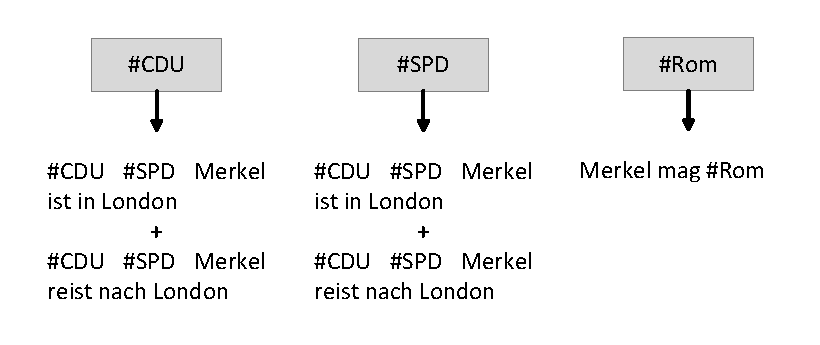
\includegraphics[scale=0.9]{./Bilder/Clustering/HashtagClusteringIdee.pdf}
\caption{Erzeugung eines jeweiligen virtuellen Dokuments zu einem Hashtag}
\label{fig:HashtagClusteringSchritt2}
\end{figure}
%
\item Entferne alle Hashtags, die weniger als $x$ Tweets enthalten. Verschiedene Werte für $x$ wurden ausprobiert und mit $x=15$ gute Ergebnisse erzielt. Dieser Korrekturschritt ist notwendig, damit seltene Hashtags aus der Analyse fallen. Enthält ein Hashtag beispielsweise nur zwei oder drei Tweets, tritt nach wie vor die Problematik der vorherigen Tweet-Analyse auf. Es lassen sich nur wenig aussagekräftige Merkmale ableiten. In Abbildung \ref{fig:HashtagClusteringSchritt2} würde zum Beispiel \glqq \#Rom\grqq{} mit $x=2$ entfernt werden.
%
\item Berechne die Merkmale für jeden Hashtag. Anders als bei der Tweet-Analyse, werden nun die Worthäufigkeiten erfasst.
Während ein Wort bei einem einzelnen Tweet in der Regel nur selten wiederholt wird, kann die Wiederholung bei einem virtuellen Dokument in anderen Größenordnungen auftreten. Daher lohnt es sich hier, als Merkmal die Worthäufigkeit und nicht mehr das bloße Auftreten eines Wortes zu erfassen. Tabelle \ref{fig:ClusterTab3} zeigt die Merkmale für die jeweiligen Hashtags aus dem obigen Beispiel, wobei keine Hashtags entfernt werden.
%
%

\begin{table}[ht]
\centering
\small
\begin{tabular}{cccccccccccc}
\toprule
 & \#CDU & \#SPD  & Merkel & ist & in & London & reist & nach & mag & \#Rom \\ 
\midrule
\#CDU & 2 & 2  & 2 & 1 & 1 & 2 & 1 & 1 & 0 & 0\\ 

\#SPD & 2 & 2  & 2 & 1 & 1 & 2 & 1 & 1 & 0 & 0\\ 

\#Rom & 0 & 0  & 1 & 0 & 0 & 0 & 0 & 0 & 1 & 1\\ 
\bottomrule 
\end{tabular} 
\caption{Quantitative Merkmale eines Hashtags: Worthäufigkeiten}
\label{fig:ClusterTab3}
\end{table}

%
%
\item Dividiere jedes Merkmal eines Hashtags durch die entsprechende Zeilensumme.
Die Zeilensumme stellt die Gesamtanzahl der Wörter eines Hashtags dar. Durch die Division der Häufigkeit eines Wortes durch die Gesamtanzahl ergibt sich ein relativer Anteil dieses Wortes an der Gesamtzahl der verwendeten Wörter. Im Beispiel ergibt sich somit für das Merkmal \glqq Merkel\grqq{} des Hashtags \glqq \#CDU\grqq{} der Wert $2/12$.

Diese Datenvorbereitung ist notwendig, da jedes virtuelle Dokument aus einer anderen Anzahl an Tweets gebildet wird. Ist zum Beispiel das Wort \glqq kerry\grqq{} in 20 von 40 Wörtern beim Hashtag \glqq \#merkel\grqq{} vorhanden und in 10 von 20 Wörtern beim Hashtag \glqq \#steinmeier\grqq{}, so unterscheiden sich beide Hashtags bei der absoluten Wortanzahl deutlich. Relativ gesehen tritt \glqq kerry\grqq{} aber bei beiden Hashtags in 50\% der Wörter auf. Beide Hashtags sind sich also ähnlicher.
%
%
\item Berechne die Distanzmatrix. Da es sich bei der Wortanzahl um ein quantitatives Merkmal handelt, lassen sich nun andere Distanzmaße verwenden. Hier wurde die euklidische Distanz als Metrik eingesetzt. Weitere Scrum-Iterationen sollten auch die Evaluierung anderer Metriken beinhalten. 
%
\item Führe einen Cluster-Algorithmus sowie eine multidimensionale Skalierung durch.
\end{enumerate}
Das beschriebene Vorgehen basiert auf \cite{TsurLittman}, ist aber mit Schritt~3~und~5 sowie mit der multidimensionalen Skalierung aus Schritt~7 entsprechend erweitert. 

In der praktischen Anwendung ergaben sich deutlich bessere Ergebnisse als bei der vorherigen Tweet-Analyse, da die Distanzen auf Grund der mehr zur Verfügung stehenden Informationen aussagekräftiger sind. So wurden zum Beispiel \glqq \#merkel\grqq{}, \glqq \#schumacher\grqq{} und \glqq \#ski\grqq{} (Stand: 12.03.2014, \glqq Alle Sprachen\grqq{}) in einem Cluster dicht aneinander dargestellt. Daraus ließ sich zum Beispiel mit dem News-Modul ableiten, dass viele Tweets den Skiunfall von Merkel und Schumacher behandeln. 

Schwierig ist jedoch die Interpretation im Frontend, warum zwei Hashtags in einem Cluster liegen. Künftige Scrum-Iterationen sollten daher im Frontend zum Beispiel eine Möglichkeit bieten, die Tweets zu zwei markierten Hashtags anzuzeigen. Damit lässt sich besser ein Gefühl vermitteln, wie das Ergebnis zustande gekommen ist.

%Um Hashtags gegenseitig nach ihrer Ähnlichkeit zu bewerten, ist es aber auch alternativ möglich, die \glqq Co-Occurence\grqq{} zwi\-schen zwei Hashtags zu zählen \cite{Antenucci}. Zwei Hashtags sind sich umso ähnlicher, je häufiger sie gemeinsam in einem Tweet auftreten.
%Diese Ähnlichkeitsanalyse ist ebenfalls implementiert worden, wird jedoch aus Laufzeitgründen nicht eingesetzt. 

%Erwin
\subsection{Verwendung der Hashtag-Cluster zur Tweet-Gruppierung} \label{subsec:ClusterTweetsWithHashtags}
Sind die Hashtag-Cluster aus einer Menge an Tweets berechnet, lassen sich nun im wei\-te\-ren Schritt die Tweet-Gruppen berechnen.
Dazu werden die Tweets, die das jeweilige virtuelle Dokument zu einem Hashtag bilden, in den gleichen Cluster eingeordnet wie der entsprechende Hashtag \cite{TsurLittman}. Angenommen, im obigen Beispiel erhält der Hashtag \glqq \#Rom\grqq{} die Cluster-Nummer 2. Alle Tweets, die im virtuellen Dokument von \glqq \#Rom\grqq{} liegen, erhalten somit ebenfalls die Cluster-Nummer 2. 

Ein Problem ist allerdings, dass ein Tweet durchaus in mehreren virtuellen Dokumenten enthalten sein kann, sofern mehrere Hashtags verwendet werden. Besitzen diese unterschiedliche Cluster-Zugehörigkeiten, ist eine 1:1-Zuordnung zwi\-schen Hashtag-Cluster und Tweet-Cluster nicht mehr möglich.

Daher wurde versucht, für jeden Tweet gemäß einer Distanzfunktion den nächsten Hash\-tag zu finden, Der Tweet erbt anschließend die Cluster-Nummer des Hashtags. Damit ist zwar eine eindeutige 1:1-Zuordnung möglich, aber es entsteht erneut das Problem, dass ein Tweet selbst zu wenig Merkmale enthält, um aussagekräftige Distanzen zu den Hashtags abzuleiten. 

Ein wei\-te\-res Problem des Ansatzes ist die Anforderung, 
Tweets durch die multidimensionale Skalierung in die 2D-Ebene 
einzubetten. Ein Tweet selbst erhält nur die 
Cluster-Zugehörigkeit des Hashtags, hat dadurch aber selbst keine Distanzen mehr zu anderen Tweets. 
Alle Tweets würden daher in einem Punkt dargestellt werden, 
dem Punkt, an dem theoretisch der Hashtag liegen würde. 
 Damit lassen sich aber die Distanzen 
zwi\-schen den Tweets nicht mehr interpretieren. Da dies nicht 
die ursprüngliche Motivation widerspiegelt, wurde das Ergebnis 
des hier geschilderten Ansatzes nicht im Frontend dargestellt, 
ist aber nach wie vor implementiert. 


%Wladimir, (Erwin)
\subsection{Cluster-Algorithmen} \label{subsec:ClusterAlgorithmen}

Bei der Wahl der Cluster-Algorithmen haben wir uns auf hierarchische Clusterverfahren 
beschränkt, die ohne Koordinaten der einzelnen Punkte auskommen. 
Der Grund dafür ist, dass man den einzelnen Entitäten, in unserem Fall
Tweets und Hashtags, zunächst keine Positionen zuordnen kann, d.\,h. die Tweets beziehungsweise Hashtags 
haben zwar Ähnlichkeiten zu einander, die man als Distanzen interpretieren kann, aber keine festgelegten 
Positionen in Raum. Es wäre zwar möglich gewesen, zuerst die multidimensionale Skalierung durchzuführen
und anschließend mit Hilfe der gewonnen Positionen zu clustern, aber es ist sehr unwahrscheinlich,
dass eine größere Anzahl an Entitäten mit geringen Fehlern in die 2D-Ebene eingebettet werden können.
Partitionierende Clusteringverfahren, wie $k$-Means \cite{Llo1982} kamen aus diesem Grund nicht in Frage.

Es sind zwei hierarchische Cluster"=Algorithmen implementiert worden, ein Single"=Linkage"=Algorithmus und ein
Complete"=Linkage"=Algorithmus. 
Durch die Implementierung beider Algorithmen ist es möglich, die Auswirkungen beider Ansätze auf das Ergebnis zu beobachten. Da Complete Linkage kompaktere
Cluster erzeugt, haben wir uns für diesen Algorithmus entschieden. Im Folgenden werden die 
beiden Cluster-Algorithmen einzeln vorgestellt.

%Erwin
\subsubsection{Single-Linkage-Algorithmus}
Die Cluster"=Analyse lässt sich auch als Graph-Problem darstellen, wobei die Knoten die zu gruppierenden Objekte darstellen (hier Tweets oder Hashtags). Außerdem handelt es sich um einen vollständigen Graphen, da alle möglichen Objektpaare aus der Distanzmatrix abgebildet werden. Die Kantenkosten sind die jeweiligen Distanzen aus der Distanzmatrix. 

Das Single"=Linkage"=Clustering stellt nun das gleiche Problem 
dar wie die Berechnung des minimalen Spannbaums (MST) durch 
den Kruskal-Algorithmus \cite{Kru1956}. Jede hinzugefügte 
Kante bei der MST-Berechnung stellt einen Fusionierungsschritt 
beim Clustern dar. Sollen beispielsweise $N$ Cluster berechnet 
werden, muss bei der Verwendung einer Union-Find-Datenstruktur 
abgebrochen werden, sobald $N$ Repräsentanten übrig sind.

Der Kruskal"=Algorithmus besitzt eine Laufzeit von $\mathcal{O}(E \log E)$, wobei $E$ die Kantenanzahl darstellt. Da hier ein vollständiger Graph abgearbeitet wird, gilt hier $E = M^2$ mit $M$ als die Anzahl der zu clusternden Entitäten (Knotenanzahl). Durch die Adaption des Kruskal"=Algorithmus besitzt der Single-Linkage-Algorithmus damit eine Laufzeit von $\mathcal{O}(M^2 \log M^2) = \mathcal{O}(M^2 \log M)$.


%Wladimir
\subsubsection{Complete-Linkage-Algorithmus}
Die Idee bei der Implementierung des Complete"=Linkage"=Algorithmus 
war, den naiven hierarchischen Algorithmus zu verwenden, 
an die eigenen Bedürfnisse anzupassen und anschließend die
Laufzeit zu verbessern.

Sei $S=\left\lbrace t_1, \dots, t_M \right\rbrace$ die Menge der zu clusternden Entitäten, 
$d:S^2 \rightarrow \mathbb{R}$ eine Distanzfunktion und $N$ die maximale Anzahl der Cluster,
dann lässt sich der implementierte hierarchische Algorithmus zu Algorithmus \ref{alg:genericHierarchicalAlgorithm}
zusammenfassen.

\begin{algorithm}
 \caption{Generischer hierarchischer Algorithmus}\label{alg:genericHierarchicalAlgorithm}
\begin{algorithmic}[1]
\Statex \textbf{Eingabe:} Menge der Entitäten $\left\lbrace t_1, \dots, t_M\right\rbrace$, $N$ die maximale Anzahl der Cluster
\Statex \textbf{Ausgabe:} Menge der Cluster $\mathcal{C}$
\State $\mathcal{C} = \left\lbrace \left\lbrace t_1 \right\rbrace, \left\lbrace t_2 \right\rbrace, \dots, \left\lbrace t_M \right\rbrace  \right\rbrace$
\For{$(i = 1; i < M\ \textbf{and}\ |\mathcal{C}| > N ; i++)$}
\State $(c_i, c_j) = \operatorname*{arg\,min}\limits_{c_i,c_j \in \mathcal{C},\ i \not= j}  d(c_i, c_j)$
\State $\mathcal{C} = \left( \mathcal{C}\backslash{\left\lbrace c_i,\ c_j \right\rbrace}\right) \cup \left\lbrace c_i \cup c_j \right\rbrace $
\EndFor
\end{algorithmic}
\end{algorithm}

Die Wahl der Funktion $d$ bestimmt das Verhalten des Algorithmus. Wir haben $d$ entsprechend 
dem Complete-Linkage wie folgt gewählt:
\begin{align}
 d(c_i,c_j) := \max{\left\lbrace \delta(t_i,t_j)\ |\ t_i\in c_i, t_j\in c_j \right\rbrace}. \notag
\end{align}
Dabei stellt der Ausdruck $\delta(t_i,t_j)$ die aus der Distanzmatrix stammenden Unähnlichkeiten 
zwi\-schen den Tweets beziehungsweise Hashtags dar.

Bei der naiven Implementierung des obigen Algorithmus beträgt die Laufzeit $\mathcal{O}(M^3)$. Um die Laufzeit auf
$\mathcal{O}(M^2 \log M)$ zu verbessern, haben wir den Algorithmus so mo\-di\-fi\-ziert, dass zur Verwaltung der
Unähnlichkeiten ein Heap verwendet wird. Insgesamt müssen durch den Heap $\frac{M^2}{2}-M \in \mathcal{O}(M^2)$ Werte
verwalten werden. Es werden aber auch maximal $\frac{M^2}{2}-M$ Werte wieder aus dem Heap entfernt, falls $N = 1$ gilt (\textit{worst case}). Insgesamt wird
also zum Erzeugen und Verwalten des Heaps $\mathcal{O}(M^2 + M^2 \log M^2) = \mathcal{O}(M^2 \log M)$ Zeit
benötigt, was auch der Laufzeit von dem implementierten Algorithmus entspricht.

%Wladimir
\subsection{Multidimensionale Skalierung} \label{subsec:MDS}
Das Ziel der multidimensionalen Skalierung ist es, die gegebenen Objekte im Raum oder in der Ebene anzuordnen. 
Dabei sollen die Abstände der Objekte zueinander nach der multidimensionalen Skalierung ihre
Unähnlichkeiten möglichst gut wiedergeben. Dadurch ist es möglich, Objekte, die eigentlich keine Punkte 
im euklidischen Raum sind, als solche zu interpretieren und so Informationen anschaulicher darzustellen oder
neue Zusammenhänge zu entdecken. In der Abbildung \ref{img:MDSAutoMarkenBeispiel} ist die Anwendung
der multidimensionalen Skalierung auf eine Umfrage zu unterschiedlichen Automarken dargestellt. 
Bei der Umfrage haben die Befragten angegeben, wie ähnlich die betroffenen Automarken zueinander sind. Man kann
 sehen, dass bei der geeigneten Wahl von Parametern und Verfahren die Punkte in bestimmten Teilen der Ebene
liegen, die charakteristisch für sie sind, zum Beispiel liegen die Sportwagenhersteller nah bei einander.

\begin{figure}
 \centering
 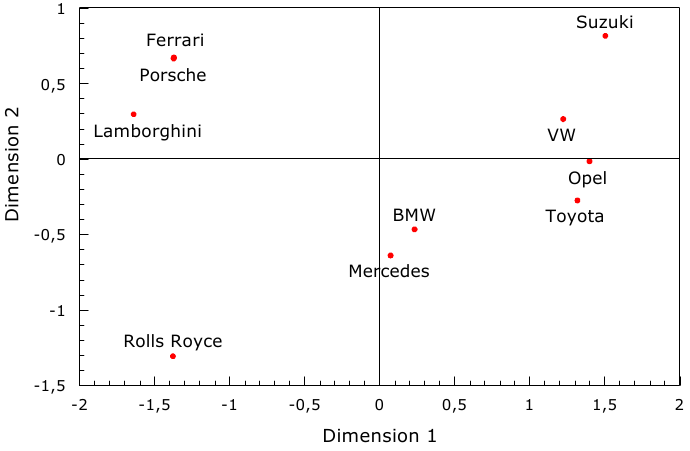
\includegraphics[width=0.8\textwidth]{./Bilder/Clustering/mittlereunaenlichkeitenderautomarken.png}
\caption{Multidimensionale Skalierung angewandt auf eine Umfrage zu Unterschieden 
zwi\-schen bekannten Automarken. Bild entnommen aus \cite{Kappelhoff2001}.}\label{img:MDSAutoMarkenBeispiel}
\end{figure} 

Für unser Projekt haben wir zwei Verfahren zur multidimensionale Skalierung implementiert: \textit{classical scaling} und den Smacof-Algorithmus.
Beide Verfahren sind in \cite{BorgGroenen2005} ausführlich beschrieben. \textit{Classical scaling} ist ein Verfahren, das 
analytisch die multidimensionale Skalierung berechnet, wohingegen der Smacof-Algorithmus ein iteratives Verfahren ist
und wesentlich mehr Parameter bietet. In den folgenden Kapiteln werden die beiden Verfahren kurz vorgestellt. 
Für eine ausführliche Beschreibung der vorgestellten Verfahren verweisen wir auf \cite{BorgGroenen2005}.

%Wladimir
\subsubsection{Classical Scaling}
\textit{Classical scaling} berechnet analytisch zu gegebenen Unähnlichkeiten, die als Distanzen interpretiert werden, eine passende Punktemenge.
Die Abstände der Punkte untereinander entsprechen den gegeben Distanzen, wenn die Dimension des Raumes, in dem die Punkte liegen,
hoch genug ist. 
Der Sinn und Zweck der multidimensionalen Skalierung ist es, die Dimension, in der die Punkte liegen, 
gering zu halten. Damit lassen sich diese grafisch darstellen, wenn die Dimension kleiner als vier ist.
Aus diesem Grund können die berechneten Punkte 
die vorgegebenen Distanzen nur approximieren. Wobei die Approximation schlechter wird, wenn die Anzahl der Dimensionen sinkt.

Sei $\mathbf{\Delta} \in \mathbb{R}^{n\times n}$ die Matrix mit den Distanzen der $n$ Punkte. Ziel ist es eine (von vielen) 
Punktekonstellation zu finden, die diese Matrix erzeugt und eine Approximation davon in einem niedrigdimensionalen Raum zu nehmen.
Das Vorgehen bei \textit{classical scaling} lässt sich dann wie folgt zusammenfassen:
\begin{enumerate}
 \item Berechne $\mathbf{\Delta}^{(2)}=$ Quadrate der Einträge von $\mathbf{\Delta}$.
 \item Berechne $-\tfrac{1}{2}\mathbf{C}_n\mathbf{\Delta}^{(2)}\mathbf{C}_n =: \mathbf{XX}^T$, $\mathbf{C}_n=\mathbf{I}_n-\tfrac{1}{n}\mathbf{1}_n$, 
 $\mathbf{I}_n$ ist die $n$-dimensionale Einheitsmatrix und $\mathbf{1}_n$
 ist die $n$-dimensionale Matrix mit Einsen.
 \item Berechne die Eigenwertdekomposition $\mathbf{XX}^T = \mathbf{Q\Lambda Q}^T = \mathbf{Q\Lambda}^{1/2}(\mathbf{Q\Lambda}^{1/2})^T$, 
 $\mathbf{\Lambda}^{1/2}$ ist Diagonalmatrix mit Quadratwurzeln der Elemente aus $\mathbf{\Lambda}$.
 \item Berechne für ein gewünschtes $d\in \left\lbrace 1,\ 2,\ 3 \right\rbrace$: 
 $\mathbf{X}_d= \mathbf{Q}_d\mathbf{\Lambda}^{1/2}_d$, dabei ist
 $\mathbf{\Lambda}^{1/2}_d$ die Matrix mit den Quadratwurzeln der $d$ größten positiven Eigenwerte und $\mathbf{Q}_d$ ist die Matrix mit 
 entsprechenden Eigenvektoren.
\end{enumerate}

Erklärung der Schritte:
\begin{enumerate}
 \item Nimmt man an, dass man Punkte hat, die die Distanzen aus der Matrix $\mathbf{\Delta}$ erzeugen und die 
 Koordinaten dieser Punkte stehen in der Matrix $\mathbf{X}$ (Zeilenweise),
  dann kann man den quadrierten  euklidische Abstand zweier Vektoren, wie folgt berechnen:
  \begin{align}
   d^2_{ij} = \sum_{k=1}^{n}(x_{ik}-x_{jk})^2 = \sum_{k=1}^{n} (x_{ik}^2 -2x_{ik}x_{jk}+x_{jk}^2). \label{eq:qudeukldist}
  \end{align}
  Berechnet man die quadrierten  euklidischen Abstände für alle Paare, erhält man die Einträge der Matrix $\mathbf{\Delta}^{(2)}$. Man rechnet
  mit den quadrierten Abständen, weil man dadurch die Summe aus \eqref{eq:qudeukldist} in mehrere Summen aufteilen kann. Dadurch kann man die 
  Matrix $\mathbf{\Delta}^{(2)}$ wie folgt schreiben:
  \begin{align*}
   \mathbf{\Delta}^{(2)}(\mathbf{X}) = \mathbf{c}\mathbf{1}^T + \mathbf{1}\mathbf{c}^T - 2\mathbf{X}\mathbf{X}^T,
  \end{align*}
wobei $\mathbf{c}$ ein Vektor mit den Diagonalelementen aus $\mathbf{X}\mathbf{X}^T$ und $\mathbf{1}\in \mathbb{R}^n$ ist ein Vektor mit Einsen sind.
Dieser Zusammenhang ist der Grund für die Berechnung von $\mathbf{\Delta}^{(2)}$.
\item In diesem Schritt wird die Matrix $\mathbf{\Delta}^{(2)}$ beidseitig mit der Matrix $\mathbf{C}_n$ multipliziert ($\mathbf{C}_n$, wie oben in Schritt 2).
Matrix $\mathbf{C}_n$ ist die Zentrierungsmatrix, d.\,h. eine Anwendung auf einen Vektor bewirkt das Subtrahieren des Mittelwertes seiner Einträge von jedem Eintrag, z.\,B.
\begin{align*}
 \mathbf{C}_2 \left( \begin{matrix}
 2 \\
 4 
\end{matrix} \right)
=
\left( \begin{matrix}
 \frac{1}{2} & -\frac{1}{2} \\
 -\frac{1}{2}& \frac{1}{2} 
\end{matrix} \right) \left( \begin{matrix}
 2 \\
 4 
\end{matrix} \right)
=
\left(
\begin{matrix}
 -1 \\
 1 
\end{matrix}
\right).
\end{align*}
Wichtige Spezialfälle sind: 
\begin{itemize}
 \item Zentrierung eines Vektors, der nur Einsen enthält und
 \item Zentrierung  eines bereits zentrierten Vektors.
\end{itemize}
Im ersten Fall erhält man den Nullvektor, weil der Mittelwert eines Vektors nur mit Einsen immer den Wert 1 hat. Im zweiten Fall bewirkt die Zentrierung nichts, da der 
Vektor bereits zentriert ist. Multipliziert man $\mathbf{\Delta}^{(2)}$ beidseitig mit $\mathbf{C}_n$, ergibt sich:
\begin{align*}
 \mathbf{C}_n\mathbf{\Delta}^{(2)}\mathbf{C}_n &= \mathbf{C}_n\left(\mathbf{c}\mathbf{1}^T + \mathbf{1}\mathbf{c}^T - 2\mathbf{X}\mathbf{X^T} \right)\mathbf{C}_n \\
                                               &= \mathbf{C}_n\mathbf{c}\mathbf{1}^T\mathbf{C}_n + \mathbf{C}_n\mathbf{1}\mathbf{c}^T\mathbf{C}_n - 2\mathbf{C}_n\mathbf{X}\mathbf{X^T}\mathbf{C}_n \\
                                               &= \mathbf{C}_n\mathbf{c}\mathbf{0}^T + \mathbf{0}\mathbf{c}^T\mathbf{C}_n - 2\mathbf{C}_n\mathbf{X}\mathbf{X^T}\mathbf{C}_n \\
                                               &=   \underbrace{- 2\mathbf{C}_n\mathbf{X}\mathbf{X^T}\mathbf{C}_n}_{\text{X ist zentriert}} \\
                                               &= -2 \mathbf{X}\mathbf{X^T}.
\end{align*}
Im letzten Schritt der Rechnung nimmt man an, dass die Matrix $\mathbf{X}$ zentriert ist. Das ist keine Einschränkung, weil man eine beliebige Lösung sucht. Außerdem
lässt sich die Lösung durch eine Translation anpassen, sodass die Distanzen zwischen den Punkten unverändert bleiben.

\item Um aus der Matrix $\mathbf{X}\mathbf{X}^T$ die Matrix $\mathbf{X}$ zu extrahieren, benutzt man die Eigenwertdekomposition. Dabei macht man die Annahme, dass 
die Eigenwerte nicht negativ sind.
\item Um eine Approximation von $\mathbf{X}$ für die gewünschte Dimension zu erhalten, benutzt man die größten Eigenwerte und die entsprechenden Eigenvektoren.
\end{enumerate}


Es ist wichtig anzumerken, dass \textit{classical scaling} mit der Hauptkomponentenanalyse
\cite{jolliffe2002principal} eng verwandt ist. Der Unterschied ist hilfreich für das Verständnis des Vorgehens beim \textit{classical scaling}. Bei
der Hauptkomponentenanalyse möchte man die Dimension der betrachteten Punkte reduzieren, während es bei \textit{classical scaling} zusätzlich
darum geht, die Punkte selbst zu finden.

%Wladimir
\subsubsection{Smacof-Algorithmus}
Die Idee beim Smacof-Algorithmus ist, eine gewählte Funktion $\sigma_\mathbf{\Delta}:\mathbb{R}^{n\times d} \rightarrow \mathbb{R}$ zu mi\-ni\-mie\-ren. Die
Funktion $\sigma_\mathbf{\Delta}$ ist dabei ein Maß für den Fehler, der bei der Wahl der $n$ Punkte im $d$-dimensionalen Raum entsteht. Wir haben
in unserer Implementierung $\sigma_\mathbf{\Delta}$ wie folgt gewählt:
\begin{align*}
 \sigma_\mathbf{\Delta}(\mathbf{X}) = \sum_{i=1}^n \sum_{j=i+1}^n (d(\mathbf{x}_i, \mathbf{x}_j) - \delta_{ij})^2.
\end{align*}
Dabei ist $\mathbf{x}_i$ die $i$-te Zeile von $\mathbf{X}$, $d(\mathbf{x}_i, \mathbf{x}_j) = \Vert \mathbf{x}_i^T - \mathbf{x}_j^T  \Vert$,
$\mathbf{\Delta}$ ist die Unähnlichkeitsmatrix (die Einträge an der Position $ij$ geben an, wie unähnlich Entität i zur Entität j ist) und $\delta_{ij}$'s sind die Einträge von $\mathbf{\Delta}$. Die Lösung soll also eine 
Punktmenge sein, sodass die Summe der Quadrate der Differenzen zwischen den resultierenden Abständen und Unähnlichkeiten minimiert wird.

\begin{figure}[ht]
   \centering
   \def\maxW{4.26}
\begin{tikzpicture}[scale=\textwidth/2.6cm, background rectangle/.style={draw=black, thick, fill=yellow!10,},show background rectangle]
\def\marRad{0.2}
\definecolor{color0}{rgb}{0.78,0.89,0.11}
\definecolor{color1}{rgb}{0.10,1.00,0.52}
\definecolor{color2}{rgb}{0.09,0.32,0.64}
\definecolor{color3}{rgb}{0.70,0.69,0.42}
\definecolor{color4}{rgb}{0.36,0.70,0.25}
\definecolor{color5}{rgb}{0.91,0.34,0.56}
\definecolor{color6}{rgb}{0.76,0.33,0.65}
\definecolor{color7}{rgb}{0.06,0.22,0.62}
\definecolor{color8}{rgb}{0.45,0.68,0.87}
\definecolor{color9}{rgb}{0.03,0.89,0.67}
\path[fill=color0,draw=color0,mark size=\marRad, mark=*] plot coordinates {(0.44, -0.03)};
\path[fill=color0,draw=color0,mark size=\marRad, mark=*] plot coordinates {(0.43, 0.01)};
\path[fill=color0,draw=color0,mark size=\marRad, mark=*] plot coordinates {(0.43, -0.05)};
\path[fill=color0,draw=color0,mark size=\marRad, mark=*] plot coordinates {(0.48, 0.00)};
\path[fill=color0,draw=color0,mark size=\marRad, mark=*] plot coordinates {(0.44, -0.01)};
\path[fill=color0,draw=color0,mark size=\marRad, mark=*] plot coordinates {(0.41, 0.00)};
\path[fill=color0,draw=color0,mark size=\marRad, mark=*] plot coordinates {(0.43, -0.01)};
\path[fill=color0,draw=color0,mark size=\marRad, mark=*] plot coordinates {(0.46, -0.00)};
\path[fill=color0,draw=color0,mark size=\marRad, mark=*] plot coordinates {(0.45, -0.00)};
\path[fill=color0,draw=color0,mark size=\marRad, mark=*] plot coordinates {(0.41, -0.02)};
\path[fill=color0,draw=color0,mark size=\marRad, mark=*] plot coordinates {(0.47, 0.03)};
\path[fill=color0,draw=color0,mark size=\marRad, mark=*] plot coordinates {(0.46, -0.00)};
\path[fill=color0,draw=color0,mark size=\marRad, mark=*] plot coordinates {(0.42, 0.02)};
\path[fill=color0,draw=color0,mark size=\marRad, mark=*] plot coordinates {(0.38, -0.00)};
\path[fill=color0,draw=color0,mark size=\marRad, mark=*] plot coordinates {(0.41, -0.00)};
\path[fill=color0,draw=color0,mark size=\marRad, mark=*] plot coordinates {(0.43, 0.01)};
\path[fill=color0,draw=color0,mark size=\marRad, mark=*] plot coordinates {(0.43, -0.06)};
\path[fill=color0,draw=color0,mark size=\marRad, mark=*] plot coordinates {(0.45, 0.01)};
\path[fill=color0,draw=color0,mark size=\marRad, mark=*] plot coordinates {(0.40, -0.03)};
\path[fill=color0,draw=color0,mark size=\marRad, mark=*] plot coordinates {(0.44, -0.01)};
\path[fill=color0,draw=color0,mark size=\marRad, mark=*] plot coordinates {(0.45, 0.07)};
\path[fill=color0,draw=color0,mark size=\marRad, mark=*] plot coordinates {(0.46, -0.05)};
\path[fill=color0,draw=color0,mark size=\marRad, mark=*] plot coordinates {(0.46, 0.04)};
\path[fill=color0,draw=color0,mark size=\marRad, mark=*] plot coordinates {(0.38, -0.00)};
\path[fill=color0,draw=color0,mark size=\marRad, mark=*] plot coordinates {(0.47, 0.04)};
\path[fill=color0,draw=color0,mark size=\marRad, mark=*] plot coordinates {(0.45, -0.01)};
\path[fill=color0,draw=color0,mark size=\marRad, mark=*] plot coordinates {(0.42, -0.02)};
\path[fill=color0,draw=color0,mark size=\marRad, mark=*] plot coordinates {(0.42, 0.03)};
\path[fill=color0,draw=color0,mark size=\marRad, mark=*] plot coordinates {(0.43, 0.06)};
\path[fill=color0,draw=color0,mark size=\marRad, mark=*] plot coordinates {(0.44, -0.06)};
\path[fill=color0,draw=color0,mark size=\marRad, mark=*] plot coordinates {(0.47, 0.01)};
\path[fill=color0,draw=color0,mark size=\marRad, mark=*] plot coordinates {(0.48, -0.05)};
\path[fill=color0,draw=color0,mark size=\marRad, mark=*] plot coordinates {(0.49, 0.02)};
\path[fill=color0,draw=color0,mark size=\marRad, mark=*] plot coordinates {(0.46, -0.01)};
\path[fill=color0,draw=color0,mark size=\marRad, mark=*] plot coordinates {(0.42, 0.04)};
\path[fill=color0,draw=color0,mark size=\marRad, mark=*] plot coordinates {(0.44, 0.00)};
\path[fill=color0,draw=color0,mark size=\marRad, mark=*] plot coordinates {(0.42, 0.01)};
\path[fill=color0,draw=color0,mark size=\marRad, mark=*] plot coordinates {(0.41, -0.02)};
\path[fill=color0,draw=color0,mark size=\marRad, mark=*] plot coordinates {(0.48, 0.03)};
\path[fill=color0,draw=color0,mark size=\marRad, mark=*] plot coordinates {(0.42, 0.06)};
\path[fill=color0,draw=color0,mark size=\marRad, mark=*] plot coordinates {(0.40, -0.05)};
\path[fill=color0,draw=color0,mark size=\marRad, mark=*] plot coordinates {(0.41, 0.04)};
\path[fill=color0,draw=color0,mark size=\marRad, mark=*] plot coordinates {(0.44, -0.03)};
\path[fill=color0,draw=color0,mark size=\marRad, mark=*] plot coordinates {(0.45, -0.02)};
\path[fill=color0,draw=color0,mark size=\marRad, mark=*] plot coordinates {(0.41, -0.00)};
\path[fill=color0,draw=color0,mark size=\marRad, mark=*] plot coordinates {(0.44, 0.00)};
\path[fill=color0,draw=color0,mark size=\marRad, mark=*] plot coordinates {(0.40, 0.02)};
\path[fill=color0,draw=color0,mark size=\marRad, mark=*] plot coordinates {(0.43, 0.05)};
\path[fill=color0,draw=color0,mark size=\marRad, mark=*] plot coordinates {(0.51, -0.01)};
\path[fill=color0,draw=color0,mark size=\marRad, mark=*] plot coordinates {(0.46, 0.03)};
\path[fill=color0,draw=color0,mark size=\marRad, mark=*] plot coordinates {(0.43, -0.02)};
\path[fill=color0,draw=color0,mark size=\marRad, mark=*] plot coordinates {(0.50, 0.03)};
\path[fill=color0,draw=color0,mark size=\marRad, mark=*] plot coordinates {(0.44, 0.02)};
\path[fill=color0,draw=color0,mark size=\marRad, mark=*] plot coordinates {(0.48, -0.04)};
\path[fill=color0,draw=color0,mark size=\marRad, mark=*] plot coordinates {(0.43, 0.01)};
\path[fill=color0,draw=color0,mark size=\marRad, mark=*] plot coordinates {(0.49, 0.01)};
\path[fill=color0,draw=color0,mark size=\marRad, mark=*] plot coordinates {(0.44, -0.02)};
\path[fill=color0,draw=color0,mark size=\marRad, mark=*] plot coordinates {(0.43, 0.01)};
\path[fill=color0,draw=color0,mark size=\marRad, mark=*] plot coordinates {(0.46, -0.03)};
\path[fill=color0,draw=color0,mark size=\marRad, mark=*] plot coordinates {(0.44, 0.00)};
\path[fill=color0,draw=color0,mark size=\marRad, mark=*] plot coordinates {(0.42, -0.01)};
\path[fill=color0,draw=color0,mark size=\marRad, mark=*] plot coordinates {(0.49, -0.02)};
\path[fill=color0,draw=color0,mark size=\marRad, mark=*] plot coordinates {(0.44, -0.00)};
\path[fill=color0,draw=color0,mark size=\marRad, mark=*] plot coordinates {(0.45, -0.01)};
\path[fill=color0,draw=color0,mark size=\marRad, mark=*] plot coordinates {(0.50, 0.04)};
\path[fill=color0,draw=color0,mark size=\marRad, mark=*] plot coordinates {(0.44, 0.00)};
\path[fill=color0,draw=color0,mark size=\marRad, mark=*] plot coordinates {(0.45, 0.00)};
\path[fill=color0,draw=color0,mark size=\marRad, mark=*] plot coordinates {(0.39, 0.01)};
\path[fill=color0,draw=color0,mark size=\marRad, mark=*] plot coordinates {(0.47, -0.00)};
\path[fill=color0,draw=color0,mark size=\marRad, mark=*] plot coordinates {(0.45, -0.01)};
\path[fill=color0,draw=color0,mark size=\marRad, mark=*] plot coordinates {(0.44, 0.01)};
\path[fill=color0,draw=color0,mark size=\marRad, mark=*] plot coordinates {(0.44, -0.01)};
\path[fill=color0,draw=color0,mark size=\marRad, mark=*] plot coordinates {(0.45, -0.00)};
\path[fill=color0,draw=color0,mark size=\marRad, mark=*] plot coordinates {(0.46, 0.06)};
\path[fill=color0,draw=color0,mark size=\marRad, mark=*] plot coordinates {(0.44, 0.04)};
\path[fill=color0,draw=color0,mark size=\marRad, mark=*] plot coordinates {(0.40, -0.00)};
\path[fill=color0,draw=color0,mark size=\marRad, mark=*] plot coordinates {(0.48, 0.01)};
\path[fill=color0,draw=color0,mark size=\marRad, mark=*] plot coordinates {(0.40, 0.04)};
\path[fill=color0,draw=color0,mark size=\marRad, mark=*] plot coordinates {(0.45, -0.00)};
\path[fill=color0,draw=color0,mark size=\marRad, mark=*] plot coordinates {(0.46, 0.01)};
\path[fill=color0,draw=color0,mark size=\marRad, mark=*] plot coordinates {(0.45, 0.04)};
\path[fill=color0,draw=color0,mark size=\marRad, mark=*] plot coordinates {(0.43, 0.06)};
\path[fill=color0,draw=color0,mark size=\marRad, mark=*] plot coordinates {(0.40, -0.01)};
\path[fill=color0,draw=color0,mark size=\marRad, mark=*] plot coordinates {(0.45, 0.02)};
\path[fill=color0,draw=color0,mark size=\marRad, mark=*] plot coordinates {(0.46, 0.00)};
\path[fill=color0,draw=color0,mark size=\marRad, mark=*] plot coordinates {(0.47, 0.02)};
\path[fill=color0,draw=color0,mark size=\marRad, mark=*] plot coordinates {(0.45, 0.00)};
\path[fill=color0,draw=color0,mark size=\marRad, mark=*] plot coordinates {(0.49, -0.04)};
\path[fill=color0,draw=color0,mark size=\marRad, mark=*] plot coordinates {(0.45, -0.02)};
\path[fill=color0,draw=color0,mark size=\marRad, mark=*] plot coordinates {(0.48, 0.04)};
\path[fill=color0,draw=color0,mark size=\marRad, mark=*] plot coordinates {(0.44, 0.00)};
\path[fill=color0,draw=color0,mark size=\marRad, mark=*] plot coordinates {(0.44, 0.01)};
\path[fill=color0,draw=color0,mark size=\marRad, mark=*] plot coordinates {(0.46, 0.02)};
\path[fill=color0,draw=color0,mark size=\marRad, mark=*] plot coordinates {(0.40, -0.01)};
\path[fill=color0,draw=color0,mark size=\marRad, mark=*] plot coordinates {(0.45, 0.01)};
\path[fill=color0,draw=color0,mark size=\marRad, mark=*] plot coordinates {(0.44, -0.00)};
\path[fill=color0,draw=color0,mark size=\marRad, mark=*] plot coordinates {(0.43, -0.01)};
\path[fill=color0,draw=color0,mark size=\marRad, mark=*] plot coordinates {(0.49, 0.03)};
\path[fill=color0,draw=color0,mark size=\marRad, mark=*] plot coordinates {(0.42, 0.03)};
\path[fill=color0,draw=color0,mark size=\marRad, mark=*] plot coordinates {(0.48, -0.03)};
\path[fill=color0,draw=color0,mark size=\marRad, mark=*] plot coordinates {(0.44, -0.00)};
\path[fill=color0,draw=color0,mark size=\marRad, mark=*] plot coordinates {(0.45, 0.01)};
\path[fill=color0,draw=color0,mark size=\marRad, mark=*] plot coordinates {(0.44, -0.06)};
\path[fill=color0,draw=color0,mark size=\marRad, mark=*] plot coordinates {(0.42, 0.02)};
\path[fill=color0,draw=color0,mark size=\marRad, mark=*] plot coordinates {(0.44, -0.04)};
\path[fill=color0,draw=color0,mark size=\marRad, mark=*] plot coordinates {(0.49, -0.01)};
\path[fill=color0,draw=color0,mark size=\marRad, mark=*] plot coordinates {(0.43, -0.00)};
\path[fill=color0,draw=color0,mark size=\marRad, mark=*] plot coordinates {(0.44, -0.05)};
\path[fill=color0,draw=color0,mark size=\marRad, mark=*] plot coordinates {(0.47, 0.01)};
\path[fill=color0,draw=color0,mark size=\marRad, mark=*] plot coordinates {(0.46, -0.03)};
\path[fill=color0,draw=color0,mark size=\marRad, mark=*] plot coordinates {(0.41, -0.04)};
\path[fill=color0,draw=color0,mark size=\marRad, mark=*] plot coordinates {(0.41, 0.05)};
\path[fill=color0,draw=color0,mark size=\marRad, mark=*] plot coordinates {(0.42, -0.05)};
\path[fill=color0,draw=color0,mark size=\marRad, mark=*] plot coordinates {(0.48, -0.04)};
\path[fill=color0,draw=color0,mark size=\marRad, mark=*] plot coordinates {(0.42, -0.00)};
\path[fill=color0,draw=color0,mark size=\marRad, mark=*] plot coordinates {(0.46, 0.00)};
\path[fill=color0,draw=color0,mark size=\marRad, mark=*] plot coordinates {(0.44, 0.01)};
\path[fill=color0,draw=color0,mark size=\marRad, mark=*] plot coordinates {(0.43, 0.04)};
\path[fill=color0,draw=color0,mark size=\marRad, mark=*] plot coordinates {(0.45, 0.03)};
\path[fill=color0,draw=color0,mark size=\marRad, mark=*] plot coordinates {(0.47, 0.02)};
\path[fill=color0,draw=color0,mark size=\marRad, mark=*] plot coordinates {(0.46, -0.06)};
\path[fill=color0,draw=color0,mark size=\marRad, mark=*] plot coordinates {(0.46, -0.01)};
\path[fill=color0,draw=color0,mark size=\marRad, mark=*] plot coordinates {(0.43, 0.03)};
\path[fill=color0,draw=color0,mark size=\marRad, mark=*] plot coordinates {(0.46, -0.03)};
\path[fill=color0,draw=color0,mark size=\marRad, mark=*] plot coordinates {(0.43, 0.05)};
\path[fill=color0,draw=color0,mark size=\marRad, mark=*] plot coordinates {(0.46, 0.04)};
\path[fill=color0,draw=color0,mark size=\marRad, mark=*] plot coordinates {(0.46, 0.04)};
\path[fill=color0,draw=color0,mark size=\marRad, mark=*] plot coordinates {(0.39, 0.01)};
\path[fill=color0,draw=color0,mark size=\marRad, mark=*] plot coordinates {(0.46, -0.03)};
\path[fill=color0,draw=color0,mark size=\marRad, mark=*] plot coordinates {(0.46, 0.02)};
\path[fill=color0,draw=color0,mark size=\marRad, mark=*] plot coordinates {(0.45, 0.00)};
\path[fill=color0,draw=color0,mark size=\marRad, mark=*] plot coordinates {(0.48, -0.03)};
\path[fill=color0,draw=color0,mark size=\marRad, mark=*] plot coordinates {(0.45, 0.03)};
\path[fill=color0,draw=color0,mark size=\marRad, mark=*] plot coordinates {(0.43, -0.01)};
\path[fill=color0,draw=color0,mark size=\marRad, mark=*] plot coordinates {(0.45, 0.00)};
\path[fill=color0,draw=color0,mark size=\marRad, mark=*] plot coordinates {(0.44, -0.05)};
\path[fill=color0,draw=color0,mark size=\marRad, mark=*] plot coordinates {(0.45, 0.01)};
\path[fill=color0,draw=color0,mark size=\marRad, mark=*] plot coordinates {(0.44, -0.01)};
\path[fill=color0,draw=color0,mark size=\marRad, mark=*] plot coordinates {(0.45, 0.02)};
\path[fill=color0,draw=color0,mark size=\marRad, mark=*] plot coordinates {(0.46, 0.01)};
\path[fill=color0,draw=color0,mark size=\marRad, mark=*] plot coordinates {(0.44, -0.01)};
\path[fill=color0,draw=color0,mark size=\marRad, mark=*] plot coordinates {(0.48, 0.01)};
\path[fill=color0,draw=color0,mark size=\marRad, mark=*] plot coordinates {(0.42, 0.01)};
\path[fill=color0,draw=color0,mark size=\marRad, mark=*] plot coordinates {(0.49, 0.03)};
\path[fill=color0,draw=color0,mark size=\marRad, mark=*] plot coordinates {(0.39, -0.02)};
\path[fill=color0,draw=color0,mark size=\marRad, mark=*] plot coordinates {(0.46, -0.05)};
\path[fill=color0,draw=color0,mark size=\marRad, mark=*] plot coordinates {(0.45, -0.06)};
\path[fill=color0,draw=color0,mark size=\marRad, mark=*] plot coordinates {(0.40, -0.03)};
\path[fill=color0,draw=color0,mark size=\marRad, mark=*] plot coordinates {(0.44, -0.07)};
\path[fill=color0,draw=color0,mark size=\marRad, mark=*] plot coordinates {(0.49, 0.03)};
\path[fill=color0,draw=color0,mark size=\marRad, mark=*] plot coordinates {(0.45, -0.05)};
\path[fill=color0,draw=color0,mark size=\marRad, mark=*] plot coordinates {(0.44, -0.01)};
\path[fill=color0,draw=color0,mark size=\marRad, mark=*] plot coordinates {(0.48, 0.02)};
\path[fill=color0,draw=color0,mark size=\marRad, mark=*] plot coordinates {(0.45, 0.05)};
\path[fill=color0,draw=color0,mark size=\marRad, mark=*] plot coordinates {(0.47, 0.03)};
\path[fill=color0,draw=color0,mark size=\marRad, mark=*] plot coordinates {(0.42, 0.06)};
\path[fill=color0,draw=color0,mark size=\marRad, mark=*] plot coordinates {(0.48, 0.01)};
\path[fill=color0,draw=color0,mark size=\marRad, mark=*] plot coordinates {(0.47, -0.02)};
\path[fill=color0,draw=color0,mark size=\marRad, mark=*] plot coordinates {(0.43, -0.00)};
\path[fill=color0,draw=color0,mark size=\marRad, mark=*] plot coordinates {(0.46, 0.00)};
\path[fill=color0,draw=color0,mark size=\marRad, mark=*] plot coordinates {(0.45, -0.03)};
\path[fill=color0,draw=color0,mark size=\marRad, mark=*] plot coordinates {(0.43, 0.02)};
\path[fill=color0,draw=color0,mark size=\marRad, mark=*] plot coordinates {(0.43, -0.06)};
\path[fill=color0,draw=color0,mark size=\marRad, mark=*] plot coordinates {(0.46, -0.01)};
\path[fill=color0,draw=color0,mark size=\marRad, mark=*] plot coordinates {(0.45, 0.03)};
\path[fill=color0,draw=color0,mark size=\marRad, mark=*] plot coordinates {(0.46, 0.05)};
\path[fill=color0,draw=color0,mark size=\marRad, mark=*] plot coordinates {(0.46, 0.03)};
\path[fill=color0,draw=color0,mark size=\marRad, mark=*] plot coordinates {(0.47, 0.01)};
\path[fill=color0,draw=color0,mark size=\marRad, mark=*] plot coordinates {(0.44, -0.00)};
\path[fill=color0,draw=color0,mark size=\marRad, mark=*] plot coordinates {(0.44, 0.01)};
\path[fill=color0,draw=color0,mark size=\marRad, mark=*] plot coordinates {(0.41, -0.04)};
\path[fill=color0,draw=color0,mark size=\marRad, mark=*] plot coordinates {(0.44, 0.02)};
\path[fill=color0,draw=color0,mark size=\marRad, mark=*] plot coordinates {(0.45, -0.03)};
\path[fill=color0,draw=color0,mark size=\marRad, mark=*] plot coordinates {(0.47, 0.02)};
\path[fill=color0,draw=color0,mark size=\marRad, mark=*] plot coordinates {(0.48, -0.01)};
\path[fill=color0,draw=color0,mark size=\marRad, mark=*] plot coordinates {(0.47, 0.02)};
\path[fill=color0,draw=color0,mark size=\marRad, mark=*] plot coordinates {(0.47, -0.00)};
\path[fill=color0,draw=color0,mark size=\marRad, mark=*] plot coordinates {(0.45, 0.04)};
\path[fill=color0,draw=color0,mark size=\marRad, mark=*] plot coordinates {(0.41, -0.03)};
\path[fill=color0,draw=color0,mark size=\marRad, mark=*] plot coordinates {(0.44, 0.00)};
\path[fill=color0,draw=color0,mark size=\marRad, mark=*] plot coordinates {(0.47, -0.03)};
\path[fill=color0,draw=color0,mark size=\marRad, mark=*] plot coordinates {(0.46, 0.01)};
\path[fill=color0,draw=color0,mark size=\marRad, mark=*] plot coordinates {(0.44, -0.01)};
\path[fill=color0,draw=color0,mark size=\marRad, mark=*] plot coordinates {(0.50, 0.00)};
\path[fill=color0,draw=color0,mark size=\marRad, mark=*] plot coordinates {(0.45, -0.00)};
\path[fill=color0,draw=color0,mark size=\marRad, mark=*] plot coordinates {(0.45, -0.03)};
\path[fill=color0,draw=color0,mark size=\marRad, mark=*] plot coordinates {(0.41, -0.05)};
\path[fill=color0,draw=color0,mark size=\marRad, mark=*] plot coordinates {(0.48, -0.05)};
\path[fill=color0,draw=color0,mark size=\marRad, mark=*] plot coordinates {(0.50, -0.02)};
\path[fill=color0,draw=color0,mark size=\marRad, mark=*] plot coordinates {(0.42, -0.02)};
\path[fill=color0,draw=color0,mark size=\marRad, mark=*] plot coordinates {(0.43, 0.05)};
\path[fill=color0,draw=color0,mark size=\marRad, mark=*] plot coordinates {(0.44, 0.02)};
\path[fill=color0,draw=color0,mark size=\marRad, mark=*] plot coordinates {(0.45, -0.05)};
\path[fill=color0,draw=color0,mark size=\marRad, mark=*] plot coordinates {(0.45, -0.05)};
\path[fill=color0,draw=color0,mark size=\marRad, mark=*] plot coordinates {(0.44, 0.00)};
\path[fill=color0,draw=color0,mark size=\marRad, mark=*] plot coordinates {(0.45, -0.04)};
\path[fill=color0,draw=color0,mark size=\marRad, mark=*] plot coordinates {(0.40, 0.04)};
\path[fill=color0,draw=color0,mark size=\marRad, mark=*] plot coordinates {(0.38, 0.03)};
\path[fill=color0,draw=color0,mark size=\marRad, mark=*] plot coordinates {(0.49, 0.00)};
\path[fill=color0,draw=color0,mark size=\marRad, mark=*] plot coordinates {(0.48, -0.05)};
\path[fill=color0,draw=color0,mark size=\marRad, mark=*] plot coordinates {(0.45, 0.02)};
\path[fill=color0,draw=color0,mark size=\marRad, mark=*] plot coordinates {(0.41, 0.00)};
\path[fill=color0,draw=color0,mark size=\marRad, mark=*] plot coordinates {(0.42, -0.05)};
\path[fill=color0,draw=color0,mark size=\marRad, mark=*] plot coordinates {(0.45, -0.05)};
\path[fill=color0,draw=color0,mark size=\marRad, mark=*] plot coordinates {(0.43, -0.05)};
\path[fill=color0,draw=color0,mark size=\marRad, mark=*] plot coordinates {(0.42, -0.06)};
\path[fill=color0,draw=color0,mark size=\marRad, mark=*] plot coordinates {(0.48, 0.04)};
\path[fill=color0,draw=color0,mark size=\marRad, mark=*] plot coordinates {(0.44, -0.00)};
\path[fill=color0,draw=color0,mark size=\marRad, mark=*] plot coordinates {(0.39, 0.02)};
\path[fill=color0,draw=color0,mark size=\marRad, mark=*] plot coordinates {(0.40, -0.05)};
\path[fill=color0,draw=color0,mark size=\marRad, mark=*] plot coordinates {(0.44, 0.01)};
\path[fill=color0,draw=color0,mark size=\marRad, mark=*] plot coordinates {(0.44, 0.00)};
\path[fill=color0,draw=color0,mark size=\marRad, mark=*] plot coordinates {(0.46, -0.05)};
\path[fill=color0,draw=color0,mark size=\marRad, mark=*] plot coordinates {(0.47, 0.06)};
\path[fill=color0,draw=color0,mark size=\marRad, mark=*] plot coordinates {(0.41, 0.05)};
\path[fill=color0,draw=color0,mark size=\marRad, mark=*] plot coordinates {(0.43, -0.05)};
\path[fill=color0,draw=color0,mark size=\marRad, mark=*] plot coordinates {(0.41, -0.01)};
\path[fill=color0,draw=color0,mark size=\marRad, mark=*] plot coordinates {(0.45, -0.01)};
\path[fill=color0,draw=color0,mark size=\marRad, mark=*] plot coordinates {(0.44, -0.03)};
\path[fill=color0,draw=color0,mark size=\marRad, mark=*] plot coordinates {(0.48, 0.05)};
\path[fill=color0,draw=color0,mark size=\marRad, mark=*] plot coordinates {(0.44, 0.00)};
\path[fill=color0,draw=color0,mark size=\marRad, mark=*] plot coordinates {(0.43, -0.05)};
\path[fill=color0,draw=color0,mark size=\marRad, mark=*] plot coordinates {(0.40, -0.05)};
\path[fill=color0,draw=color0,mark size=\marRad, mark=*] plot coordinates {(0.50, 0.03)};
\path[fill=color0,draw=color0,mark size=\marRad, mark=*] plot coordinates {(0.41, 0.00)};
\path[fill=color0,draw=color0,mark size=\marRad, mark=*] plot coordinates {(0.49, -0.03)};
\path[fill=color0,draw=color0,mark size=\marRad, mark=*] plot coordinates {(0.39, 0.04)};
\path[fill=color0,draw=color0,mark size=\marRad, mark=*] plot coordinates {(0.44, -0.02)};
\path[fill=color0,draw=color0,mark size=\marRad, mark=*] plot coordinates {(0.44, 0.04)};
\path[fill=color0,draw=color0,mark size=\marRad, mark=*] plot coordinates {(0.44, 0.00)};
\path[fill=color0,draw=color0,mark size=\marRad, mark=*] plot coordinates {(0.40, 0.04)};
\path[fill=color0,draw=color0,mark size=\marRad, mark=*] plot coordinates {(0.40, 0.01)};
\path[fill=color0,draw=color0,mark size=\marRad, mark=*] plot coordinates {(0.50, -0.01)};
\path[fill=color0,draw=color0,mark size=\marRad, mark=*] plot coordinates {(0.39, -0.03)};
\path[fill=color0,draw=color0,mark size=\marRad, mark=*] plot coordinates {(0.44, 0.03)};
\path[fill=color0,draw=color0,mark size=\marRad, mark=*] plot coordinates {(0.47, -0.02)};
\path[fill=color0,draw=color0,mark size=\marRad, mark=*] plot coordinates {(0.41, 0.01)};
\path[fill=color0,draw=color0,mark size=\marRad, mark=*] plot coordinates {(0.47, -0.04)};
\path[fill=color0,draw=color0,mark size=\marRad, mark=*] plot coordinates {(0.46, -0.01)};
\path[fill=color0,draw=color0,mark size=\marRad, mark=*] plot coordinates {(0.45, 0.00)};
\path[fill=color0,draw=color0,mark size=\marRad, mark=*] plot coordinates {(0.45, 0.01)};
\path[fill=color0,draw=color0,mark size=\marRad, mark=*] plot coordinates {(0.46, -0.04)};
\path[fill=color0,draw=color0,mark size=\marRad, mark=*] plot coordinates {(0.46, 0.01)};
\path[fill=color0,draw=color0,mark size=\marRad, mark=*] plot coordinates {(0.46, -0.01)};
\path[fill=color0,draw=color0,mark size=\marRad, mark=*] plot coordinates {(0.43, 0.02)};
\path[fill=color0,draw=color0,mark size=\marRad, mark=*] plot coordinates {(0.39, 0.03)};
\path[fill=color0,draw=color0,mark size=\marRad, mark=*] plot coordinates {(0.41, -0.03)};
\path[fill=color0,draw=color0,mark size=\marRad, mark=*] plot coordinates {(0.46, 0.01)};
\path[fill=color0,draw=color0,mark size=\marRad, mark=*] plot coordinates {(0.48, 0.04)};
\path[fill=color0,draw=color0,mark size=\marRad, mark=*] plot coordinates {(0.43, -0.03)};
\path[fill=color0,draw=color0,mark size=\marRad, mark=*] plot coordinates {(0.44, -0.01)};
\path[fill=color0,draw=color0,mark size=\marRad, mark=*] plot coordinates {(0.50, -0.03)};
\path[fill=color0,draw=color0,mark size=\marRad, mark=*] plot coordinates {(0.44, 0.03)};
\path[fill=color0,draw=color0,mark size=\marRad, mark=*] plot coordinates {(0.46, -0.02)};
\path[fill=color0,draw=color0,mark size=\marRad, mark=*] plot coordinates {(0.44, 0.01)};
\path[fill=color0,draw=color0,mark size=\marRad, mark=*] plot coordinates {(0.43, 0.01)};
\path[fill=color0,draw=color0,mark size=\marRad, mark=*] plot coordinates {(0.49, 0.04)};
\path[fill=color0,draw=color0,mark size=\marRad, mark=*] plot coordinates {(0.44, 0.02)};
\path[fill=color0,draw=color0,mark size=\marRad, mark=*] plot coordinates {(0.45, -0.00)};
\path[fill=color0,draw=color0,mark size=\marRad, mark=*] plot coordinates {(0.45, -0.00)};
\path[fill=color0,draw=color0,mark size=\marRad, mark=*] plot coordinates {(0.45, 0.01)};
\path[fill=color0,draw=color0,mark size=\marRad, mark=*] plot coordinates {(0.48, 0.04)};
\path[fill=color0,draw=color0,mark size=\marRad, mark=*] plot coordinates {(0.44, -0.01)};
\path[fill=color0,draw=color0,mark size=\marRad, mark=*] plot coordinates {(0.38, 0.00)};
\path[fill=color0,draw=color0,mark size=\marRad, mark=*] plot coordinates {(0.43, -0.02)};
\path[fill=color0,draw=color0,mark size=\marRad, mark=*] plot coordinates {(0.44, -0.03)};
\path[fill=color0,draw=color0,mark size=\marRad, mark=*] plot coordinates {(0.41, -0.02)};
\path[fill=color0,draw=color0,mark size=\marRad, mark=*] plot coordinates {(0.40, -0.04)};
\path[fill=color0,draw=color0,mark size=\marRad, mark=*] plot coordinates {(0.44, 0.00)};
\path[fill=color0,draw=color0,mark size=\marRad, mark=*] plot coordinates {(0.39, 0.01)};
\path[fill=color0,draw=color0,mark size=\marRad, mark=*] plot coordinates {(0.47, 0.03)};
\path[fill=color0,draw=color0,mark size=\marRad, mark=*] plot coordinates {(0.44, 0.00)};
\path[fill=color0,draw=color0,mark size=\marRad, mark=*] plot coordinates {(0.48, 0.04)};
\path[fill=color0,draw=color0,mark size=\marRad, mark=*] plot coordinates {(0.47, 0.04)};
\path[fill=color0,draw=color0,mark size=\marRad, mark=*] plot coordinates {(0.38, 0.02)};
\path[fill=color0,draw=color0,mark size=\marRad, mark=*] plot coordinates {(0.43, -0.00)};
\path[fill=color0,draw=color0,mark size=\marRad, mark=*] plot coordinates {(0.40, 0.01)};
\path[fill=color0,draw=color0,mark size=\marRad, mark=*] plot coordinates {(0.41, 0.01)};
\path[fill=color0,draw=color0,mark size=\marRad, mark=*] plot coordinates {(0.44, -0.01)};
\path[fill=color0,draw=color0,mark size=\marRad, mark=*] plot coordinates {(0.45, 0.03)};
\path[fill=color0,draw=color0,mark size=\marRad, mark=*] plot coordinates {(0.43, -0.05)};
\path[fill=color0,draw=color0,mark size=\marRad, mark=*] plot coordinates {(0.45, -0.02)};
\path[fill=color0,draw=color0,mark size=\marRad, mark=*] plot coordinates {(0.44, -0.00)};
\path[fill=color0,draw=color0,mark size=\marRad, mark=*] plot coordinates {(0.50, 0.03)};
\path[fill=color0,draw=color0,mark size=\marRad, mark=*] plot coordinates {(0.42, 0.06)};
\path[fill=color0,draw=color0,mark size=\marRad, mark=*] plot coordinates {(0.44, -0.00)};
\path[fill=color0,draw=color0,mark size=\marRad, mark=*] plot coordinates {(0.43, -0.03)};
\path[fill=color0,draw=color0,mark size=\marRad, mark=*] plot coordinates {(0.43, 0.05)};
\path[fill=color0,draw=color0,mark size=\marRad, mark=*] plot coordinates {(0.47, -0.04)};
\path[fill=color0,draw=color0,mark size=\marRad, mark=*] plot coordinates {(0.44, -0.00)};
\path[fill=color0,draw=color0,mark size=\marRad, mark=*] plot coordinates {(0.39, 0.04)};
\path[fill=color0,draw=color0,mark size=\marRad, mark=*] plot coordinates {(0.49, 0.04)};
\path[fill=color0,draw=color0,mark size=\marRad, mark=*] plot coordinates {(0.45, 0.00)};
\path[fill=color0,draw=color0,mark size=\marRad, mark=*] plot coordinates {(0.40, 0.02)};
\path[fill=color0,draw=color0,mark size=\marRad, mark=*] plot coordinates {(0.38, -0.00)};
\path[fill=color0,draw=color0,mark size=\marRad, mark=*] plot coordinates {(0.44, -0.01)};
\path[fill=color0,draw=color0,mark size=\marRad, mark=*] plot coordinates {(0.44, -0.06)};
\path[fill=color0,draw=color0,mark size=\marRad, mark=*] plot coordinates {(0.40, -0.05)};
\path[fill=color0,draw=color0,mark size=\marRad, mark=*] plot coordinates {(0.50, -0.02)};
\path[fill=color0,draw=color0,mark size=\marRad, mark=*] plot coordinates {(0.44, 0.03)};
\path[fill=color0,draw=color0,mark size=\marRad, mark=*] plot coordinates {(0.45, 0.02)};
\path[fill=color0,draw=color0,mark size=\marRad, mark=*] plot coordinates {(0.41, -0.04)};
\path[fill=color0,draw=color0,mark size=\marRad, mark=*] plot coordinates {(0.44, 0.01)};
\path[fill=color0,draw=color0,mark size=\marRad, mark=*] plot coordinates {(0.46, 0.07)};
\path[fill=color0,draw=color0,mark size=\marRad, mark=*] plot coordinates {(0.49, -0.00)};
\path[fill=color0,draw=color0,mark size=\marRad, mark=*] plot coordinates {(0.45, 0.00)};
\path[fill=color0,draw=color0,mark size=\marRad, mark=*] plot coordinates {(0.47, 0.05)};
\path[fill=color0,draw=color0,mark size=\marRad, mark=*] plot coordinates {(0.43, 0.05)};
\path[fill=color0,draw=color0,mark size=\marRad, mark=*] plot coordinates {(0.43, -0.07)};
\path[fill=color0,draw=color0,mark size=\marRad, mark=*] plot coordinates {(0.44, 0.01)};
\path[fill=color0,draw=color0,mark size=\marRad, mark=*] plot coordinates {(0.40, 0.04)};
\path[fill=color0,draw=color0,mark size=\marRad, mark=*] plot coordinates {(0.45, -0.03)};
\path[fill=color0,draw=color0,mark size=\marRad, mark=*] plot coordinates {(0.44, 0.01)};
\path[fill=color0,draw=color0,mark size=\marRad, mark=*] plot coordinates {(0.48, -0.03)};
\path[fill=color0,draw=color0,mark size=\marRad, mark=*] plot coordinates {(0.43, -0.02)};
\path[fill=color0,draw=color0,mark size=\marRad, mark=*] plot coordinates {(0.45, 0.03)};
\path[fill=color0,draw=color0,mark size=\marRad, mark=*] plot coordinates {(0.44, -0.00)};
\path[fill=color0,draw=color0,mark size=\marRad, mark=*] plot coordinates {(0.39, 0.01)};
\path[fill=color0,draw=color0,mark size=\marRad, mark=*] plot coordinates {(0.45, 0.04)};
\path[fill=color0,draw=color0,mark size=\marRad, mark=*] plot coordinates {(0.44, -0.04)};
\path[fill=color0,draw=color0,mark size=\marRad, mark=*] plot coordinates {(0.43, 0.01)};
\path[fill=color0,draw=color0,mark size=\marRad, mark=*] plot coordinates {(0.41, 0.02)};
\path[fill=color0,draw=color0,mark size=\marRad, mark=*] plot coordinates {(0.43, 0.01)};
\path[fill=color0,draw=color0,mark size=\marRad, mark=*] plot coordinates {(0.45, -0.03)};
\path[fill=color0,draw=color0,mark size=\marRad, mark=*] plot coordinates {(0.47, -0.05)};
\path[fill=color0,draw=color0,mark size=\marRad, mark=*] plot coordinates {(0.49, 0.02)};
\path[fill=color0,draw=color0,mark size=\marRad, mark=*] plot coordinates {(0.47, -0.01)};
\path[fill=color0,draw=color0,mark size=\marRad, mark=*] plot coordinates {(0.47, 0.01)};
\path[fill=color0,draw=color0,mark size=\marRad, mark=*] plot coordinates {(0.49, -0.04)};
\path[fill=color0,draw=color0,mark size=\marRad, mark=*] plot coordinates {(0.47, 0.03)};
\path[fill=color0,draw=color0,mark size=\marRad, mark=*] plot coordinates {(0.40, 0.03)};
\path[fill=color0,draw=color0,mark size=\marRad, mark=*] plot coordinates {(0.45, -0.06)};
\path[fill=color0,draw=color0,mark size=\marRad, mark=*] plot coordinates {(0.43, -0.03)};
\path[fill=color0,draw=color0,mark size=\marRad, mark=*] plot coordinates {(0.46, 0.02)};
\path[fill=color0,draw=color0,mark size=\marRad, mark=*] plot coordinates {(0.44, 0.01)};
\path[fill=color0,draw=color0,mark size=\marRad, mark=*] plot coordinates {(0.43, 0.00)};
\path[fill=color0,draw=color0,mark size=\marRad, mark=*] plot coordinates {(0.45, 0.01)};
\path[fill=color0,draw=color0,mark size=\marRad, mark=*] plot coordinates {(0.45, -0.02)};
\path[fill=color0,draw=color0,mark size=\marRad, mark=*] plot coordinates {(0.48, -0.03)};
\path[fill=color0,draw=color0,mark size=\marRad, mark=*] plot coordinates {(0.39, -0.03)};
\path[fill=color0,draw=color0,mark size=\marRad, mark=*] plot coordinates {(0.46, 0.01)};
\path[fill=color0,draw=color0,mark size=\marRad, mark=*] plot coordinates {(0.43, 0.01)};
\path[fill=color0,draw=color0,mark size=\marRad, mark=*] plot coordinates {(0.49, 0.04)};
\path[fill=color0,draw=color0,mark size=\marRad, mark=*] plot coordinates {(0.43, 0.02)};
\path[fill=color0,draw=color0,mark size=\marRad, mark=*] plot coordinates {(0.44, -0.01)};
\path[fill=color0,draw=color0,mark size=\marRad, mark=*] plot coordinates {(0.41, 0.04)};
\path[fill=color0,draw=color0,mark size=\marRad, mark=*] plot coordinates {(0.49, 0.01)};
\path[fill=color0,draw=color0,mark size=\marRad, mark=*] plot coordinates {(0.41, 0.05)};
\path[fill=color0,draw=color0,mark size=\marRad, mark=*] plot coordinates {(0.44, 0.05)};
\path[fill=color0,draw=color0,mark size=\marRad, mark=*] plot coordinates {(0.43, -0.04)};
\path[fill=color0,draw=color0,mark size=\marRad, mark=*] plot coordinates {(0.44, 0.02)};
\path[fill=color0,draw=color0,mark size=\marRad, mark=*] plot coordinates {(0.48, 0.02)};
\path[fill=color0,draw=color0,mark size=\marRad, mark=*] plot coordinates {(0.45, 0.01)};
\path[fill=color0,draw=color0,mark size=\marRad, mark=*] plot coordinates {(0.44, -0.01)};
\path[fill=color0,draw=color0,mark size=\marRad, mark=*] plot coordinates {(0.45, 0.00)};
\path[fill=color0,draw=color0,mark size=\marRad, mark=*] plot coordinates {(0.45, -0.05)};
\path[fill=color0,draw=color0,mark size=\marRad, mark=*] plot coordinates {(0.49, -0.03)};
\path[fill=color0,draw=color0,mark size=\marRad, mark=*] plot coordinates {(0.41, 0.03)};
\path[fill=color0,draw=color0,mark size=\marRad, mark=*] plot coordinates {(0.45, -0.00)};
\path[fill=color0,draw=color0,mark size=\marRad, mark=*] plot coordinates {(0.45, -0.06)};
\path[fill=color0,draw=color0,mark size=\marRad, mark=*] plot coordinates {(0.43, -0.01)};
\path[fill=color0,draw=color0,mark size=\marRad, mark=*] plot coordinates {(0.44, -0.00)};
\path[fill=color0,draw=color0,mark size=\marRad, mark=*] plot coordinates {(0.46, 0.04)};
\path[fill=color0,draw=color0,mark size=\marRad, mark=*] plot coordinates {(0.46, -0.01)};
\path[fill=color0,draw=color0,mark size=\marRad, mark=*] plot coordinates {(0.50, 0.01)};
\path[fill=color0,draw=color0,mark size=\marRad, mark=*] plot coordinates {(0.46, 0.05)};
\path[fill=color0,draw=color0,mark size=\marRad, mark=*] plot coordinates {(0.41, 0.00)};
\path[fill=color0,draw=color0,mark size=\marRad, mark=*] plot coordinates {(0.45, 0.00)};
\path[fill=color0,draw=color0,mark size=\marRad, mark=*] plot coordinates {(0.42, 0.06)};
\path[fill=color0,draw=color0,mark size=\marRad, mark=*] plot coordinates {(0.44, 0.03)};
\path[fill=color0,draw=color0,mark size=\marRad, mark=*] plot coordinates {(0.44, -0.03)};
\path[fill=color0,draw=color0,mark size=\marRad, mark=*] plot coordinates {(0.44, -0.06)};
\path[fill=color0,draw=color0,mark size=\marRad, mark=*] plot coordinates {(0.38, -0.01)};
\path[fill=color0,draw=color0,mark size=\marRad, mark=*] plot coordinates {(0.44, 0.03)};
\path[fill=color0,draw=color0,mark size=\marRad, mark=*] plot coordinates {(0.44, 0.00)};
\path[fill=color0,draw=color0,mark size=\marRad, mark=*] plot coordinates {(0.43, -0.06)};
\path[fill=color0,draw=color0,mark size=\marRad, mark=*] plot coordinates {(0.44, -0.00)};
\path[fill=color0,draw=color0,mark size=\marRad, mark=*] plot coordinates {(0.46, 0.02)};
\path[fill=color0,draw=color0,mark size=\marRad, mark=*] plot coordinates {(0.46, 0.04)};
\path[fill=color0,draw=color0,mark size=\marRad, mark=*] plot coordinates {(0.46, -0.07)};
\path[fill=color0,draw=color0,mark size=\marRad, mark=*] plot coordinates {(0.44, -0.04)};
\path[fill=color0,draw=color0,mark size=\marRad, mark=*] plot coordinates {(0.46, -0.05)};
\path[fill=color0,draw=color0,mark size=\marRad, mark=*] plot coordinates {(0.45, -0.01)};
\path[fill=color0,draw=color0,mark size=\marRad, mark=*] plot coordinates {(0.41, 0.01)};
\path[fill=color0,draw=color0,mark size=\marRad, mark=*] plot coordinates {(0.43, -0.02)};
\path[fill=color0,draw=color0,mark size=\marRad, mark=*] plot coordinates {(0.43, 0.02)};
\path[fill=color0,draw=color0,mark size=\marRad, mark=*] plot coordinates {(0.45, 0.03)};
\path[fill=color0,draw=color0,mark size=\marRad, mark=*] plot coordinates {(0.41, -0.05)};
\path[fill=color0,draw=color0,mark size=\marRad, mark=*] plot coordinates {(0.44, -0.04)};
\path[fill=color0,draw=color0,mark size=\marRad, mark=*] plot coordinates {(0.43, 0.04)};
\path[fill=color0,draw=color0,mark size=\marRad, mark=*] plot coordinates {(0.39, -0.02)};
\path[fill=color0,draw=color0,mark size=\marRad, mark=*] plot coordinates {(0.48, 0.04)};
\path[fill=color0,draw=color0,mark size=\marRad, mark=*] plot coordinates {(0.46, -0.03)};
\path[fill=color0,draw=color0,mark size=\marRad, mark=*] plot coordinates {(0.47, 0.04)};
\path[fill=color0,draw=color0,mark size=\marRad, mark=*] plot coordinates {(0.44, 0.05)};
\path[fill=color0,draw=color0,mark size=\marRad, mark=*] plot coordinates {(0.46, 0.03)};
\path[fill=color0,draw=color0,mark size=\marRad, mark=*] plot coordinates {(0.47, 0.01)};
\path[fill=color0,draw=color0,mark size=\marRad, mark=*] plot coordinates {(0.41, 0.03)};
\path[fill=color0,draw=color0,mark size=\marRad, mark=*] plot coordinates {(0.49, 0.04)};
\path[fill=color0,draw=color0,mark size=\marRad, mark=*] plot coordinates {(0.43, 0.03)};
\path[fill=color0,draw=color0,mark size=\marRad, mark=*] plot coordinates {(0.46, 0.04)};
\path[fill=color0,draw=color0,mark size=\marRad, mark=*] plot coordinates {(0.40, 0.03)};
\path[fill=color0,draw=color0,mark size=\marRad, mark=*] plot coordinates {(0.45, 0.00)};
\path[fill=color0,draw=color0,mark size=\marRad, mark=*] plot coordinates {(0.48, 0.04)};
\path[fill=color0,draw=color0,mark size=\marRad, mark=*] plot coordinates {(0.40, 0.04)};
\path[fill=color0,draw=color0,mark size=\marRad, mark=*] plot coordinates {(0.41, -0.02)};
\path[fill=color0,draw=color0,mark size=\marRad, mark=*] plot coordinates {(0.45, 0.03)};
\path[fill=color0,draw=color0,mark size=\marRad, mark=*] plot coordinates {(0.41, 0.05)};
\path[fill=color0,draw=color0,mark size=\marRad, mark=*] plot coordinates {(0.44, 0.00)};
\path[fill=color0,draw=color0,mark size=\marRad, mark=*] plot coordinates {(0.48, 0.05)};
\path[fill=color0,draw=color0,mark size=\marRad, mark=*] plot coordinates {(0.42, -0.05)};
\path[fill=color0,draw=color0,mark size=\marRad, mark=*] plot coordinates {(0.46, -0.00)};
\path[fill=color0,draw=color0,mark size=\marRad, mark=*] plot coordinates {(0.41, -0.02)};
\path[fill=color0,draw=color0,mark size=\marRad, mark=*] plot coordinates {(0.41, -0.01)};
\path[fill=color0,draw=color0,mark size=\marRad, mark=*] plot coordinates {(0.45, 0.06)};
\path[fill=color0,draw=color0,mark size=\marRad, mark=*] plot coordinates {(0.47, -0.01)};
\path[fill=color0,draw=color0,mark size=\marRad, mark=*] plot coordinates {(0.44, -0.01)};
\path[fill=color0,draw=color0,mark size=\marRad, mark=*] plot coordinates {(0.47, 0.01)};
\path[fill=color0,draw=color0,mark size=\marRad, mark=*] plot coordinates {(0.44, -0.00)};
\path[fill=color0,draw=color0,mark size=\marRad, mark=*] plot coordinates {(0.44, -0.04)};
\path[fill=color0,draw=color0,mark size=\marRad, mark=*] plot coordinates {(0.48, -0.01)};
\path[fill=color0,draw=color0,mark size=\marRad, mark=*] plot coordinates {(0.44, 0.01)};
\path[fill=color0,draw=color0,mark size=\marRad, mark=*] plot coordinates {(0.42, 0.05)};
\path[fill=color0,draw=color0,mark size=\marRad, mark=*] plot coordinates {(0.39, 0.02)};
\path[fill=color0,draw=color0,mark size=\marRad, mark=*] plot coordinates {(0.45, -0.01)};
\path[fill=color0,draw=color0,mark size=\marRad, mark=*] plot coordinates {(0.43, -0.01)};
\path[fill=color0,draw=color0,mark size=\marRad, mark=*] plot coordinates {(0.43, -0.03)};
\path[fill=color0,draw=color0,mark size=\marRad, mark=*] plot coordinates {(0.45, 0.00)};
\path[fill=color0,draw=color0,mark size=\marRad, mark=*] plot coordinates {(0.44, 0.03)};
\path[fill=color0,draw=color0,mark size=\marRad, mark=*] plot coordinates {(0.43, 0.05)};
\path[fill=color0,draw=color0,mark size=\marRad, mark=*] plot coordinates {(0.43, -0.04)};
\path[fill=color1,draw=color1,mark size=\marRad, mark=square*] plot coordinates {(0.36, 0.30)};
\path[fill=color1,draw=color1,mark size=\marRad, mark=square*] plot coordinates {(0.36, 0.28)};
\path[fill=color1,draw=color1,mark size=\marRad, mark=square*] plot coordinates {(0.42, 0.26)};
\path[fill=color1,draw=color1,mark size=\marRad, mark=square*] plot coordinates {(0.35, 0.31)};
\path[fill=color1,draw=color1,mark size=\marRad, mark=square*] plot coordinates {(0.40, 0.31)};
\path[fill=color1,draw=color1,mark size=\marRad, mark=square*] plot coordinates {(0.35, 0.27)};
\path[fill=color1,draw=color1,mark size=\marRad, mark=square*] plot coordinates {(0.37, 0.28)};
\path[fill=color1,draw=color1,mark size=\marRad, mark=square*] plot coordinates {(0.37, 0.31)};
\path[fill=color1,draw=color1,mark size=\marRad, mark=square*] plot coordinates {(0.35, 0.28)};
\path[fill=color1,draw=color1,mark size=\marRad, mark=square*] plot coordinates {(0.34, 0.28)};
\path[fill=color1,draw=color1,mark size=\marRad, mark=square*] plot coordinates {(0.34, 0.30)};
\path[fill=color1,draw=color1,mark size=\marRad, mark=square*] plot coordinates {(0.32, 0.26)};
\path[fill=color1,draw=color1,mark size=\marRad, mark=square*] plot coordinates {(0.36, 0.33)};
\path[fill=color1,draw=color1,mark size=\marRad, mark=square*] plot coordinates {(0.40, 0.28)};
\path[fill=color1,draw=color1,mark size=\marRad, mark=square*] plot coordinates {(0.37, 0.33)};
\path[fill=color1,draw=color1,mark size=\marRad, mark=square*] plot coordinates {(0.35, 0.23)};
\path[fill=color1,draw=color1,mark size=\marRad, mark=square*] plot coordinates {(0.39, 0.30)};
\path[fill=color1,draw=color1,mark size=\marRad, mark=square*] plot coordinates {(0.40, 0.28)};
\path[fill=color1,draw=color1,mark size=\marRad, mark=square*] plot coordinates {(0.36, 0.28)};
\path[fill=color1,draw=color1,mark size=\marRad, mark=square*] plot coordinates {(0.35, 0.26)};
\path[fill=color1,draw=color1,mark size=\marRad, mark=square*] plot coordinates {(0.31, 0.24)};
\path[fill=color1,draw=color1,mark size=\marRad, mark=square*] plot coordinates {(0.36, 0.25)};
\path[fill=color1,draw=color1,mark size=\marRad, mark=square*] plot coordinates {(0.35, 0.29)};
\path[fill=color1,draw=color1,mark size=\marRad, mark=square*] plot coordinates {(0.30, 0.31)};
\path[fill=color1,draw=color1,mark size=\marRad, mark=square*] plot coordinates {(0.39, 0.29)};
\path[fill=color1,draw=color1,mark size=\marRad, mark=square*] plot coordinates {(0.32, 0.26)};
\path[fill=color1,draw=color1,mark size=\marRad, mark=square*] plot coordinates {(0.36, 0.21)};
\path[fill=color1,draw=color1,mark size=\marRad, mark=square*] plot coordinates {(0.37, 0.32)};
\path[fill=color1,draw=color1,mark size=\marRad, mark=square*] plot coordinates {(0.36, 0.28)};
\path[fill=color1,draw=color1,mark size=\marRad, mark=square*] plot coordinates {(0.36, 0.27)};
\path[fill=color1,draw=color1,mark size=\marRad, mark=square*] plot coordinates {(0.34, 0.29)};
\path[fill=color1,draw=color1,mark size=\marRad, mark=square*] plot coordinates {(0.35, 0.22)};
\path[fill=color1,draw=color1,mark size=\marRad, mark=square*] plot coordinates {(0.37, 0.29)};
\path[fill=color1,draw=color1,mark size=\marRad, mark=square*] plot coordinates {(0.34, 0.24)};
\path[fill=color1,draw=color1,mark size=\marRad, mark=square*] plot coordinates {(0.34, 0.27)};
\path[fill=color1,draw=color1,mark size=\marRad, mark=square*] plot coordinates {(0.36, 0.26)};
\path[fill=color1,draw=color1,mark size=\marRad, mark=square*] plot coordinates {(0.38, 0.24)};
\path[fill=color1,draw=color1,mark size=\marRad, mark=square*] plot coordinates {(0.36, 0.28)};
\path[fill=color1,draw=color1,mark size=\marRad, mark=square*] plot coordinates {(0.39, 0.31)};
\path[fill=color1,draw=color1,mark size=\marRad, mark=square*] plot coordinates {(0.38, 0.31)};
\path[fill=color1,draw=color1,mark size=\marRad, mark=square*] plot coordinates {(0.32, 0.25)};
\path[fill=color1,draw=color1,mark size=\marRad, mark=square*] plot coordinates {(0.36, 0.31)};
\path[fill=color1,draw=color1,mark size=\marRad, mark=square*] plot coordinates {(0.34, 0.32)};
\path[fill=color1,draw=color1,mark size=\marRad, mark=square*] plot coordinates {(0.36, 0.28)};
\path[fill=color1,draw=color1,mark size=\marRad, mark=square*] plot coordinates {(0.36, 0.23)};
\path[fill=color1,draw=color1,mark size=\marRad, mark=square*] plot coordinates {(0.41, 0.26)};
\path[fill=color1,draw=color1,mark size=\marRad, mark=square*] plot coordinates {(0.35, 0.28)};
\path[fill=color1,draw=color1,mark size=\marRad, mark=square*] plot coordinates {(0.37, 0.23)};
\path[fill=color1,draw=color1,mark size=\marRad, mark=square*] plot coordinates {(0.31, 0.29)};
\path[fill=color1,draw=color1,mark size=\marRad, mark=square*] plot coordinates {(0.37, 0.27)};
\path[fill=color1,draw=color1,mark size=\marRad, mark=square*] plot coordinates {(0.38, 0.26)};
\path[fill=color1,draw=color1,mark size=\marRad, mark=square*] plot coordinates {(0.36, 0.27)};
\path[fill=color1,draw=color1,mark size=\marRad, mark=square*] plot coordinates {(0.33, 0.25)};
\path[fill=color1,draw=color1,mark size=\marRad, mark=square*] plot coordinates {(0.42, 0.25)};
\path[fill=color1,draw=color1,mark size=\marRad, mark=square*] plot coordinates {(0.42, 0.24)};
\path[fill=color1,draw=color1,mark size=\marRad, mark=square*] plot coordinates {(0.33, 0.26)};
\path[fill=color1,draw=color1,mark size=\marRad, mark=square*] plot coordinates {(0.35, 0.26)};
\path[fill=color1,draw=color1,mark size=\marRad, mark=square*] plot coordinates {(0.39, 0.24)};
\path[fill=color1,draw=color1,mark size=\marRad, mark=square*] plot coordinates {(0.36, 0.22)};
\path[fill=color1,draw=color1,mark size=\marRad, mark=square*] plot coordinates {(0.36, 0.30)};
\path[fill=color1,draw=color1,mark size=\marRad, mark=square*] plot coordinates {(0.38, 0.27)};
\path[fill=color1,draw=color1,mark size=\marRad, mark=square*] plot coordinates {(0.30, 0.28)};
\path[fill=color1,draw=color1,mark size=\marRad, mark=square*] plot coordinates {(0.39, 0.30)};
\path[fill=color1,draw=color1,mark size=\marRad, mark=square*] plot coordinates {(0.36, 0.27)};
\path[fill=color1,draw=color1,mark size=\marRad, mark=square*] plot coordinates {(0.30, 0.28)};
\path[fill=color1,draw=color1,mark size=\marRad, mark=square*] plot coordinates {(0.42, 0.28)};
\path[fill=color1,draw=color1,mark size=\marRad, mark=square*] plot coordinates {(0.30, 0.28)};
\path[fill=color1,draw=color1,mark size=\marRad, mark=square*] plot coordinates {(0.35, 0.28)};
\path[fill=color1,draw=color1,mark size=\marRad, mark=square*] plot coordinates {(0.33, 0.32)};
\path[fill=color1,draw=color1,mark size=\marRad, mark=square*] plot coordinates {(0.33, 0.28)};
\path[fill=color1,draw=color1,mark size=\marRad, mark=square*] plot coordinates {(0.31, 0.27)};
\path[fill=color1,draw=color1,mark size=\marRad, mark=square*] plot coordinates {(0.37, 0.27)};
\path[fill=color1,draw=color1,mark size=\marRad, mark=square*] plot coordinates {(0.39, 0.24)};
\path[fill=color1,draw=color1,mark size=\marRad, mark=square*] plot coordinates {(0.42, 0.25)};
\path[fill=color1,draw=color1,mark size=\marRad, mark=square*] plot coordinates {(0.34, 0.30)};
\path[fill=color1,draw=color1,mark size=\marRad, mark=square*] plot coordinates {(0.35, 0.29)};
\path[fill=color1,draw=color1,mark size=\marRad, mark=square*] plot coordinates {(0.37, 0.28)};
\path[fill=color1,draw=color1,mark size=\marRad, mark=square*] plot coordinates {(0.31, 0.32)};
\path[fill=color1,draw=color1,mark size=\marRad, mark=square*] plot coordinates {(0.38, 0.28)};
\path[fill=color1,draw=color1,mark size=\marRad, mark=square*] plot coordinates {(0.38, 0.28)};
\path[fill=color1,draw=color1,mark size=\marRad, mark=square*] plot coordinates {(0.36, 0.28)};
\path[fill=color1,draw=color1,mark size=\marRad, mark=square*] plot coordinates {(0.35, 0.26)};
\path[fill=color1,draw=color1,mark size=\marRad, mark=square*] plot coordinates {(0.35, 0.34)};
\path[fill=color1,draw=color1,mark size=\marRad, mark=square*] plot coordinates {(0.35, 0.27)};
\path[fill=color1,draw=color1,mark size=\marRad, mark=square*] plot coordinates {(0.40, 0.31)};
\path[fill=color1,draw=color1,mark size=\marRad, mark=square*] plot coordinates {(0.33, 0.23)};
\path[fill=color1,draw=color1,mark size=\marRad, mark=square*] plot coordinates {(0.39, 0.24)};
\path[fill=color1,draw=color1,mark size=\marRad, mark=square*] plot coordinates {(0.37, 0.31)};
\path[fill=color1,draw=color1,mark size=\marRad, mark=square*] plot coordinates {(0.35, 0.27)};
\path[fill=color1,draw=color1,mark size=\marRad, mark=square*] plot coordinates {(0.33, 0.30)};
\path[fill=color1,draw=color1,mark size=\marRad, mark=square*] plot coordinates {(0.36, 0.33)};
\path[fill=color1,draw=color1,mark size=\marRad, mark=square*] plot coordinates {(0.36, 0.29)};
\path[fill=color1,draw=color1,mark size=\marRad, mark=square*] plot coordinates {(0.35, 0.28)};
\path[fill=color1,draw=color1,mark size=\marRad, mark=square*] plot coordinates {(0.35, 0.25)};
\path[fill=color1,draw=color1,mark size=\marRad, mark=square*] plot coordinates {(0.36, 0.27)};
\path[fill=color1,draw=color1,mark size=\marRad, mark=square*] plot coordinates {(0.32, 0.31)};
\path[fill=color1,draw=color1,mark size=\marRad, mark=square*] plot coordinates {(0.38, 0.23)};
\path[fill=color1,draw=color1,mark size=\marRad, mark=square*] plot coordinates {(0.35, 0.26)};
\path[fill=color1,draw=color1,mark size=\marRad, mark=square*] plot coordinates {(0.30, 0.28)};
\path[fill=color1,draw=color1,mark size=\marRad, mark=square*] plot coordinates {(0.39, 0.29)};
\path[fill=color1,draw=color1,mark size=\marRad, mark=square*] plot coordinates {(0.41, 0.26)};
\path[fill=color1,draw=color1,mark size=\marRad, mark=square*] plot coordinates {(0.41, 0.28)};
\path[fill=color1,draw=color1,mark size=\marRad, mark=square*] plot coordinates {(0.38, 0.26)};
\path[fill=color1,draw=color1,mark size=\marRad, mark=square*] plot coordinates {(0.36, 0.28)};
\path[fill=color1,draw=color1,mark size=\marRad, mark=square*] plot coordinates {(0.31, 0.32)};
\path[fill=color1,draw=color1,mark size=\marRad, mark=square*] plot coordinates {(0.37, 0.32)};
\path[fill=color1,draw=color1,mark size=\marRad, mark=square*] plot coordinates {(0.35, 0.26)};
\path[fill=color1,draw=color1,mark size=\marRad, mark=square*] plot coordinates {(0.35, 0.26)};
\path[fill=color1,draw=color1,mark size=\marRad, mark=square*] plot coordinates {(0.31, 0.27)};
\path[fill=color1,draw=color1,mark size=\marRad, mark=square*] plot coordinates {(0.35, 0.23)};
\path[fill=color1,draw=color1,mark size=\marRad, mark=square*] plot coordinates {(0.40, 0.28)};
\path[fill=color1,draw=color1,mark size=\marRad, mark=square*] plot coordinates {(0.39, 0.32)};
\path[fill=color1,draw=color1,mark size=\marRad, mark=square*] plot coordinates {(0.36, 0.29)};
\path[fill=color1,draw=color1,mark size=\marRad, mark=square*] plot coordinates {(0.37, 0.28)};
\path[fill=color1,draw=color1,mark size=\marRad, mark=square*] plot coordinates {(0.33, 0.25)};
\path[fill=color1,draw=color1,mark size=\marRad, mark=square*] plot coordinates {(0.35, 0.33)};
\path[fill=color1,draw=color1,mark size=\marRad, mark=square*] plot coordinates {(0.34, 0.34)};
\path[fill=color1,draw=color1,mark size=\marRad, mark=square*] plot coordinates {(0.34, 0.28)};
\path[fill=color1,draw=color1,mark size=\marRad, mark=square*] plot coordinates {(0.37, 0.34)};
\path[fill=color1,draw=color1,mark size=\marRad, mark=square*] plot coordinates {(0.39, 0.27)};
\path[fill=color1,draw=color1,mark size=\marRad, mark=square*] plot coordinates {(0.37, 0.24)};
\path[fill=color1,draw=color1,mark size=\marRad, mark=square*] plot coordinates {(0.33, 0.29)};
\path[fill=color1,draw=color1,mark size=\marRad, mark=square*] plot coordinates {(0.36, 0.27)};
\path[fill=color1,draw=color1,mark size=\marRad, mark=square*] plot coordinates {(0.37, 0.28)};
\path[fill=color1,draw=color1,mark size=\marRad, mark=square*] plot coordinates {(0.36, 0.27)};
\path[fill=color1,draw=color1,mark size=\marRad, mark=square*] plot coordinates {(0.36, 0.27)};
\path[fill=color1,draw=color1,mark size=\marRad, mark=square*] plot coordinates {(0.34, 0.28)};
\path[fill=color1,draw=color1,mark size=\marRad, mark=square*] plot coordinates {(0.35, 0.21)};
\path[fill=color1,draw=color1,mark size=\marRad, mark=square*] plot coordinates {(0.35, 0.24)};
\path[fill=color1,draw=color1,mark size=\marRad, mark=square*] plot coordinates {(0.35, 0.26)};
\path[fill=color1,draw=color1,mark size=\marRad, mark=square*] plot coordinates {(0.37, 0.27)};
\path[fill=color1,draw=color1,mark size=\marRad, mark=square*] plot coordinates {(0.37, 0.26)};
\path[fill=color1,draw=color1,mark size=\marRad, mark=square*] plot coordinates {(0.37, 0.27)};
\path[fill=color1,draw=color1,mark size=\marRad, mark=square*] plot coordinates {(0.30, 0.28)};
\path[fill=color1,draw=color1,mark size=\marRad, mark=square*] plot coordinates {(0.33, 0.30)};
\path[fill=color1,draw=color1,mark size=\marRad, mark=square*] plot coordinates {(0.38, 0.28)};
\path[fill=color1,draw=color1,mark size=\marRad, mark=square*] plot coordinates {(0.38, 0.21)};
\path[fill=color1,draw=color1,mark size=\marRad, mark=square*] plot coordinates {(0.35, 0.29)};
\path[fill=color1,draw=color1,mark size=\marRad, mark=square*] plot coordinates {(0.35, 0.28)};
\path[fill=color1,draw=color1,mark size=\marRad, mark=square*] plot coordinates {(0.38, 0.23)};
\path[fill=color1,draw=color1,mark size=\marRad, mark=square*] plot coordinates {(0.39, 0.33)};
\path[fill=color1,draw=color1,mark size=\marRad, mark=square*] plot coordinates {(0.35, 0.27)};
\path[fill=color1,draw=color1,mark size=\marRad, mark=square*] plot coordinates {(0.31, 0.26)};
\path[fill=color1,draw=color1,mark size=\marRad, mark=square*] plot coordinates {(0.36, 0.28)};
\path[fill=color1,draw=color1,mark size=\marRad, mark=square*] plot coordinates {(0.36, 0.23)};
\path[fill=color1,draw=color1,mark size=\marRad, mark=square*] plot coordinates {(0.30, 0.28)};
\path[fill=color1,draw=color1,mark size=\marRad, mark=square*] plot coordinates {(0.38, 0.26)};
\path[fill=color1,draw=color1,mark size=\marRad, mark=square*] plot coordinates {(0.41, 0.24)};
\path[fill=color1,draw=color1,mark size=\marRad, mark=square*] plot coordinates {(0.35, 0.30)};
\path[fill=color1,draw=color1,mark size=\marRad, mark=square*] plot coordinates {(0.42, 0.28)};
\path[fill=color1,draw=color1,mark size=\marRad, mark=square*] plot coordinates {(0.31, 0.26)};
\path[fill=color1,draw=color1,mark size=\marRad, mark=square*] plot coordinates {(0.34, 0.25)};
\path[fill=color1,draw=color1,mark size=\marRad, mark=square*] plot coordinates {(0.37, 0.29)};
\path[fill=color1,draw=color1,mark size=\marRad, mark=square*] plot coordinates {(0.39, 0.30)};
\path[fill=color1,draw=color1,mark size=\marRad, mark=square*] plot coordinates {(0.33, 0.23)};
\path[fill=color1,draw=color1,mark size=\marRad, mark=square*] plot coordinates {(0.37, 0.22)};
\path[fill=color1,draw=color1,mark size=\marRad, mark=square*] plot coordinates {(0.34, 0.27)};
\path[fill=color1,draw=color1,mark size=\marRad, mark=square*] plot coordinates {(0.34, 0.27)};
\path[fill=color1,draw=color1,mark size=\marRad, mark=square*] plot coordinates {(0.39, 0.32)};
\path[fill=color1,draw=color1,mark size=\marRad, mark=square*] plot coordinates {(0.31, 0.24)};
\path[fill=color1,draw=color1,mark size=\marRad, mark=square*] plot coordinates {(0.33, 0.23)};
\path[fill=color1,draw=color1,mark size=\marRad, mark=square*] plot coordinates {(0.38, 0.29)};
\path[fill=color1,draw=color1,mark size=\marRad, mark=square*] plot coordinates {(0.35, 0.27)};
\path[fill=color1,draw=color1,mark size=\marRad, mark=square*] plot coordinates {(0.40, 0.24)};
\path[fill=color1,draw=color1,mark size=\marRad, mark=square*] plot coordinates {(0.35, 0.25)};
\path[fill=color1,draw=color1,mark size=\marRad, mark=square*] plot coordinates {(0.30, 0.27)};
\path[fill=color1,draw=color1,mark size=\marRad, mark=square*] plot coordinates {(0.40, 0.24)};
\path[fill=color1,draw=color1,mark size=\marRad, mark=square*] plot coordinates {(0.36, 0.26)};
\path[fill=color1,draw=color1,mark size=\marRad, mark=square*] plot coordinates {(0.40, 0.26)};
\path[fill=color1,draw=color1,mark size=\marRad, mark=square*] plot coordinates {(0.36, 0.28)};
\path[fill=color1,draw=color1,mark size=\marRad, mark=square*] plot coordinates {(0.36, 0.27)};
\path[fill=color1,draw=color1,mark size=\marRad, mark=square*] plot coordinates {(0.35, 0.23)};
\path[fill=color1,draw=color1,mark size=\marRad, mark=square*] plot coordinates {(0.36, 0.29)};
\path[fill=color1,draw=color1,mark size=\marRad, mark=square*] plot coordinates {(0.35, 0.26)};
\path[fill=color1,draw=color1,mark size=\marRad, mark=square*] plot coordinates {(0.36, 0.26)};
\path[fill=color1,draw=color1,mark size=\marRad, mark=square*] plot coordinates {(0.37, 0.28)};
\path[fill=color1,draw=color1,mark size=\marRad, mark=square*] plot coordinates {(0.33, 0.23)};
\path[fill=color1,draw=color1,mark size=\marRad, mark=square*] plot coordinates {(0.35, 0.27)};
\path[fill=color1,draw=color1,mark size=\marRad, mark=square*] plot coordinates {(0.34, 0.28)};
\path[fill=color1,draw=color1,mark size=\marRad, mark=square*] plot coordinates {(0.36, 0.29)};
\path[fill=color1,draw=color1,mark size=\marRad, mark=square*] plot coordinates {(0.31, 0.28)};
\path[fill=color1,draw=color1,mark size=\marRad, mark=square*] plot coordinates {(0.31, 0.26)};
\path[fill=color1,draw=color1,mark size=\marRad, mark=square*] plot coordinates {(0.40, 0.24)};
\path[fill=color1,draw=color1,mark size=\marRad, mark=square*] plot coordinates {(0.38, 0.22)};
\path[fill=color1,draw=color1,mark size=\marRad, mark=square*] plot coordinates {(0.38, 0.26)};
\path[fill=color1,draw=color1,mark size=\marRad, mark=square*] plot coordinates {(0.39, 0.32)};
\path[fill=color1,draw=color1,mark size=\marRad, mark=square*] plot coordinates {(0.36, 0.29)};
\path[fill=color1,draw=color1,mark size=\marRad, mark=square*] plot coordinates {(0.35, 0.28)};
\path[fill=color1,draw=color1,mark size=\marRad, mark=square*] plot coordinates {(0.30, 0.27)};
\path[fill=color1,draw=color1,mark size=\marRad, mark=square*] plot coordinates {(0.36, 0.28)};
\path[fill=color1,draw=color1,mark size=\marRad, mark=square*] plot coordinates {(0.34, 0.24)};
\path[fill=color1,draw=color1,mark size=\marRad, mark=square*] plot coordinates {(0.38, 0.25)};
\path[fill=color1,draw=color1,mark size=\marRad, mark=square*] plot coordinates {(0.34, 0.25)};
\path[fill=color1,draw=color1,mark size=\marRad, mark=square*] plot coordinates {(0.35, 0.28)};
\path[fill=color1,draw=color1,mark size=\marRad, mark=square*] plot coordinates {(0.36, 0.29)};
\path[fill=color1,draw=color1,mark size=\marRad, mark=square*] plot coordinates {(0.38, 0.23)};
\path[fill=color1,draw=color1,mark size=\marRad, mark=square*] plot coordinates {(0.37, 0.33)};
\path[fill=color1,draw=color1,mark size=\marRad, mark=square*] plot coordinates {(0.37, 0.33)};
\path[fill=color1,draw=color1,mark size=\marRad, mark=square*] plot coordinates {(0.36, 0.24)};
\path[fill=color1,draw=color1,mark size=\marRad, mark=square*] plot coordinates {(0.38, 0.32)};
\path[fill=color5,draw=color5,mark size=\marRad, mark=pentagon*] plot coordinates {(-0.39, -0.02)};
\path[fill=color5,draw=color5,mark size=\marRad, mark=pentagon*] plot coordinates {(-0.46, -0.01)};
\path[fill=color5,draw=color5,mark size=\marRad, mark=pentagon*] plot coordinates {(-0.49, 0.01)};
\path[fill=color5,draw=color5,mark size=\marRad, mark=pentagon*] plot coordinates {(-0.45, -0.00)};
\path[fill=color5,draw=color5,mark size=\marRad, mark=pentagon*] plot coordinates {(-0.46, -0.01)};
\path[fill=color5,draw=color5,mark size=\marRad, mark=pentagon*] plot coordinates {(-0.45, -0.06)};
\path[fill=color9,draw=color9,mark size=\marRad, mark=triangle*] plot coordinates {(0.35, -0.27)};
\path[fill=color9,draw=color9,mark size=\marRad, mark=triangle*] plot coordinates {(0.33, -0.27)};
\path[fill=color9,draw=color9,mark size=\marRad, mark=triangle*] plot coordinates {(0.33, -0.24)};
\path[fill=color9,draw=color9,mark size=\marRad, mark=triangle*] plot coordinates {(0.38, -0.26)};
\path[fill=color9,draw=color9,mark size=\marRad, mark=triangle*] plot coordinates {(0.36, -0.28)};
\path[fill=color9,draw=color9,mark size=\marRad, mark=triangle*] plot coordinates {(0.41, -0.25)};
\path[fill=color9,draw=color9,mark size=\marRad, mark=triangle*] plot coordinates {(0.36, -0.30)};
\path[fill=color9,draw=color9,mark size=\marRad, mark=triangle*] plot coordinates {(0.31, -0.24)};
\path[fill=color9,draw=color9,mark size=\marRad, mark=triangle*] plot coordinates {(0.40, -0.23)};
\path[fill=color9,draw=color9,mark size=\marRad, mark=triangle*] plot coordinates {(0.36, -0.29)};
\path[fill=color9,draw=color9,mark size=\marRad, mark=triangle*] plot coordinates {(0.32, -0.24)};
\path[fill=color9,draw=color9,mark size=\marRad, mark=triangle*] plot coordinates {(0.36, -0.28)};
\path[fill=color9,draw=color9,mark size=\marRad, mark=triangle*] plot coordinates {(0.38, -0.32)};
\path[fill=color9,draw=color9,mark size=\marRad, mark=triangle*] plot coordinates {(0.36, -0.22)};
\path[fill=color8,draw=color8,mark size=\marRad, mark=square*] plot coordinates {(0.10, -0.49)};
\path[fill=color8,draw=color8,mark size=\marRad, mark=square*] plot coordinates {(0.14, -0.45)};
\path[fill=color8,draw=color8,mark size=\marRad, mark=square*] plot coordinates {(0.13, -0.46)};
\path[fill=color8,draw=color8,mark size=\marRad, mark=square*] plot coordinates {(0.13, -0.48)};
\path[fill=color8,draw=color8,mark size=\marRad, mark=square*] plot coordinates {(0.13, -0.45)};
\path[fill=color8,draw=color8,mark size=\marRad, mark=square*] plot coordinates {(0.15, -0.46)};
\path[fill=color8,draw=color8,mark size=\marRad, mark=square*] plot coordinates {(0.16, -0.46)};
\path[fill=color8,draw=color8,mark size=\marRad, mark=square*] plot coordinates {(0.12, -0.45)};
\path[fill=color8,draw=color8,mark size=\marRad, mark=square*] plot coordinates {(0.16, -0.39)};
\path[fill=color8,draw=color8,mark size=\marRad, mark=square*] plot coordinates {(0.19, -0.48)};
\path[fill=color8,draw=color8,mark size=\marRad, mark=square*] plot coordinates {(0.08, -0.41)};
\path[fill=color8,draw=color8,mark size=\marRad, mark=square*] plot coordinates {(0.18, -0.48)};
\path[fill=color8,draw=color8,mark size=\marRad, mark=square*] plot coordinates {(0.15, -0.43)};
\path[fill=color8,draw=color8,mark size=\marRad, mark=square*] plot coordinates {(0.14, -0.44)};
\path[fill=color8,draw=color8,mark size=\marRad, mark=square*] plot coordinates {(0.10, -0.44)};
\path[fill=color8,draw=color8,mark size=\marRad, mark=square*] plot coordinates {(0.14, -0.45)};
\path[fill=color8,draw=color8,mark size=\marRad, mark=square*] plot coordinates {(0.13, -0.47)};
\path[fill=color8,draw=color8,mark size=\marRad, mark=square*] plot coordinates {(0.15, -0.49)};
\path[fill=color8,draw=color8,mark size=\marRad, mark=square*] plot coordinates {(0.13, -0.41)};
\path[fill=color8,draw=color8,mark size=\marRad, mark=square*] plot coordinates {(0.18, -0.42)};
\path[fill=color8,draw=color8,mark size=\marRad, mark=square*] plot coordinates {(0.15, -0.40)};
\path[fill=color8,draw=color8,mark size=\marRad, mark=square*] plot coordinates {(0.13, -0.46)};
\path[fill=color8,draw=color8,mark size=\marRad, mark=square*] plot coordinates {(0.17, -0.43)};
\path[fill=color8,draw=color8,mark size=\marRad, mark=square*] plot coordinates {(0.13, -0.46)};
\path[fill=color8,draw=color8,mark size=\marRad, mark=square*] plot coordinates {(0.08, -0.46)};
\path[fill=color8,draw=color8,mark size=\marRad, mark=square*] plot coordinates {(0.13, -0.44)};
\path[fill=color8,draw=color8,mark size=\marRad, mark=square*] plot coordinates {(0.09, -0.47)};
\path[fill=color8,draw=color8,mark size=\marRad, mark=square*] plot coordinates {(0.12, -0.45)};
\path[fill=color8,draw=color8,mark size=\marRad, mark=square*] plot coordinates {(0.16, -0.45)};
\path[fill=color8,draw=color8,mark size=\marRad, mark=square*] plot coordinates {(0.12, -0.49)};
\path[fill=color8,draw=color8,mark size=\marRad, mark=square*] plot coordinates {(0.13, -0.42)};
\path[fill=color8,draw=color8,mark size=\marRad, mark=square*] plot coordinates {(0.18, -0.45)};
\path[fill=color8,draw=color8,mark size=\marRad, mark=square*] plot coordinates {(0.15, -0.41)};
\path[fill=color8,draw=color8,mark size=\marRad, mark=square*] plot coordinates {(0.14, -0.51)};
\path[fill=color2,draw=color2,mark size=\marRad, mark=triangle*] plot coordinates {(0.14, 0.49)};
\path[fill=color2,draw=color2,mark size=\marRad, mark=triangle*] plot coordinates {(0.12, 0.49)};
\path[fill=color2,draw=color2,mark size=\marRad, mark=triangle*] plot coordinates {(0.19, 0.46)};
\path[fill=color2,draw=color2,mark size=\marRad, mark=triangle*] plot coordinates {(0.12, 0.46)};
\path[fill=color2,draw=color2,mark size=\marRad, mark=triangle*] plot coordinates {(0.14, 0.44)};
\path[fill=color2,draw=color2,mark size=\marRad, mark=triangle*] plot coordinates {(0.16, 0.42)};
\path[fill=color2,draw=color2,mark size=\marRad, mark=triangle*] plot coordinates {(0.16, 0.45)};
\path[fill=color2,draw=color2,mark size=\marRad, mark=triangle*] plot coordinates {(0.12, 0.48)};
\path[fill=color3,draw=color3,mark size=\marRad, mark=heart] plot coordinates {(-0.15, 0.45)};
\path[fill=color3,draw=color3,mark size=\marRad, mark=heart] plot coordinates {(-0.16, 0.40)};
\path[fill=color3,draw=color3,mark size=\marRad, mark=heart] plot coordinates {(-0.14, 0.48)};
\path[fill=color3,draw=color3,mark size=\marRad, mark=heart] plot coordinates {(-0.10, 0.42)};
\path[fill=color3,draw=color3,mark size=\marRad, mark=heart] plot coordinates {(-0.14, 0.46)};
\path[fill=color3,draw=color3,mark size=\marRad, mark=heart] plot coordinates {(-0.16, 0.45)};
\path[fill=color3,draw=color3,mark size=\marRad, mark=heart] plot coordinates {(-0.14, 0.45)};
\path[fill=color3,draw=color3,mark size=\marRad, mark=heart] plot coordinates {(-0.12, 0.40)};
\path[fill=color3,draw=color3,mark size=\marRad, mark=heart] plot coordinates {(-0.15, 0.39)};
\path[fill=color3,draw=color3,mark size=\marRad, mark=heart] plot coordinates {(-0.15, 0.41)};
\path[fill=color3,draw=color3,mark size=\marRad, mark=heart] plot coordinates {(-0.19, 0.42)};
\path[fill=color3,draw=color3,mark size=\marRad, mark=heart] plot coordinates {(-0.20, 0.43)};
\path[fill=color3,draw=color3,mark size=\marRad, mark=heart] plot coordinates {(-0.08, 0.45)};
\path[fill=color3,draw=color3,mark size=\marRad, mark=heart] plot coordinates {(-0.13, 0.45)};
\path[fill=color3,draw=color3,mark size=\marRad, mark=heart] plot coordinates {(-0.20, 0.44)};
\path[fill=color3,draw=color3,mark size=\marRad, mark=heart] plot coordinates {(-0.14, 0.44)};
\path[fill=color3,draw=color3,mark size=\marRad, mark=heart] plot coordinates {(-0.13, 0.49)};
\path[fill=color3,draw=color3,mark size=\marRad, mark=heart] plot coordinates {(-0.14, 0.44)};
\path[fill=color3,draw=color3,mark size=\marRad, mark=heart] plot coordinates {(-0.16, 0.47)};
\path[fill=color3,draw=color3,mark size=\marRad, mark=heart] plot coordinates {(-0.19, 0.47)};
\path[fill=color3,draw=color3,mark size=\marRad, mark=heart] plot coordinates {(-0.15, 0.46)};
\path[fill=color3,draw=color3,mark size=\marRad, mark=heart] plot coordinates {(-0.14, 0.46)};
\path[fill=color3,draw=color3,mark size=\marRad, mark=heart] plot coordinates {(-0.12, 0.46)};
\path[fill=color3,draw=color3,mark size=\marRad, mark=heart] plot coordinates {(-0.14, 0.44)};
\path[fill=color3,draw=color3,mark size=\marRad, mark=heart] plot coordinates {(-0.13, 0.45)};
\path[fill=color3,draw=color3,mark size=\marRad, mark=heart] plot coordinates {(-0.17, 0.44)};
\path[fill=color3,draw=color3,mark size=\marRad, mark=heart] plot coordinates {(-0.15, 0.46)};
\path[fill=color4,draw=color4,mark size=\marRad, mark=diamond*] plot coordinates {(-0.32, 0.29)};
\path[fill=color4,draw=color4,mark size=\marRad, mark=diamond*] plot coordinates {(-0.36, 0.28)};
\path[fill=color4,draw=color4,mark size=\marRad, mark=diamond*] plot coordinates {(-0.35, 0.34)};
\path[fill=color4,draw=color4,mark size=\marRad, mark=diamond*] plot coordinates {(-0.36, 0.22)};
\path[fill=color4,draw=color4,mark size=\marRad, mark=diamond*] plot coordinates {(-0.41, 0.29)};
\path[fill=color4,draw=color4,mark size=\marRad, mark=diamond*] plot coordinates {(-0.37, 0.26)};
\path[fill=color4,draw=color4,mark size=\marRad, mark=diamond*] plot coordinates {(-0.38, 0.23)};
\path[fill=color4,draw=color4,mark size=\marRad, mark=diamond*] plot coordinates {(-0.40, 0.23)};
\path[fill=color4,draw=color4,mark size=\marRad, mark=diamond*] plot coordinates {(-0.35, 0.29)};
\path[fill=color4,draw=color4,mark size=\marRad, mark=diamond*] plot coordinates {(-0.35, 0.27)};
\path[fill=color4,draw=color4,mark size=\marRad, mark=diamond*] plot coordinates {(-0.35, 0.27)};
\path[fill=color4,draw=color4,mark size=\marRad, mark=diamond*] plot coordinates {(-0.35, 0.29)};
\path[fill=color4,draw=color4,mark size=\marRad, mark=diamond*] plot coordinates {(-0.39, 0.25)};
\path[fill=color4,draw=color4,mark size=\marRad, mark=diamond*] plot coordinates {(-0.36, 0.26)};
\path[fill=color7,draw=color7,mark size=\marRad, mark=*] plot coordinates {(-0.17, -0.46)};
\path[fill=color7,draw=color7,mark size=\marRad, mark=*] plot coordinates {(-0.15, -0.42)};
\path[fill=color7,draw=color7,mark size=\marRad, mark=*] plot coordinates {(-0.14, -0.45)};
\path[fill=color7,draw=color7,mark size=\marRad, mark=*] plot coordinates {(-0.13, -0.44)};
\path[fill=color7,draw=color7,mark size=\marRad, mark=*] plot coordinates {(-0.14, -0.45)};
\path[fill=color7,draw=color7,mark size=\marRad, mark=*] plot coordinates {(-0.16, -0.46)};
\path[fill=color7,draw=color7,mark size=\marRad, mark=*] plot coordinates {(-0.13, -0.46)};
\path[fill=color7,draw=color7,mark size=\marRad, mark=*] plot coordinates {(-0.14, -0.45)};
\path[fill=color7,draw=color7,mark size=\marRad, mark=*] plot coordinates {(-0.17, -0.39)};
\path[fill=color6,draw=color6,mark size=\marRad, mark=heart] plot coordinates {(-0.36, -0.23)};
\path[fill=color6,draw=color6,mark size=\marRad, mark=heart] plot coordinates {(-0.39, -0.31)};
\path[fill=color6,draw=color6,mark size=\marRad, mark=heart] plot coordinates {(-0.36, -0.28)};
\path[fill=color6,draw=color6,mark size=\marRad, mark=heart] plot coordinates {(-0.33, -0.29)};
\path[fill=color6,draw=color6,mark size=\marRad, mark=heart] plot coordinates {(-0.36, -0.28)};
\path[fill=color6,draw=color6,mark size=\marRad, mark=heart] plot coordinates {(-0.40, -0.26)};
\path[fill=color6,draw=color6,mark size=\marRad, mark=heart] plot coordinates {(-0.36, -0.28)};
\end{tikzpicture}

   \caption[Initialisierung des Smacof-Algorithmus]{Initialisierung des Smacof Algorithmus.}\label{img:SmacofInitialisierung}
\end{figure}

Zur Initialisierung haben wir die Punkte entsprechend ihrer Clusterzugehörigkeit im Kreis angeordnet, sodass sie um ihre 
Clustercentren zufällig verteilt sind, siehe Abbildung \ref{img:SmacofInitialisierung}. Als Alternative kann man die 
Ausgabe von \textit{classical scaling} verwenden oder man startet mit einer zufälligen Konfiguration. Da in unserem Fall aber eine 
Clusterzugehörigkeit eine wichtige Rolle spielt, haben wir uns für die erste Variante entschieden.





Der implementierte Smacof-Algorithmus ist im Algorithmus \ref{alg:Smacof} zusammengefasst. Der wichtigste
Schritt in dem Algorithmus ist der Minimierungsschritt in Zeile \ref{lst:line:minStep}. Die Matrix $\mathbf{B}_\mathbf{\Delta}(\mathbf{X})$
hat dabei folgende Einträge:
\begin{align*}
  b_{ij} &= \begin{cases}
            -\frac{\delta_{ij}}{\Vert \mathbf{x}_i^T - \mathbf{x}_j^T  \Vert}, &\text{falls } i\not=j \text{ und } \Vert \mathbf{x}_i^T - \mathbf{x}_j^T  \Vert \not=0, \\
            0,                                                             &\text{falls } i\not=j \text{ und } \Vert \mathbf{x}_i^T - \mathbf{x}_j^T  \Vert =0, 
           \end{cases}\\
  b_{ii} &= -\sum_{j=1, j\not=i}^n b_{ij}.
\end{align*}

\begin{algorithm}
 \caption{Smacof Algorithmus}\label{alg:Smacof}
\begin{algorithmic}[1]
\Statex \textbf{Eingabe:} $\mathbf{\Delta}\in \mathbf{R}^{n \times n}$ Unähnlichkeitsmatrix mit den Einträgen $\delta_{ij}$
\Statex \textbf{Ausgabe:} $\mathbf{X}\in \mathbf{R}^{n \times d}$ Koordinatenmatrix.
\State $\mathbf{X} =$ Initialpositionen
\State $\sigma^{\text{pre}} = \infty$
\State $\sigma^{\text{act}} = \sigma_\mathbf{\Delta}(\mathbf{X})$
\For{$(i = 0; i < N_\text{max}\ \textbf{and}\ (\sigma^{\text{pre}}-\sigma^{\text{act}}) > \epsilon  ; i++)$}
\State $\mathbf{X} = \tfrac{1}{n}\mathbf{B}_\mathbf{\Delta}(\mathbf{X})\mathbf{X}$ \label{lst:line:minStep}
\State $\sigma^{\text{pre}} = \sigma^{\text{act}}$
\State $\sigma^{\text{act}} = \sigma_\mathbf{\Delta}(\mathbf{X})$
\EndFor
\end{algorithmic}
\end{algorithm}

In jeder Schleifeniteration wird der Fehler $\sigma^{\text{act}}$ kleiner. Der Algorithmus stoppt, wenn die Fehlerdifferenz 
$(\sigma^{\text{pre}}-\sigma^{\text{act}})$ kleiner ist als eine festgelegt Konstante $\epsilon$ oder die maximale Anzahl
der Iterationen $N_\text{max}$ erreicht wurde.




%Erwin, Wladimir
\subsection{Diskussion}
%
Die Identifizierung von Tweet-Gruppen, die die selbe Meinung zu einem Thema vertreten, stellte die Motivation der Cluster-Analyse dar. Die zusätzliche Darstellung der Tweets in einer 2D-Ebene sollte die Darstellung dieser Gruppen erleichtern. Distanzen zwi\-schen den Tweets sollten widerspiegeln, wie ähnlich die Meinungen und Themen sind.
\def\myResScaleW{0.43}
\def\myResScaleH{0.4}
\begin{figure}[htb]\begin{scriptsize}
•
\end{scriptsize}
   \centering
      \subcaptionbox{Clustern von Tweets nach Hashtags\label{img:ErgebnisClusternTweetsNachHashtags}}{
      \resizebox{\myResScaleW\textwidth}{\myResScaleH\textwidth}{\def\maxW{3.33}
\begin{tikzpicture}[y=\textwidth/3.0,x=\textwidth/3.0, background rectangle/.style={draw=black, thick, fill=yellow!10,},show background rectangle]
\def\marRad{0.5mm}
\definecolor{color0}{rgb}{0.06,0.64,0.44}
\definecolor{color1}{rgb}{1.00,0.00,0.00}
\definecolor{color2}{rgb}{0.17,0.36,0.70}
\definecolor{color3}{rgb}{0.05,0.96,0.52}
\definecolor{color4}{rgb}{0.38,0.31,0.64}
\definecolor{color5}{rgb}{0.49,0.24,0.58}
\definecolor{color6}{rgb}{0.55,0.58,0.40}
\definecolor{color7}{rgb}{0.48,0.75,0.82}
\definecolor{color8}{rgb}{0.64,0.70,0.11}
\definecolor{color9}{rgb}{0.03,0.40,0.65}
\path[fill=color0,draw=color0,mark size=\marRad, mark=*] plot coordinates {(0.21, -0.60)};
\path[fill=color0,draw=color0,mark size=\marRad, mark=*] plot coordinates {(0.13, -0.71)};
\path[fill=color0,draw=color0,mark size=\marRad, mark=*] plot coordinates {(0.54, -0.48)};
\path[fill=color0,draw=color0,mark size=\marRad, mark=*] plot coordinates {(0.27, -0.57)};
\path[fill=color0,draw=color0,mark size=\marRad, mark=*] plot coordinates {(0.32, -0.54)};
\path[fill=color0,draw=color0,mark size=\marRad, mark=*] plot coordinates {(0.32, -0.54)};
\path[fill=color0,draw=color0,mark size=\marRad, mark=*] plot coordinates {(0.19, -0.60)};
\path[fill=color0,draw=color0,mark size=\marRad, mark=*] plot coordinates {(0.25, -0.59)};
\path[fill=color0,draw=color0,mark size=\marRad, mark=*] plot coordinates {(0.40, -0.50)};
\path[fill=color0,draw=color0,mark size=\marRad, mark=*] plot coordinates {(0.43, -0.47)};
\path[fill=color0,draw=color0,mark size=\marRad, mark=*] plot coordinates {(0.30, -0.56)};
\path[fill=color0,draw=color0,mark size=\marRad, mark=*] plot coordinates {(0.15, -0.62)};
\path[fill=color0,draw=color0,mark size=\marRad, mark=*] plot coordinates {(0.20, -0.67)};
\path[fill=color0,draw=color0,mark size=\marRad, mark=*] plot coordinates {(0.28, -0.56)};
\path[fill=color0,draw=color0,mark size=\marRad, mark=*] plot coordinates {(0.37, -0.52)};
\path[fill=color0,draw=color0,mark size=\marRad, mark=*] plot coordinates {(0.38, -0.51)};
\path[fill=color0,draw=color0,mark size=\marRad, mark=*] plot coordinates {(0.29, -0.56)};
\path[fill=color0,draw=color0,mark size=\marRad, mark=*] plot coordinates {(0.34, -0.54)};
\path[fill=color0,draw=color0,mark size=\marRad, mark=*] plot coordinates {(0.30, -0.56)};
\path[fill=color0,draw=color0,mark size=\marRad, mark=*] plot coordinates {(0.44, -0.56)};
\path[fill=color0,draw=color0,mark size=\marRad, mark=*] plot coordinates {(0.47, -0.54)};
\path[fill=color0,draw=color0,mark size=\marRad, mark=*] plot coordinates {(0.44, -0.47)};
\path[fill=color0,draw=color0,mark size=\marRad, mark=*] plot coordinates {(0.44, -0.47)};
\path[fill=color0,draw=color0,mark size=\marRad, mark=*] plot coordinates {(0.38, -0.62)};
\path[fill=color0,draw=color0,mark size=\marRad, mark=*] plot coordinates {(0.06, -0.63)};
\path[fill=color0,draw=color0,mark size=\marRad, mark=*] plot coordinates {(0.33, -0.55)};
\path[fill=color0,draw=color0,mark size=\marRad, mark=*] plot coordinates {(0.33, -0.55)};
\path[fill=color0,draw=color0,mark size=\marRad, mark=*] plot coordinates {(0.35, -0.52)};
\path[fill=color0,draw=color0,mark size=\marRad, mark=*] plot coordinates {(0.20, -0.68)};
\path[fill=color0,draw=color0,mark size=\marRad, mark=*] plot coordinates {(0.38, -0.51)};
\path[fill=color0,draw=color0,mark size=\marRad, mark=*] plot coordinates {(0.35, -0.54)};
\path[fill=color0,draw=color0,mark size=\marRad, mark=*] plot coordinates {(0.27, -0.66)};
\path[fill=color0,draw=color0,mark size=\marRad, mark=*] plot coordinates {(0.12, -0.70)};
\path[fill=color0,draw=color0,mark size=\marRad, mark=*] plot coordinates {(0.29, -0.57)};
\path[fill=color0,draw=color0,mark size=\marRad, mark=*] plot coordinates {(0.40, -0.61)};
\path[fill=color0,draw=color0,mark size=\marRad, mark=*] plot coordinates {(0.33, -0.65)};
\path[fill=color1,draw=color1,mark size=\marRad, mark=square*] plot coordinates {(0.17, 0.46)};
\path[fill=color1,draw=color1,mark size=\marRad, mark=square*] plot coordinates {(0.01, 0.04)};
\path[fill=color1,draw=color1,mark size=\marRad, mark=square*] plot coordinates {(0.31, -0.01)};
\path[fill=color1,draw=color1,mark size=\marRad, mark=square*] plot coordinates {(-0.28, 0.41)};
\path[fill=color1,draw=color1,mark size=\marRad, mark=square*] plot coordinates {(-0.05, 0.49)};
\path[fill=color1,draw=color1,mark size=\marRad, mark=square*] plot coordinates {(0.39, 0.30)};
\path[fill=color1,draw=color1,mark size=\marRad, mark=square*] plot coordinates {(-0.16, -0.39)};
\path[fill=color1,draw=color1,mark size=\marRad, mark=square*] plot coordinates {(0.01, 0.04)};
\path[fill=color1,draw=color1,mark size=\marRad, mark=square*] plot coordinates {(0.01, 0.04)};
\path[fill=color1,draw=color1,mark size=\marRad, mark=square*] plot coordinates {(0.01, 0.04)};
\path[fill=color1,draw=color1,mark size=\marRad, mark=square*] plot coordinates {(0.01, 0.04)};
\path[fill=color1,draw=color1,mark size=\marRad, mark=square*] plot coordinates {(-0.46, -0.02)};
\path[fill=color1,draw=color1,mark size=\marRad, mark=square*] plot coordinates {(-0.25, -0.09)};
\path[fill=color1,draw=color1,mark size=\marRad, mark=square*] plot coordinates {(0.47, 0.12)};
\path[fill=color1,draw=color1,mark size=\marRad, mark=square*] plot coordinates {(0.01, 0.04)};
\path[fill=color1,draw=color1,mark size=\marRad, mark=square*] plot coordinates {(-0.20, 0.26)};
\path[fill=color1,draw=color1,mark size=\marRad, mark=square*] plot coordinates {(0.01, 0.04)};
\path[fill=color1,draw=color1,mark size=\marRad, mark=square*] plot coordinates {(0.01, 0.04)};
\path[fill=color1,draw=color1,mark size=\marRad, mark=square*] plot coordinates {(0.01, 0.04)};
\path[fill=color1,draw=color1,mark size=\marRad, mark=square*] plot coordinates {(0.47, 0.08)};
\path[fill=color1,draw=color1,mark size=\marRad, mark=square*] plot coordinates {(0.01, 0.04)};
\path[fill=color1,draw=color1,mark size=\marRad, mark=square*] plot coordinates {(-0.27, 0.51)};
\path[fill=color1,draw=color1,mark size=\marRad, mark=square*] plot coordinates {(-0.44, 0.13)};
\path[fill=color1,draw=color1,mark size=\marRad, mark=square*] plot coordinates {(-0.39, -0.20)};
\path[fill=color1,draw=color1,mark size=\marRad, mark=square*] plot coordinates {(-0.27, 0.14)};
\path[fill=color1,draw=color1,mark size=\marRad, mark=square*] plot coordinates {(0.01, 0.04)};
\path[fill=color1,draw=color1,mark size=\marRad, mark=square*] plot coordinates {(0.01, 0.04)};
\path[fill=color1,draw=color1,mark size=\marRad, mark=square*] plot coordinates {(0.01, 0.04)};
\path[fill=color1,draw=color1,mark size=\marRad, mark=square*] plot coordinates {(-0.54, -0.13)};
\path[fill=color1,draw=color1,mark size=\marRad, mark=square*] plot coordinates {(0.01, 0.04)};
\path[fill=color1,draw=color1,mark size=\marRad, mark=square*] plot coordinates {(0.01, 0.04)};
\path[fill=color1,draw=color1,mark size=\marRad, mark=square*] plot coordinates {(-0.04, 0.59)};
\path[fill=color1,draw=color1,mark size=\marRad, mark=square*] plot coordinates {(0.01, 0.04)};
\path[fill=color1,draw=color1,mark size=\marRad, mark=square*] plot coordinates {(0.29, -0.32)};
\path[fill=color1,draw=color1,mark size=\marRad, mark=square*] plot coordinates {(0.28, 0.43)};
\path[fill=color1,draw=color1,mark size=\marRad, mark=square*] plot coordinates {(0.47, 0.10)};
\path[fill=color1,draw=color1,mark size=\marRad, mark=square*] plot coordinates {(0.10, 0.33)};
\path[fill=color1,draw=color1,mark size=\marRad, mark=square*] plot coordinates {(0.01, -0.25)};
\path[fill=color1,draw=color1,mark size=\marRad, mark=square*] plot coordinates {(0.01, 0.04)};
\path[fill=color1,draw=color1,mark size=\marRad, mark=square*] plot coordinates {(0.27, -0.11)};
\path[fill=color1,draw=color1,mark size=\marRad, mark=square*] plot coordinates {(0.01, 0.04)};
\path[fill=color1,draw=color1,mark size=\marRad, mark=square*] plot coordinates {(0.50, 0.34)};
\path[fill=color1,draw=color1,mark size=\marRad, mark=square*] plot coordinates {(0.46, 0.13)};
\path[fill=color1,draw=color1,mark size=\marRad, mark=square*] plot coordinates {(0.27, 0.20)};
\path[fill=color1,draw=color1,mark size=\marRad, mark=square*] plot coordinates {(0.01, 0.04)};
\path[fill=color1,draw=color1,mark size=\marRad, mark=square*] plot coordinates {(0.01, 0.04)};
\path[fill=color1,draw=color1,mark size=\marRad, mark=square*] plot coordinates {(0.01, 0.04)};
\path[fill=color1,draw=color1,mark size=\marRad, mark=square*] plot coordinates {(0.01, 0.04)};
\path[fill=color1,draw=color1,mark size=\marRad, mark=square*] plot coordinates {(0.01, 0.04)};
\path[fill=color1,draw=color1,mark size=\marRad, mark=square*] plot coordinates {(0.01, 0.04)};
\path[fill=color1,draw=color1,mark size=\marRad, mark=square*] plot coordinates {(0.01, 0.04)};
\path[fill=color1,draw=color1,mark size=\marRad, mark=square*] plot coordinates {(-0.36, 0.31)};
\path[fill=color1,draw=color1,mark size=\marRad, mark=square*] plot coordinates {(0.01, 0.04)};
\path[fill=color1,draw=color1,mark size=\marRad, mark=square*] plot coordinates {(-0.44, -0.06)};
\path[fill=color1,draw=color1,mark size=\marRad, mark=square*] plot coordinates {(0.56, -0.13)};
\path[fill=color1,draw=color1,mark size=\marRad, mark=square*] plot coordinates {(0.01, 0.04)};
\path[fill=color1,draw=color1,mark size=\marRad, mark=square*] plot coordinates {(0.01, 0.04)};
\path[fill=color1,draw=color1,mark size=\marRad, mark=square*] plot coordinates {(0.11, 0.50)};
\path[fill=color1,draw=color1,mark size=\marRad, mark=square*] plot coordinates {(-0.41, 0.27)};
\path[fill=color1,draw=color1,mark size=\marRad, mark=square*] plot coordinates {(-0.25, 0.19)};
\path[fill=color1,draw=color1,mark size=\marRad, mark=square*] plot coordinates {(0.01, 0.04)};
\path[fill=color1,draw=color1,mark size=\marRad, mark=square*] plot coordinates {(-0.01, -0.55)};
\path[fill=color1,draw=color1,mark size=\marRad, mark=square*] plot coordinates {(0.01, 0.04)};
\path[fill=color1,draw=color1,mark size=\marRad, mark=square*] plot coordinates {(0.26, 0.22)};
\path[fill=color1,draw=color1,mark size=\marRad, mark=square*] plot coordinates {(-0.09, 0.49)};
\path[fill=color1,draw=color1,mark size=\marRad, mark=square*] plot coordinates {(-0.24, -0.12)};
\path[fill=color1,draw=color1,mark size=\marRad, mark=square*] plot coordinates {(0.01, 0.04)};
\path[fill=color1,draw=color1,mark size=\marRad, mark=square*] plot coordinates {(0.01, 0.04)};
\path[fill=color1,draw=color1,mark size=\marRad, mark=square*] plot coordinates {(-0.19, 0.27)};
\path[fill=color1,draw=color1,mark size=\marRad, mark=square*] plot coordinates {(0.07, -0.42)};
\path[fill=color1,draw=color1,mark size=\marRad, mark=square*] plot coordinates {(0.28, -0.08)};
\path[fill=color1,draw=color1,mark size=\marRad, mark=square*] plot coordinates {(0.01, 0.04)};
\path[fill=color1,draw=color1,mark size=\marRad, mark=square*] plot coordinates {(-0.23, 0.21)};
\path[fill=color1,draw=color1,mark size=\marRad, mark=square*] plot coordinates {(0.12, -0.23)};
\path[fill=color1,draw=color1,mark size=\marRad, mark=square*] plot coordinates {(0.01, 0.04)};
\path[fill=color1,draw=color1,mark size=\marRad, mark=square*] plot coordinates {(-0.58, 0.11)};
\path[fill=color1,draw=color1,mark size=\marRad, mark=square*] plot coordinates {(0.01, 0.04)};
\path[fill=color1,draw=color1,mark size=\marRad, mark=square*] plot coordinates {(-0.38, 0.28)};
\path[fill=color1,draw=color1,mark size=\marRad, mark=square*] plot coordinates {(-0.02, -0.44)};
\path[fill=color1,draw=color1,mark size=\marRad, mark=square*] plot coordinates {(0.31, 0.03)};
\path[fill=color1,draw=color1,mark size=\marRad, mark=square*] plot coordinates {(0.01, 0.04)};
\path[fill=color1,draw=color1,mark size=\marRad, mark=square*] plot coordinates {(0.01, 0.04)};
\path[fill=color1,draw=color1,mark size=\marRad, mark=square*] plot coordinates {(0.01, 0.04)};
\path[fill=color1,draw=color1,mark size=\marRad, mark=square*] plot coordinates {(-0.48, 0.02)};
\path[fill=color1,draw=color1,mark size=\marRad, mark=square*] plot coordinates {(0.01, 0.04)};
\path[fill=color1,draw=color1,mark size=\marRad, mark=square*] plot coordinates {(0.18, -0.19)};
\path[fill=color1,draw=color1,mark size=\marRad, mark=square*] plot coordinates {(0.01, 0.04)};
\path[fill=color1,draw=color1,mark size=\marRad, mark=square*] plot coordinates {(0.01, 0.04)};
\path[fill=color1,draw=color1,mark size=\marRad, mark=square*] plot coordinates {(0.01, 0.04)};
\path[fill=color1,draw=color1,mark size=\marRad, mark=square*] plot coordinates {(0.01, 0.04)};
\path[fill=color1,draw=color1,mark size=\marRad, mark=square*] plot coordinates {(0.02, 0.34)};
\path[fill=color1,draw=color1,mark size=\marRad, mark=square*] plot coordinates {(0.01, 0.04)};
\path[fill=color1,draw=color1,mark size=\marRad, mark=square*] plot coordinates {(0.01, 0.04)};
\path[fill=color1,draw=color1,mark size=\marRad, mark=square*] plot coordinates {(0.39, 0.30)};
\path[fill=color1,draw=color1,mark size=\marRad, mark=square*] plot coordinates {(0.01, 0.04)};
\path[fill=color1,draw=color1,mark size=\marRad, mark=square*] plot coordinates {(0.01, 0.04)};
\path[fill=color1,draw=color1,mark size=\marRad, mark=square*] plot coordinates {(0.01, 0.04)};
\path[fill=color1,draw=color1,mark size=\marRad, mark=square*] plot coordinates {(0.01, 0.04)};
\path[fill=color1,draw=color1,mark size=\marRad, mark=square*] plot coordinates {(0.01, 0.04)};
\path[fill=color1,draw=color1,mark size=\marRad, mark=square*] plot coordinates {(-0.27, -0.05)};
\path[fill=color1,draw=color1,mark size=\marRad, mark=square*] plot coordinates {(0.01, 0.04)};
\path[fill=color1,draw=color1,mark size=\marRad, mark=square*] plot coordinates {(0.45, -0.09)};
\path[fill=color1,draw=color1,mark size=\marRad, mark=square*] plot coordinates {(0.01, 0.04)};
\path[fill=color1,draw=color1,mark size=\marRad, mark=square*] plot coordinates {(0.01, 0.04)};
\path[fill=color1,draw=color1,mark size=\marRad, mark=square*] plot coordinates {(0.01, 0.04)};
\path[fill=color1,draw=color1,mark size=\marRad, mark=square*] plot coordinates {(0.42, 0.28)};
\path[fill=color1,draw=color1,mark size=\marRad, mark=square*] plot coordinates {(-0.46, 0.14)};
\path[fill=color1,draw=color1,mark size=\marRad, mark=square*] plot coordinates {(0.47, 0.05)};
\path[fill=color1,draw=color1,mark size=\marRad, mark=square*] plot coordinates {(0.11, 0.32)};
\path[fill=color1,draw=color1,mark size=\marRad, mark=square*] plot coordinates {(0.01, 0.04)};
\path[fill=color1,draw=color1,mark size=\marRad, mark=square*] plot coordinates {(0.01, 0.04)};
\path[fill=color1,draw=color1,mark size=\marRad, mark=square*] plot coordinates {(0.01, 0.04)};
\path[fill=color1,draw=color1,mark size=\marRad, mark=square*] plot coordinates {(0.01, 0.04)};
\path[fill=color1,draw=color1,mark size=\marRad, mark=square*] plot coordinates {(0.11, -0.23)};
\path[fill=color1,draw=color1,mark size=\marRad, mark=square*] plot coordinates {(0.01, 0.04)};
\path[fill=color1,draw=color1,mark size=\marRad, mark=square*] plot coordinates {(0.01, 0.04)};
\path[fill=color1,draw=color1,mark size=\marRad, mark=square*] plot coordinates {(0.01, 0.04)};
\path[fill=color1,draw=color1,mark size=\marRad, mark=square*] plot coordinates {(0.01, 0.04)};
\path[fill=color1,draw=color1,mark size=\marRad, mark=square*] plot coordinates {(0.01, 0.04)};
\path[fill=color1,draw=color1,mark size=\marRad, mark=square*] plot coordinates {(-0.28, 0.13)};
\path[fill=color1,draw=color1,mark size=\marRad, mark=square*] plot coordinates {(0.30, 0.13)};
\path[fill=color1,draw=color1,mark size=\marRad, mark=square*] plot coordinates {(0.49, -0.04)};
\path[fill=color1,draw=color1,mark size=\marRad, mark=square*] plot coordinates {(0.01, 0.04)};
\path[fill=color1,draw=color1,mark size=\marRad, mark=square*] plot coordinates {(0.01, 0.04)};
\path[fill=color1,draw=color1,mark size=\marRad, mark=square*] plot coordinates {(0.01, 0.04)};
\path[fill=color1,draw=color1,mark size=\marRad, mark=square*] plot coordinates {(0.24, 0.46)};
\path[fill=color1,draw=color1,mark size=\marRad, mark=square*] plot coordinates {(0.01, 0.04)};
\path[fill=color1,draw=color1,mark size=\marRad, mark=square*] plot coordinates {(0.01, 0.04)};
\path[fill=color1,draw=color1,mark size=\marRad, mark=square*] plot coordinates {(0.01, 0.04)};
\path[fill=color1,draw=color1,mark size=\marRad, mark=square*] plot coordinates {(0.01, 0.04)};
\path[fill=color1,draw=color1,mark size=\marRad, mark=square*] plot coordinates {(0.01, 0.04)};
\path[fill=color1,draw=color1,mark size=\marRad, mark=square*] plot coordinates {(0.01, 0.04)};
\path[fill=color1,draw=color1,mark size=\marRad, mark=square*] plot coordinates {(0.28, -0.07)};
\path[fill=color1,draw=color1,mark size=\marRad, mark=square*] plot coordinates {(0.01, 0.04)};
\path[fill=color1,draw=color1,mark size=\marRad, mark=square*] plot coordinates {(0.01, 0.04)};
\path[fill=color1,draw=color1,mark size=\marRad, mark=square*] plot coordinates {(0.01, 0.04)};
\path[fill=color1,draw=color1,mark size=\marRad, mark=square*] plot coordinates {(0.01, 0.04)};
\path[fill=color1,draw=color1,mark size=\marRad, mark=square*] plot coordinates {(0.01, 0.04)};
\path[fill=color1,draw=color1,mark size=\marRad, mark=square*] plot coordinates {(-0.17, 0.29)};
\path[fill=color1,draw=color1,mark size=\marRad, mark=square*] plot coordinates {(0.35, 0.36)};
\path[fill=color1,draw=color1,mark size=\marRad, mark=square*] plot coordinates {(0.46, -0.11)};
\path[fill=color1,draw=color1,mark size=\marRad, mark=square*] plot coordinates {(-0.48, 0.06)};
\path[fill=color1,draw=color1,mark size=\marRad, mark=square*] plot coordinates {(0.01, 0.04)};
\path[fill=color1,draw=color1,mark size=\marRad, mark=square*] plot coordinates {(0.30, -0.04)};
\path[fill=color1,draw=color1,mark size=\marRad, mark=square*] plot coordinates {(0.01, 0.04)};
\path[fill=color1,draw=color1,mark size=\marRad, mark=square*] plot coordinates {(0.29, 0.17)};
\path[fill=color1,draw=color1,mark size=\marRad, mark=square*] plot coordinates {(0.01, 0.04)};
\path[fill=color1,draw=color1,mark size=\marRad, mark=square*] plot coordinates {(0.01, 0.04)};
\path[fill=color1,draw=color1,mark size=\marRad, mark=square*] plot coordinates {(0.01, 0.04)};
\path[fill=color1,draw=color1,mark size=\marRad, mark=square*] plot coordinates {(0.01, 0.04)};
\path[fill=color1,draw=color1,mark size=\marRad, mark=square*] plot coordinates {(0.01, 0.04)};
\path[fill=color1,draw=color1,mark size=\marRad, mark=square*] plot coordinates {(0.01, 0.04)};
\path[fill=color1,draw=color1,mark size=\marRad, mark=square*] plot coordinates {(0.01, 0.04)};
\path[fill=color1,draw=color1,mark size=\marRad, mark=square*] plot coordinates {(0.01, 0.04)};
\path[fill=color1,draw=color1,mark size=\marRad, mark=square*] plot coordinates {(-0.05, -0.53)};
\path[fill=color1,draw=color1,mark size=\marRad, mark=square*] plot coordinates {(0.01, 0.04)};
\path[fill=color1,draw=color1,mark size=\marRad, mark=square*] plot coordinates {(0.46, -0.10)};
\path[fill=color1,draw=color1,mark size=\marRad, mark=square*] plot coordinates {(0.01, 0.04)};
\path[fill=color1,draw=color1,mark size=\marRad, mark=square*] plot coordinates {(0.01, 0.04)};
\path[fill=color1,draw=color1,mark size=\marRad, mark=square*] plot coordinates {(-0.29, 0.10)};
\path[fill=color1,draw=color1,mark size=\marRad, mark=square*] plot coordinates {(0.09, -0.24)};
\path[fill=color1,draw=color1,mark size=\marRad, mark=square*] plot coordinates {(0.01, 0.04)};
\path[fill=color1,draw=color1,mark size=\marRad, mark=square*] plot coordinates {(0.01, 0.04)};
\path[fill=color1,draw=color1,mark size=\marRad, mark=square*] plot coordinates {(0.01, 0.04)};
\path[fill=color1,draw=color1,mark size=\marRad, mark=square*] plot coordinates {(0.01, 0.04)};
\path[fill=color1,draw=color1,mark size=\marRad, mark=square*] plot coordinates {(0.01, 0.04)};
\path[fill=color1,draw=color1,mark size=\marRad, mark=square*] plot coordinates {(0.00, 0.34)};
\path[fill=color1,draw=color1,mark size=\marRad, mark=square*] plot coordinates {(0.01, 0.04)};
\path[fill=color1,draw=color1,mark size=\marRad, mark=square*] plot coordinates {(0.01, 0.04)};
\path[fill=color1,draw=color1,mark size=\marRad, mark=square*] plot coordinates {(0.01, 0.04)};
\path[fill=color1,draw=color1,mark size=\marRad, mark=square*] plot coordinates {(0.01, 0.04)};
\path[fill=color1,draw=color1,mark size=\marRad, mark=square*] plot coordinates {(0.01, 0.04)};
\path[fill=color1,draw=color1,mark size=\marRad, mark=square*] plot coordinates {(0.01, 0.04)};
\path[fill=color1,draw=color1,mark size=\marRad, mark=square*] plot coordinates {(0.06, 0.34)};
\path[fill=color1,draw=color1,mark size=\marRad, mark=square*] plot coordinates {(0.01, 0.04)};
\path[fill=color1,draw=color1,mark size=\marRad, mark=square*] plot coordinates {(-0.13, 0.31)};
\path[fill=color1,draw=color1,mark size=\marRad, mark=square*] plot coordinates {(0.01, 0.04)};
\path[fill=color1,draw=color1,mark size=\marRad, mark=square*] plot coordinates {(0.01, 0.04)};
\path[fill=color1,draw=color1,mark size=\marRad, mark=square*] plot coordinates {(-0.44, 0.19)};
\path[fill=color1,draw=color1,mark size=\marRad, mark=square*] plot coordinates {(0.01, 0.04)};
\path[fill=color1,draw=color1,mark size=\marRad, mark=square*] plot coordinates {(0.01, 0.04)};
\path[fill=color1,draw=color1,mark size=\marRad, mark=square*] plot coordinates {(0.31, 0.09)};
\path[fill=color1,draw=color1,mark size=\marRad, mark=square*] plot coordinates {(0.01, 0.04)};
\path[fill=color1,draw=color1,mark size=\marRad, mark=square*] plot coordinates {(0.01, 0.04)};
\path[fill=color1,draw=color1,mark size=\marRad, mark=square*] plot coordinates {(0.01, 0.04)};
\path[fill=color1,draw=color1,mark size=\marRad, mark=square*] plot coordinates {(0.14, 0.31)};
\path[fill=color1,draw=color1,mark size=\marRad, mark=square*] plot coordinates {(0.01, 0.04)};
\path[fill=color1,draw=color1,mark size=\marRad, mark=square*] plot coordinates {(0.29, 0.16)};
\path[fill=color1,draw=color1,mark size=\marRad, mark=square*] plot coordinates {(0.18, 0.29)};
\path[fill=color1,draw=color1,mark size=\marRad, mark=square*] plot coordinates {(0.10, -0.39)};
\path[fill=color1,draw=color1,mark size=\marRad, mark=square*] plot coordinates {(0.01, 0.04)};
\path[fill=color1,draw=color1,mark size=\marRad, mark=square*] plot coordinates {(0.01, 0.04)};
\path[fill=color1,draw=color1,mark size=\marRad, mark=square*] plot coordinates {(0.20, 0.47)};
\path[fill=color1,draw=color1,mark size=\marRad, mark=square*] plot coordinates {(0.01, 0.04)};
\path[fill=color1,draw=color1,mark size=\marRad, mark=square*] plot coordinates {(0.01, 0.04)};
\path[fill=color1,draw=color1,mark size=\marRad, mark=square*] plot coordinates {(0.01, 0.04)};
\path[fill=color1,draw=color1,mark size=\marRad, mark=square*] plot coordinates {(0.01, 0.04)};
\path[fill=color1,draw=color1,mark size=\marRad, mark=square*] plot coordinates {(0.01, 0.04)};
\path[fill=color1,draw=color1,mark size=\marRad, mark=square*] plot coordinates {(0.01, 0.04)};
\path[fill=color1,draw=color1,mark size=\marRad, mark=square*] plot coordinates {(-0.27, -0.01)};
\path[fill=color1,draw=color1,mark size=\marRad, mark=square*] plot coordinates {(0.21, -0.17)};
\path[fill=color1,draw=color1,mark size=\marRad, mark=square*] plot coordinates {(0.01, 0.04)};
\path[fill=color1,draw=color1,mark size=\marRad, mark=square*] plot coordinates {(-0.04, -0.53)};
\path[fill=color1,draw=color1,mark size=\marRad, mark=square*] plot coordinates {(0.01, 0.04)};
\path[fill=color1,draw=color1,mark size=\marRad, mark=square*] plot coordinates {(0.01, 0.04)};
\path[fill=color1,draw=color1,mark size=\marRad, mark=square*] plot coordinates {(0.01, 0.04)};
\path[fill=color1,draw=color1,mark size=\marRad, mark=square*] plot coordinates {(0.31, 0.06)};
\path[fill=color1,draw=color1,mark size=\marRad, mark=square*] plot coordinates {(0.01, 0.04)};
\path[fill=color1,draw=color1,mark size=\marRad, mark=square*] plot coordinates {(0.01, 0.04)};
\path[fill=color1,draw=color1,mark size=\marRad, mark=square*] plot coordinates {(-0.13, 0.49)};
\path[fill=color1,draw=color1,mark size=\marRad, mark=square*] plot coordinates {(0.42, -0.15)};
\path[fill=color1,draw=color1,mark size=\marRad, mark=square*] plot coordinates {(0.30, -0.03)};
\path[fill=color1,draw=color1,mark size=\marRad, mark=square*] plot coordinates {(0.01, 0.04)};
\path[fill=color1,draw=color1,mark size=\marRad, mark=square*] plot coordinates {(0.01, 0.04)};
\path[fill=color1,draw=color1,mark size=\marRad, mark=square*] plot coordinates {(-0.09, 0.33)};
\path[fill=color1,draw=color1,mark size=\marRad, mark=square*] plot coordinates {(0.01, 0.04)};
\path[fill=color1,draw=color1,mark size=\marRad, mark=square*] plot coordinates {(0.01, 0.04)};
\path[fill=color1,draw=color1,mark size=\marRad, mark=square*] plot coordinates {(0.18, -0.39)};
\path[fill=color1,draw=color1,mark size=\marRad, mark=square*] plot coordinates {(-0.14, 0.30)};
\path[fill=color1,draw=color1,mark size=\marRad, mark=square*] plot coordinates {(-0.15, -0.40)};
\path[fill=color1,draw=color1,mark size=\marRad, mark=square*] plot coordinates {(0.31, -0.01)};
\path[fill=color1,draw=color1,mark size=\marRad, mark=square*] plot coordinates {(0.01, 0.04)};
\path[fill=color1,draw=color1,mark size=\marRad, mark=square*] plot coordinates {(0.01, 0.04)};
\path[fill=color1,draw=color1,mark size=\marRad, mark=square*] plot coordinates {(0.01, 0.04)};
\path[fill=color1,draw=color1,mark size=\marRad, mark=square*] plot coordinates {(0.01, 0.04)};
\path[fill=color1,draw=color1,mark size=\marRad, mark=square*] plot coordinates {(0.14, 0.31)};
\path[fill=color1,draw=color1,mark size=\marRad, mark=square*] plot coordinates {(0.20, 0.27)};
\path[fill=color1,draw=color1,mark size=\marRad, mark=square*] plot coordinates {(0.01, 0.04)};
\path[fill=color1,draw=color1,mark size=\marRad, mark=square*] plot coordinates {(0.00, 0.32)};
\path[fill=color1,draw=color1,mark size=\marRad, mark=square*] plot coordinates {(0.01, 0.04)};
\path[fill=color1,draw=color1,mark size=\marRad, mark=square*] plot coordinates {(0.25, 0.20)};
\path[fill=color1,draw=color1,mark size=\marRad, mark=square*] plot coordinates {(0.01, 0.04)};
\path[fill=color1,draw=color1,mark size=\marRad, mark=square*] plot coordinates {(0.01, 0.04)};
\path[fill=color1,draw=color1,mark size=\marRad, mark=square*] plot coordinates {(0.01, 0.04)};
\path[fill=color1,draw=color1,mark size=\marRad, mark=square*] plot coordinates {(0.04, 0.34)};
\path[fill=color1,draw=color1,mark size=\marRad, mark=square*] plot coordinates {(0.28, -0.02)};
\path[fill=color1,draw=color1,mark size=\marRad, mark=square*] plot coordinates {(0.01, 0.04)};
\path[fill=color1,draw=color1,mark size=\marRad, mark=square*] plot coordinates {(0.01, 0.04)};
\path[fill=color1,draw=color1,mark size=\marRad, mark=square*] plot coordinates {(0.01, 0.04)};
\path[fill=color1,draw=color1,mark size=\marRad, mark=square*] plot coordinates {(-0.04, -0.24)};
\path[fill=color1,draw=color1,mark size=\marRad, mark=square*] plot coordinates {(0.01, 0.04)};
\path[fill=color1,draw=color1,mark size=\marRad, mark=square*] plot coordinates {(0.01, 0.04)};
\path[fill=color1,draw=color1,mark size=\marRad, mark=square*] plot coordinates {(0.01, 0.04)};
\path[fill=color1,draw=color1,mark size=\marRad, mark=square*] plot coordinates {(-0.24, -0.07)};
\path[fill=color1,draw=color1,mark size=\marRad, mark=square*] plot coordinates {(0.24, 0.21)};
\path[fill=color1,draw=color1,mark size=\marRad, mark=square*] plot coordinates {(0.28, 0.14)};
\path[fill=color1,draw=color1,mark size=\marRad, mark=square*] plot coordinates {(-0.13, 0.28)};
\path[fill=color1,draw=color1,mark size=\marRad, mark=square*] plot coordinates {(0.01, 0.04)};
\path[fill=color1,draw=color1,mark size=\marRad, mark=square*] plot coordinates {(0.01, 0.04)};
\path[fill=color1,draw=color1,mark size=\marRad, mark=square*] plot coordinates {(0.34, -0.27)};
\path[fill=color1,draw=color1,mark size=\marRad, mark=square*] plot coordinates {(0.16, 0.30)};
\path[fill=color1,draw=color1,mark size=\marRad, mark=square*] plot coordinates {(0.01, 0.04)};
\path[fill=color1,draw=color1,mark size=\marRad, mark=square*] plot coordinates {(0.01, 0.04)};
\path[fill=color1,draw=color1,mark size=\marRad, mark=square*] plot coordinates {(0.01, 0.04)};
\path[fill=color1,draw=color1,mark size=\marRad, mark=square*] plot coordinates {(0.01, 0.04)};
\path[fill=color1,draw=color1,mark size=\marRad, mark=square*] plot coordinates {(0.01, 0.04)};
\path[fill=color1,draw=color1,mark size=\marRad, mark=square*] plot coordinates {(-0.29, 0.06)};
\path[fill=color1,draw=color1,mark size=\marRad, mark=square*] plot coordinates {(0.01, 0.04)};
\path[fill=color1,draw=color1,mark size=\marRad, mark=square*] plot coordinates {(0.20, 0.27)};
\path[fill=color1,draw=color1,mark size=\marRad, mark=square*] plot coordinates {(0.01, 0.04)};
\path[fill=color1,draw=color1,mark size=\marRad, mark=square*] plot coordinates {(0.01, 0.04)};
\path[fill=color1,draw=color1,mark size=\marRad, mark=square*] plot coordinates {(0.01, 0.04)};
\path[fill=color1,draw=color1,mark size=\marRad, mark=square*] plot coordinates {(0.01, 0.04)};
\path[fill=color1,draw=color1,mark size=\marRad, mark=square*] plot coordinates {(0.01, 0.04)};
\path[fill=color1,draw=color1,mark size=\marRad, mark=square*] plot coordinates {(0.16, -0.21)};
\path[fill=color1,draw=color1,mark size=\marRad, mark=square*] plot coordinates {(0.01, 0.04)};
\path[fill=color1,draw=color1,mark size=\marRad, mark=square*] plot coordinates {(0.26, -0.09)};
\path[fill=color1,draw=color1,mark size=\marRad, mark=square*] plot coordinates {(0.07, 0.32)};
\path[fill=color1,draw=color1,mark size=\marRad, mark=square*] plot coordinates {(0.01, 0.04)};
\path[fill=color1,draw=color1,mark size=\marRad, mark=square*] plot coordinates {(0.01, 0.04)};
\path[fill=color1,draw=color1,mark size=\marRad, mark=square*] plot coordinates {(0.01, 0.04)};
\path[fill=color1,draw=color1,mark size=\marRad, mark=square*] plot coordinates {(0.01, 0.04)};
\path[fill=color1,draw=color1,mark size=\marRad, mark=square*] plot coordinates {(0.01, 0.04)};
\path[fill=color1,draw=color1,mark size=\marRad, mark=square*] plot coordinates {(0.01, 0.04)};
\path[fill=color1,draw=color1,mark size=\marRad, mark=square*] plot coordinates {(0.01, 0.04)};
\path[fill=color1,draw=color1,mark size=\marRad, mark=square*] plot coordinates {(0.01, 0.04)};
\path[fill=color1,draw=color1,mark size=\marRad, mark=square*] plot coordinates {(0.01, 0.04)};
\path[fill=color1,draw=color1,mark size=\marRad, mark=square*] plot coordinates {(-0.24, 0.22)};
\path[fill=color1,draw=color1,mark size=\marRad, mark=square*] plot coordinates {(-0.50, 0.32)};
\path[fill=color1,draw=color1,mark size=\marRad, mark=square*] plot coordinates {(0.01, 0.04)};
\path[fill=color1,draw=color1,mark size=\marRad, mark=square*] plot coordinates {(-0.45, 0.10)};
\path[fill=color1,draw=color1,mark size=\marRad, mark=square*] plot coordinates {(-0.29, 0.06)};
\path[fill=color1,draw=color1,mark size=\marRad, mark=square*] plot coordinates {(0.31, 0.08)};
\path[fill=color1,draw=color1,mark size=\marRad, mark=square*] plot coordinates {(0.24, -0.14)};
\path[fill=color1,draw=color1,mark size=\marRad, mark=square*] plot coordinates {(0.01, 0.04)};
\path[fill=color1,draw=color1,mark size=\marRad, mark=square*] plot coordinates {(0.01, 0.04)};
\path[fill=color1,draw=color1,mark size=\marRad, mark=square*] plot coordinates {(-0.07, -0.21)};
\path[fill=color1,draw=color1,mark size=\marRad, mark=square*] plot coordinates {(0.01, 0.04)};
\path[fill=color1,draw=color1,mark size=\marRad, mark=square*] plot coordinates {(0.21, -0.15)};
\path[fill=color1,draw=color1,mark size=\marRad, mark=square*] plot coordinates {(0.01, 0.04)};
\path[fill=color1,draw=color1,mark size=\marRad, mark=square*] plot coordinates {(0.01, 0.04)};
\path[fill=color1,draw=color1,mark size=\marRad, mark=square*] plot coordinates {(0.01, 0.04)};
\path[fill=color1,draw=color1,mark size=\marRad, mark=square*] plot coordinates {(0.01, 0.04)};
\path[fill=color1,draw=color1,mark size=\marRad, mark=square*] plot coordinates {(0.01, 0.04)};
\path[fill=color1,draw=color1,mark size=\marRad, mark=square*] plot coordinates {(0.01, 0.04)};
\path[fill=color1,draw=color1,mark size=\marRad, mark=square*] plot coordinates {(0.01, 0.04)};
\path[fill=color1,draw=color1,mark size=\marRad, mark=square*] plot coordinates {(0.01, 0.04)};
\path[fill=color1,draw=color1,mark size=\marRad, mark=square*] plot coordinates {(0.01, 0.04)};
\path[fill=color1,draw=color1,mark size=\marRad, mark=square*] plot coordinates {(0.01, 0.04)};
\path[fill=color1,draw=color1,mark size=\marRad, mark=square*] plot coordinates {(0.01, 0.04)};
\path[fill=color1,draw=color1,mark size=\marRad, mark=square*] plot coordinates {(0.01, 0.04)};
\path[fill=color1,draw=color1,mark size=\marRad, mark=square*] plot coordinates {(0.22, 0.24)};
\path[fill=color1,draw=color1,mark size=\marRad, mark=square*] plot coordinates {(0.01, 0.04)};
\path[fill=color1,draw=color1,mark size=\marRad, mark=square*] plot coordinates {(0.01, 0.04)};
\path[fill=color1,draw=color1,mark size=\marRad, mark=square*] plot coordinates {(-0.10, 0.32)};
\path[fill=color1,draw=color1,mark size=\marRad, mark=square*] plot coordinates {(0.01, 0.04)};
\path[fill=color1,draw=color1,mark size=\marRad, mark=square*] plot coordinates {(0.18, 0.48)};
\path[fill=color1,draw=color1,mark size=\marRad, mark=square*] plot coordinates {(0.01, 0.04)};
\path[fill=color1,draw=color1,mark size=\marRad, mark=square*] plot coordinates {(0.01, 0.04)};
\path[fill=color1,draw=color1,mark size=\marRad, mark=square*] plot coordinates {(0.01, 0.04)};
\path[fill=color1,draw=color1,mark size=\marRad, mark=square*] plot coordinates {(0.25, 0.44)};
\path[fill=color1,draw=color1,mark size=\marRad, mark=square*] plot coordinates {(0.01, 0.04)};
\path[fill=color1,draw=color1,mark size=\marRad, mark=square*] plot coordinates {(0.01, 0.04)};
\path[fill=color1,draw=color1,mark size=\marRad, mark=square*] plot coordinates {(0.01, 0.04)};
\path[fill=color1,draw=color1,mark size=\marRad, mark=square*] plot coordinates {(-0.10, -0.21)};
\path[fill=color1,draw=color1,mark size=\marRad, mark=square*] plot coordinates {(0.01, -0.25)};
\path[fill=color1,draw=color1,mark size=\marRad, mark=square*] plot coordinates {(0.01, 0.04)};
\path[fill=color1,draw=color1,mark size=\marRad, mark=square*] plot coordinates {(0.01, 0.04)};
\path[fill=color1,draw=color1,mark size=\marRad, mark=square*] plot coordinates {(0.01, 0.04)};
\path[fill=color1,draw=color1,mark size=\marRad, mark=square*] plot coordinates {(0.01, 0.04)};
\path[fill=color1,draw=color1,mark size=\marRad, mark=square*] plot coordinates {(0.01, 0.04)};
\path[fill=color1,draw=color1,mark size=\marRad, mark=square*] plot coordinates {(0.27, 0.17)};
\path[fill=color1,draw=color1,mark size=\marRad, mark=square*] plot coordinates {(-0.27, 0.16)};
\path[fill=color1,draw=color1,mark size=\marRad, mark=square*] plot coordinates {(0.01, 0.04)};
\path[fill=color1,draw=color1,mark size=\marRad, mark=square*] plot coordinates {(0.29, -0.07)};
\path[fill=color1,draw=color1,mark size=\marRad, mark=square*] plot coordinates {(0.01, 0.04)};
\path[fill=color1,draw=color1,mark size=\marRad, mark=square*] plot coordinates {(0.05, -0.25)};
\path[fill=color1,draw=color1,mark size=\marRad, mark=square*] plot coordinates {(0.01, 0.04)};
\path[fill=color1,draw=color1,mark size=\marRad, mark=square*] plot coordinates {(0.01, 0.04)};
\path[fill=color1,draw=color1,mark size=\marRad, mark=square*] plot coordinates {(-0.34, 0.37)};
\path[fill=color1,draw=color1,mark size=\marRad, mark=square*] plot coordinates {(0.01, 0.04)};
\path[fill=color1,draw=color1,mark size=\marRad, mark=square*] plot coordinates {(0.12, 0.32)};
\path[fill=color1,draw=color1,mark size=\marRad, mark=square*] plot coordinates {(0.47, 0.04)};
\path[fill=color1,draw=color1,mark size=\marRad, mark=square*] plot coordinates {(0.01, 0.04)};
\path[fill=color1,draw=color1,mark size=\marRad, mark=square*] plot coordinates {(-0.27, -0.58)};
\path[fill=color1,draw=color1,mark size=\marRad, mark=square*] plot coordinates {(-0.25, -0.05)};
\path[fill=color1,draw=color1,mark size=\marRad, mark=square*] plot coordinates {(0.01, 0.04)};
\path[fill=color1,draw=color1,mark size=\marRad, mark=square*] plot coordinates {(0.01, 0.04)};
\path[fill=color1,draw=color1,mark size=\marRad, mark=square*] plot coordinates {(0.01, 0.04)};
\path[fill=color1,draw=color1,mark size=\marRad, mark=square*] plot coordinates {(0.01, 0.04)};
\path[fill=color1,draw=color1,mark size=\marRad, mark=square*] plot coordinates {(0.01, 0.04)};
\path[fill=color1,draw=color1,mark size=\marRad, mark=square*] plot coordinates {(0.01, 0.04)};
\path[fill=color1,draw=color1,mark size=\marRad, mark=square*] plot coordinates {(0.01, 0.04)};
\path[fill=color1,draw=color1,mark size=\marRad, mark=square*] plot coordinates {(0.01, 0.04)};
\path[fill=color1,draw=color1,mark size=\marRad, mark=square*] plot coordinates {(0.01, 0.04)};
\path[fill=color1,draw=color1,mark size=\marRad, mark=square*] plot coordinates {(-0.31, 0.51)};
\path[fill=color1,draw=color1,mark size=\marRad, mark=square*] plot coordinates {(0.01, 0.04)};
\path[fill=color1,draw=color1,mark size=\marRad, mark=square*] plot coordinates {(0.01, 0.04)};
\path[fill=color1,draw=color1,mark size=\marRad, mark=square*] plot coordinates {(0.23, 0.25)};
\path[fill=color1,draw=color1,mark size=\marRad, mark=square*] plot coordinates {(0.01, 0.04)};
\path[fill=color1,draw=color1,mark size=\marRad, mark=square*] plot coordinates {(0.01, 0.04)};
\path[fill=color1,draw=color1,mark size=\marRad, mark=square*] plot coordinates {(0.01, 0.04)};
\path[fill=color1,draw=color1,mark size=\marRad, mark=square*] plot coordinates {(0.01, 0.04)};
\path[fill=color1,draw=color1,mark size=\marRad, mark=square*] plot coordinates {(0.01, 0.04)};
\path[fill=color1,draw=color1,mark size=\marRad, mark=square*] plot coordinates {(0.01, 0.04)};
\path[fill=color1,draw=color1,mark size=\marRad, mark=square*] plot coordinates {(0.01, 0.04)};
\path[fill=color1,draw=color1,mark size=\marRad, mark=square*] plot coordinates {(-0.17, 0.28)};
\path[fill=color1,draw=color1,mark size=\marRad, mark=square*] plot coordinates {(0.01, 0.04)};
\path[fill=color1,draw=color1,mark size=\marRad, mark=square*] plot coordinates {(0.01, 0.04)};
\path[fill=color1,draw=color1,mark size=\marRad, mark=square*] plot coordinates {(0.01, 0.32)};
\path[fill=color1,draw=color1,mark size=\marRad, mark=square*] plot coordinates {(0.01, 0.04)};
\path[fill=color1,draw=color1,mark size=\marRad, mark=square*] plot coordinates {(0.01, 0.04)};
\path[fill=color1,draw=color1,mark size=\marRad, mark=square*] plot coordinates {(0.01, 0.04)};
\path[fill=color1,draw=color1,mark size=\marRad, mark=square*] plot coordinates {(0.01, 0.04)};
\path[fill=color1,draw=color1,mark size=\marRad, mark=square*] plot coordinates {(0.01, 0.04)};
\path[fill=color1,draw=color1,mark size=\marRad, mark=square*] plot coordinates {(0.01, 0.04)};
\path[fill=color1,draw=color1,mark size=\marRad, mark=square*] plot coordinates {(0.01, 0.04)};
\path[fill=color1,draw=color1,mark size=\marRad, mark=square*] plot coordinates {(0.01, 0.04)};
\path[fill=color1,draw=color1,mark size=\marRad, mark=square*] plot coordinates {(-0.40, 0.27)};
\path[fill=color1,draw=color1,mark size=\marRad, mark=square*] plot coordinates {(0.01, 0.04)};
\path[fill=color1,draw=color1,mark size=\marRad, mark=square*] plot coordinates {(0.01, 0.04)};
\path[fill=color1,draw=color1,mark size=\marRad, mark=square*] plot coordinates {(-0.22, 0.23)};
\path[fill=color1,draw=color1,mark size=\marRad, mark=square*] plot coordinates {(0.01, 0.04)};
\path[fill=color1,draw=color1,mark size=\marRad, mark=square*] plot coordinates {(0.01, 0.04)};
\path[fill=color1,draw=color1,mark size=\marRad, mark=square*] plot coordinates {(0.01, 0.04)};
\path[fill=color1,draw=color1,mark size=\marRad, mark=square*] plot coordinates {(-0.06, 0.34)};
\path[fill=color1,draw=color1,mark size=\marRad, mark=square*] plot coordinates {(0.01, 0.04)};
\path[fill=color1,draw=color1,mark size=\marRad, mark=square*] plot coordinates {(0.31, 0.01)};
\path[fill=color1,draw=color1,mark size=\marRad, mark=square*] plot coordinates {(0.33, -0.27)};
\path[fill=color1,draw=color1,mark size=\marRad, mark=square*] plot coordinates {(0.01, 0.04)};
\path[fill=color1,draw=color1,mark size=\marRad, mark=square*] plot coordinates {(0.01, 0.04)};
\path[fill=color1,draw=color1,mark size=\marRad, mark=square*] plot coordinates {(0.01, 0.04)};
\path[fill=color1,draw=color1,mark size=\marRad, mark=square*] plot coordinates {(0.01, 0.04)};
\path[fill=color1,draw=color1,mark size=\marRad, mark=square*] plot coordinates {(0.42, 0.42)};
\path[fill=color1,draw=color1,mark size=\marRad, mark=square*] plot coordinates {(0.01, 0.04)};
\path[fill=color1,draw=color1,mark size=\marRad, mark=square*] plot coordinates {(0.44, -0.15)};
\path[fill=color1,draw=color1,mark size=\marRad, mark=square*] plot coordinates {(-0.43, 0.25)};
\path[fill=color1,draw=color1,mark size=\marRad, mark=square*] plot coordinates {(0.28, 0.18)};
\path[fill=color1,draw=color1,mark size=\marRad, mark=square*] plot coordinates {(0.01, 0.04)};
\path[fill=color1,draw=color1,mark size=\marRad, mark=square*] plot coordinates {(-0.26, 0.17)};
\path[fill=color1,draw=color1,mark size=\marRad, mark=square*] plot coordinates {(0.46, 0.19)};
\path[fill=color1,draw=color1,mark size=\marRad, mark=square*] plot coordinates {(0.01, 0.04)};
\path[fill=color1,draw=color1,mark size=\marRad, mark=square*] plot coordinates {(0.49, 0.10)};
\path[fill=color1,draw=color1,mark size=\marRad, mark=square*] plot coordinates {(0.01, 0.04)};
\path[fill=color1,draw=color1,mark size=\marRad, mark=square*] plot coordinates {(0.01, 0.04)};
\path[fill=color1,draw=color1,mark size=\marRad, mark=square*] plot coordinates {(0.01, 0.04)};
\path[fill=color1,draw=color1,mark size=\marRad, mark=square*] plot coordinates {(0.06, -0.24)};
\path[fill=color1,draw=color1,mark size=\marRad, mark=square*] plot coordinates {(0.01, 0.04)};
\path[fill=color1,draw=color1,mark size=\marRad, mark=square*] plot coordinates {(0.01, 0.04)};
\path[fill=color1,draw=color1,mark size=\marRad, mark=square*] plot coordinates {(-0.02, -0.25)};
\path[fill=color1,draw=color1,mark size=\marRad, mark=square*] plot coordinates {(0.01, 0.04)};
\path[fill=color1,draw=color1,mark size=\marRad, mark=square*] plot coordinates {(0.01, 0.04)};
\path[fill=color1,draw=color1,mark size=\marRad, mark=square*] plot coordinates {(0.01, 0.04)};
\path[fill=color1,draw=color1,mark size=\marRad, mark=square*] plot coordinates {(0.01, 0.04)};
\path[fill=color1,draw=color1,mark size=\marRad, mark=square*] plot coordinates {(0.55, 0.24)};
\path[fill=color1,draw=color1,mark size=\marRad, mark=square*] plot coordinates {(-0.11, 0.32)};
\path[fill=color1,draw=color1,mark size=\marRad, mark=square*] plot coordinates {(-0.33, 0.38)};
\path[fill=color1,draw=color1,mark size=\marRad, mark=square*] plot coordinates {(0.01, 0.04)};
\path[fill=color1,draw=color1,mark size=\marRad, mark=square*] plot coordinates {(-0.05, 0.34)};
\path[fill=color1,draw=color1,mark size=\marRad, mark=square*] plot coordinates {(0.01, 0.04)};
\path[fill=color1,draw=color1,mark size=\marRad, mark=square*] plot coordinates {(0.01, 0.04)};
\path[fill=color1,draw=color1,mark size=\marRad, mark=square*] plot coordinates {(0.01, 0.04)};
\path[fill=color1,draw=color1,mark size=\marRad, mark=square*] plot coordinates {(-0.27, -0.58)};
\path[fill=color1,draw=color1,mark size=\marRad, mark=square*] plot coordinates {(0.01, 0.04)};
\path[fill=color1,draw=color1,mark size=\marRad, mark=square*] plot coordinates {(0.01, 0.04)};
\path[fill=color1,draw=color1,mark size=\marRad, mark=square*] plot coordinates {(0.01, 0.04)};
\path[fill=color1,draw=color1,mark size=\marRad, mark=square*] plot coordinates {(0.01, 0.04)};
\path[fill=color1,draw=color1,mark size=\marRad, mark=square*] plot coordinates {(0.01, 0.04)};
\path[fill=color1,draw=color1,mark size=\marRad, mark=square*] plot coordinates {(0.01, 0.04)};
\path[fill=color1,draw=color1,mark size=\marRad, mark=square*] plot coordinates {(0.01, 0.04)};
\path[fill=color1,draw=color1,mark size=\marRad, mark=square*] plot coordinates {(0.01, 0.04)};
\path[fill=color1,draw=color1,mark size=\marRad, mark=square*] plot coordinates {(0.01, 0.04)};
\path[fill=color1,draw=color1,mark size=\marRad, mark=square*] plot coordinates {(0.30, 0.05)};
\path[fill=color1,draw=color1,mark size=\marRad, mark=square*] plot coordinates {(-0.03, 0.34)};
\path[fill=color1,draw=color1,mark size=\marRad, mark=square*] plot coordinates {(0.01, 0.04)};
\path[fill=color1,draw=color1,mark size=\marRad, mark=square*] plot coordinates {(0.01, 0.04)};
\path[fill=color1,draw=color1,mark size=\marRad, mark=square*] plot coordinates {(0.01, 0.04)};
\path[fill=color1,draw=color1,mark size=\marRad, mark=square*] plot coordinates {(0.52, -0.24)};
\path[fill=color1,draw=color1,mark size=\marRad, mark=square*] plot coordinates {(-0.26, -0.00)};
\path[fill=color1,draw=color1,mark size=\marRad, mark=square*] plot coordinates {(0.01, 0.04)};
\path[fill=color1,draw=color1,mark size=\marRad, mark=square*] plot coordinates {(0.01, 0.04)};
\path[fill=color1,draw=color1,mark size=\marRad, mark=square*] plot coordinates {(0.01, 0.04)};
\path[fill=color1,draw=color1,mark size=\marRad, mark=square*] plot coordinates {(0.30, 0.15)};
\path[fill=color1,draw=color1,mark size=\marRad, mark=square*] plot coordinates {(0.01, 0.04)};
\path[fill=color1,draw=color1,mark size=\marRad, mark=square*] plot coordinates {(0.01, 0.04)};
\path[fill=color1,draw=color1,mark size=\marRad, mark=square*] plot coordinates {(0.01, 0.04)};
\path[fill=color1,draw=color1,mark size=\marRad, mark=square*] plot coordinates {(0.01, 0.04)};
\path[fill=color1,draw=color1,mark size=\marRad, mark=square*] plot coordinates {(0.01, 0.04)};
\path[fill=color1,draw=color1,mark size=\marRad, mark=square*] plot coordinates {(0.01, 0.04)};
\path[fill=color1,draw=color1,mark size=\marRad, mark=square*] plot coordinates {(-0.05, -0.43)};
\path[fill=color1,draw=color1,mark size=\marRad, mark=square*] plot coordinates {(-0.06, 0.32)};
\path[fill=color1,draw=color1,mark size=\marRad, mark=square*] plot coordinates {(0.01, 0.04)};
\path[fill=color1,draw=color1,mark size=\marRad, mark=square*] plot coordinates {(0.01, 0.04)};
\path[fill=color1,draw=color1,mark size=\marRad, mark=square*] plot coordinates {(0.30, -0.02)};
\path[fill=color1,draw=color1,mark size=\marRad, mark=square*] plot coordinates {(-0.09, 0.33)};
\path[fill=color1,draw=color1,mark size=\marRad, mark=square*] plot coordinates {(0.01, 0.04)};
\path[fill=color1,draw=color1,mark size=\marRad, mark=square*] plot coordinates {(0.01, 0.04)};
\path[fill=color1,draw=color1,mark size=\marRad, mark=square*] plot coordinates {(-0.16, 0.29)};
\path[fill=color1,draw=color1,mark size=\marRad, mark=square*] plot coordinates {(0.47, -0.08)};
\path[fill=color1,draw=color1,mark size=\marRad, mark=square*] plot coordinates {(0.57, -0.01)};
\path[fill=color1,draw=color1,mark size=\marRad, mark=square*] plot coordinates {(0.01, 0.04)};
\path[fill=color1,draw=color1,mark size=\marRad, mark=square*] plot coordinates {(0.09, 0.49)};
\path[fill=color1,draw=color1,mark size=\marRad, mark=square*] plot coordinates {(0.01, 0.04)};
\path[fill=color1,draw=color1,mark size=\marRad, mark=square*] plot coordinates {(0.01, 0.04)};
\path[fill=color1,draw=color1,mark size=\marRad, mark=square*] plot coordinates {(0.01, 0.04)};
\path[fill=color1,draw=color1,mark size=\marRad, mark=square*] plot coordinates {(0.15, 0.47)};
\path[fill=color1,draw=color1,mark size=\marRad, mark=square*] plot coordinates {(0.01, 0.04)};
\path[fill=color1,draw=color1,mark size=\marRad, mark=square*] plot coordinates {(0.08, -0.24)};
\path[fill=color1,draw=color1,mark size=\marRad, mark=square*] plot coordinates {(0.01, 0.04)};
\path[fill=color1,draw=color1,mark size=\marRad, mark=square*] plot coordinates {(0.01, 0.04)};
\path[fill=color1,draw=color1,mark size=\marRad, mark=square*] plot coordinates {(0.01, 0.04)};
\path[fill=color1,draw=color1,mark size=\marRad, mark=square*] plot coordinates {(0.01, 0.04)};
\path[fill=color1,draw=color1,mark size=\marRad, mark=square*] plot coordinates {(0.01, 0.04)};
\path[fill=color1,draw=color1,mark size=\marRad, mark=square*] plot coordinates {(-0.18, 0.25)};
\path[fill=color1,draw=color1,mark size=\marRad, mark=square*] plot coordinates {(-0.50, 0.43)};
\path[fill=color1,draw=color1,mark size=\marRad, mark=square*] plot coordinates {(0.01, 0.04)};
\path[fill=color1,draw=color1,mark size=\marRad, mark=square*] plot coordinates {(0.01, 0.04)};
\path[fill=color1,draw=color1,mark size=\marRad, mark=square*] plot coordinates {(0.01, 0.04)};
\path[fill=color1,draw=color1,mark size=\marRad, mark=square*] plot coordinates {(0.01, 0.04)};
\path[fill=color1,draw=color1,mark size=\marRad, mark=square*] plot coordinates {(-0.20, 0.25)};
\path[fill=color1,draw=color1,mark size=\marRad, mark=square*] plot coordinates {(0.01, 0.04)};
\path[fill=color1,draw=color1,mark size=\marRad, mark=square*] plot coordinates {(-0.05, 0.33)};
\path[fill=color1,draw=color1,mark size=\marRad, mark=square*] plot coordinates {(0.01, 0.04)};
\path[fill=color1,draw=color1,mark size=\marRad, mark=square*] plot coordinates {(0.01, 0.04)};
\path[fill=color1,draw=color1,mark size=\marRad, mark=square*] plot coordinates {(0.01, 0.04)};
\path[fill=color1,draw=color1,mark size=\marRad, mark=square*] plot coordinates {(0.01, 0.04)};
\path[fill=color1,draw=color1,mark size=\marRad, mark=square*] plot coordinates {(0.01, 0.04)};
\path[fill=color1,draw=color1,mark size=\marRad, mark=square*] plot coordinates {(0.36, 0.35)};
\path[fill=color1,draw=color1,mark size=\marRad, mark=square*] plot coordinates {(0.01, 0.04)};
\path[fill=color1,draw=color1,mark size=\marRad, mark=square*] plot coordinates {(0.01, 0.04)};
\path[fill=color1,draw=color1,mark size=\marRad, mark=square*] plot coordinates {(0.13, -0.23)};
\path[fill=color1,draw=color1,mark size=\marRad, mark=square*] plot coordinates {(-0.24, -0.11)};
\path[fill=color1,draw=color1,mark size=\marRad, mark=square*] plot coordinates {(-0.08, -0.41)};
\path[fill=color1,draw=color1,mark size=\marRad, mark=square*] plot coordinates {(0.01, 0.04)};
\path[fill=color1,draw=color1,mark size=\marRad, mark=square*] plot coordinates {(0.01, 0.04)};
\path[fill=color1,draw=color1,mark size=\marRad, mark=square*] plot coordinates {(0.01, 0.04)};
\path[fill=color1,draw=color1,mark size=\marRad, mark=square*] plot coordinates {(0.32, 0.40)};
\path[fill=color1,draw=color1,mark size=\marRad, mark=square*] plot coordinates {(0.01, 0.04)};
\path[fill=color1,draw=color1,mark size=\marRad, mark=square*] plot coordinates {(0.01, 0.04)};
\path[fill=color1,draw=color1,mark size=\marRad, mark=square*] plot coordinates {(0.01, 0.04)};
\path[fill=color1,draw=color1,mark size=\marRad, mark=square*] plot coordinates {(0.01, 0.04)};
\path[fill=color1,draw=color1,mark size=\marRad, mark=square*] plot coordinates {(-0.21, 0.25)};
\path[fill=color1,draw=color1,mark size=\marRad, mark=square*] plot coordinates {(0.22, -0.16)};
\path[fill=color1,draw=color1,mark size=\marRad, mark=square*] plot coordinates {(0.01, 0.04)};
\path[fill=color1,draw=color1,mark size=\marRad, mark=square*] plot coordinates {(0.01, 0.04)};
\path[fill=color1,draw=color1,mark size=\marRad, mark=square*] plot coordinates {(0.01, 0.04)};
\path[fill=color1,draw=color1,mark size=\marRad, mark=square*] plot coordinates {(0.01, 0.04)};
\path[fill=color1,draw=color1,mark size=\marRad, mark=square*] plot coordinates {(0.01, 0.04)};
\path[fill=color1,draw=color1,mark size=\marRad, mark=square*] plot coordinates {(0.01, 0.04)};
\path[fill=color1,draw=color1,mark size=\marRad, mark=square*] plot coordinates {(0.01, 0.04)};
\path[fill=color1,draw=color1,mark size=\marRad, mark=square*] plot coordinates {(0.01, 0.04)};
\path[fill=color1,draw=color1,mark size=\marRad, mark=square*] plot coordinates {(0.01, 0.04)};
\path[fill=color1,draw=color1,mark size=\marRad, mark=square*] plot coordinates {(0.01, 0.04)};
\path[fill=color1,draw=color1,mark size=\marRad, mark=square*] plot coordinates {(0.01, 0.04)};
\path[fill=color1,draw=color1,mark size=\marRad, mark=square*] plot coordinates {(0.01, 0.04)};
\path[fill=color1,draw=color1,mark size=\marRad, mark=square*] plot coordinates {(0.02, 0.34)};
\path[fill=color1,draw=color1,mark size=\marRad, mark=square*] plot coordinates {(0.01, 0.04)};
\path[fill=color1,draw=color1,mark size=\marRad, mark=square*] plot coordinates {(0.05, 0.34)};
\path[fill=color1,draw=color1,mark size=\marRad, mark=square*] plot coordinates {(0.01, 0.04)};
\path[fill=color1,draw=color1,mark size=\marRad, mark=square*] plot coordinates {(0.01, 0.04)};
\path[fill=color1,draw=color1,mark size=\marRad, mark=square*] plot coordinates {(-0.26, -0.07)};
\path[fill=color1,draw=color1,mark size=\marRad, mark=square*] plot coordinates {(0.15, 0.31)};
\path[fill=color1,draw=color1,mark size=\marRad, mark=square*] plot coordinates {(-0.02, -0.25)};
\path[fill=color1,draw=color1,mark size=\marRad, mark=square*] plot coordinates {(0.01, 0.04)};
\path[fill=color1,draw=color1,mark size=\marRad, mark=square*] plot coordinates {(0.01, 0.04)};
\path[fill=color1,draw=color1,mark size=\marRad, mark=square*] plot coordinates {(0.01, 0.04)};
\path[fill=color1,draw=color1,mark size=\marRad, mark=square*] plot coordinates {(-0.37, -0.25)};
\path[fill=color1,draw=color1,mark size=\marRad, mark=square*] plot coordinates {(0.01, 0.04)};
\path[fill=color1,draw=color1,mark size=\marRad, mark=square*] plot coordinates {(-0.43, -0.14)};
\path[fill=color1,draw=color1,mark size=\marRad, mark=square*] plot coordinates {(0.01, 0.04)};
\path[fill=color1,draw=color1,mark size=\marRad, mark=square*] plot coordinates {(0.01, 0.04)};
\path[fill=color1,draw=color1,mark size=\marRad, mark=square*] plot coordinates {(0.01, 0.04)};
\path[fill=color1,draw=color1,mark size=\marRad, mark=square*] plot coordinates {(0.01, 0.04)};
\path[fill=color1,draw=color1,mark size=\marRad, mark=square*] plot coordinates {(0.35, -0.25)};
\path[fill=color1,draw=color1,mark size=\marRad, mark=square*] plot coordinates {(0.01, 0.04)};
\path[fill=color1,draw=color1,mark size=\marRad, mark=square*] plot coordinates {(0.01, 0.04)};
\path[fill=color1,draw=color1,mark size=\marRad, mark=square*] plot coordinates {(-0.27, 0.15)};
\path[fill=color1,draw=color1,mark size=\marRad, mark=square*] plot coordinates {(0.01, 0.04)};
\path[fill=color1,draw=color1,mark size=\marRad, mark=square*] plot coordinates {(0.01, 0.04)};
\path[fill=color1,draw=color1,mark size=\marRad, mark=square*] plot coordinates {(-0.12, 0.31)};
\path[fill=color1,draw=color1,mark size=\marRad, mark=square*] plot coordinates {(0.01, 0.04)};
\path[fill=color1,draw=color1,mark size=\marRad, mark=square*] plot coordinates {(0.01, 0.04)};
\path[fill=color1,draw=color1,mark size=\marRad, mark=square*] plot coordinates {(0.01, 0.04)};
\path[fill=color1,draw=color1,mark size=\marRad, mark=square*] plot coordinates {(0.31, 0.05)};
\path[fill=color1,draw=color1,mark size=\marRad, mark=square*] plot coordinates {(0.01, 0.04)};
\path[fill=color1,draw=color1,mark size=\marRad, mark=square*] plot coordinates {(0.01, 0.04)};
\path[fill=color1,draw=color1,mark size=\marRad, mark=square*] plot coordinates {(0.01, 0.04)};
\path[fill=color1,draw=color1,mark size=\marRad, mark=square*] plot coordinates {(0.01, 0.04)};
\path[fill=color1,draw=color1,mark size=\marRad, mark=square*] plot coordinates {(-0.26, 0.12)};
\path[fill=color1,draw=color1,mark size=\marRad, mark=square*] plot coordinates {(-0.03, -0.25)};
\path[fill=color1,draw=color1,mark size=\marRad, mark=square*] plot coordinates {(0.01, 0.04)};
\path[fill=color1,draw=color1,mark size=\marRad, mark=square*] plot coordinates {(0.23, 0.24)};
\path[fill=color1,draw=color1,mark size=\marRad, mark=square*] plot coordinates {(0.04, -0.24)};
\path[fill=color1,draw=color1,mark size=\marRad, mark=square*] plot coordinates {(-0.28, 0.12)};
\path[fill=color1,draw=color1,mark size=\marRad, mark=square*] plot coordinates {(0.23, 0.24)};
\path[fill=color1,draw=color1,mark size=\marRad, mark=square*] plot coordinates {(0.01, 0.04)};
\path[fill=color1,draw=color1,mark size=\marRad, mark=square*] plot coordinates {(0.01, 0.04)};
\path[fill=color1,draw=color1,mark size=\marRad, mark=square*] plot coordinates {(0.01, 0.04)};
\path[fill=color1,draw=color1,mark size=\marRad, mark=square*] plot coordinates {(0.01, 0.04)};
\path[fill=color1,draw=color1,mark size=\marRad, mark=square*] plot coordinates {(0.01, 0.04)};
\path[fill=color1,draw=color1,mark size=\marRad, mark=square*] plot coordinates {(0.01, 0.04)};
\path[fill=color1,draw=color1,mark size=\marRad, mark=square*] plot coordinates {(0.01, 0.04)};
\path[fill=color1,draw=color1,mark size=\marRad, mark=square*] plot coordinates {(-0.06, -0.24)};
\path[fill=color1,draw=color1,mark size=\marRad, mark=square*] plot coordinates {(0.01, 0.04)};
\path[fill=color1,draw=color1,mark size=\marRad, mark=square*] plot coordinates {(0.01, 0.04)};
\path[fill=color1,draw=color1,mark size=\marRad, mark=square*] plot coordinates {(0.01, 0.04)};
\path[fill=color1,draw=color1,mark size=\marRad, mark=square*] plot coordinates {(0.01, 0.04)};
\path[fill=color1,draw=color1,mark size=\marRad, mark=square*] plot coordinates {(0.01, 0.04)};
\path[fill=color1,draw=color1,mark size=\marRad, mark=square*] plot coordinates {(0.01, 0.04)};
\path[fill=color1,draw=color1,mark size=\marRad, mark=square*] plot coordinates {(0.01, 0.04)};
\path[fill=color1,draw=color1,mark size=\marRad, mark=square*] plot coordinates {(0.01, 0.04)};
\path[fill=color1,draw=color1,mark size=\marRad, mark=square*] plot coordinates {(0.01, 0.04)};
\path[fill=color1,draw=color1,mark size=\marRad, mark=square*] plot coordinates {(0.01, 0.04)};
\path[fill=color1,draw=color1,mark size=\marRad, mark=square*] plot coordinates {(0.01, 0.04)};
\path[fill=color1,draw=color1,mark size=\marRad, mark=square*] plot coordinates {(0.01, 0.04)};
\path[fill=color1,draw=color1,mark size=\marRad, mark=square*] plot coordinates {(0.01, 0.04)};
\path[fill=color1,draw=color1,mark size=\marRad, mark=square*] plot coordinates {(0.01, 0.04)};
\path[fill=color1,draw=color1,mark size=\marRad, mark=square*] plot coordinates {(0.01, 0.04)};
\path[fill=color1,draw=color1,mark size=\marRad, mark=square*] plot coordinates {(0.01, 0.04)};
\path[fill=color1,draw=color1,mark size=\marRad, mark=square*] plot coordinates {(0.01, 0.04)};
\path[fill=color1,draw=color1,mark size=\marRad, mark=square*] plot coordinates {(0.01, 0.04)};
\path[fill=color1,draw=color1,mark size=\marRad, mark=square*] plot coordinates {(0.01, 0.04)};
\path[fill=color1,draw=color1,mark size=\marRad, mark=square*] plot coordinates {(0.01, 0.04)};
\path[fill=color1,draw=color1,mark size=\marRad, mark=square*] plot coordinates {(0.01, 0.04)};
\path[fill=color1,draw=color1,mark size=\marRad, mark=square*] plot coordinates {(0.01, 0.04)};
\path[fill=color1,draw=color1,mark size=\marRad, mark=square*] plot coordinates {(0.01, 0.04)};
\path[fill=color1,draw=color1,mark size=\marRad, mark=square*] plot coordinates {(0.01, 0.04)};
\path[fill=color1,draw=color1,mark size=\marRad, mark=square*] plot coordinates {(0.01, 0.04)};
\path[fill=color1,draw=color1,mark size=\marRad, mark=square*] plot coordinates {(0.01, 0.04)};
\path[fill=color1,draw=color1,mark size=\marRad, mark=square*] plot coordinates {(0.01, 0.04)};
\path[fill=color1,draw=color1,mark size=\marRad, mark=square*] plot coordinates {(0.01, 0.04)};
\path[fill=color1,draw=color1,mark size=\marRad, mark=square*] plot coordinates {(0.01, 0.04)};
\path[fill=color1,draw=color1,mark size=\marRad, mark=square*] plot coordinates {(0.01, 0.04)};
\path[fill=color1,draw=color1,mark size=\marRad, mark=square*] plot coordinates {(0.01, 0.04)};
\path[fill=color1,draw=color1,mark size=\marRad, mark=square*] plot coordinates {(0.01, 0.04)};
\path[fill=color1,draw=color1,mark size=\marRad, mark=square*] plot coordinates {(0.01, 0.04)};
\path[fill=color1,draw=color1,mark size=\marRad, mark=square*] plot coordinates {(0.01, 0.04)};
\path[fill=color1,draw=color1,mark size=\marRad, mark=square*] plot coordinates {(-0.15, 0.30)};
\path[fill=color1,draw=color1,mark size=\marRad, mark=square*] plot coordinates {(0.01, 0.04)};
\path[fill=color1,draw=color1,mark size=\marRad, mark=square*] plot coordinates {(0.01, 0.04)};
\path[fill=color1,draw=color1,mark size=\marRad, mark=square*] plot coordinates {(0.01, 0.04)};
\path[fill=color1,draw=color1,mark size=\marRad, mark=square*] plot coordinates {(0.01, 0.04)};
\path[fill=color1,draw=color1,mark size=\marRad, mark=square*] plot coordinates {(0.01, 0.04)};
\path[fill=color1,draw=color1,mark size=\marRad, mark=square*] plot coordinates {(0.01, 0.04)};
\path[fill=color1,draw=color1,mark size=\marRad, mark=square*] plot coordinates {(0.01, 0.04)};
\path[fill=color1,draw=color1,mark size=\marRad, mark=square*] plot coordinates {(0.01, 0.04)};
\path[fill=color1,draw=color1,mark size=\marRad, mark=square*] plot coordinates {(0.01, 0.04)};
\path[fill=color1,draw=color1,mark size=\marRad, mark=square*] plot coordinates {(0.01, 0.04)};
\path[fill=color1,draw=color1,mark size=\marRad, mark=square*] plot coordinates {(0.01, 0.04)};
\path[fill=color1,draw=color1,mark size=\marRad, mark=square*] plot coordinates {(0.01, 0.04)};
\path[fill=color1,draw=color1,mark size=\marRad, mark=square*] plot coordinates {(0.31, 0.02)};
\path[fill=color1,draw=color1,mark size=\marRad, mark=square*] plot coordinates {(0.01, 0.04)};
\path[fill=color1,draw=color1,mark size=\marRad, mark=square*] plot coordinates {(0.01, 0.04)};
\path[fill=color1,draw=color1,mark size=\marRad, mark=square*] plot coordinates {(0.01, 0.04)};
\path[fill=color1,draw=color1,mark size=\marRad, mark=square*] plot coordinates {(0.01, 0.04)};
\path[fill=color1,draw=color1,mark size=\marRad, mark=square*] plot coordinates {(0.01, 0.04)};
\path[fill=color1,draw=color1,mark size=\marRad, mark=square*] plot coordinates {(0.01, 0.04)};
\path[fill=color1,draw=color1,mark size=\marRad, mark=square*] plot coordinates {(0.01, 0.04)};
\path[fill=color1,draw=color1,mark size=\marRad, mark=square*] plot coordinates {(0.01, 0.04)};
\path[fill=color1,draw=color1,mark size=\marRad, mark=square*] plot coordinates {(0.28, 0.13)};
\path[fill=color1,draw=color1,mark size=\marRad, mark=square*] plot coordinates {(0.01, 0.04)};
\path[fill=color1,draw=color1,mark size=\marRad, mark=square*] plot coordinates {(0.01, 0.04)};
\path[fill=color1,draw=color1,mark size=\marRad, mark=square*] plot coordinates {(0.01, 0.04)};
\path[fill=color1,draw=color1,mark size=\marRad, mark=square*] plot coordinates {(0.01, 0.04)};
\path[fill=color1,draw=color1,mark size=\marRad, mark=square*] plot coordinates {(0.01, 0.04)};
\path[fill=color1,draw=color1,mark size=\marRad, mark=square*] plot coordinates {(0.01, 0.04)};
\path[fill=color1,draw=color1,mark size=\marRad, mark=square*] plot coordinates {(0.01, 0.04)};
\path[fill=color1,draw=color1,mark size=\marRad, mark=square*] plot coordinates {(0.45, -0.15)};
\path[fill=color1,draw=color1,mark size=\marRad, mark=square*] plot coordinates {(0.01, 0.04)};
\path[fill=color1,draw=color1,mark size=\marRad, mark=square*] plot coordinates {(0.01, 0.04)};
\path[fill=color1,draw=color1,mark size=\marRad, mark=square*] plot coordinates {(0.01, 0.04)};
\path[fill=color1,draw=color1,mark size=\marRad, mark=square*] plot coordinates {(0.01, 0.04)};
\path[fill=color1,draw=color1,mark size=\marRad, mark=square*] plot coordinates {(-0.26, 0.12)};
\path[fill=color1,draw=color1,mark size=\marRad, mark=square*] plot coordinates {(0.01, 0.04)};
\path[fill=color1,draw=color1,mark size=\marRad, mark=square*] plot coordinates {(0.01, 0.04)};
\path[fill=color1,draw=color1,mark size=\marRad, mark=square*] plot coordinates {(0.39, -0.24)};
\path[fill=color1,draw=color1,mark size=\marRad, mark=square*] plot coordinates {(0.01, 0.04)};
\path[fill=color1,draw=color1,mark size=\marRad, mark=square*] plot coordinates {(0.01, 0.04)};
\path[fill=color1,draw=color1,mark size=\marRad, mark=square*] plot coordinates {(0.01, 0.04)};
\path[fill=color1,draw=color1,mark size=\marRad, mark=square*] plot coordinates {(0.01, 0.04)};
\path[fill=color1,draw=color1,mark size=\marRad, mark=square*] plot coordinates {(0.09, 0.33)};
\path[fill=color1,draw=color1,mark size=\marRad, mark=square*] plot coordinates {(0.01, 0.04)};
\path[fill=color1,draw=color1,mark size=\marRad, mark=square*] plot coordinates {(0.01, 0.04)};
\path[fill=color1,draw=color1,mark size=\marRad, mark=square*] plot coordinates {(-0.03, 0.34)};
\path[fill=color1,draw=color1,mark size=\marRad, mark=square*] plot coordinates {(-0.12, -0.41)};
\path[fill=color7,draw=color7,mark size=\marRad, mark=square*] plot coordinates {(-0.16, -0.21)};
\path[fill=color7,draw=color7,mark size=\marRad, mark=square*] plot coordinates {(-0.18, -0.20)};
\path[fill=color7,draw=color7,mark size=\marRad, mark=square*] plot coordinates {(-0.17, -0.20)};
\path[fill=color7,draw=color7,mark size=\marRad, mark=square*] plot coordinates {(-0.17, -0.20)};
\path[fill=color7,draw=color7,mark size=\marRad, mark=square*] plot coordinates {(-0.40, -0.39)};
\path[fill=color7,draw=color7,mark size=\marRad, mark=square*] plot coordinates {(-0.40, -0.39)};
\path[fill=color7,draw=color7,mark size=\marRad, mark=square*] plot coordinates {(-0.25, -0.36)};
\path[fill=color7,draw=color7,mark size=\marRad, mark=square*] plot coordinates {(-0.17, -0.20)};
\path[fill=color7,draw=color7,mark size=\marRad, mark=square*] plot coordinates {(-0.17, -0.20)};
\path[fill=color7,draw=color7,mark size=\marRad, mark=square*] plot coordinates {(-0.26, -0.50)};
\path[fill=color7,draw=color7,mark size=\marRad, mark=square*] plot coordinates {(-0.27, -0.35)};
\path[fill=color7,draw=color7,mark size=\marRad, mark=square*] plot coordinates {(-0.28, -0.34)};
\path[fill=color7,draw=color7,mark size=\marRad, mark=square*] plot coordinates {(-0.23, -0.37)};
\path[fill=color7,draw=color7,mark size=\marRad, mark=square*] plot coordinates {(-0.17, -0.20)};
\path[fill=color7,draw=color7,mark size=\marRad, mark=square*] plot coordinates {(-0.32, -0.45)};
\path[fill=color7,draw=color7,mark size=\marRad, mark=square*] plot coordinates {(-0.26, -0.36)};
\path[fill=color7,draw=color7,mark size=\marRad, mark=square*] plot coordinates {(-0.17, -0.20)};
\path[fill=color7,draw=color7,mark size=\marRad, mark=square*] plot coordinates {(-0.18, -0.20)};
\path[fill=color7,draw=color7,mark size=\marRad, mark=square*] plot coordinates {(-0.17, -0.20)};
\path[fill=color7,draw=color7,mark size=\marRad, mark=square*] plot coordinates {(-0.17, -0.20)};
\path[fill=color7,draw=color7,mark size=\marRad, mark=square*] plot coordinates {(-0.18, -0.20)};
\path[fill=color7,draw=color7,mark size=\marRad, mark=square*] plot coordinates {(-0.31, -0.31)};
\path[fill=color7,draw=color7,mark size=\marRad, mark=square*] plot coordinates {(-0.17, -0.20)};
\path[fill=color7,draw=color7,mark size=\marRad, mark=square*] plot coordinates {(-0.17, -0.21)};
\path[fill=color7,draw=color7,mark size=\marRad, mark=square*] plot coordinates {(-0.18, -0.20)};
\path[fill=color7,draw=color7,mark size=\marRad, mark=square*] plot coordinates {(-0.17, -0.20)};
\path[fill=color7,draw=color7,mark size=\marRad, mark=square*] plot coordinates {(-0.47, -0.41)};
\path[fill=color7,draw=color7,mark size=\marRad, mark=square*] plot coordinates {(-0.36, -0.53)};
\path[fill=color7,draw=color7,mark size=\marRad, mark=square*] plot coordinates {(-0.33, -0.30)};
\path[fill=color7,draw=color7,mark size=\marRad, mark=square*] plot coordinates {(-0.12, -0.20)};
\path[fill=color7,draw=color7,mark size=\marRad, mark=square*] plot coordinates {(-0.41, -0.50)};
\path[fill=color7,draw=color7,mark size=\marRad, mark=square*] plot coordinates {(-0.27, -0.34)};
\path[fill=color7,draw=color7,mark size=\marRad, mark=square*] plot coordinates {(-0.17, -0.20)};
\path[fill=color7,draw=color7,mark size=\marRad, mark=square*] plot coordinates {(-0.18, -0.20)};
\path[fill=color7,draw=color7,mark size=\marRad, mark=square*] plot coordinates {(-0.48, -0.44)};
\path[fill=color7,draw=color7,mark size=\marRad, mark=square*] plot coordinates {(-0.30, -0.32)};
\path[fill=color7,draw=color7,mark size=\marRad, mark=square*] plot coordinates {(-0.24, -0.36)};
\path[fill=color7,draw=color7,mark size=\marRad, mark=square*] plot coordinates {(-0.36, -0.42)};
\path[fill=color7,draw=color7,mark size=\marRad, mark=square*] plot coordinates {(-0.35, -0.43)};
\path[fill=color7,draw=color7,mark size=\marRad, mark=square*] plot coordinates {(-0.35, -0.43)};
\path[fill=color7,draw=color7,mark size=\marRad, mark=square*] plot coordinates {(-0.32, -0.31)};
\path[fill=color7,draw=color7,mark size=\marRad, mark=square*] plot coordinates {(-0.29, -0.33)};
\path[fill=color7,draw=color7,mark size=\marRad, mark=square*] plot coordinates {(-0.22, -0.40)};
\path[fill=color7,draw=color7,mark size=\marRad, mark=square*] plot coordinates {(-0.35, -0.28)};
\path[fill=color7,draw=color7,mark size=\marRad, mark=square*] plot coordinates {(-0.33, -0.30)};
\path[fill=color7,draw=color7,mark size=\marRad, mark=square*] plot coordinates {(-0.26, -0.35)};
\path[fill=color7,draw=color7,mark size=\marRad, mark=square*] plot coordinates {(-0.30, -0.32)};
\path[fill=color5,draw=color5,mark size=\marRad, mark=heart] plot coordinates {(-0.29, -0.01)};
\path[fill=color5,draw=color5,mark size=\marRad, mark=heart] plot coordinates {(-0.29, 0.00)};
\path[fill=color5,draw=color5,mark size=\marRad, mark=heart] plot coordinates {(-0.29, -0.01)};
\path[fill=color5,draw=color5,mark size=\marRad, mark=heart] plot coordinates {(-0.29, -0.00)};
\path[fill=color5,draw=color5,mark size=\marRad, mark=heart] plot coordinates {(-0.29, 0.00)};
\path[fill=color5,draw=color5,mark size=\marRad, mark=heart] plot coordinates {(-0.29, -0.01)};
\path[fill=color5,draw=color5,mark size=\marRad, mark=heart] plot coordinates {(-0.29, -0.00)};
\path[fill=color5,draw=color5,mark size=\marRad, mark=heart] plot coordinates {(-0.55, -0.14)};
\path[fill=color5,draw=color5,mark size=\marRad, mark=heart] plot coordinates {(-0.29, -0.01)};
\path[fill=color5,draw=color5,mark size=\marRad, mark=heart] plot coordinates {(-0.29, 0.00)};
\path[fill=color5,draw=color5,mark size=\marRad, mark=heart] plot coordinates {(-0.29, -0.01)};
\path[fill=color5,draw=color5,mark size=\marRad, mark=heart] plot coordinates {(-0.46, -0.05)};
\path[fill=color5,draw=color5,mark size=\marRad, mark=heart] plot coordinates {(-0.57, -0.05)};
\path[fill=color5,draw=color5,mark size=\marRad, mark=heart] plot coordinates {(-0.56, -0.11)};
\path[fill=color5,draw=color5,mark size=\marRad, mark=heart] plot coordinates {(-0.56, -0.09)};
\path[fill=color5,draw=color5,mark size=\marRad, mark=heart] plot coordinates {(-0.29, -0.01)};
\path[fill=color5,draw=color5,mark size=\marRad, mark=heart] plot coordinates {(-0.46, -0.08)};
\path[fill=color5,draw=color5,mark size=\marRad, mark=heart] plot coordinates {(-0.70, -0.18)};
\path[fill=color5,draw=color5,mark size=\marRad, mark=heart] plot coordinates {(-0.29, -0.01)};
\path[fill=color5,draw=color5,mark size=\marRad, mark=heart] plot coordinates {(-0.29, -0.01)};
\path[fill=color5,draw=color5,mark size=\marRad, mark=heart] plot coordinates {(-0.67, -0.15)};
\path[fill=color5,draw=color5,mark size=\marRad, mark=heart] plot coordinates {(-0.29, -0.01)};
\path[fill=color2,draw=color2,mark size=\marRad, mark=triangle*] plot coordinates {(-0.57, 0.56)};
\path[fill=color2,draw=color2,mark size=\marRad, mark=triangle*] plot coordinates {(-0.52, 0.59)};
\path[fill=color3,draw=color3,mark size=\marRad, mark=diamond*] plot coordinates {(-0.73, 0.33)};
\path[fill=color3,draw=color3,mark size=\marRad, mark=diamond*] plot coordinates {(-0.76, 0.24)};
\path[fill=color3,draw=color3,mark size=\marRad, mark=diamond*] plot coordinates {(-0.72, 0.33)};
\path[fill=color4,draw=color4,mark size=\marRad, mark=pentagon*] plot coordinates {(-0.73, 0.05)};
\path[fill=color6,draw=color6,mark size=\marRad, mark=*] plot coordinates {(-0.66, -0.37)};
\path[fill=color8,draw=color8,mark size=\marRad, mark=triangle*] plot coordinates {(-0.21, -0.72)};
\path[fill=color8,draw=color8,mark size=\marRad, mark=triangle*] plot coordinates {(-0.21, -0.72)};
\path[fill=color9,draw=color9,mark size=\marRad, mark=diamond*] plot coordinates {(-0.02, -0.71)};

\draw (-0.04, 0.18) node[very thick,draw=black!50,top color=white,bottom color=black!20,anchor=west, draw=black] (A) {\#schumacher};
\draw[-] (A.south) -- (0.01, 0.04);
\draw (-0.55, 0.50) node[very thick,draw=black!50,top color=white,bottom color=black!20,anchor=west, draw=black] (B) {\#f1, \#schumacher};
\draw[-] (B.south) -- (-0.15, 0.30);
%{(-0.15, 0.30)}
\end{tikzpicture}
}} \quad
      \subcaptionbox{Clustern von Tweets nach Wörtern\label{img:ErgebnisClusternTweetsNachWoertern}}{
      \resizebox{\myResScaleW\textwidth}{\myResScaleH\textwidth}{\def\maxW{3.61}
\begin{tikzpicture}[y=\textwidth/4.7,x=\textwidth/1.9, background rectangle/.style={draw=black, thick, fill=yellow!10,},show background rectangle]
\def\marRad{0.5mm}
\definecolor{color0}{rgb}{0.06,0.64,0.44}
\definecolor{color1}{rgb}{1.00,0.00,0.00}
\definecolor{color2}{rgb}{0.17,0.36,0.70}
\definecolor{color3}{rgb}{0.05,0.96,0.52}
\definecolor{color4}{rgb}{0.38,0.31,0.64}
\definecolor{color5}{rgb}{0.49,0.24,0.58}
\definecolor{color6}{rgb}{0.55,0.58,0.40}
\definecolor{color7}{rgb}{0.48,0.75,0.82}
\definecolor{color8}{rgb}{0.64,0.70,0.11}
\definecolor{color9}{rgb}{0.03,0.40,0.65}
\path[fill=color0,draw=color0,mark size=\marRad, mark=*] plot coordinates {(0.75, -0.24)};
\path[fill=color0,draw=color0,mark size=\marRad, mark=*] plot coordinates {(0.76, -0.22)};
\path[fill=color0,draw=color0,mark size=\marRad, mark=*] plot coordinates {(0.79, -0.25)};
\path[fill=color2,draw=color2,mark size=\marRad, mark=triangle*] plot coordinates {(0.19, 0.57)};
\path[fill=color2,draw=color2,mark size=\marRad, mark=triangle*] plot coordinates {(0.09, 0.26)};
\path[fill=color2,draw=color2,mark size=\marRad, mark=triangle*] plot coordinates {(0.50, 0.03)};
\path[fill=color2,draw=color2,mark size=\marRad, mark=triangle*] plot coordinates {(-0.21, 0.59)};
\path[fill=color2,draw=color2,mark size=\marRad, mark=triangle*] plot coordinates {(-0.02, 0.61)};
\path[fill=color2,draw=color2,mark size=\marRad, mark=triangle*] plot coordinates {(0.42, 0.45)};
\path[fill=color2,draw=color2,mark size=\marRad, mark=triangle*] plot coordinates {(0.03, 0.23)};
\path[fill=color2,draw=color2,mark size=\marRad, mark=triangle*] plot coordinates {(-0.11, 0.24)};
\path[fill=color2,draw=color2,mark size=\marRad, mark=triangle*] plot coordinates {(0.28, 0.09)};
\path[fill=color2,draw=color2,mark size=\marRad, mark=triangle*] plot coordinates {(-0.26, 0.35)};
\path[fill=color2,draw=color2,mark size=\marRad, mark=triangle*] plot coordinates {(-0.14, 0.31)};
\path[fill=color2,draw=color2,mark size=\marRad, mark=triangle*] plot coordinates {(0.42, 0.32)};
\path[fill=color2,draw=color2,mark size=\marRad, mark=triangle*] plot coordinates {(0.12, 0.35)};
\path[fill=color2,draw=color2,mark size=\marRad, mark=triangle*] plot coordinates {(-0.31, 0.54)};
\path[fill=color2,draw=color2,mark size=\marRad, mark=triangle*] plot coordinates {(0.44, 0.29)};
\path[fill=color2,draw=color2,mark size=\marRad, mark=triangle*] plot coordinates {(-0.18, 0.59)};
\path[fill=color2,draw=color2,mark size=\marRad, mark=triangle*] plot coordinates {(-0.34, 0.39)};
\path[fill=color2,draw=color2,mark size=\marRad, mark=triangle*] plot coordinates {(-0.21, 0.04)};
\path[fill=color2,draw=color2,mark size=\marRad, mark=triangle*] plot coordinates {(-0.40, 0.30)};
\path[fill=color2,draw=color2,mark size=\marRad, mark=triangle*] plot coordinates {(0.07, 0.33)};
\path[fill=color2,draw=color2,mark size=\marRad, mark=triangle*] plot coordinates {(-0.38, 0.22)};
\path[fill=color2,draw=color2,mark size=\marRad, mark=triangle*] plot coordinates {(0.14, 0.08)};
\path[fill=color2,draw=color2,mark size=\marRad, mark=triangle*] plot coordinates {(-0.02, 0.61)};
\path[fill=color2,draw=color2,mark size=\marRad, mark=triangle*] plot coordinates {(0.14, 0.72)};
\path[fill=color2,draw=color2,mark size=\marRad, mark=triangle*] plot coordinates {(0.51, -0.12)};
\path[fill=color2,draw=color2,mark size=\marRad, mark=triangle*] plot coordinates {(0.25, 0.48)};
\path[fill=color2,draw=color2,mark size=\marRad, mark=triangle*] plot coordinates {(0.51, 0.28)};
\path[fill=color2,draw=color2,mark size=\marRad, mark=triangle*] plot coordinates {(0.39, 0.14)};
\path[fill=color2,draw=color2,mark size=\marRad, mark=triangle*] plot coordinates {(0.54, 0.47)};
\path[fill=color2,draw=color2,mark size=\marRad, mark=triangle*] plot coordinates {(0.50, 0.29)};
\path[fill=color2,draw=color2,mark size=\marRad, mark=triangle*] plot coordinates {(0.27, 0.29)};
\path[fill=color2,draw=color2,mark size=\marRad, mark=triangle*] plot coordinates {(-0.04, 0.02)};
\path[fill=color2,draw=color2,mark size=\marRad, mark=triangle*] plot coordinates {(-0.52, 0.09)};
\path[fill=color2,draw=color2,mark size=\marRad, mark=triangle*] plot coordinates {(-0.11, 0.62)};
\path[fill=color2,draw=color2,mark size=\marRad, mark=triangle*] plot coordinates {(0.15, -0.16)};
\path[fill=color2,draw=color2,mark size=\marRad, mark=triangle*] plot coordinates {(0.67, -0.11)};
\path[fill=color2,draw=color2,mark size=\marRad, mark=triangle*] plot coordinates {(0.39, 0.23)};
\path[fill=color2,draw=color2,mark size=\marRad, mark=triangle*] plot coordinates {(-0.29, 0.53)};
\path[fill=color2,draw=color2,mark size=\marRad, mark=triangle*] plot coordinates {(0.46, 0.28)};
\path[fill=color2,draw=color2,mark size=\marRad, mark=triangle*] plot coordinates {(-0.28, 0.24)};
\path[fill=color2,draw=color2,mark size=\marRad, mark=triangle*] plot coordinates {(0.08, 0.49)};
\path[fill=color2,draw=color2,mark size=\marRad, mark=triangle*] plot coordinates {(-0.24, 0.53)};
\path[fill=color2,draw=color2,mark size=\marRad, mark=triangle*] plot coordinates {(-0.25, -0.34)};
\path[fill=color2,draw=color2,mark size=\marRad, mark=triangle*] plot coordinates {(0.21, -0.44)};
\path[fill=color2,draw=color2,mark size=\marRad, mark=triangle*] plot coordinates {(-0.33, 0.06)};
\path[fill=color2,draw=color2,mark size=\marRad, mark=triangle*] plot coordinates {(0.42, 0.42)};
\path[fill=color2,draw=color2,mark size=\marRad, mark=triangle*] plot coordinates {(-0.07, 0.61)};
\path[fill=color2,draw=color2,mark size=\marRad, mark=triangle*] plot coordinates {(0.10, 0.26)};
\path[fill=color2,draw=color2,mark size=\marRad, mark=triangle*] plot coordinates {(-0.11, 0.43)};
\path[fill=color2,draw=color2,mark size=\marRad, mark=triangle*] plot coordinates {(0.13, 0.01)};
\path[fill=color2,draw=color2,mark size=\marRad, mark=triangle*] plot coordinates {(-0.51, 0.56)};
\path[fill=color2,draw=color2,mark size=\marRad, mark=triangle*] plot coordinates {(0.33, 0.52)};
\path[fill=color2,draw=color2,mark size=\marRad, mark=triangle*] plot coordinates {(-0.28, 0.51)};
\path[fill=color2,draw=color2,mark size=\marRad, mark=triangle*] plot coordinates {(-0.06, 0.67)};
\path[fill=color2,draw=color2,mark size=\marRad, mark=triangle*] plot coordinates {(0.67, 0.16)};
\path[fill=color2,draw=color2,mark size=\marRad, mark=triangle*] plot coordinates {(-0.09, -0.00)};
\path[fill=color2,draw=color2,mark size=\marRad, mark=triangle*] plot coordinates {(-0.26, 0.29)};
\path[fill=color2,draw=color2,mark size=\marRad, mark=triangle*] plot coordinates {(0.65, 0.06)};
\path[fill=color2,draw=color2,mark size=\marRad, mark=triangle*] plot coordinates {(0.45, 0.02)};
\path[fill=color2,draw=color2,mark size=\marRad, mark=triangle*] plot coordinates {(0.27, 0.00)};
\path[fill=color2,draw=color2,mark size=\marRad, mark=triangle*] plot coordinates {(-0.19, 0.12)};
\path[fill=color2,draw=color2,mark size=\marRad, mark=triangle*] plot coordinates {(0.07, 0.64)};
\path[fill=color2,draw=color2,mark size=\marRad, mark=triangle*] plot coordinates {(-0.08, 0.53)};
\path[fill=color2,draw=color2,mark size=\marRad, mark=triangle*] plot coordinates {(-0.14, 0.40)};
\path[fill=color2,draw=color2,mark size=\marRad, mark=triangle*] plot coordinates {(0.62, 0.26)};
\path[fill=color2,draw=color2,mark size=\marRad, mark=triangle*] plot coordinates {(0.55, 0.36)};
\path[fill=color2,draw=color2,mark size=\marRad, mark=triangle*] plot coordinates {(0.11, 0.43)};
\path[fill=color2,draw=color2,mark size=\marRad, mark=triangle*] plot coordinates {(0.16, -0.03)};
\path[fill=color2,draw=color2,mark size=\marRad, mark=triangle*] plot coordinates {(0.41, 0.44)};
\path[fill=color2,draw=color2,mark size=\marRad, mark=triangle*] plot coordinates {(-0.07, 0.36)};
\path[fill=color2,draw=color2,mark size=\marRad, mark=triangle*] plot coordinates {(-0.25, 0.07)};
\path[fill=color2,draw=color2,mark size=\marRad, mark=triangle*] plot coordinates {(0.68, 0.14)};
\path[fill=color2,draw=color2,mark size=\marRad, mark=triangle*] plot coordinates {(0.11, 0.68)};
\path[fill=color2,draw=color2,mark size=\marRad, mark=triangle*] plot coordinates {(0.15, 0.32)};
\path[fill=color2,draw=color2,mark size=\marRad, mark=triangle*] plot coordinates {(-0.11, 0.03)};
\path[fill=color2,draw=color2,mark size=\marRad, mark=triangle*] plot coordinates {(-0.48, 0.27)};
\path[fill=color2,draw=color2,mark size=\marRad, mark=triangle*] plot coordinates {(0.51, 0.45)};
\path[fill=color2,draw=color2,mark size=\marRad, mark=triangle*] plot coordinates {(0.32, 0.37)};
\path[fill=color2,draw=color2,mark size=\marRad, mark=triangle*] plot coordinates {(-0.43, 0.52)};
\path[fill=color2,draw=color2,mark size=\marRad, mark=triangle*] plot coordinates {(0.48, 0.26)};
\path[fill=color2,draw=color2,mark size=\marRad, mark=triangle*] plot coordinates {(0.04, 0.31)};
\path[fill=color2,draw=color2,mark size=\marRad, mark=triangle*] plot coordinates {(0.58, 0.22)};
\path[fill=color2,draw=color2,mark size=\marRad, mark=triangle*] plot coordinates {(0.69, -0.18)};
\path[fill=color2,draw=color2,mark size=\marRad, mark=triangle*] plot coordinates {(-0.11, 0.42)};
\path[fill=color2,draw=color2,mark size=\marRad, mark=triangle*] plot coordinates {(0.23, 0.23)};
\path[fill=color2,draw=color2,mark size=\marRad, mark=triangle*] plot coordinates {(0.24, -0.23)};
\path[fill=color2,draw=color2,mark size=\marRad, mark=triangle*] plot coordinates {(0.28, 0.15)};
\path[fill=color2,draw=color2,mark size=\marRad, mark=triangle*] plot coordinates {(0.18, 0.76)};
\path[fill=color2,draw=color2,mark size=\marRad, mark=triangle*] plot coordinates {(0.00, 0.45)};
\path[fill=color2,draw=color2,mark size=\marRad, mark=triangle*] plot coordinates {(-0.10, 0.65)};
\path[fill=color2,draw=color2,mark size=\marRad, mark=triangle*] plot coordinates {(0.20, 0.51)};
\path[fill=color2,draw=color2,mark size=\marRad, mark=triangle*] plot coordinates {(0.46, 0.33)};
\path[fill=color2,draw=color2,mark size=\marRad, mark=triangle*] plot coordinates {(-0.30, 0.47)};
\path[fill=color2,draw=color2,mark size=\marRad, mark=triangle*] plot coordinates {(0.23, 0.21)};
\path[fill=color2,draw=color2,mark size=\marRad, mark=triangle*] plot coordinates {(0.68, 0.02)};
\path[fill=color2,draw=color2,mark size=\marRad, mark=triangle*] plot coordinates {(0.15, -0.03)};
\path[fill=color2,draw=color2,mark size=\marRad, mark=triangle*] plot coordinates {(-0.10, -0.07)};
\path[fill=color2,draw=color2,mark size=\marRad, mark=triangle*] plot coordinates {(0.40, 0.53)};
\path[fill=color2,draw=color2,mark size=\marRad, mark=triangle*] plot coordinates {(0.53, 0.10)};
\path[fill=color2,draw=color2,mark size=\marRad, mark=triangle*] plot coordinates {(-0.45, 0.24)};
\path[fill=color2,draw=color2,mark size=\marRad, mark=triangle*] plot coordinates {(0.31, 0.61)};
\path[fill=color2,draw=color2,mark size=\marRad, mark=triangle*] plot coordinates {(0.25, 0.23)};
\path[fill=color2,draw=color2,mark size=\marRad, mark=triangle*] plot coordinates {(-0.26, 0.71)};
\path[fill=color2,draw=color2,mark size=\marRad, mark=triangle*] plot coordinates {(0.62, -0.00)};
\path[fill=color2,draw=color2,mark size=\marRad, mark=triangle*] plot coordinates {(0.02, 0.18)};
\path[fill=color2,draw=color2,mark size=\marRad, mark=triangle*] plot coordinates {(0.07, -0.25)};
\path[fill=color2,draw=color2,mark size=\marRad, mark=triangle*] plot coordinates {(-0.31, 0.34)};
\path[fill=color2,draw=color2,mark size=\marRad, mark=triangle*] plot coordinates {(0.58, 0.07)};
\path[fill=color2,draw=color2,mark size=\marRad, mark=triangle*] plot coordinates {(0.02, -0.14)};
\path[fill=color2,draw=color2,mark size=\marRad, mark=triangle*] plot coordinates {(0.55, 0.15)};
\path[fill=color2,draw=color2,mark size=\marRad, mark=triangle*] plot coordinates {(0.13, -0.17)};
\path[fill=color2,draw=color2,mark size=\marRad, mark=triangle*] plot coordinates {(0.48, 0.31)};
\path[fill=color2,draw=color2,mark size=\marRad, mark=triangle*] plot coordinates {(0.48, -0.04)};
\path[fill=color2,draw=color2,mark size=\marRad, mark=triangle*] plot coordinates {(0.04, -0.04)};
\path[fill=color2,draw=color2,mark size=\marRad, mark=triangle*] plot coordinates {(-0.06, -0.09)};
\path[fill=color2,draw=color2,mark size=\marRad, mark=triangle*] plot coordinates {(-0.18, 0.21)};
\path[fill=color2,draw=color2,mark size=\marRad, mark=triangle*] plot coordinates {(-0.13, 0.73)};
\path[fill=color2,draw=color2,mark size=\marRad, mark=triangle*] plot coordinates {(0.03, 0.42)};
\path[fill=color2,draw=color2,mark size=\marRad, mark=triangle*] plot coordinates {(0.50, 0.41)};
\path[fill=color2,draw=color2,mark size=\marRad, mark=triangle*] plot coordinates {(0.28, -0.05)};
\path[fill=color2,draw=color2,mark size=\marRad, mark=triangle*] plot coordinates {(0.49, 0.43)};
\path[fill=color2,draw=color2,mark size=\marRad, mark=triangle*] plot coordinates {(0.59, 0.18)};
\path[fill=color2,draw=color2,mark size=\marRad, mark=triangle*] plot coordinates {(-0.23, 0.66)};
\path[fill=color2,draw=color2,mark size=\marRad, mark=triangle*] plot coordinates {(0.14, 0.23)};
\path[fill=color2,draw=color2,mark size=\marRad, mark=triangle*] plot coordinates {(0.21, 0.61)};
\path[fill=color2,draw=color2,mark size=\marRad, mark=triangle*] plot coordinates {(0.27, 0.51)};
\path[fill=color2,draw=color2,mark size=\marRad, mark=triangle*] plot coordinates {(-0.39, 0.49)};
\path[fill=color2,draw=color2,mark size=\marRad, mark=triangle*] plot coordinates {(0.34, 0.53)};
\path[fill=color2,draw=color2,mark size=\marRad, mark=triangle*] plot coordinates {(0.32, 0.25)};
\path[fill=color2,draw=color2,mark size=\marRad, mark=triangle*] plot coordinates {(-0.31, 0.26)};
\path[fill=color2,draw=color2,mark size=\marRad, mark=triangle*] plot coordinates {(-0.19, 0.48)};
\path[fill=color2,draw=color2,mark size=\marRad, mark=triangle*] plot coordinates {(0.19, 0.01)};
\path[fill=color2,draw=color2,mark size=\marRad, mark=triangle*] plot coordinates {(0.20, 0.30)};
\path[fill=color2,draw=color2,mark size=\marRad, mark=triangle*] plot coordinates {(0.18, 0.51)};
\path[fill=color2,draw=color2,mark size=\marRad, mark=triangle*] plot coordinates {(-0.21, 0.32)};
\path[fill=color2,draw=color2,mark size=\marRad, mark=triangle*] plot coordinates {(-0.39, 0.31)};
\path[fill=color2,draw=color2,mark size=\marRad, mark=triangle*] plot coordinates {(0.59, 0.21)};
\path[fill=color2,draw=color2,mark size=\marRad, mark=triangle*] plot coordinates {(0.48, 0.30)};
\path[fill=color2,draw=color2,mark size=\marRad, mark=triangle*] plot coordinates {(0.40, -0.10)};
\path[fill=color2,draw=color2,mark size=\marRad, mark=triangle*] plot coordinates {(-0.33, -0.02)};
\path[fill=color2,draw=color2,mark size=\marRad, mark=triangle*] plot coordinates {(-0.03, 0.31)};
\path[fill=color2,draw=color2,mark size=\marRad, mark=triangle*] plot coordinates {(-0.08, 0.21)};
\path[fill=color2,draw=color2,mark size=\marRad, mark=triangle*] plot coordinates {(0.65, 0.32)};
\path[fill=color2,draw=color2,mark size=\marRad, mark=triangle*] plot coordinates {(0.29, 0.22)};
\path[fill=color2,draw=color2,mark size=\marRad, mark=triangle*] plot coordinates {(0.13, 0.66)};
\path[fill=color2,draw=color2,mark size=\marRad, mark=triangle*] plot coordinates {(0.42, 0.54)};
\path[fill=color2,draw=color2,mark size=\marRad, mark=triangle*] plot coordinates {(-0.44, 0.40)};
\path[fill=color2,draw=color2,mark size=\marRad, mark=triangle*] plot coordinates {(-0.13, 0.66)};
\path[fill=color2,draw=color2,mark size=\marRad, mark=triangle*] plot coordinates {(0.47, 0.11)};
\path[fill=color2,draw=color2,mark size=\marRad, mark=triangle*] plot coordinates {(-0.20, 0.30)};
\path[fill=color2,draw=color2,mark size=\marRad, mark=triangle*] plot coordinates {(-0.11, 0.71)};
\path[fill=color2,draw=color2,mark size=\marRad, mark=triangle*] plot coordinates {(0.22, 0.07)};
\path[fill=color2,draw=color2,mark size=\marRad, mark=triangle*] plot coordinates {(-0.19, 0.65)};
\path[fill=color2,draw=color2,mark size=\marRad, mark=triangle*] plot coordinates {(0.33, 0.17)};
\path[fill=color2,draw=color2,mark size=\marRad, mark=triangle*] plot coordinates {(0.72, 0.22)};
\path[fill=color2,draw=color2,mark size=\marRad, mark=triangle*] plot coordinates {(-0.28, 0.59)};
\path[fill=color2,draw=color2,mark size=\marRad, mark=triangle*] plot coordinates {(-0.27, -0.05)};
\path[fill=color2,draw=color2,mark size=\marRad, mark=triangle*] plot coordinates {(0.13, 0.51)};
\path[fill=color2,draw=color2,mark size=\marRad, mark=triangle*] plot coordinates {(0.38, 0.63)};
\path[fill=color2,draw=color2,mark size=\marRad, mark=triangle*] plot coordinates {(0.34, 0.13)};
\path[fill=color2,draw=color2,mark size=\marRad, mark=triangle*] plot coordinates {(0.65, 0.35)};
\path[fill=color2,draw=color2,mark size=\marRad, mark=triangle*] plot coordinates {(0.09, 0.57)};
\path[fill=color2,draw=color2,mark size=\marRad, mark=triangle*] plot coordinates {(-0.16, 0.04)};
\path[fill=color2,draw=color2,mark size=\marRad, mark=triangle*] plot coordinates {(0.20, 0.45)};
\path[fill=color2,draw=color2,mark size=\marRad, mark=triangle*] plot coordinates {(-0.00, 0.64)};
\path[fill=color2,draw=color2,mark size=\marRad, mark=triangle*] plot coordinates {(-0.01, 0.33)};
\path[fill=color2,draw=color2,mark size=\marRad, mark=triangle*] plot coordinates {(-0.09, -0.05)};
\path[fill=color2,draw=color2,mark size=\marRad, mark=triangle*] plot coordinates {(0.36, 0.36)};
\path[fill=color2,draw=color2,mark size=\marRad, mark=triangle*] plot coordinates {(0.68, 0.09)};
\path[fill=color2,draw=color2,mark size=\marRad, mark=triangle*] plot coordinates {(0.41, 0.49)};
\path[fill=color2,draw=color2,mark size=\marRad, mark=triangle*] plot coordinates {(0.02, 0.14)};
\path[fill=color2,draw=color2,mark size=\marRad, mark=triangle*] plot coordinates {(0.47, 0.06)};
\path[fill=color2,draw=color2,mark size=\marRad, mark=triangle*] plot coordinates {(-0.31, 0.13)};
\path[fill=color2,draw=color2,mark size=\marRad, mark=triangle*] plot coordinates {(0.47, 0.52)};
\path[fill=color2,draw=color2,mark size=\marRad, mark=triangle*] plot coordinates {(0.56, 0.41)};
\path[fill=color2,draw=color2,mark size=\marRad, mark=triangle*] plot coordinates {(0.03, 0.55)};
\path[fill=color2,draw=color2,mark size=\marRad, mark=triangle*] plot coordinates {(-0.24, -0.21)};
\path[fill=color2,draw=color2,mark size=\marRad, mark=triangle*] plot coordinates {(0.75, -0.07)};
\path[fill=color2,draw=color2,mark size=\marRad, mark=triangle*] plot coordinates {(0.61, -0.03)};
\path[fill=color2,draw=color2,mark size=\marRad, mark=triangle*] plot coordinates {(0.27, 0.67)};
\path[fill=color2,draw=color2,mark size=\marRad, mark=triangle*] plot coordinates {(-0.13, 0.43)};
\path[fill=color2,draw=color2,mark size=\marRad, mark=triangle*] plot coordinates {(0.02, 0.01)};
\path[fill=color2,draw=color2,mark size=\marRad, mark=triangle*] plot coordinates {(-0.24, 0.33)};
\path[fill=color2,draw=color2,mark size=\marRad, mark=triangle*] plot coordinates {(0.25, 0.51)};
\path[fill=color2,draw=color2,mark size=\marRad, mark=triangle*] plot coordinates {(0.12, 0.04)};
\path[fill=color2,draw=color2,mark size=\marRad, mark=triangle*] plot coordinates {(0.28, 0.75)};
\path[fill=color2,draw=color2,mark size=\marRad, mark=triangle*] plot coordinates {(0.71, 0.03)};
\path[fill=color2,draw=color2,mark size=\marRad, mark=triangle*] plot coordinates {(0.06, 0.41)};
\path[fill=color2,draw=color2,mark size=\marRad, mark=triangle*] plot coordinates {(0.40, -0.09)};
\path[fill=color2,draw=color2,mark size=\marRad, mark=triangle*] plot coordinates {(0.60, 0.05)};
\path[fill=color2,draw=color2,mark size=\marRad, mark=triangle*] plot coordinates {(0.14, 0.65)};
\path[fill=color2,draw=color2,mark size=\marRad, mark=triangle*] plot coordinates {(-0.07, 0.68)};
\path[fill=color2,draw=color2,mark size=\marRad, mark=triangle*] plot coordinates {(0.69, 0.10)};
\path[fill=color2,draw=color2,mark size=\marRad, mark=triangle*] plot coordinates {(-0.32, 0.12)};
\path[fill=color2,draw=color2,mark size=\marRad, mark=triangle*] plot coordinates {(-0.17, 0.64)};
\path[fill=color2,draw=color2,mark size=\marRad, mark=triangle*] plot coordinates {(0.01, 0.62)};
\path[fill=color2,draw=color2,mark size=\marRad, mark=triangle*] plot coordinates {(0.22, 0.45)};
\path[fill=color2,draw=color2,mark size=\marRad, mark=triangle*] plot coordinates {(-0.42, 0.57)};
\path[fill=color2,draw=color2,mark size=\marRad, mark=triangle*] plot coordinates {(-0.33, 0.35)};
\path[fill=color2,draw=color2,mark size=\marRad, mark=triangle*] plot coordinates {(0.24, 0.09)};
\path[fill=color2,draw=color2,mark size=\marRad, mark=triangle*] plot coordinates {(0.65, -0.14)};
\path[fill=color2,draw=color2,mark size=\marRad, mark=triangle*] plot coordinates {(0.28, 0.42)};
\path[fill=color2,draw=color2,mark size=\marRad, mark=triangle*] plot coordinates {(-0.27, 0.34)};
\path[fill=color2,draw=color2,mark size=\marRad, mark=triangle*] plot coordinates {(-0.23, 0.49)};
\path[fill=color2,draw=color2,mark size=\marRad, mark=triangle*] plot coordinates {(-0.18, -0.11)};
\path[fill=color2,draw=color2,mark size=\marRad, mark=triangle*] plot coordinates {(0.22, 0.36)};
\path[fill=color2,draw=color2,mark size=\marRad, mark=triangle*] plot coordinates {(-0.29, 0.02)};
\path[fill=color2,draw=color2,mark size=\marRad, mark=triangle*] plot coordinates {(-0.29, 0.36)};
\path[fill=color2,draw=color2,mark size=\marRad, mark=triangle*] plot coordinates {(-0.24, 0.53)};
\path[fill=color2,draw=color2,mark size=\marRad, mark=triangle*] plot coordinates {(0.75, 0.13)};
\path[fill=color2,draw=color2,mark size=\marRad, mark=triangle*] plot coordinates {(0.52, 0.59)};
\path[fill=color2,draw=color2,mark size=\marRad, mark=triangle*] plot coordinates {(-0.23, 0.45)};
\path[fill=color2,draw=color2,mark size=\marRad, mark=triangle*] plot coordinates {(0.39, 0.06)};
\path[fill=color2,draw=color2,mark size=\marRad, mark=triangle*] plot coordinates {(0.19, 0.45)};
\path[fill=color2,draw=color2,mark size=\marRad, mark=triangle*] plot coordinates {(0.37, 0.55)};
\path[fill=color2,draw=color2,mark size=\marRad, mark=triangle*] plot coordinates {(-0.13, 0.28)};
\path[fill=color2,draw=color2,mark size=\marRad, mark=triangle*] plot coordinates {(-0.01, 0.69)};
\path[fill=color2,draw=color2,mark size=\marRad, mark=triangle*] plot coordinates {(0.30, 0.43)};
\path[fill=color2,draw=color2,mark size=\marRad, mark=triangle*] plot coordinates {(0.22, 0.64)};
\path[fill=color2,draw=color2,mark size=\marRad, mark=triangle*] plot coordinates {(0.20, -0.08)};
\path[fill=color2,draw=color2,mark size=\marRad, mark=triangle*] plot coordinates {(0.29, 0.60)};
\path[fill=color2,draw=color2,mark size=\marRad, mark=triangle*] plot coordinates {(-0.21, 0.56)};
\path[fill=color2,draw=color2,mark size=\marRad, mark=triangle*] plot coordinates {(-0.06, -0.21)};
\path[fill=color2,draw=color2,mark size=\marRad, mark=triangle*] plot coordinates {(0.04, -0.07)};
\path[fill=color2,draw=color2,mark size=\marRad, mark=triangle*] plot coordinates {(-0.08, 0.06)};
\path[fill=color2,draw=color2,mark size=\marRad, mark=triangle*] plot coordinates {(0.18, 0.18)};
\path[fill=color2,draw=color2,mark size=\marRad, mark=triangle*] plot coordinates {(-0.15, -0.24)};
\path[fill=color2,draw=color2,mark size=\marRad, mark=triangle*] plot coordinates {(0.54, 0.44)};
\path[fill=color2,draw=color2,mark size=\marRad, mark=triangle*] plot coordinates {(0.68, 0.26)};
\path[fill=color2,draw=color2,mark size=\marRad, mark=triangle*] plot coordinates {(0.57, 0.02)};
\path[fill=color2,draw=color2,mark size=\marRad, mark=triangle*] plot coordinates {(0.02, -0.04)};
\path[fill=color2,draw=color2,mark size=\marRad, mark=triangle*] plot coordinates {(-0.02, 0.56)};
\path[fill=color2,draw=color2,mark size=\marRad, mark=triangle*] plot coordinates {(-0.34, 0.61)};
\path[fill=color2,draw=color2,mark size=\marRad, mark=triangle*] plot coordinates {(0.18, 0.63)};
\path[fill=color2,draw=color2,mark size=\marRad, mark=triangle*] plot coordinates {(0.53, 0.24)};
\path[fill=color2,draw=color2,mark size=\marRad, mark=triangle*] plot coordinates {(0.07, 0.68)};
\path[fill=color2,draw=color2,mark size=\marRad, mark=triangle*] plot coordinates {(-0.37, 0.20)};
\path[fill=color2,draw=color2,mark size=\marRad, mark=triangle*] plot coordinates {(0.71, 0.03)};
\path[fill=color2,draw=color2,mark size=\marRad, mark=triangle*] plot coordinates {(0.35, 0.06)};
\path[fill=color2,draw=color2,mark size=\marRad, mark=triangle*] plot coordinates {(0.47, 0.52)};
\path[fill=color2,draw=color2,mark size=\marRad, mark=triangle*] plot coordinates {(0.38, 0.67)};
\path[fill=color2,draw=color2,mark size=\marRad, mark=triangle*] plot coordinates {(0.65, -0.10)};
\path[fill=color2,draw=color2,mark size=\marRad, mark=triangle*] plot coordinates {(0.57, 0.46)};
\path[fill=color2,draw=color2,mark size=\marRad, mark=triangle*] plot coordinates {(0.29, 0.07)};
\path[fill=color2,draw=color2,mark size=\marRad, mark=triangle*] plot coordinates {(-0.18, 0.55)};
\path[fill=color2,draw=color2,mark size=\marRad, mark=triangle*] plot coordinates {(0.13, 0.12)};
\path[fill=color2,draw=color2,mark size=\marRad, mark=triangle*] plot coordinates {(-0.10, 0.32)};
\path[fill=color2,draw=color2,mark size=\marRad, mark=triangle*] plot coordinates {(-0.42, 0.62)};
\path[fill=color2,draw=color2,mark size=\marRad, mark=triangle*] plot coordinates {(-0.15, -0.06)};
\path[fill=color2,draw=color2,mark size=\marRad, mark=triangle*] plot coordinates {(-0.19, -0.03)};
\path[fill=color2,draw=color2,mark size=\marRad, mark=triangle*] plot coordinates {(-0.34, 0.12)};
\path[fill=color2,draw=color2,mark size=\marRad, mark=triangle*] plot coordinates {(0.20, 0.09)};
\path[fill=color2,draw=color2,mark size=\marRad, mark=triangle*] plot coordinates {(0.41, 0.00)};
\path[fill=color2,draw=color2,mark size=\marRad, mark=triangle*] plot coordinates {(0.36, -0.01)};
\path[fill=color2,draw=color2,mark size=\marRad, mark=triangle*] plot coordinates {(-0.08, 0.52)};
\path[fill=color2,draw=color2,mark size=\marRad, mark=triangle*] plot coordinates {(0.09, 0.64)};
\path[fill=color2,draw=color2,mark size=\marRad, mark=triangle*] plot coordinates {(0.32, 0.10)};
\path[fill=color2,draw=color2,mark size=\marRad, mark=triangle*] plot coordinates {(0.47, 0.42)};
\path[fill=color2,draw=color2,mark size=\marRad, mark=triangle*] plot coordinates {(-0.01, 0.07)};
\path[fill=color2,draw=color2,mark size=\marRad, mark=triangle*] plot coordinates {(-0.31, 0.01)};
\path[fill=color2,draw=color2,mark size=\marRad, mark=triangle*] plot coordinates {(-0.21, 0.36)};
\path[fill=color2,draw=color2,mark size=\marRad, mark=triangle*] plot coordinates {(-0.22, 0.13)};
\path[fill=color2,draw=color2,mark size=\marRad, mark=triangle*] plot coordinates {(-0.44, 0.64)};
\path[fill=color2,draw=color2,mark size=\marRad, mark=triangle*] plot coordinates {(-0.33, 0.46)};
\path[fill=color2,draw=color2,mark size=\marRad, mark=triangle*] plot coordinates {(0.02, 0.12)};
\path[fill=color2,draw=color2,mark size=\marRad, mark=triangle*] plot coordinates {(0.06, 0.37)};
\path[fill=color2,draw=color2,mark size=\marRad, mark=triangle*] plot coordinates {(-0.03, 0.74)};
\path[fill=color2,draw=color2,mark size=\marRad, mark=triangle*] plot coordinates {(-0.35, 0.43)};
\path[fill=color2,draw=color2,mark size=\marRad, mark=triangle*] plot coordinates {(0.75, 0.21)};
\path[fill=color2,draw=color2,mark size=\marRad, mark=triangle*] plot coordinates {(0.39, 0.09)};
\path[fill=color2,draw=color2,mark size=\marRad, mark=triangle*] plot coordinates {(0.12, 0.41)};
\path[fill=color2,draw=color2,mark size=\marRad, mark=triangle*] plot coordinates {(0.40, 0.46)};
\path[fill=color2,draw=color2,mark size=\marRad, mark=triangle*] plot coordinates {(0.18, 0.05)};
\path[fill=color2,draw=color2,mark size=\marRad, mark=triangle*] plot coordinates {(-0.49, 0.61)};
\path[fill=color2,draw=color2,mark size=\marRad, mark=triangle*] plot coordinates {(-0.15, 0.33)};
\path[fill=color2,draw=color2,mark size=\marRad, mark=triangle*] plot coordinates {(0.58, 0.32)};
\path[fill=color2,draw=color2,mark size=\marRad, mark=triangle*] plot coordinates {(0.35, 0.41)};
\path[fill=color2,draw=color2,mark size=\marRad, mark=triangle*] plot coordinates {(0.16, 0.04)};
\path[fill=color2,draw=color2,mark size=\marRad, mark=triangle*] plot coordinates {(-0.11, 0.13)};
\path[fill=color2,draw=color2,mark size=\marRad, mark=triangle*] plot coordinates {(-0.01, -0.23)};
\path[fill=color2,draw=color2,mark size=\marRad, mark=triangle*] plot coordinates {(0.04, 0.22)};
\path[fill=color2,draw=color2,mark size=\marRad, mark=triangle*] plot coordinates {(0.77, 0.11)};
\path[fill=color2,draw=color2,mark size=\marRad, mark=triangle*] plot coordinates {(-0.01, 0.23)};
\path[fill=color2,draw=color2,mark size=\marRad, mark=triangle*] plot coordinates {(-0.15, -0.15)};
\path[fill=color2,draw=color2,mark size=\marRad, mark=triangle*] plot coordinates {(0.17, 0.68)};
\path[fill=color2,draw=color2,mark size=\marRad, mark=triangle*] plot coordinates {(-0.12, -0.21)};
\path[fill=color2,draw=color2,mark size=\marRad, mark=triangle*] plot coordinates {(0.24, 0.35)};
\path[fill=color2,draw=color2,mark size=\marRad, mark=triangle*] plot coordinates {(-0.33, 0.49)};
\path[fill=color2,draw=color2,mark size=\marRad, mark=triangle*] plot coordinates {(0.13, 0.21)};
\path[fill=color2,draw=color2,mark size=\marRad, mark=triangle*] plot coordinates {(0.08, -0.33)};
\path[fill=color2,draw=color2,mark size=\marRad, mark=triangle*] plot coordinates {(0.62, 0.26)};
\path[fill=color2,draw=color2,mark size=\marRad, mark=triangle*] plot coordinates {(0.28, 0.73)};
\path[fill=color2,draw=color2,mark size=\marRad, mark=triangle*] plot coordinates {(-0.15, -0.10)};
\path[fill=color2,draw=color2,mark size=\marRad, mark=triangle*] plot coordinates {(-0.12, 0.14)};
\path[fill=color2,draw=color2,mark size=\marRad, mark=triangle*] plot coordinates {(0.20, 0.70)};
\path[fill=color2,draw=color2,mark size=\marRad, mark=triangle*] plot coordinates {(0.41, 0.66)};
\path[fill=color2,draw=color2,mark size=\marRad, mark=triangle*] plot coordinates {(-0.34, 0.67)};
\path[fill=color2,draw=color2,mark size=\marRad, mark=triangle*] plot coordinates {(-0.27, -0.13)};
\path[fill=color2,draw=color2,mark size=\marRad, mark=triangle*] plot coordinates {(0.64, 0.30)};
\path[fill=color2,draw=color2,mark size=\marRad, mark=triangle*] plot coordinates {(-0.02, -0.11)};
\path[fill=color2,draw=color2,mark size=\marRad, mark=triangle*] plot coordinates {(-0.06, 0.36)};
\path[fill=color2,draw=color2,mark size=\marRad, mark=triangle*] plot coordinates {(0.20, -0.14)};
\path[fill=color2,draw=color2,mark size=\marRad, mark=triangle*] plot coordinates {(-0.09, 0.72)};
\path[fill=color2,draw=color2,mark size=\marRad, mark=triangle*] plot coordinates {(0.45, 0.59)};
\path[fill=color2,draw=color2,mark size=\marRad, mark=triangle*] plot coordinates {(0.62, -0.18)};
\path[fill=color2,draw=color2,mark size=\marRad, mark=triangle*] plot coordinates {(0.77, 0.06)};
\path[fill=color2,draw=color2,mark size=\marRad, mark=triangle*] plot coordinates {(0.31, 0.21)};
\path[fill=color2,draw=color2,mark size=\marRad, mark=triangle*] plot coordinates {(0.13, 0.58)};
\path[fill=color2,draw=color2,mark size=\marRad, mark=triangle*] plot coordinates {(0.29, 0.44)};
\path[fill=color2,draw=color2,mark size=\marRad, mark=triangle*] plot coordinates {(0.07, 0.31)};
\path[fill=color2,draw=color2,mark size=\marRad, mark=triangle*] plot coordinates {(-0.33, 0.37)};
\path[fill=color2,draw=color2,mark size=\marRad, mark=triangle*] plot coordinates {(0.18, 0.59)};
\path[fill=color2,draw=color2,mark size=\marRad, mark=triangle*] plot coordinates {(0.13, -0.30)};
\path[fill=color2,draw=color2,mark size=\marRad, mark=triangle*] plot coordinates {(-0.15, 0.09)};
\path[fill=color2,draw=color2,mark size=\marRad, mark=triangle*] plot coordinates {(0.59, 0.39)};
\path[fill=color2,draw=color2,mark size=\marRad, mark=triangle*] plot coordinates {(0.05, 0.01)};
\path[fill=color2,draw=color2,mark size=\marRad, mark=triangle*] plot coordinates {(-0.09, 0.59)};
\path[fill=color2,draw=color2,mark size=\marRad, mark=triangle*] plot coordinates {(-0.31, 0.68)};
\path[fill=color2,draw=color2,mark size=\marRad, mark=triangle*] plot coordinates {(0.62, 0.32)};
\path[fill=color2,draw=color2,mark size=\marRad, mark=triangle*] plot coordinates {(0.62, 0.12)};
\path[fill=color2,draw=color2,mark size=\marRad, mark=triangle*] plot coordinates {(0.54, 0.38)};
\path[fill=color2,draw=color2,mark size=\marRad, mark=triangle*] plot coordinates {(0.24, 0.27)};
\path[fill=color2,draw=color2,mark size=\marRad, mark=triangle*] plot coordinates {(0.01, 0.08)};
\path[fill=color2,draw=color2,mark size=\marRad, mark=triangle*] plot coordinates {(-0.30, 0.60)};
\path[fill=color2,draw=color2,mark size=\marRad, mark=triangle*] plot coordinates {(0.37, 0.40)};
\path[fill=color2,draw=color2,mark size=\marRad, mark=triangle*] plot coordinates {(0.32, 0.32)};
\path[fill=color2,draw=color2,mark size=\marRad, mark=triangle*] plot coordinates {(-0.27, 0.47)};
\path[fill=color2,draw=color2,mark size=\marRad, mark=triangle*] plot coordinates {(-0.22, 0.65)};
\path[fill=color2,draw=color2,mark size=\marRad, mark=triangle*] plot coordinates {(0.05, 0.65)};
\path[fill=color2,draw=color2,mark size=\marRad, mark=triangle*] plot coordinates {(-0.16, 0.19)};
\path[fill=color2,draw=color2,mark size=\marRad, mark=triangle*] plot coordinates {(0.24, -0.15)};
\path[fill=color2,draw=color2,mark size=\marRad, mark=triangle*] plot coordinates {(-0.42, 0.11)};
\path[fill=color2,draw=color2,mark size=\marRad, mark=triangle*] plot coordinates {(-0.11, -0.06)};
\path[fill=color2,draw=color2,mark size=\marRad, mark=triangle*] plot coordinates {(-0.37, 0.68)};
\path[fill=color2,draw=color2,mark size=\marRad, mark=triangle*] plot coordinates {(0.35, 0.20)};
\path[fill=color2,draw=color2,mark size=\marRad, mark=triangle*] plot coordinates {(-0.61, 0.33)};
\path[fill=color2,draw=color2,mark size=\marRad, mark=triangle*] plot coordinates {(0.39, -0.18)};
\path[fill=color2,draw=color2,mark size=\marRad, mark=triangle*] plot coordinates {(-0.08, 0.04)};
\path[fill=color2,draw=color2,mark size=\marRad, mark=triangle*] plot coordinates {(0.33, 0.61)};
\path[fill=color2,draw=color2,mark size=\marRad, mark=triangle*] plot coordinates {(0.69, 0.13)};
\path[fill=color2,draw=color2,mark size=\marRad, mark=triangle*] plot coordinates {(0.47, 0.18)};
\path[fill=color2,draw=color2,mark size=\marRad, mark=triangle*] plot coordinates {(-0.26, 0.26)};
\path[fill=color2,draw=color2,mark size=\marRad, mark=triangle*] plot coordinates {(0.43, 0.42)};
\path[fill=color2,draw=color2,mark size=\marRad, mark=triangle*] plot coordinates {(-0.15, 0.47)};
\path[fill=color2,draw=color2,mark size=\marRad, mark=triangle*] plot coordinates {(-0.03, 0.49)};
\path[fill=color2,draw=color2,mark size=\marRad, mark=triangle*] plot coordinates {(0.18, 0.01)};
\path[fill=color2,draw=color2,mark size=\marRad, mark=triangle*] plot coordinates {(0.66, -0.13)};
\path[fill=color2,draw=color2,mark size=\marRad, mark=triangle*] plot coordinates {(0.26, -0.06)};
\path[fill=color2,draw=color2,mark size=\marRad, mark=triangle*] plot coordinates {(-0.41, 0.40)};
\path[fill=color2,draw=color2,mark size=\marRad, mark=triangle*] plot coordinates {(0.02, 0.68)};
\path[fill=color2,draw=color2,mark size=\marRad, mark=triangle*] plot coordinates {(0.35, 0.58)};
\path[fill=color2,draw=color2,mark size=\marRad, mark=triangle*] plot coordinates {(-0.01, -0.36)};
\path[fill=color2,draw=color2,mark size=\marRad, mark=triangle*] plot coordinates {(0.29, 0.19)};
\path[fill=color2,draw=color2,mark size=\marRad, mark=triangle*] plot coordinates {(-0.52, 0.42)};
\path[fill=color2,draw=color2,mark size=\marRad, mark=triangle*] plot coordinates {(0.46, 0.54)};
\path[fill=color2,draw=color2,mark size=\marRad, mark=triangle*] plot coordinates {(0.48, 0.02)};
\path[fill=color2,draw=color2,mark size=\marRad, mark=triangle*] plot coordinates {(0.62, -0.19)};
\path[fill=color2,draw=color2,mark size=\marRad, mark=triangle*] plot coordinates {(0.04, -0.14)};
\path[fill=color2,draw=color2,mark size=\marRad, mark=triangle*] plot coordinates {(0.57, 0.10)};
\path[fill=color2,draw=color2,mark size=\marRad, mark=triangle*] plot coordinates {(0.11, 0.77)};
\path[fill=color2,draw=color2,mark size=\marRad, mark=triangle*] plot coordinates {(0.17, 0.46)};
\path[fill=color2,draw=color2,mark size=\marRad, mark=triangle*] plot coordinates {(-0.07, 0.58)};
\path[fill=color2,draw=color2,mark size=\marRad, mark=triangle*] plot coordinates {(0.58, 0.20)};
\path[fill=color2,draw=color2,mark size=\marRad, mark=triangle*] plot coordinates {(0.78, -0.02)};
\path[fill=color2,draw=color2,mark size=\marRad, mark=triangle*] plot coordinates {(-0.07, 0.35)};
\path[fill=color2,draw=color2,mark size=\marRad, mark=triangle*] plot coordinates {(-0.47, 0.15)};
\path[fill=color2,draw=color2,mark size=\marRad, mark=triangle*] plot coordinates {(-0.40, 0.29)};
\path[fill=color2,draw=color2,mark size=\marRad, mark=triangle*] plot coordinates {(0.56, 0.40)};
\path[fill=color2,draw=color2,mark size=\marRad, mark=triangle*] plot coordinates {(-0.05, 0.27)};
\path[fill=color2,draw=color2,mark size=\marRad, mark=triangle*] plot coordinates {(0.75, 0.15)};
\path[fill=color2,draw=color2,mark size=\marRad, mark=triangle*] plot coordinates {(0.31, 0.45)};
\path[fill=color2,draw=color2,mark size=\marRad, mark=triangle*] plot coordinates {(0.16, -0.31)};
\path[fill=color2,draw=color2,mark size=\marRad, mark=triangle*] plot coordinates {(-0.20, 0.67)};
\path[fill=color2,draw=color2,mark size=\marRad, mark=triangle*] plot coordinates {(-0.05, 0.35)};
\path[fill=color2,draw=color2,mark size=\marRad, mark=triangle*] plot coordinates {(-0.25, 0.75)};
\path[fill=color2,draw=color2,mark size=\marRad, mark=triangle*] plot coordinates {(-0.37, 0.52)};
\path[fill=color2,draw=color2,mark size=\marRad, mark=triangle*] plot coordinates {(0.50, 0.12)};
\path[fill=color2,draw=color2,mark size=\marRad, mark=triangle*] plot coordinates {(0.03, 0.58)};
\path[fill=color2,draw=color2,mark size=\marRad, mark=triangle*] plot coordinates {(-0.41, 0.41)};
\path[fill=color2,draw=color2,mark size=\marRad, mark=triangle*] plot coordinates {(0.15, 0.58)};
\path[fill=color2,draw=color2,mark size=\marRad, mark=triangle*] plot coordinates {(-0.04, -0.09)};
\path[fill=color2,draw=color2,mark size=\marRad, mark=triangle*] plot coordinates {(0.19, 0.36)};
\path[fill=color2,draw=color2,mark size=\marRad, mark=triangle*] plot coordinates {(0.42, -0.14)};
\path[fill=color2,draw=color2,mark size=\marRad, mark=triangle*] plot coordinates {(0.12, -0.19)};
\path[fill=color2,draw=color2,mark size=\marRad, mark=triangle*] plot coordinates {(0.31, 0.67)};
\path[fill=color2,draw=color2,mark size=\marRad, mark=triangle*] plot coordinates {(0.14, -0.14)};
\path[fill=color2,draw=color2,mark size=\marRad, mark=triangle*] plot coordinates {(-0.11, -0.19)};
\path[fill=color6,draw=color6,mark size=\marRad, mark=*] plot coordinates {(-0.34, -0.41)};
\path[fill=color6,draw=color6,mark size=\marRad, mark=*] plot coordinates {(-0.32, -0.24)};
\path[fill=color6,draw=color6,mark size=\marRad, mark=*] plot coordinates {(-0.26, -0.25)};
\path[fill=color6,draw=color6,mark size=\marRad, mark=*] plot coordinates {(-0.48, -0.51)};
\path[fill=color6,draw=color6,mark size=\marRad, mark=*] plot coordinates {(-0.51, -0.35)};
\path[fill=color6,draw=color6,mark size=\marRad, mark=*] plot coordinates {(-0.43, -0.29)};
\path[fill=color6,draw=color6,mark size=\marRad, mark=*] plot coordinates {(-0.60, -0.38)};
\path[fill=color6,draw=color6,mark size=\marRad, mark=*] plot coordinates {(-0.36, -0.30)};
\path[fill=color6,draw=color6,mark size=\marRad, mark=*] plot coordinates {(-0.55, -0.48)};
\path[fill=color6,draw=color6,mark size=\marRad, mark=*] plot coordinates {(-0.49, -0.50)};
\path[fill=color6,draw=color6,mark size=\marRad, mark=*] plot coordinates {(-0.49, -0.33)};
\path[fill=color6,draw=color6,mark size=\marRad, mark=*] plot coordinates {(-0.55, -0.48)};
\path[fill=color6,draw=color6,mark size=\marRad, mark=*] plot coordinates {(-0.49, -0.30)};
\path[fill=color6,draw=color6,mark size=\marRad, mark=*] plot coordinates {(-0.32, -0.25)};
\path[fill=color6,draw=color6,mark size=\marRad, mark=*] plot coordinates {(-0.30, -0.27)};
\path[fill=color6,draw=color6,mark size=\marRad, mark=*] plot coordinates {(-0.59, -0.36)};
\path[fill=color6,draw=color6,mark size=\marRad, mark=*] plot coordinates {(-0.52, -0.37)};
\path[fill=color6,draw=color6,mark size=\marRad, mark=*] plot coordinates {(-0.39, -0.42)};
\path[fill=color6,draw=color6,mark size=\marRad, mark=*] plot coordinates {(-0.56, -0.42)};
\path[fill=color6,draw=color6,mark size=\marRad, mark=*] plot coordinates {(-0.43, -0.35)};
\path[fill=color6,draw=color6,mark size=\marRad, mark=*] plot coordinates {(-0.51, -0.38)};
\path[fill=color6,draw=color6,mark size=\marRad, mark=*] plot coordinates {(-0.59, -0.43)};
\path[fill=color6,draw=color6,mark size=\marRad, mark=*] plot coordinates {(-0.38, -0.36)};
\path[fill=color6,draw=color6,mark size=\marRad, mark=*] plot coordinates {(-0.43, -0.34)};
\path[fill=color6,draw=color6,mark size=\marRad, mark=*] plot coordinates {(-0.58, -0.39)};
\path[fill=color6,draw=color6,mark size=\marRad, mark=*] plot coordinates {(-0.54, -0.35)};
\path[fill=color6,draw=color6,mark size=\marRad, mark=*] plot coordinates {(-0.36, -0.34)};
\path[fill=color6,draw=color6,mark size=\marRad, mark=*] plot coordinates {(-0.41, -0.35)};
\path[fill=color6,draw=color6,mark size=\marRad, mark=*] plot coordinates {(-0.39, -0.36)};
\path[fill=color6,draw=color6,mark size=\marRad, mark=*] plot coordinates {(-0.37, -0.33)};
\path[fill=color6,draw=color6,mark size=\marRad, mark=*] plot coordinates {(-0.60, -0.44)};
\path[fill=color6,draw=color6,mark size=\marRad, mark=*] plot coordinates {(-0.39, -0.36)};
\path[fill=color6,draw=color6,mark size=\marRad, mark=*] plot coordinates {(-0.46, -0.44)};
\path[fill=color6,draw=color6,mark size=\marRad, mark=*] plot coordinates {(-0.41, -0.35)};
\path[fill=color6,draw=color6,mark size=\marRad, mark=*] plot coordinates {(-0.47, -0.46)};
\path[fill=color6,draw=color6,mark size=\marRad, mark=*] plot coordinates {(-0.38, -0.36)};
\path[fill=color7,draw=color7,mark size=\marRad, mark=square*] plot coordinates {(-0.27, -0.71)};
\path[fill=color7,draw=color7,mark size=\marRad, mark=square*] plot coordinates {(-0.06, -0.70)};
\path[fill=color7,draw=color7,mark size=\marRad, mark=square*] plot coordinates {(-0.09, -0.63)};
\path[fill=color7,draw=color7,mark size=\marRad, mark=square*] plot coordinates {(-0.10, -0.46)};
\path[fill=color7,draw=color7,mark size=\marRad, mark=square*] plot coordinates {(-0.24, -0.69)};
\path[fill=color7,draw=color7,mark size=\marRad, mark=square*] plot coordinates {(-0.39, -0.62)};
\path[fill=color7,draw=color7,mark size=\marRad, mark=square*] plot coordinates {(-0.35, -0.67)};
\path[fill=color7,draw=color7,mark size=\marRad, mark=square*] plot coordinates {(-0.16, -0.62)};
\path[fill=color7,draw=color7,mark size=\marRad, mark=square*] plot coordinates {(-0.13, -0.50)};
\path[fill=color7,draw=color7,mark size=\marRad, mark=square*] plot coordinates {(-0.26, -0.49)};
\path[fill=color7,draw=color7,mark size=\marRad, mark=square*] plot coordinates {(-0.35, -0.54)};
\path[fill=color7,draw=color7,mark size=\marRad, mark=square*] plot coordinates {(-0.45, -0.60)};
\path[fill=color7,draw=color7,mark size=\marRad, mark=square*] plot coordinates {(-0.31, -0.54)};
\path[fill=color7,draw=color7,mark size=\marRad, mark=square*] plot coordinates {(-0.02, -0.67)};
\path[fill=color7,draw=color7,mark size=\marRad, mark=square*] plot coordinates {(-0.18, -0.59)};
\path[fill=color7,draw=color7,mark size=\marRad, mark=square*] plot coordinates {(-0.10, -0.43)};
\path[fill=color7,draw=color7,mark size=\marRad, mark=square*] plot coordinates {(-0.01, -0.59)};
\path[fill=color7,draw=color7,mark size=\marRad, mark=square*] plot coordinates {(-0.21, -0.57)};
\path[fill=color7,draw=color7,mark size=\marRad, mark=square*] plot coordinates {(-0.22, -0.55)};
\path[fill=color7,draw=color7,mark size=\marRad, mark=square*] plot coordinates {(-0.13, -0.75)};
\path[fill=color7,draw=color7,mark size=\marRad, mark=square*] plot coordinates {(-0.15, -0.44)};
\path[fill=color7,draw=color7,mark size=\marRad, mark=square*] plot coordinates {(-0.08, -0.46)};
\path[fill=color7,draw=color7,mark size=\marRad, mark=square*] plot coordinates {(-0.09, -0.58)};
\path[fill=color7,draw=color7,mark size=\marRad, mark=square*] plot coordinates {(-0.11, -0.51)};
\path[fill=color7,draw=color7,mark size=\marRad, mark=square*] plot coordinates {(-0.08, -0.45)};
\path[fill=color7,draw=color7,mark size=\marRad, mark=square*] plot coordinates {(-0.03, -0.43)};
\path[fill=color7,draw=color7,mark size=\marRad, mark=square*] plot coordinates {(-0.33, -0.62)};
\path[fill=color7,draw=color7,mark size=\marRad, mark=square*] plot coordinates {(-0.29, -0.65)};
\path[fill=color7,draw=color7,mark size=\marRad, mark=square*] plot coordinates {(-0.12, -0.45)};
\path[fill=color7,draw=color7,mark size=\marRad, mark=square*] plot coordinates {(-0.05, -0.42)};
\path[fill=color7,draw=color7,mark size=\marRad, mark=square*] plot coordinates {(-0.14, -0.32)};
\path[fill=color7,draw=color7,mark size=\marRad, mark=square*] plot coordinates {(-0.15, -0.41)};
\path[fill=color7,draw=color7,mark size=\marRad, mark=square*] plot coordinates {(-0.15, -0.36)};
\path[fill=color7,draw=color7,mark size=\marRad, mark=square*] plot coordinates {(-0.29, -0.60)};
\path[fill=color7,draw=color7,mark size=\marRad, mark=square*] plot coordinates {(-0.38, -0.66)};
\path[fill=color7,draw=color7,mark size=\marRad, mark=square*] plot coordinates {(-0.12, -0.50)};
\path[fill=color7,draw=color7,mark size=\marRad, mark=square*] plot coordinates {(-0.10, -0.29)};
\path[fill=color7,draw=color7,mark size=\marRad, mark=square*] plot coordinates {(-0.08, -0.45)};
\path[fill=color7,draw=color7,mark size=\marRad, mark=square*] plot coordinates {(-0.44, -0.61)};
\path[fill=color7,draw=color7,mark size=\marRad, mark=square*] plot coordinates {(-0.26, -0.47)};
\path[fill=color7,draw=color7,mark size=\marRad, mark=square*] plot coordinates {(-0.06, -0.64)};
\path[fill=color7,draw=color7,mark size=\marRad, mark=square*] plot coordinates {(-0.10, -0.40)};
\path[fill=color7,draw=color7,mark size=\marRad, mark=square*] plot coordinates {(-0.06, -0.56)};
\path[fill=color7,draw=color7,mark size=\marRad, mark=square*] plot coordinates {(-0.22, -0.53)};
\path[fill=color7,draw=color7,mark size=\marRad, mark=square*] plot coordinates {(-0.03, -0.60)};
\path[fill=color7,draw=color7,mark size=\marRad, mark=square*] plot coordinates {(-0.12, -0.28)};
\path[fill=color7,draw=color7,mark size=\marRad, mark=square*] plot coordinates {(-0.27, -0.62)};
\path[fill=color7,draw=color7,mark size=\marRad, mark=square*] plot coordinates {(-0.26, -0.43)};
\path[fill=color7,draw=color7,mark size=\marRad, mark=square*] plot coordinates {(-0.11, -0.63)};
\path[fill=color7,draw=color7,mark size=\marRad, mark=square*] plot coordinates {(-0.03, -0.72)};
\path[fill=color7,draw=color7,mark size=\marRad, mark=square*] plot coordinates {(-0.11, -0.55)};
\path[fill=color7,draw=color7,mark size=\marRad, mark=square*] plot coordinates {(-0.17, -0.72)};
\path[fill=color7,draw=color7,mark size=\marRad, mark=square*] plot coordinates {(-0.35, -0.63)};
\path[fill=color7,draw=color7,mark size=\marRad, mark=square*] plot coordinates {(-0.17, -0.49)};
\path[fill=color7,draw=color7,mark size=\marRad, mark=square*] plot coordinates {(-0.22, -0.67)};
\path[fill=color7,draw=color7,mark size=\marRad, mark=square*] plot coordinates {(-0.33, -0.70)};
\path[fill=color7,draw=color7,mark size=\marRad, mark=square*] plot coordinates {(-0.23, -0.72)};
\path[fill=color7,draw=color7,mark size=\marRad, mark=square*] plot coordinates {(-0.19, -0.72)};
\path[fill=color7,draw=color7,mark size=\marRad, mark=square*] plot coordinates {(-0.12, -0.70)};
\path[fill=color7,draw=color7,mark size=\marRad, mark=square*] plot coordinates {(-0.39, -0.58)};
\path[fill=color7,draw=color7,mark size=\marRad, mark=square*] plot coordinates {(-0.42, -0.56)};
\path[fill=color7,draw=color7,mark size=\marRad, mark=square*] plot coordinates {(-0.12, -0.68)};
\path[fill=color7,draw=color7,mark size=\marRad, mark=square*] plot coordinates {(-0.37, -0.56)};
\path[fill=color7,draw=color7,mark size=\marRad, mark=square*] plot coordinates {(-0.25, -0.67)};
\path[fill=color7,draw=color7,mark size=\marRad, mark=square*] plot coordinates {(-0.37, -0.55)};
\path[fill=color7,draw=color7,mark size=\marRad, mark=square*] plot coordinates {(-0.11, -0.72)};
\path[fill=color7,draw=color7,mark size=\marRad, mark=square*] plot coordinates {(-0.42, -0.66)};
\path[fill=color7,draw=color7,mark size=\marRad, mark=square*] plot coordinates {(-0.16, -0.67)};
\path[fill=color7,draw=color7,mark size=\marRad, mark=square*] plot coordinates {(-0.29, -0.56)};
\path[fill=color7,draw=color7,mark size=\marRad, mark=square*] plot coordinates {(-0.29, -0.49)};
\path[fill=color7,draw=color7,mark size=\marRad, mark=square*] plot coordinates {(-0.08, -0.71)};
\path[fill=color7,draw=color7,mark size=\marRad, mark=square*] plot coordinates {(-0.36, -0.59)};
\path[fill=color7,draw=color7,mark size=\marRad, mark=square*] plot coordinates {(-0.10, -0.74)};
\path[fill=color4,draw=color4,mark size=\marRad, mark=pentagon*] plot coordinates {(-0.61, 0.20)};
\path[fill=color4,draw=color4,mark size=\marRad, mark=pentagon*] plot coordinates {(-0.57, 0.21)};
\path[fill=color4,draw=color4,mark size=\marRad, mark=pentagon*] plot coordinates {(-0.53, 0.19)};
\path[fill=color4,draw=color4,mark size=\marRad, mark=pentagon*] plot coordinates {(-0.58, 0.24)};
\path[fill=color4,draw=color4,mark size=\marRad, mark=pentagon*] plot coordinates {(-0.70, 0.19)};
\path[fill=color4,draw=color4,mark size=\marRad, mark=pentagon*] plot coordinates {(-0.70, 0.20)};
\path[fill=color4,draw=color4,mark size=\marRad, mark=pentagon*] plot coordinates {(-0.71, 0.16)};
\path[fill=color4,draw=color4,mark size=\marRad, mark=pentagon*] plot coordinates {(-0.74, 0.16)};
\path[fill=color4,draw=color4,mark size=\marRad, mark=pentagon*] plot coordinates {(-0.68, 0.21)};
\path[fill=color4,draw=color4,mark size=\marRad, mark=pentagon*] plot coordinates {(-0.69, 0.17)};
\path[fill=color4,draw=color4,mark size=\marRad, mark=pentagon*] plot coordinates {(-0.70, 0.21)};
\path[fill=color4,draw=color4,mark size=\marRad, mark=pentagon*] plot coordinates {(-0.69, 0.21)};
\path[fill=color4,draw=color4,mark size=\marRad, mark=pentagon*] plot coordinates {(-0.68, 0.25)};
\path[fill=color4,draw=color4,mark size=\marRad, mark=pentagon*] plot coordinates {(-0.70, 0.12)};
\path[fill=color4,draw=color4,mark size=\marRad, mark=pentagon*] plot coordinates {(-0.70, 0.12)};
\path[fill=color4,draw=color4,mark size=\marRad, mark=pentagon*] plot coordinates {(-0.54, 0.19)};
\path[fill=color4,draw=color4,mark size=\marRad, mark=pentagon*] plot coordinates {(-0.51, 0.15)};
\path[fill=color4,draw=color4,mark size=\marRad, mark=pentagon*] plot coordinates {(-0.51, 0.17)};
\path[fill=color4,draw=color4,mark size=\marRad, mark=pentagon*] plot coordinates {(-0.47, 0.13)};
\path[fill=color4,draw=color4,mark size=\marRad, mark=pentagon*] plot coordinates {(-0.69, 0.21)};
\path[fill=color4,draw=color4,mark size=\marRad, mark=pentagon*] plot coordinates {(-0.71, 0.22)};
\path[fill=color4,draw=color4,mark size=\marRad, mark=pentagon*] plot coordinates {(-0.51, 0.22)};
\path[fill=color4,draw=color4,mark size=\marRad, mark=pentagon*] plot coordinates {(-0.69, 0.21)};
\path[fill=color4,draw=color4,mark size=\marRad, mark=pentagon*] plot coordinates {(-0.51, 0.21)};
\path[fill=color4,draw=color4,mark size=\marRad, mark=pentagon*] plot coordinates {(-0.70, 0.14)};
\path[fill=color4,draw=color4,mark size=\marRad, mark=pentagon*] plot coordinates {(-0.70, 0.14)};
\path[fill=color5,draw=color5,mark size=\marRad, mark=heart] plot coordinates {(-0.50, -0.06)};
\path[fill=color5,draw=color5,mark size=\marRad, mark=heart] plot coordinates {(-0.75, -0.20)};
\path[fill=color5,draw=color5,mark size=\marRad, mark=heart] plot coordinates {(-0.67, -0.17)};
\path[fill=color5,draw=color5,mark size=\marRad, mark=heart] plot coordinates {(-0.50, -0.06)};
\path[fill=color5,draw=color5,mark size=\marRad, mark=heart] plot coordinates {(-0.82, -0.03)};
\path[fill=color5,draw=color5,mark size=\marRad, mark=heart] plot coordinates {(-0.50, -0.07)};
\path[fill=color5,draw=color5,mark size=\marRad, mark=heart] plot coordinates {(-0.50, -0.05)};
\path[fill=color5,draw=color5,mark size=\marRad, mark=heart] plot coordinates {(-0.50, -0.05)};
\path[fill=color5,draw=color5,mark size=\marRad, mark=heart] plot coordinates {(-0.50, -0.06)};
\path[fill=color5,draw=color5,mark size=\marRad, mark=heart] plot coordinates {(-0.49, -0.07)};
\path[fill=color5,draw=color5,mark size=\marRad, mark=heart] plot coordinates {(-0.49, -0.06)};
\path[fill=color5,draw=color5,mark size=\marRad, mark=heart] plot coordinates {(-0.50, -0.06)};
\path[fill=color5,draw=color5,mark size=\marRad, mark=heart] plot coordinates {(-0.50, -0.05)};
\path[fill=color5,draw=color5,mark size=\marRad, mark=heart] plot coordinates {(-0.65, -0.36)};
\path[fill=color5,draw=color5,mark size=\marRad, mark=heart] plot coordinates {(-0.68, -0.30)};
\path[fill=color5,draw=color5,mark size=\marRad, mark=heart] plot coordinates {(-0.50, -0.05)};
\path[fill=color5,draw=color5,mark size=\marRad, mark=heart] plot coordinates {(-0.78, -0.10)};
\path[fill=color5,draw=color5,mark size=\marRad, mark=heart] plot coordinates {(-0.49, -0.07)};
\path[fill=color5,draw=color5,mark size=\marRad, mark=heart] plot coordinates {(-0.50, -0.05)};
\path[fill=color5,draw=color5,mark size=\marRad, mark=heart] plot coordinates {(-0.72, -0.21)};
\path[fill=color5,draw=color5,mark size=\marRad, mark=heart] plot coordinates {(-0.50, -0.05)};
\path[fill=color5,draw=color5,mark size=\marRad, mark=heart] plot coordinates {(-0.49, -0.06)};
\path[fill=color5,draw=color5,mark size=\marRad, mark=heart] plot coordinates {(-0.67, -0.35)};
\path[fill=color5,draw=color5,mark size=\marRad, mark=heart] plot coordinates {(-0.57, -0.20)};
\path[fill=color5,draw=color5,mark size=\marRad, mark=heart] plot coordinates {(-0.69, -0.10)};
\path[fill=color5,draw=color5,mark size=\marRad, mark=heart] plot coordinates {(-0.49, -0.06)};
\path[fill=color5,draw=color5,mark size=\marRad, mark=heart] plot coordinates {(-0.75, 0.02)};
\path[fill=color5,draw=color5,mark size=\marRad, mark=heart] plot coordinates {(-0.50, -0.06)};
\path[fill=color5,draw=color5,mark size=\marRad, mark=heart] plot coordinates {(-0.63, -0.00)};
\path[fill=color5,draw=color5,mark size=\marRad, mark=heart] plot coordinates {(-0.64, -0.13)};
\path[fill=color5,draw=color5,mark size=\marRad, mark=heart] plot coordinates {(-0.58, -0.06)};
\path[fill=color5,draw=color5,mark size=\marRad, mark=heart] plot coordinates {(-0.50, -0.06)};
\path[fill=color5,draw=color5,mark size=\marRad, mark=heart] plot coordinates {(-0.50, -0.05)};
\path[fill=color5,draw=color5,mark size=\marRad, mark=heart] plot coordinates {(-0.74, 0.02)};
\path[fill=color5,draw=color5,mark size=\marRad, mark=heart] plot coordinates {(-0.50, -0.05)};
\path[fill=color5,draw=color5,mark size=\marRad, mark=heart] plot coordinates {(-0.72, -0.18)};
\path[fill=color5,draw=color5,mark size=\marRad, mark=heart] plot coordinates {(-0.71, 0.00)};
\path[fill=color5,draw=color5,mark size=\marRad, mark=heart] plot coordinates {(-0.50, -0.06)};
\path[fill=color5,draw=color5,mark size=\marRad, mark=heart] plot coordinates {(-0.74, -0.04)};
\path[fill=color5,draw=color5,mark size=\marRad, mark=heart] plot coordinates {(-0.50, -0.05)};
\path[fill=color5,draw=color5,mark size=\marRad, mark=heart] plot coordinates {(-0.50, -0.06)};
\path[fill=color5,draw=color5,mark size=\marRad, mark=heart] plot coordinates {(-0.50, -0.06)};
\path[fill=color5,draw=color5,mark size=\marRad, mark=heart] plot coordinates {(-0.62, -0.24)};
\path[fill=color5,draw=color5,mark size=\marRad, mark=heart] plot coordinates {(-0.70, -0.21)};
\path[fill=color5,draw=color5,mark size=\marRad, mark=heart] plot coordinates {(-0.60, -0.14)};
\path[fill=color5,draw=color5,mark size=\marRad, mark=heart] plot coordinates {(-0.53, -0.18)};
\path[fill=color5,draw=color5,mark size=\marRad, mark=heart] plot coordinates {(-0.47, -0.18)};
\path[fill=color5,draw=color5,mark size=\marRad, mark=heart] plot coordinates {(-0.50, -0.05)};
\path[fill=color5,draw=color5,mark size=\marRad, mark=heart] plot coordinates {(-0.51, -0.18)};
\path[fill=color5,draw=color5,mark size=\marRad, mark=heart] plot coordinates {(-0.70, -0.05)};
\path[fill=color5,draw=color5,mark size=\marRad, mark=heart] plot coordinates {(-0.71, -0.07)};
\path[fill=color5,draw=color5,mark size=\marRad, mark=heart] plot coordinates {(-0.65, -0.31)};
\path[fill=color5,draw=color5,mark size=\marRad, mark=heart] plot coordinates {(-0.67, -0.22)};
\path[fill=color5,draw=color5,mark size=\marRad, mark=heart] plot coordinates {(-0.77, -0.14)};
\path[fill=color5,draw=color5,mark size=\marRad, mark=heart] plot coordinates {(-0.49, -0.07)};
\path[fill=color5,draw=color5,mark size=\marRad, mark=heart] plot coordinates {(-0.50, -0.06)};
\path[fill=color5,draw=color5,mark size=\marRad, mark=heart] plot coordinates {(-0.41, -0.09)};
\path[fill=color5,draw=color5,mark size=\marRad, mark=heart] plot coordinates {(-0.49, -0.07)};
\path[fill=color5,draw=color5,mark size=\marRad, mark=heart] plot coordinates {(-0.50, -0.06)};
\path[fill=color5,draw=color5,mark size=\marRad, mark=heart] plot coordinates {(-0.50, -0.05)};
\path[fill=color5,draw=color5,mark size=\marRad, mark=heart] plot coordinates {(-0.50, -0.19)};
\path[fill=color5,draw=color5,mark size=\marRad, mark=heart] plot coordinates {(-0.49, -0.07)};
\path[fill=color5,draw=color5,mark size=\marRad, mark=heart] plot coordinates {(-0.54, -0.06)};
\path[fill=color5,draw=color5,mark size=\marRad, mark=heart] plot coordinates {(-0.52, -0.19)};
\path[fill=color5,draw=color5,mark size=\marRad, mark=heart] plot coordinates {(-0.55, -0.20)};
\path[fill=color5,draw=color5,mark size=\marRad, mark=heart] plot coordinates {(-0.72, -0.12)};
\path[fill=color5,draw=color5,mark size=\marRad, mark=heart] plot coordinates {(-0.47, -0.19)};
\path[fill=color3,draw=color3,mark size=\marRad, mark=diamond*] plot coordinates {(-0.47, 0.31)};
\path[fill=color3,draw=color3,mark size=\marRad, mark=diamond*] plot coordinates {(-0.55, 0.48)};
\path[fill=color3,draw=color3,mark size=\marRad, mark=diamond*] plot coordinates {(-0.58, 0.43)};
\path[fill=color3,draw=color3,mark size=\marRad, mark=diamond*] plot coordinates {(-0.55, 0.43)};
\path[fill=color3,draw=color3,mark size=\marRad, mark=diamond*] plot coordinates {(-0.56, 0.41)};
\path[fill=color3,draw=color3,mark size=\marRad, mark=diamond*] plot coordinates {(-0.55, 0.43)};
\path[fill=color3,draw=color3,mark size=\marRad, mark=diamond*] plot coordinates {(-0.59, 0.35)};
\path[fill=color3,draw=color3,mark size=\marRad, mark=diamond*] plot coordinates {(-0.59, 0.37)};
\path[fill=color3,draw=color3,mark size=\marRad, mark=diamond*] plot coordinates {(-0.59, 0.37)};
\path[fill=color3,draw=color3,mark size=\marRad, mark=diamond*] plot coordinates {(-0.52, 0.31)};
\path[fill=color3,draw=color3,mark size=\marRad, mark=diamond*] plot coordinates {(-0.47, 0.47)};
\path[fill=color3,draw=color3,mark size=\marRad, mark=diamond*] plot coordinates {(-0.57, 0.39)};
\path[fill=color3,draw=color3,mark size=\marRad, mark=diamond*] plot coordinates {(-0.59, 0.36)};
\path[fill=color3,draw=color3,mark size=\marRad, mark=diamond*] plot coordinates {(-0.48, 0.32)};
\path[fill=color3,draw=color3,mark size=\marRad, mark=diamond*] plot coordinates {(-0.57, 0.40)};
\path[fill=color3,draw=color3,mark size=\marRad, mark=diamond*] plot coordinates {(-0.61, 0.42)};
\path[fill=color3,draw=color3,mark size=\marRad, mark=diamond*] plot coordinates {(-0.58, 0.32)};
\path[fill=color3,draw=color3,mark size=\marRad, mark=diamond*] plot coordinates {(-0.45, 0.37)};
\path[fill=color3,draw=color3,mark size=\marRad, mark=diamond*] plot coordinates {(-0.61, 0.43)};
\path[fill=color3,draw=color3,mark size=\marRad, mark=diamond*] plot coordinates {(-0.64, 0.44)};
\path[fill=color3,draw=color3,mark size=\marRad, mark=diamond*] plot coordinates {(-0.58, 0.41)};
\path[fill=color8,draw=color8,mark size=\marRad, mark=triangle*] plot coordinates {(0.09, -0.33)};
\path[fill=color8,draw=color8,mark size=\marRad, mark=triangle*] plot coordinates {(0.18, -0.74)};
\path[fill=color8,draw=color8,mark size=\marRad, mark=triangle*] plot coordinates {(0.17, -0.70)};
\path[fill=color8,draw=color8,mark size=\marRad, mark=triangle*] plot coordinates {(0.11, -0.71)};
\path[fill=color8,draw=color8,mark size=\marRad, mark=triangle*] plot coordinates {(0.09, -0.71)};
\path[fill=color8,draw=color8,mark size=\marRad, mark=triangle*] plot coordinates {(0.10, -0.37)};
\path[fill=color8,draw=color8,mark size=\marRad, mark=triangle*] plot coordinates {(0.10, -0.35)};
\path[fill=color8,draw=color8,mark size=\marRad, mark=triangle*] plot coordinates {(0.08, -0.37)};
\path[fill=color8,draw=color8,mark size=\marRad, mark=triangle*] plot coordinates {(0.07, -0.51)};
\path[fill=color8,draw=color8,mark size=\marRad, mark=triangle*] plot coordinates {(0.16, -0.43)};
\path[fill=color8,draw=color8,mark size=\marRad, mark=triangle*] plot coordinates {(0.25, -0.64)};
\path[fill=color8,draw=color8,mark size=\marRad, mark=triangle*] plot coordinates {(0.30, -0.72)};
\path[fill=color8,draw=color8,mark size=\marRad, mark=triangle*] plot coordinates {(0.11, -0.58)};
\path[fill=color8,draw=color8,mark size=\marRad, mark=triangle*] plot coordinates {(0.18, -0.65)};
\path[fill=color8,draw=color8,mark size=\marRad, mark=triangle*] plot coordinates {(0.20, -0.60)};
\path[fill=color8,draw=color8,mark size=\marRad, mark=triangle*] plot coordinates {(0.09, -0.51)};
\path[fill=color8,draw=color8,mark size=\marRad, mark=triangle*] plot coordinates {(0.09, -0.37)};
\path[fill=color8,draw=color8,mark size=\marRad, mark=triangle*] plot coordinates {(0.30, -0.70)};
\path[fill=color8,draw=color8,mark size=\marRad, mark=triangle*] plot coordinates {(0.21, -0.53)};
\path[fill=color8,draw=color8,mark size=\marRad, mark=triangle*] plot coordinates {(0.09, -0.44)};
\path[fill=color8,draw=color8,mark size=\marRad, mark=triangle*] plot coordinates {(0.09, -0.72)};
\path[fill=color8,draw=color8,mark size=\marRad, mark=triangle*] plot coordinates {(0.20, -0.47)};
\path[fill=color8,draw=color8,mark size=\marRad, mark=triangle*] plot coordinates {(0.16, -0.54)};
\path[fill=color8,draw=color8,mark size=\marRad, mark=triangle*] plot coordinates {(0.31, -0.66)};
\path[fill=color8,draw=color8,mark size=\marRad, mark=triangle*] plot coordinates {(0.20, -0.47)};
\path[fill=color8,draw=color8,mark size=\marRad, mark=triangle*] plot coordinates {(0.19, -0.75)};
\path[fill=color8,draw=color8,mark size=\marRad, mark=triangle*] plot coordinates {(0.11, -0.69)};
\path[fill=color8,draw=color8,mark size=\marRad, mark=triangle*] plot coordinates {(0.31, -0.64)};
\path[fill=color8,draw=color8,mark size=\marRad, mark=triangle*] plot coordinates {(0.26, -0.73)};
\path[fill=color8,draw=color8,mark size=\marRad, mark=triangle*] plot coordinates {(0.24, -0.75)};
\path[fill=color8,draw=color8,mark size=\marRad, mark=triangle*] plot coordinates {(0.35, -0.63)};
\path[fill=color8,draw=color8,mark size=\marRad, mark=triangle*] plot coordinates {(0.05, -0.64)};
\path[fill=color8,draw=color8,mark size=\marRad, mark=triangle*] plot coordinates {(0.30, -0.68)};
\path[fill=color8,draw=color8,mark size=\marRad, mark=triangle*] plot coordinates {(0.34, -0.66)};
\path[fill=color8,draw=color8,mark size=\marRad, mark=triangle*] plot coordinates {(0.05, -0.72)};
\path[fill=color8,draw=color8,mark size=\marRad, mark=triangle*] plot coordinates {(0.05, -0.57)};
\path[fill=color8,draw=color8,mark size=\marRad, mark=triangle*] plot coordinates {(0.11, -0.44)};
\path[fill=color8,draw=color8,mark size=\marRad, mark=triangle*] plot coordinates {(0.22, -0.71)};
\path[fill=color8,draw=color8,mark size=\marRad, mark=triangle*] plot coordinates {(0.34, -0.62)};
\path[fill=color8,draw=color8,mark size=\marRad, mark=triangle*] plot coordinates {(0.19, -0.59)};
\path[fill=color8,draw=color8,mark size=\marRad, mark=triangle*] plot coordinates {(0.20, -0.72)};
\path[fill=color8,draw=color8,mark size=\marRad, mark=triangle*] plot coordinates {(0.11, -0.47)};
\path[fill=color8,draw=color8,mark size=\marRad, mark=triangle*] plot coordinates {(0.08, -0.64)};
\path[fill=color8,draw=color8,mark size=\marRad, mark=triangle*] plot coordinates {(0.17, -0.69)};
\path[fill=color8,draw=color8,mark size=\marRad, mark=triangle*] plot coordinates {(0.07, -0.35)};
\path[fill=color8,draw=color8,mark size=\marRad, mark=triangle*] plot coordinates {(0.28, -0.65)};
\path[fill=color8,draw=color8,mark size=\marRad, mark=triangle*] plot coordinates {(0.15, -0.53)};
\path[fill=color8,draw=color8,mark size=\marRad, mark=triangle*] plot coordinates {(0.13, -0.49)};
\path[fill=color8,draw=color8,mark size=\marRad, mark=triangle*] plot coordinates {(0.15, -0.77)};
\path[fill=color8,draw=color8,mark size=\marRad, mark=triangle*] plot coordinates {(0.11, -0.69)};
\path[fill=color8,draw=color8,mark size=\marRad, mark=triangle*] plot coordinates {(0.05, -0.75)};
\path[fill=color8,draw=color8,mark size=\marRad, mark=triangle*] plot coordinates {(0.13, -0.77)};
\path[fill=color8,draw=color8,mark size=\marRad, mark=triangle*] plot coordinates {(0.06, -0.34)};
\path[fill=color8,draw=color8,mark size=\marRad, mark=triangle*] plot coordinates {(0.01, -0.30)};
\path[fill=color1,draw=color1,mark size=\marRad, mark=square*] plot coordinates {(0.70, -0.19)};
\path[fill=color1,draw=color1,mark size=\marRad, mark=square*] plot coordinates {(0.79, -0.05)};
\path[fill=color1,draw=color1,mark size=\marRad, mark=square*] plot coordinates {(0.75, 0.01)};
\path[fill=color1,draw=color1,mark size=\marRad, mark=square*] plot coordinates {(0.71, -0.10)};
\path[fill=color1,draw=color1,mark size=\marRad, mark=square*] plot coordinates {(0.72, -0.12)};
\path[fill=color1,draw=color1,mark size=\marRad, mark=square*] plot coordinates {(0.73, -0.06)};
\path[fill=color1,draw=color1,mark size=\marRad, mark=square*] plot coordinates {(0.78, -0.11)};
\path[fill=color1,draw=color1,mark size=\marRad, mark=square*] plot coordinates {(0.57, -0.06)};
\path[fill=color1,draw=color1,mark size=\marRad, mark=square*] plot coordinates {(0.65, -0.09)};
\path[fill=color1,draw=color1,mark size=\marRad, mark=square*] plot coordinates {(0.70, -0.15)};
\path[fill=color9,draw=color9,mark size=\marRad, mark=diamond*] plot coordinates {(0.63, -0.30)};
\path[fill=color9,draw=color9,mark size=\marRad, mark=diamond*] plot coordinates {(0.57, -0.30)};
\path[fill=color9,draw=color9,mark size=\marRad, mark=diamond*] plot coordinates {(0.67, -0.41)};
\path[fill=color9,draw=color9,mark size=\marRad, mark=diamond*] plot coordinates {(0.60, -0.40)};
\path[fill=color9,draw=color9,mark size=\marRad, mark=diamond*] plot coordinates {(0.61, -0.45)};
\path[fill=color9,draw=color9,mark size=\marRad, mark=diamond*] plot coordinates {(0.38, -0.44)};
\path[fill=color9,draw=color9,mark size=\marRad, mark=diamond*] plot coordinates {(0.63, -0.47)};
\path[fill=color9,draw=color9,mark size=\marRad, mark=diamond*] plot coordinates {(0.52, -0.33)};
\path[fill=color9,draw=color9,mark size=\marRad, mark=diamond*] plot coordinates {(0.40, -0.50)};
\path[fill=color9,draw=color9,mark size=\marRad, mark=diamond*] plot coordinates {(0.50, -0.58)};
\path[fill=color9,draw=color9,mark size=\marRad, mark=diamond*] plot coordinates {(0.41, -0.44)};
\path[fill=color9,draw=color9,mark size=\marRad, mark=diamond*] plot coordinates {(0.54, -0.30)};
\path[fill=color9,draw=color9,mark size=\marRad, mark=diamond*] plot coordinates {(0.55, -0.56)};
\path[fill=color9,draw=color9,mark size=\marRad, mark=diamond*] plot coordinates {(0.40, -0.42)};
\path[fill=color9,draw=color9,mark size=\marRad, mark=diamond*] plot coordinates {(0.48, -0.52)};
\path[fill=color9,draw=color9,mark size=\marRad, mark=diamond*] plot coordinates {(0.40, -0.49)};
\path[fill=color9,draw=color9,mark size=\marRad, mark=diamond*] plot coordinates {(0.51, -0.19)};
\path[fill=color9,draw=color9,mark size=\marRad, mark=diamond*] plot coordinates {(0.52, -0.24)};
\path[fill=color9,draw=color9,mark size=\marRad, mark=diamond*] plot coordinates {(0.58, -0.52)};
\path[fill=color9,draw=color9,mark size=\marRad, mark=diamond*] plot coordinates {(0.41, -0.58)};
\path[fill=color9,draw=color9,mark size=\marRad, mark=diamond*] plot coordinates {(0.45, -0.37)};
\path[fill=color9,draw=color9,mark size=\marRad, mark=diamond*] plot coordinates {(0.52, -0.47)};
\path[fill=color9,draw=color9,mark size=\marRad, mark=diamond*] plot coordinates {(0.56, -0.37)};
\path[fill=color9,draw=color9,mark size=\marRad, mark=diamond*] plot coordinates {(0.51, -0.44)};
\path[fill=color9,draw=color9,mark size=\marRad, mark=diamond*] plot coordinates {(0.44, -0.38)};
\path[fill=color9,draw=color9,mark size=\marRad, mark=diamond*] plot coordinates {(0.49, -0.49)};
\path[fill=color9,draw=color9,mark size=\marRad, mark=diamond*] plot coordinates {(0.66, -0.28)};
\path[fill=color9,draw=color9,mark size=\marRad, mark=diamond*] plot coordinates {(0.59, -0.48)};
\path[fill=color9,draw=color9,mark size=\marRad, mark=diamond*] plot coordinates {(0.20, -0.36)};
\path[fill=color9,draw=color9,mark size=\marRad, mark=diamond*] plot coordinates {(0.34, -0.38)};
\path[fill=color9,draw=color9,mark size=\marRad, mark=diamond*] plot coordinates {(0.42, -0.32)};
\path[fill=color9,draw=color9,mark size=\marRad, mark=diamond*] plot coordinates {(0.37, -0.30)};
\path[fill=color9,draw=color9,mark size=\marRad, mark=diamond*] plot coordinates {(0.37, -0.30)};
\path[fill=color9,draw=color9,mark size=\marRad, mark=diamond*] plot coordinates {(0.36, -0.30)};
\path[fill=color9,draw=color9,mark size=\marRad, mark=diamond*] plot coordinates {(0.37, -0.30)};
\path[fill=color9,draw=color9,mark size=\marRad, mark=diamond*] plot coordinates {(0.37, -0.30)};
\path[fill=color9,draw=color9,mark size=\marRad, mark=diamond*] plot coordinates {(0.37, -0.30)};
\path[fill=color9,draw=color9,mark size=\marRad, mark=diamond*] plot coordinates {(0.37, -0.30)};
\path[fill=color9,draw=color9,mark size=\marRad, mark=diamond*] plot coordinates {(0.36, -0.30)};
\path[fill=color9,draw=color9,mark size=\marRad, mark=diamond*] plot coordinates {(0.38, -0.29)};
\path[fill=color9,draw=color9,mark size=\marRad, mark=diamond*] plot coordinates {(0.37, -0.30)};
\path[fill=color9,draw=color9,mark size=\marRad, mark=diamond*] plot coordinates {(0.37, -0.30)};
\path[fill=color9,draw=color9,mark size=\marRad, mark=diamond*] plot coordinates {(0.38, -0.29)};
\path[fill=color9,draw=color9,mark size=\marRad, mark=diamond*] plot coordinates {(0.37, -0.30)};
\path[fill=color9,draw=color9,mark size=\marRad, mark=diamond*] plot coordinates {(0.37, -0.30)};
\path[fill=color9,draw=color9,mark size=\marRad, mark=diamond*] plot coordinates {(0.37, -0.29)};
\path[fill=color9,draw=color9,mark size=\marRad, mark=diamond*] plot coordinates {(0.37, -0.30)};
\path[fill=color9,draw=color9,mark size=\marRad, mark=diamond*] plot coordinates {(0.38, -0.29)};
\path[fill=color9,draw=color9,mark size=\marRad, mark=diamond*] plot coordinates {(0.37, -0.30)};
\path[fill=color9,draw=color9,mark size=\marRad, mark=diamond*] plot coordinates {(0.37, -0.30)};
\path[fill=color9,draw=color9,mark size=\marRad, mark=diamond*] plot coordinates {(0.37, -0.30)};
\path[fill=color9,draw=color9,mark size=\marRad, mark=diamond*] plot coordinates {(0.38, -0.29)};
\path[fill=color9,draw=color9,mark size=\marRad, mark=diamond*] plot coordinates {(0.36, -0.30)};
\path[fill=color9,draw=color9,mark size=\marRad, mark=diamond*] plot coordinates {(0.37, -0.30)};
\path[fill=color9,draw=color9,mark size=\marRad, mark=diamond*] plot coordinates {(0.37, -0.29)};
\path[fill=color9,draw=color9,mark size=\marRad, mark=diamond*] plot coordinates {(0.37, -0.30)};
\path[fill=color9,draw=color9,mark size=\marRad, mark=diamond*] plot coordinates {(0.37, -0.30)};
\path[fill=color9,draw=color9,mark size=\marRad, mark=diamond*] plot coordinates {(0.38, -0.29)};
\path[fill=color9,draw=color9,mark size=\marRad, mark=diamond*] plot coordinates {(0.37, -0.30)};
\path[fill=color9,draw=color9,mark size=\marRad, mark=diamond*] plot coordinates {(0.37, -0.29)};
\path[fill=color9,draw=color9,mark size=\marRad, mark=diamond*] plot coordinates {(0.36, -0.30)};
\path[fill=color9,draw=color9,mark size=\marRad, mark=diamond*] plot coordinates {(0.37, -0.30)};
\path[fill=color9,draw=color9,mark size=\marRad, mark=diamond*] plot coordinates {(0.38, -0.29)};
\path[fill=color9,draw=color9,mark size=\marRad, mark=diamond*] plot coordinates {(0.38, -0.29)};
\path[fill=color9,draw=color9,mark size=\marRad, mark=diamond*] plot coordinates {(0.37, -0.29)};
\path[fill=color9,draw=color9,mark size=\marRad, mark=diamond*] plot coordinates {(0.36, -0.30)};
\path[fill=color9,draw=color9,mark size=\marRad, mark=diamond*] plot coordinates {(0.36, -0.30)};
\path[fill=color9,draw=color9,mark size=\marRad, mark=diamond*] plot coordinates {(0.52, -0.28)};
\path[fill=color9,draw=color9,mark size=\marRad, mark=diamond*] plot coordinates {(0.49, -0.43)};
\path[fill=color9,draw=color9,mark size=\marRad, mark=diamond*] plot coordinates {(0.46, -0.57)};
\path[fill=color9,draw=color9,mark size=\marRad, mark=diamond*] plot coordinates {(0.47, -0.30)};
\path[fill=color9,draw=color9,mark size=\marRad, mark=diamond*] plot coordinates {(0.46, -0.62)};
\path[fill=color9,draw=color9,mark size=\marRad, mark=diamond*] plot coordinates {(0.37, -0.29)};
\end{tikzpicture}
}} \\
      \subcaptionbox{Clustern von Hashtags\label{img:ErgebnisClusternVonHashtags}}{
      \resizebox{\myResScaleW\textwidth}{\myResScaleH\textwidth}{\def\maxW{71.06}
\begin{tikzpicture}[y=\textwidth/120,x=\textwidth/\maxW, background rectangle/.style={draw=black, thick, fill=yellow!10,},show background rectangle]
\def\marRad{0.5mm}
\definecolor{color0}{rgb}{0.78,0.89,0.11}
\definecolor{color1}{rgb}{0.10,1.00,0.52}
\definecolor{color2}{rgb}{0.09,0.32,0.64}
\definecolor{color3}{rgb}{0.70,0.69,0.42}
\definecolor{color4}{rgb}{0.36,0.70,0.25}
\definecolor{color5}{rgb}{0.91,0.34,0.56}
\definecolor{color6}{rgb}{0.76,0.33,0.65}
\definecolor{color7}{rgb}{0.06,0.22,0.62}
\definecolor{color8}{rgb}{0.45,0.68,0.87}
\definecolor{color9}{rgb}{0.03,0.89,0.67}
\path[fill=color0,draw=color0,mark size=\marRad, mark=*] plot coordinates {(6.23, 1.82)};
\path[fill=color0,draw=color0,mark size=\marRad, mark=*] plot coordinates {(8.31, 3.01)};
\path[fill=color1,draw=color1,mark size=\marRad, mark=square*] plot coordinates {(50.87, 38.70)};
\path[fill=color2,draw=color2,mark size=\marRad, mark=triangle*] plot coordinates {(11.33, 15.07)};
\path[fill=color3,draw=color3,mark size=\marRad, mark=diamond*] plot coordinates {(3.13, 9.06)};
\path[fill=color6,draw=color6,mark size=\marRad, mark=*] plot coordinates {(-6.87, 4.44)};
\path[fill=color6,draw=color6,mark size=\marRad, mark=*] plot coordinates {(-2.59, 7.06)};
\path[fill=color6,draw=color6,mark size=\marRad, mark=*] plot coordinates {(-5.28, 3.47)};
\path[fill=color6,draw=color6,mark size=\marRad, mark=*] plot coordinates {(-2.92, -7.37)};
\path[fill=color6,draw=color6,mark size=\marRad, mark=*] plot coordinates {(2.58, -0.79)};
\path[fill=color6,draw=color6,mark size=\marRad, mark=*] plot coordinates {(-4.49, -0.18)};
\path[fill=color6,draw=color6,mark size=\marRad, mark=*] plot coordinates {(-1.63, -0.91)};
\path[fill=color6,draw=color6,mark size=\marRad, mark=*] plot coordinates {(-2.86, -2.86)};
\path[fill=color6,draw=color6,mark size=\marRad, mark=*] plot coordinates {(1.02, -0.67)};
\path[fill=color6,draw=color6,mark size=\marRad, mark=*] plot coordinates {(1.60, 3.05)};
\path[fill=color6,draw=color6,mark size=\marRad, mark=*] plot coordinates {(3.17, -1.78)};
\path[fill=color6,draw=color6,mark size=\marRad, mark=*] plot coordinates {(-3.26, 1.72)};
\path[fill=color6,draw=color6,mark size=\marRad, mark=*] plot coordinates {(-2.76, 0.48)};
\path[fill=color6,draw=color6,mark size=\marRad, mark=*] plot coordinates {(0.42, -1.28)};
\path[fill=color6,draw=color6,mark size=\marRad, mark=*] plot coordinates {(-4.64, -3.05)};
\path[fill=color6,draw=color6,mark size=\marRad, mark=*] plot coordinates {(1.14, 1.32)};
\path[fill=color6,draw=color6,mark size=\marRad, mark=*] plot coordinates {(4.61, -1.55)};
\path[fill=color6,draw=color6,mark size=\marRad, mark=*] plot coordinates {(-4.02, 3.38)};
\path[fill=color6,draw=color6,mark size=\marRad, mark=*] plot coordinates {(-1.52, 1.11)};
\path[fill=color6,draw=color6,mark size=\marRad, mark=*] plot coordinates {(-6.49, -0.80)};
\path[fill=color6,draw=color6,mark size=\marRad, mark=*] plot coordinates {(-2.78, -2.91)};
\path[fill=color6,draw=color6,mark size=\marRad, mark=*] plot coordinates {(-3.76, -1.06)};
\path[fill=color6,draw=color6,mark size=\marRad, mark=*] plot coordinates {(-3.61, -0.05)};
\path[fill=color6,draw=color6,mark size=\marRad, mark=*] plot coordinates {(-1.72, -3.75)};
\path[fill=color6,draw=color6,mark size=\marRad, mark=*] plot coordinates {(0.10, 1.13)};
\path[fill=color6,draw=color6,mark size=\marRad, mark=*] plot coordinates {(-2.18, -1.59)};
\path[fill=color6,draw=color6,mark size=\marRad, mark=*] plot coordinates {(-0.79, -2.12)};
\path[fill=color6,draw=color6,mark size=\marRad, mark=*] plot coordinates {(-0.37, 6.06)};
\path[fill=color6,draw=color6,mark size=\marRad, mark=*] plot coordinates {(0.21, 2.58)};
\path[fill=color6,draw=color6,mark size=\marRad, mark=*] plot coordinates {(1.79, -5.02)};
\path[fill=color6,draw=color6,mark size=\marRad, mark=*] plot coordinates {(3.21, 4.08)};
\path[fill=color6,draw=color6,mark size=\marRad, mark=*] plot coordinates {(0.96, -0.52)};
\path[fill=color6,draw=color6,mark size=\marRad, mark=*] plot coordinates {(0.85, 3.30)};
\path[fill=color6,draw=color6,mark size=\marRad, mark=*] plot coordinates {(-0.50, -1.82)};
\path[fill=color6,draw=color6,mark size=\marRad, mark=*] plot coordinates {(-1.63, -0.52)};
\path[fill=color6,draw=color6,mark size=\marRad, mark=*] plot coordinates {(0.60, 0.74)};
\path[fill=color6,draw=color6,mark size=\marRad, mark=*] plot coordinates {(0.76, -1.83)};
\path[fill=color6,draw=color6,mark size=\marRad, mark=*] plot coordinates {(-5.70, -6.13)};
\path[fill=color6,draw=color6,mark size=\marRad, mark=*] plot coordinates {(2.84, 1.65)};
\path[fill=color6,draw=color6,mark size=\marRad, mark=*] plot coordinates {(0.68, -0.37)};
\path[fill=color6,draw=color6,mark size=\marRad, mark=*] plot coordinates {(-0.26, -0.66)};
\path[fill=color6,draw=color6,mark size=\marRad, mark=*] plot coordinates {(-1.06, -1.20)};
\path[fill=color6,draw=color6,mark size=\marRad, mark=*] plot coordinates {(-1.42, -1.17)};
\path[fill=color6,draw=color6,mark size=\marRad, mark=*] plot coordinates {(-1.37, 0.20)};
\path[fill=color6,draw=color6,mark size=\marRad, mark=*] plot coordinates {(-2.19, 5.16)};
\path[fill=color6,draw=color6,mark size=\marRad, mark=*] plot coordinates {(-0.50, -1.47)};
\path[fill=color6,draw=color6,mark size=\marRad, mark=*] plot coordinates {(-0.44, -4.58)};
\path[fill=color6,draw=color6,mark size=\marRad, mark=*] plot coordinates {(3.61, -0.29)};
\path[fill=color6,draw=color6,mark size=\marRad, mark=*] plot coordinates {(1.42, -2.55)};
\path[fill=color6,draw=color6,mark size=\marRad, mark=*] plot coordinates {(3.47, 0.76)};
\path[fill=color6,draw=color6,mark size=\marRad, mark=*] plot coordinates {(-4.37, 1.15)};
\path[fill=color6,draw=color6,mark size=\marRad, mark=*] plot coordinates {(1.88, 0.16)};
\path[fill=color6,draw=color6,mark size=\marRad, mark=*] plot coordinates {(-2.44, -1.25)};
\path[fill=color6,draw=color6,mark size=\marRad, mark=*] plot coordinates {(1.39, -1.64)};
\path[fill=color6,draw=color6,mark size=\marRad, mark=*] plot coordinates {(-0.12, 1.80)};
\path[fill=color6,draw=color6,mark size=\marRad, mark=*] plot coordinates {(-3.14, 3.91)};
\path[fill=color6,draw=color6,mark size=\marRad, mark=*] plot coordinates {(-6.09, 2.30)};
\path[fill=color6,draw=color6,mark size=\marRad, mark=*] plot coordinates {(-6.12, 0.88)};
\path[fill=color6,draw=color6,mark size=\marRad, mark=*] plot coordinates {(-2.75, -0.63)};
\path[fill=color6,draw=color6,mark size=\marRad, mark=*] plot coordinates {(-1.59, -3.20)};
\path[fill=color6,draw=color6,mark size=\marRad, mark=*] plot coordinates {(-0.11, -2.94)};
\path[fill=color6,draw=color6,mark size=\marRad, mark=*] plot coordinates {(-6.53, -4.05)};
\path[fill=color6,draw=color6,mark size=\marRad, mark=*] plot coordinates {(2.38, 2.06)};
\path[fill=color6,draw=color6,mark size=\marRad, mark=*] plot coordinates {(-2.32, 3.51)};
\path[fill=color6,draw=color6,mark size=\marRad, mark=*] plot coordinates {(-3.13, -4.08)};
\path[fill=color6,draw=color6,mark size=\marRad, mark=*] plot coordinates {(1.39, 4.29)};
\path[fill=color6,draw=color6,mark size=\marRad, mark=*] plot coordinates {(-1.16, 1.24)};
\path[fill=color6,draw=color6,mark size=\marRad, mark=*] plot coordinates {(-2.93, 1.39)};
\path[fill=color6,draw=color6,mark size=\marRad, mark=*] plot coordinates {(-1.74, -2.58)};
\path[fill=color6,draw=color6,mark size=\marRad, mark=*] plot coordinates {(-1.58, -2.11)};
\path[fill=color6,draw=color6,mark size=\marRad, mark=*] plot coordinates {(-1.33, 1.36)};
\path[fill=color6,draw=color6,mark size=\marRad, mark=*] plot coordinates {(-7.52, 2.85)};
\path[fill=color6,draw=color6,mark size=\marRad, mark=*] plot coordinates {(0.14, -4.45)};
\path[fill=color6,draw=color6,mark size=\marRad, mark=*] plot coordinates {(0.86, -8.39)};
\path[fill=color6,draw=color6,mark size=\marRad, mark=*] plot coordinates {(-8.19, -1.10)};
\path[fill=color6,draw=color6,mark size=\marRad, mark=*] plot coordinates {(6.12, 2.64)};
\path[fill=color6,draw=color6,mark size=\marRad, mark=*] plot coordinates {(-8.09, 0.97)};
\path[fill=color6,draw=color6,mark size=\marRad, mark=*] plot coordinates {(-1.39, -7.59)};
\path[fill=color6,draw=color6,mark size=\marRad, mark=*] plot coordinates {(-1.12, 2.93)};
\path[fill=color6,draw=color6,mark size=\marRad, mark=*] plot coordinates {(1.37, -0.75)};
\path[fill=color6,draw=color6,mark size=\marRad, mark=*] plot coordinates {(-0.11, 1.07)};
\path[fill=color6,draw=color6,mark size=\marRad, mark=*] plot coordinates {(0.74, 0.48)};
\path[fill=color6,draw=color6,mark size=\marRad, mark=*] plot coordinates {(-3.11, -6.33)};
\path[fill=color6,draw=color6,mark size=\marRad, mark=*] plot coordinates {(-5.57, -4.42)};
\path[fill=color6,draw=color6,mark size=\marRad, mark=*] plot coordinates {(4.26, -4.87)};
\path[fill=color6,draw=color6,mark size=\marRad, mark=*] plot coordinates {(1.61, -6.57)};
\path[fill=color6,draw=color6,mark size=\marRad, mark=*] plot coordinates {(3.35, 4.66)};
\path[fill=color6,draw=color6,mark size=\marRad, mark=*] plot coordinates {(1.07, -3.05)};
\path[fill=color6,draw=color6,mark size=\marRad, mark=*] plot coordinates {(-2.27, -3.58)};
\path[fill=color6,draw=color6,mark size=\marRad, mark=*] plot coordinates {(0.52, -0.11)};
\path[fill=color6,draw=color6,mark size=\marRad, mark=*] plot coordinates {(-0.38, 2.95)};
\path[fill=color6,draw=color6,mark size=\marRad, mark=*] plot coordinates {(-1.58, 3.27)};
\path[fill=color6,draw=color6,mark size=\marRad, mark=*] plot coordinates {(1.13, -2.21)};
\path[fill=color6,draw=color6,mark size=\marRad, mark=*] plot coordinates {(2.09, -0.26)};
\path[fill=color6,draw=color6,mark size=\marRad, mark=*] plot coordinates {(2.60, 0.79)};
\path[fill=color6,draw=color6,mark size=\marRad, mark=*] plot coordinates {(-0.16, 0.95)};
\path[fill=color6,draw=color6,mark size=\marRad, mark=*] plot coordinates {(-0.41, -3.01)};
\path[fill=color6,draw=color6,mark size=\marRad, mark=*] plot coordinates {(1.73, 1.73)};
\path[fill=color6,draw=color6,mark size=\marRad, mark=*] plot coordinates {(-0.70, -0.06)};
\path[fill=color6,draw=color6,mark size=\marRad, mark=*] plot coordinates {(0.35, 0.77)};
\path[fill=color6,draw=color6,mark size=\marRad, mark=*] plot coordinates {(0.30, -1.81)};
\path[fill=color6,draw=color6,mark size=\marRad, mark=*] plot coordinates {(-0.72, -0.14)};
\path[fill=color6,draw=color6,mark size=\marRad, mark=*] plot coordinates {(-3.59, -3.45)};
\path[fill=color6,draw=color6,mark size=\marRad, mark=*] plot coordinates {(-3.76, -3.19)};
\path[fill=color6,draw=color6,mark size=\marRad, mark=*] plot coordinates {(3.08, -2.88)};
\path[fill=color6,draw=color6,mark size=\marRad, mark=*] plot coordinates {(0.39, 3.85)};
\path[fill=color6,draw=color6,mark size=\marRad, mark=*] plot coordinates {(-0.92, -1.24)};
\path[fill=color6,draw=color6,mark size=\marRad, mark=*] plot coordinates {(-1.55, -2.25)};
\path[fill=color6,draw=color6,mark size=\marRad, mark=*] plot coordinates {(1.16, -3.61)};
\path[fill=color6,draw=color6,mark size=\marRad, mark=*] plot coordinates {(-3.85, 0.17)};
\path[fill=color6,draw=color6,mark size=\marRad, mark=*] plot coordinates {(-4.32, -1.58)};
\path[fill=color6,draw=color6,mark size=\marRad, mark=*] plot coordinates {(-1.48, 1.59)};
\path[fill=color6,draw=color6,mark size=\marRad, mark=*] plot coordinates {(1.45, 1.02)};
\path[fill=color6,draw=color6,mark size=\marRad, mark=*] plot coordinates {(-0.00, 0.03)};
\path[fill=color6,draw=color6,mark size=\marRad, mark=*] plot coordinates {(0.51, 0.30)};
\path[fill=color6,draw=color6,mark size=\marRad, mark=*] plot coordinates {(-2.39, 0.31)};
\path[fill=color6,draw=color6,mark size=\marRad, mark=*] plot coordinates {(3.27, -2.12)};
\path[fill=color6,draw=color6,mark size=\marRad, mark=*] plot coordinates {(-1.03, -0.71)};
\path[fill=color6,draw=color6,mark size=\marRad, mark=*] plot coordinates {(0.11, -1.58)};
\path[fill=color6,draw=color6,mark size=\marRad, mark=*] plot coordinates {(3.03, -6.68)};
\path[fill=color6,draw=color6,mark size=\marRad, mark=*] plot coordinates {(-4.79, 3.22)};
\path[fill=color6,draw=color6,mark size=\marRad, mark=*] plot coordinates {(0.31, -3.02)};
\path[fill=color6,draw=color6,mark size=\marRad, mark=*] plot coordinates {(3.63, -3.65)};
\path[fill=color6,draw=color6,mark size=\marRad, mark=*] plot coordinates {(0.01, -6.31)};
\path[fill=color6,draw=color6,mark size=\marRad, mark=*] plot coordinates {(1.65, -1.51)};
\path[fill=color6,draw=color6,mark size=\marRad, mark=*] plot coordinates {(1.93, -1.30)};
\path[fill=color6,draw=color6,mark size=\marRad, mark=*] plot coordinates {(0.36, 1.93)};
\path[fill=color6,draw=color6,mark size=\marRad, mark=*] plot coordinates {(-1.00, 1.70)};
\path[fill=color6,draw=color6,mark size=\marRad, mark=*] plot coordinates {(-1.02, -2.87)};
\path[fill=color6,draw=color6,mark size=\marRad, mark=*] plot coordinates {(-2.08, -0.29)};
\path[fill=color6,draw=color6,mark size=\marRad, mark=*] plot coordinates {(-2.76, -0.71)};
\path[fill=color6,draw=color6,mark size=\marRad, mark=*] plot coordinates {(7.92, 1.80)};
\path[fill=color6,draw=color6,mark size=\marRad, mark=*] plot coordinates {(-2.88, 2.51)};
\path[fill=color6,draw=color6,mark size=\marRad, mark=*] plot coordinates {(2.56, -3.69)};
\path[fill=color6,draw=color6,mark size=\marRad, mark=*] plot coordinates {(1.74, 0.32)};
\path[fill=color6,draw=color6,mark size=\marRad, mark=*] plot coordinates {(-0.38, 0.43)};
\path[fill=color6,draw=color6,mark size=\marRad, mark=*] plot coordinates {(-1.28, 3.78)};
\path[fill=color6,draw=color6,mark size=\marRad, mark=*] plot coordinates {(-6.27, -2.09)};
\path[fill=color4,draw=color4,mark size=\marRad, mark=pentagon*] plot coordinates {(-0.31, 12.05)};
\path[fill=color5,draw=color5,mark size=\marRad, mark=heart] plot coordinates {(-5.99, 11.16)};
\path[fill=color7,draw=color7,mark size=\marRad, mark=square*] plot coordinates {(12.72, -11.60)};
\path[fill=color8,draw=color8,mark size=\marRad, mark=triangle*] plot coordinates {(7.65, -4.72)};
\path[fill=color9,draw=color9,mark size=\marRad, mark=diamond*] plot coordinates {(8.53, -0.92)};
\path[fill=color9,draw=color9,mark size=\marRad, mark=diamond*] plot coordinates {(7.87, -1.66)};
\end{tikzpicture}
}}
   \caption{Ergebnisse der Clusteranalyse}\label{img:Ergebnisse}
\end{figure}

Während der Implementierung zeigte sich, dass die beschränkte Länge eines Tweets das größte Problem darstellt. Es lassen sich zu wenig aussagekräftige Merkmale aus einem einzelnen Tweet extrahieren. Bei der Verwendung von Hashtags zur Cluster-Analyse von Tweets sind die Distanzen zwi\-schen den Tweets nicht gleichmäßig verteilt. Wenn sich zwei Tweets um einen Hashtag unterscheiden, entstehen entsprechende Sprünge in den Ähnlichkeiten. Die Anzahl der Hashtags ist viel kleiner als die Anzahl der
Tweets (oft max. 100 Hashtags vorhanden), dadurch sind die Sprünge deutlich zu sehen. Abbildung \ref{img:ErgebnisClusternTweetsNachHashtags} zeigt das entsprechende Resultat.

Mit der Verwendung der Unigrams der Tweets werden zwar alle Wörter zur Analyse herangezogen und es stehen mehr Merkmale zur Ähnlichkeitsanalyse zur Verfügung, jedoch stimmen zwi\-schen zwei Tweets meist nur wenige Merkmale überein. Wie Abbildung \ref{img:ErgebnisClusternTweetsNachWoertern} zeigt, sind die Tweets feiner verteilt. Allerdings lassen sich nach wie vor keine sinnvollen Ähnlichkeiten zwi\-schen zwei Tweets berechnen. Die ideale Situation, in der dieser Ansatz funktioniert, stellen Retweets dar. Diese liegen in einem Cluster dicht aneinander, da alle Unigrams übereinstimmen (mit einem roten Kreis in der Abbildung \ref{img:ErgebnisClusternTweetsNachWoertern} markiert). Da dieses Verfahren feinere Distanzen zwi\-schen den Tweet-Gruppen liefert, stellt das Frontend die Cluster-Ergebnisse durch die Unigram-Merkmale dar.


Diese Ergebnisse motivierten einen zweistufigen Ansatz, welchen Tsur et al. in \cite{TsurLittman} vorstellen. Zunächst erfolgt die Identifizierung von Hashtag-Gruppen. 
Bei der Merkmals\-erfassung eines Hashtags werden alle Tweets verwendet, die diesen Hashtag enthalten. 
Aufgrund der größeren Textlänge lohnt es sich nun, die Häufigkeit eines jeden Wortes als Merkmal zu erfassen. 
Damit sind die Distanzen aussagekräftiger. Anschließend erhält ein jeweiliger Tweet die Hashtag-Gruppe, zu der er am 
ähnlichsten ist. Damit besitzen aber die Tweets selbst keine Distanzen zueinander, womit auch die ursprüngliche 
Motivation verletzt ist, dass die Distanzen in der 2D-Projektion die thematische Ähnlichkeit widerspiegeln.
Daher stellt das Frontend diesen Ansatz zunächst nicht dar.

Da allerdings die Hashtag-Cluster sehr viel aussagekräftiger sind, wurde dieser Ansatz mit in das Frontend 
als eigenständiges Verfahren zusätzlich zur Tweet-Gruppierung übernommen. Hiermit lassen sich thematisch 
zusammengehörige Hashtags identifizieren. Je näher zwei Hashtags in der 2D-Projektion liegen, desto ähnlicher 
sind sich auch die Tweets, die diese Hashtags enthalten. Abbildung \ref{img:ErgebnisClusternVonHashtags} 
zeigt ein Ergebnis der Hashtag-Gruppierung.

Während also die Hashtag-Gruppierung funktioniert, sind für die Tweet-Gruppierung neue Ansätze notwendig. Zum einen wären String-Matching-Algorithmen, genauer Verfahren zum \glqq \textit{approximate string matching}\grqq{}, möglich, sodass mehr Merkmale zwi\-schen den Tweets übereinstimmen. Damit könnten Unigrams auch trotz einer leicht unterschiedlichen Zeichenfolge übereinstimmen, wie zum Beispiel bei \glqq \#merkel\grqq{} und \glqq \#merkels\grqq{}. 
Zum anderen kann versucht werden, beim zweistufigen Ansatz aussagekräftigere Distanzen auch für die Tweets abzuleiten. Beispielsweise könnte separat eine Distanzberechnung für alle Tweets in einem Hashtag-Cluster erfolgen. Hier könnten mehr Merkmale zwi\-schen zwei einzelnen Tweets übereinstimmen, da die Tweets thematisch vorselektiert sind. Damit geben die Hashtag-Cluster global die Distanzen zwi\-schen den Themen an. Die lokalen Distanzen innerhalb eines Clusters geben die Ähnlichkeit zwi\-schen den Tweets wider.
%
% Ausblick: Wörter clustern und Co-Occurence, so diese Wolke besser machen?
 %   Tag-Cloud ...e
